\nonstopmode

\RequirePackage{silence}
\WarningsOff[typearea]


%-------------------------------------------------------------------------------
% This file provides a skeleton ATLAS paper.
%-------------------------------------------------------------------------------
% \pdfoutput=1
% The \pdfoutput command is needed by arXiv/JHEP/JINST to ensure use of pdflatex.
% It should be included in the first 5 lines of the file.
\pdfinclusioncopyfonts=1
% This command may be needed in order to get \ell in PDF plots to appear. Found in
% https://tex.stackexchange.com/questions/322010/pdflatex-glyph-undefined-symbols-disappear-from-included-pdf
%-------------------------------------------------------------------------------
% Specify where ATLAS LaTeX style files can be found.
\RequirePackage{latex/atlaslatexpath}
% Comment out the above line if the files are in a central location, e.g. $HOME/texmf.
%-------------------------------------------------------------------------------
\documentclass[PAPER, atlasdraft=true, UKenglish, coverpage]{atlasdoc}
% The language of the document must be set: usually UKenglish or USenglish.
% british and american also work!
% Commonly used options:
%  atlasdraft=true|false This document is an ATLAS draft.
%  coverpage             Create ATLAS draft cover page for collaboration circulation.
%                        See atlas-draft-cover.tex for a list of variables that should be defined.
%  cernpreprint          Create front page for a CERN preprint.
%                        See atlas-preprint-cover.tex for a list of variables that should be defined.
%  NOTE                  The document is an ATLAS note (draft).
%  PAPER                 The document is an ATLAS paper (draft).
%  CONF                  The document is a CONF note (draft).
%  PUB                   The document is a PUB note (draft).
%  BOOK                  The document is of book form, like an LOI or TDR (draft).
%  paper=a4|letter       Set paper size to A4 (default) or letter.


\usepackage[utf8]{inputenc}
\usepackage{textcomp} % solve issues of missing unicode chars
\usepackage{caption}
%\usepackage{amsmath,amssymb}
%\usepackage[makeroom]{cancel} % For the cancel symbol
\usepackage{graphicx}
\usepackage{rotating} % Para rodar as figuras e tabelas
\usepackage{pdflscape} % Para colocar paginas na horizontal no pdf
\usepackage{array,booktabs}
\usepackage{multirow} % Tabelas com celulas agrupadas
\usepackage{placeins} % mais floats (figuras tabelas etc)!
%\usepackage{import} % To access created latex images in different folders
\usepackage{enumerate} % To have access to special enumerations
\usepackage{geometry} % Make rotations be in landscape
\usepackage{scalerel} % scale
%\usepackage{stackengine} % stackon stackunder
%\usepackage{tablefootnote} % Footnotes inside tables
\usepackage{nicefrac} % for fractions
%\usepackage{algorithm}
%\usepackage{algorithmic}
%\usepackage[dvipsnames]{xcolor}
\usepackage{colortbl}
\usepackage{tabulary}
\usepackage[linesnumbered,ruled,vlined]{algorithm2e}
\usepackage{multirow}
\usepackage{comment}
\usepackage{subcaption}



%-------------------------------------------------------------------------------
% Extra packages:
\usepackage{atlaspackage}
% Commonly used options:
%  subfigure|subfig|subcaption  to use one of these packages for figures in figures.
%  minimal               Minimal set of packages.
%  default               Standard set of packages.
%  full                  Full set of packages.
%-------------------------------------------------------------------------------

% Style file with biblatex options for ATLAS documents.
\usepackage{atlasbiblatex}

% Useful macros
\usepackage{atlasphysics}
% See doc/atlas_physics.pdf for a list of the defined symbols.
% Default options are:
%   true:  journal, misc, particle, unit, xref
%   false: BSM, hepparticle, hepprocess, hion, jetetmiss, math, process,
%          other, snippets
% See the package for details on the options.

% Macro to add to-do notes (for several authors). Uses the todonotes package.
% \ATLnote{JS}{Jane}{green!20}{green!50!black!60}
% add macros \JSnote and \JSinote for notes in the margin and inline.
% The first colour is for the body and the second for the border of the note.
% Set output=false in order not to print out the notes.
% Set shift=false to avoid adjustment of margins.
% This package should not be used in the final version of the paper.
\ifthenelse{\boolean{AtlasDraft}}{\usepackage[output=true, shift=true]{atlastodo}}{}

% Files with references for use with biblatex.
% Note that biber gives an error if it finds empty bib files.
\addbibresource{ANA-TRIG-2021-01-PAPER.bib}
\addbibresource{bib/ATLAS.bib}
\addbibresource{bib/CMS.bib}
\addbibresource{bib/ConfNotes.bib}
\addbibresource{bib/PubNotes.bib}

% Paths for figures - do not forget the / at the end of the directory name.
\graphicspath{{logos/}{figures/}}

% Add your own definitions here (file ANA-TRIG-2021-01-PAPER-defs.sty).
\usepackage{ANA-TRIG-2021-01-PAPER-defs}

%-------------------------------------------------------------------------------
% Generic document information.
%-------------------------------------------------------------------------------

% Title, abstract and document.
%-------------------------------------------------------------------------------
% This file contains the title, author and abstract.
% It also contains all relevant document numbers used by the different cover pages.
%-------------------------------------------------------------------------------

% Title
\AtlasTitle{Implementation and Performance of the Neural-Ringer Algorithm Selecting Electrons at the High Level Trigger of the ATLAS Experiment}

% Draft version:
% Should be 1.0 for the first circulation, and 2.0 for the second circulation.
% If given, adds draft version on front page, a 'DRAFT' box on top of every other page, 
% and line numbers.
% Comment or remove in the final version.
\AtlasVersion{1}

% Abstract - % directly after { is important for correct indentation
\AtlasAbstract{%

Electron trigger identification is a crucial input to many ATLAS physics analysis. To cope with the increase of peak LHC luminosity from 2017 to 2018, and a similar increase in the number of interactions per beam-crossing to about 60, trigger algorithms and selections were optimised to control the rates while retaining a high efficiency for physics analyses. 
In the second half of 2017, the Neural-Ringer algorithm, which is a set of Multi-Layer Perception (MLP) models, replaced such a cut-based strategy in the FastCalo decision step and became the baseline algorithm for triggering events containing electrons above 15 GeV, as part of the ATLAS online system CPU reduction campaign. 
It was the first time a neural network method was employed as a baseline selection algorithm for event selection in the ATLAS trigger system
which results in a higher background early rejection strategy, at least 13 times with respect to the cut-based, while maintaining electron efficiency nearly unchanged.




}

% Author - this does not work with revtex (add it after \begin{document})
% This has to be commented out for TDR etc.
% For PUB notes, add package authblk and use \thanks if an ACE/STA should be added.
% See Section 4.2 of ATLAS LaTeX guide and latex/atlascontribute.sty for more details.
% \author{The ATLAS Collaboration}

% ATLAS reference code, to help ATLAS members to locate the paper
\AtlasRefCode{TRIG-2021-01}

% CERN preprint number
% \PreprintIdNumber{CERN-EP-2024-XX}

% ATLAS date - arXiv submission; usually filled in by the Physics Office
% \AtlasDate{\today}

% ATLAS heading - heading at top of title page. Set for TDR etc.
% \AtlasHeading{ATLAS ABC TDR}

% Keywords - some journals want keywords on the title page.
% You have to pass the option keywords=true to atlasdoc for this to be effective.
% \AtlasKeywords{keywords}

% Copyright - use if something other than the default copyright is required.
% You have to pass the option copyright=true to atlasdoc for this to be effective.
% \AtlasCopyright{\the\year \ CERN for the benefit of the ATLAS Collaboration.\newline
%   Reproduction of this article or parts of it is allowed as specified in the CC-BY-4.0 license.}

% arXiv identifier
% \arXivId{21XX.YYYY}

% HepData record
% \HepDataRecord{ZZZZZZZZ}

% Submission journal and final reference
\AtlasJournal{JINST}
%\AtlasJournal{IEEE transactions on nuclear science}
% \AtlasJournalRef{\PLB 789 (2023) 123}
% \AtlasDOI{}

% Some papers/public notes have a special author list.
% If a special author list should be indicated via a link use the following code:
% Include the two lines below if you do not use atlasstyle:
% \usepackage[marginal,hang]{footmisc}
% \setlength{\footnotemargin}{0.5em}
% Use the following lines in all cases:
% \usepackage{authblk}
% \author{The ATLAS Collaboration%
% \thanks{The full author list can be found at:\newline
%   \url{https://atlas.web.cern.ch/Atlas/PUBNOTES/ATL-PHYS-PUB-2024-XXX/authorlist.pdf}}
% }
% You may need the following lines if the affiliation number does not appear as a superscript
% when you are using authblk.
% \makeatletter
% \renewcommand\AB@authnote[1]{{\normalfont\textsuperscript{#1}}}
% \renewcommand\AB@affilnote[1]{{\normalfont\textsuperscript{#1}}}
% \makeatother

%-------------------------------------------------------------------------------
% The following information is needed for the cover page. The commands are defined
% if you use the coverpage option in atlasdoc or use the atlascover package.
% They are also defined if you include the atlasmetadefs package.
%-------------------------------------------------------------------------------

% List of supporting notes  (leave as null \AtlasCoverSupportingNote{} if you want to skip this option)
\AtlasCoverSupportingNote{Support Note}{https://cds.cern.ch/record/2777971/}
%
% OR (the 2nd option is deprecated, especially for CONF and PUB notes)
%
% Supporting material TWiki page  (leave as null \AtlasCoverTwikiURL{} if you want to skip this option)
% \AtlasCoverTwikiURL{https://twiki.cern.ch/twiki/bin/view/Atlas/WebHome}

% Comment deadline
\AtlasCoverCommentsDeadline{1 August 2024}

% Analysis team members - contact editors should no longer be specified
% as there is a generic email list name for the editors
\AtlasCoverAnalysisTeam{Jose Seixas, Denis Oliveira Damazio, Chris Meyer, Werner Spolidoro Freund, Joao Victor Da Fonseca Pinto, Micael Verissimo De Araujo}

% Editorial Board Members - indicate the Chair by a (chair) after his/her name
% Give either all members at once (then they appear on one line), or separately
\AtlasCoverEdBoardMember{Bertrand, Laforge (Paris LPNHE) }
\AtlasCoverEdBoardMember{Fernando, Monticelli (La Plata) (chair)}
% \AtlasCoverEdBoardMember{EdBoard~Chair~(chair)}
% \AtlasCoverEdBoardMember{EB~Member~1}
% \AtlasCoverEdBoardMember{EB~Member~2}
% \AtlasCoverEdBoardMember{EB~Member~3}



% Analysis team egroup
\AtlasCoverEgroupAnalysisTeam{atlas-TRIG-2021-01-analysis-team@cern.ch}

% EdBoard and conveners egroup
\AtlasCoverEgroupEdBoard{atlas-TRIG-2021-01-edboard-conveners@cern.ch}

% Author and title for the PDF file.
\hypersetup{pdftitle={ATLAS document},pdfauthor={The ATLAS Collaboration}}

%-------------------------------------------------------------------------------
% Content
%-------------------------------------------------------------------------------



%-------------------------------------------------------------------------------
\setcounter{secnumdepth}{4}
\setcounter{tocdepth}{4}
%-------------------------------------------------------------------------------
% Get old font commands back
%-------------------------------------------------------------------------------
\makeatletter
%\DeclareOldFontCommand{\rm}{\normalfont\rmfamily}{\mathrm}
%\DeclareOldFontCommand{\sf}{\normalfont\sffamily}{\mathsf}
%\DeclareOldFontCommand{\tt}{\normalfont\ttfamily}{\mathtt}
%\DeclareOldFontCommand{\bf}{\normalfont\bfseries}{\mathbf}
\DeclareOldFontCommand{\it}{\normalfont\itshape}{\mathit}
%\DeclareOldFontCommand{\sl}{\normalfont\slshape}{\@nomath\sl}
%\DeclareOldFontCommand{\sc}{\normalfont\scshape}{\@nomath\sc}
\makeatother


\begin{document}

\maketitle

\tableofcontents

\section{Introduction}


The ATLAS physics program relies on an efficient trigger system~\cite{aad2020performance} to record a highly signal-rich subset of all collision events produced by the Large Hadron Collider (LHC) at CERN. Electron triggers\cite{aaboud2019electron} are important for searches for new particles, the measurement of Standard Model cross-sections, and in the precise measurement of the properties of fundamental particles such as the Higgs~\cite{HIGG-2012-27,HIGG-2016-33} and W bosons.

A hierarchical two-level trigger system is used to select events with electrons produced by the LHC collisions. The first-level (L1) trigger, implemented with custom-made electronics located on the detector, utilises coarser granularity from the calorimeters to reduce the event rate from 40 MHz bunch crossing rate to below 100 kHz, of which about 35\% correspond to events with high-energy electromagnetic showers, potentially coming from electrons. The L1 level also defines regions-of-interest (RoIs)~\cite{CERN-LHCC-2017-020}, situated around local regions with high transverse energy. 

The RoIs accepted by L1 are processed by the HLT, based on algorithms implemented in software. The HLT operates from a large computing farm and should reduce the number of events written to disk to an average rate about 1 kHz.
For electron selection, the HLT is split into two stages: a fast but efficient computation followed by a precise processing, which employs offline inspired algorithms that are adapted to the harsh conditions (e.g., time and memory constraints) of the trigger system.  The HLT selection starts with the fast calorimeter reconstruction step (FastCalo), which has two implementations: an original cut-based algorithm and a new neural network approach based on the ring sums (Neural-Ringer algorithm), presented in this paper (Figure~\ref{fig:electron_chain}). 
This processing step is followed by the fast track reconstruction (FastElectron), which applies restrictions on variables that indicate the quality of proximity matching between the electron candidate positions reconstructed from the track and the calorimeter. The selection of particle candidates by the HLT is performed at each step, so that if it fails at a certain step, subsequent steps are not executed. This is essential to reduce the CPU resources and time needed by the HLT to reconstruct the event and make a decision. 


\begin{figure}[h!tb]
  \centering
  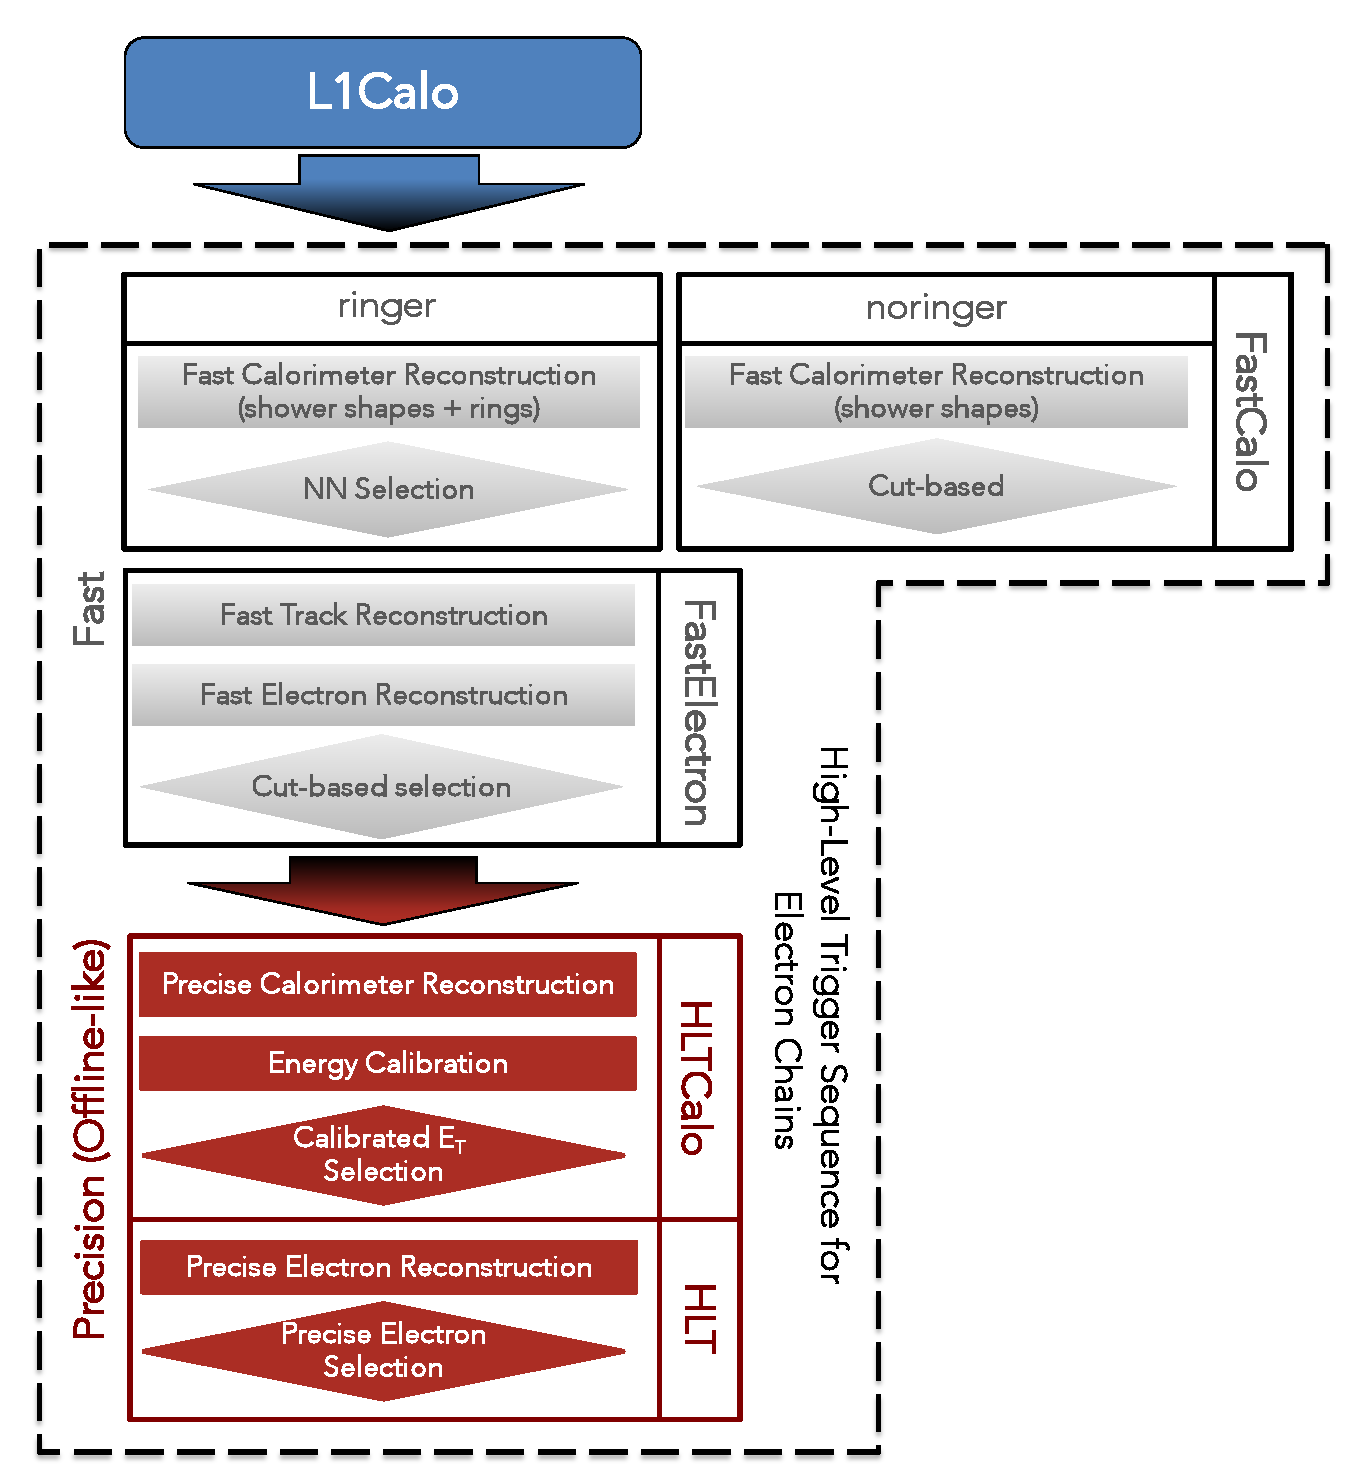
\includegraphics[width=0.7\textwidth]{sections/01_introduction/figures/ElectronChain_Run2_noringer_and_ringer.pdf}
  \caption{Comparison of the processing flow diagrams for the electron triggers with the logic employed in the triggers based on the cut-based strategy and the primary electron
  chains (ringer chains) since 2017, with the \rnn{} algorithm. The algorithms responsible for extracting some features from the event (also known as feature extraction) are represented by the red or gray rectangles. On the other hand, the algorithms responsible for making the decision to proceed to the next stage or not (called as hypothesis tests) are represented by the red or gray diamonds.}
  \label{fig:electron_chain}
\end{figure}




This paper describes the performance improvements due to introduction of the Neural-Ringer algorithm into the HLT fast calorimenter reconstruction step of the electron triggers, which became the baseline selection of events containing at least one isolated electron above 15 GeV in the 2017 proton-proton collision ATLAS data-taking. The Full details of its identification procedure are in Section~\ref{sec:neuralringer}, including the training and tuning strategies. The online performance results from the \rnn and the cut-based strategies are presented in Section~\ref{sec:operation} . A comparison of the \rnn with the cut-based triggers using statistical methods through the offline perspective is performed in Section~\ref{sec:off_ana}. Finally, the conclusions and prospects 
are derived in Section~\ref{sec:conclusion}.
 % ok
\section{The \rnn{} Algorithm}%
\label{sec:neuralringer}


\subsection{Building the Rings}\label{ssec:rnn_for_online_and_eletrons}


The ATLAS calorimeters comprise rectangular cells in the
\etaphi plane for different layers in depth\footnote{Except for the forward calorimeters.}.
The calorimeter system covers the pseudorapidity\footnote{ATLAS uses a right-handed coordinate system with its origin at the nominal interaction point (IP) in the centre of the detector and the z-axis along the beam-pipe. The x-axis points from the IP to the centre of the LHC ring, and the y-axis points upward. Cylindrical coordinates (r, $\phi$) are used in the transverse plane, \phi being the azimuthal angle around the beam-pipe. The pseudorapidity is defined in terms of the polar angle $\theta$ as \eta = -$\ln{tan(\theta/2)}$. The angular distance $\Delta R$ is defined as $\Delta R = \sqrt{(\Delta\eta)^{2} + (\Delta\phi)^{2}}$ . Transverse momenta and energies are defined as $pT = p\sin\theta$ and $E_{T}$ = $E\sin\theta$, respectively.} range \(|\eta| < 4.9\)~\cite{PERF-2007-01}. 


Within the region $|\eta|< 3.2$, an electromagnetic calorimetry (ECAL) is provided by the high-granularity lead/Liquid-Argon (LAr) calorimeters contituted of barrel (EMB1,2,3) and endcap (EMEC1,2,3), with an additional thin LAr presampler (\ps) covering in barrel (PreSamplerB) and endcap (PreSamplerE), in order to correct for energy losses in material upstream of the calorimeters~\cite{LARG-2009-01,larg_tdr}. The Hadronic calorimetry (HCAL) is provided by the steel/scintillating-tile calorimeter (\tilecal)~\cite{TCAL-2017-01,tile_tdr}, constituted of three barrel structures (TileBar0, TileBar1 and TileBar2) within $|\eta| < 1.0$, three extended barrel structures (TileExt1,2,3) covering the region of $0.8<|\eta|< 1.7$ and two copper/LAr hadronic endcap calorimeters (HEC)
~\cite{cal_tdr} within $1.5<|\eta|< 3.2$ divided in four modules (HEC0,1,2,3). Transition regions between calorimeters are used to locate detector services and induce a sharing of showers between calorimeters that degrades energy measurements in those regions. Here, the transition from the barrel to the endcap is complemented by the intermediate tile calorimeter (ITC) composed by two modules (TileGap1,2,3) that are both attached on the face of the external barrel to estimate signal losses~\cite{cal_tdr}. The solid angle coverage is completed with forward
copper/LAr and tungsten/LAr calorimeter (FCal) modules optimised for electromagnetic (EM) and hadronic (HAD) measurements, respectively. The specified calorimeters
provide full azimuthal ($\phi$) coverage with a total of about 190,000 readout cells. 



The electromagnetic and hadronic calorimeters are segmented~\cite{PERF-2007-01}\footnote{The two
central layers in HCAL end-cap are summed to result in a single measurement.} longitudinally (i.e. in depth) into three sampling layers each where each layer has its own lateral ($\eta\times\phi$) granularity. Besides granularity, the amount of detector material in front of the detector in each sampling layer also varies with \abseta, leading to variations in the expected lateral and longitudinal profiles. Additionally, the expected
profile is also dependent on the physics object total energy. In the EM calorimeter, most of the EM shower energy is collected in the second layer (EM2), while the third layer (EM3) provides measurements of energy deposited in the shower tails. Although, it is important to mention that the first EM layer (EM1) plays an important role in the discrimination of electrons against $\pi^0$. The hadronic calorimeters, which surround the EM detectors, provide additional discrimination power through further energy measurements of possible EM shower tails, as well as rejection of events with activity of hadronic origin with three sampling layers (HAD1,2,3). 


As the algorithm was considered to operate online at \fastcalo{} stage in software, approximations were made. Specifically, the rectangular rings are constructed to match the grid layout of the calorimeter cells and the ring coverage is bounded by the RoI area. In addition, granularity changes from the cell sizes from different regions of the detector are neglected\footnote{The $\eta$ granularity used by the algorithm at EM1 layer is 0.003 for the entire eta range defined ($|\eta|<2.5$). However, the detector construction at this layer cover the region of $0<|\eta|<2.37$ and has different granularities in $\eta$: starts with 0.003 at $0<|\eta|<1.81$; 0.004 at $1.81<|\eta|<2.01$ and 0.006 at $2.01<|\eta|<2.37$.} in order to employ a grid-like algorithm.


Here, the algorithm RoI covers a
region of the calorimeter, centered in the L1 provided RoI, of
$0.4\times0.4$ in the $\eta\times\phi$ plane. The algorithm
starts on the second EM sampling layer (EM2)\footnote{This convention is used for all sampling layers, thus HAD1 stands for the first hadronic layer, HAD2 the second hadronic layer etc.}, where position given in $\eta\times\phi$ plane of the cell with highest $E_T$ on the algorithm RoI is taken as the center of the cascade interaction in the calorimeter. The initial seed cell position is propagated to other calorimeter layers in order to define the axis of the rings in that layer. Then, for each layer, the algorithm refines the seed position searching for most energetic cell inside of the window centred on the EM2 initial seed and the energy deposition of an incoming particle is extracted by building concentric rings of cells, or simply ``rings''. 

\begin{figure}[h!t]
	\centering
	\begin{center}
		\begin{subfigure}[c]{.95\textwidth}
			\centering
			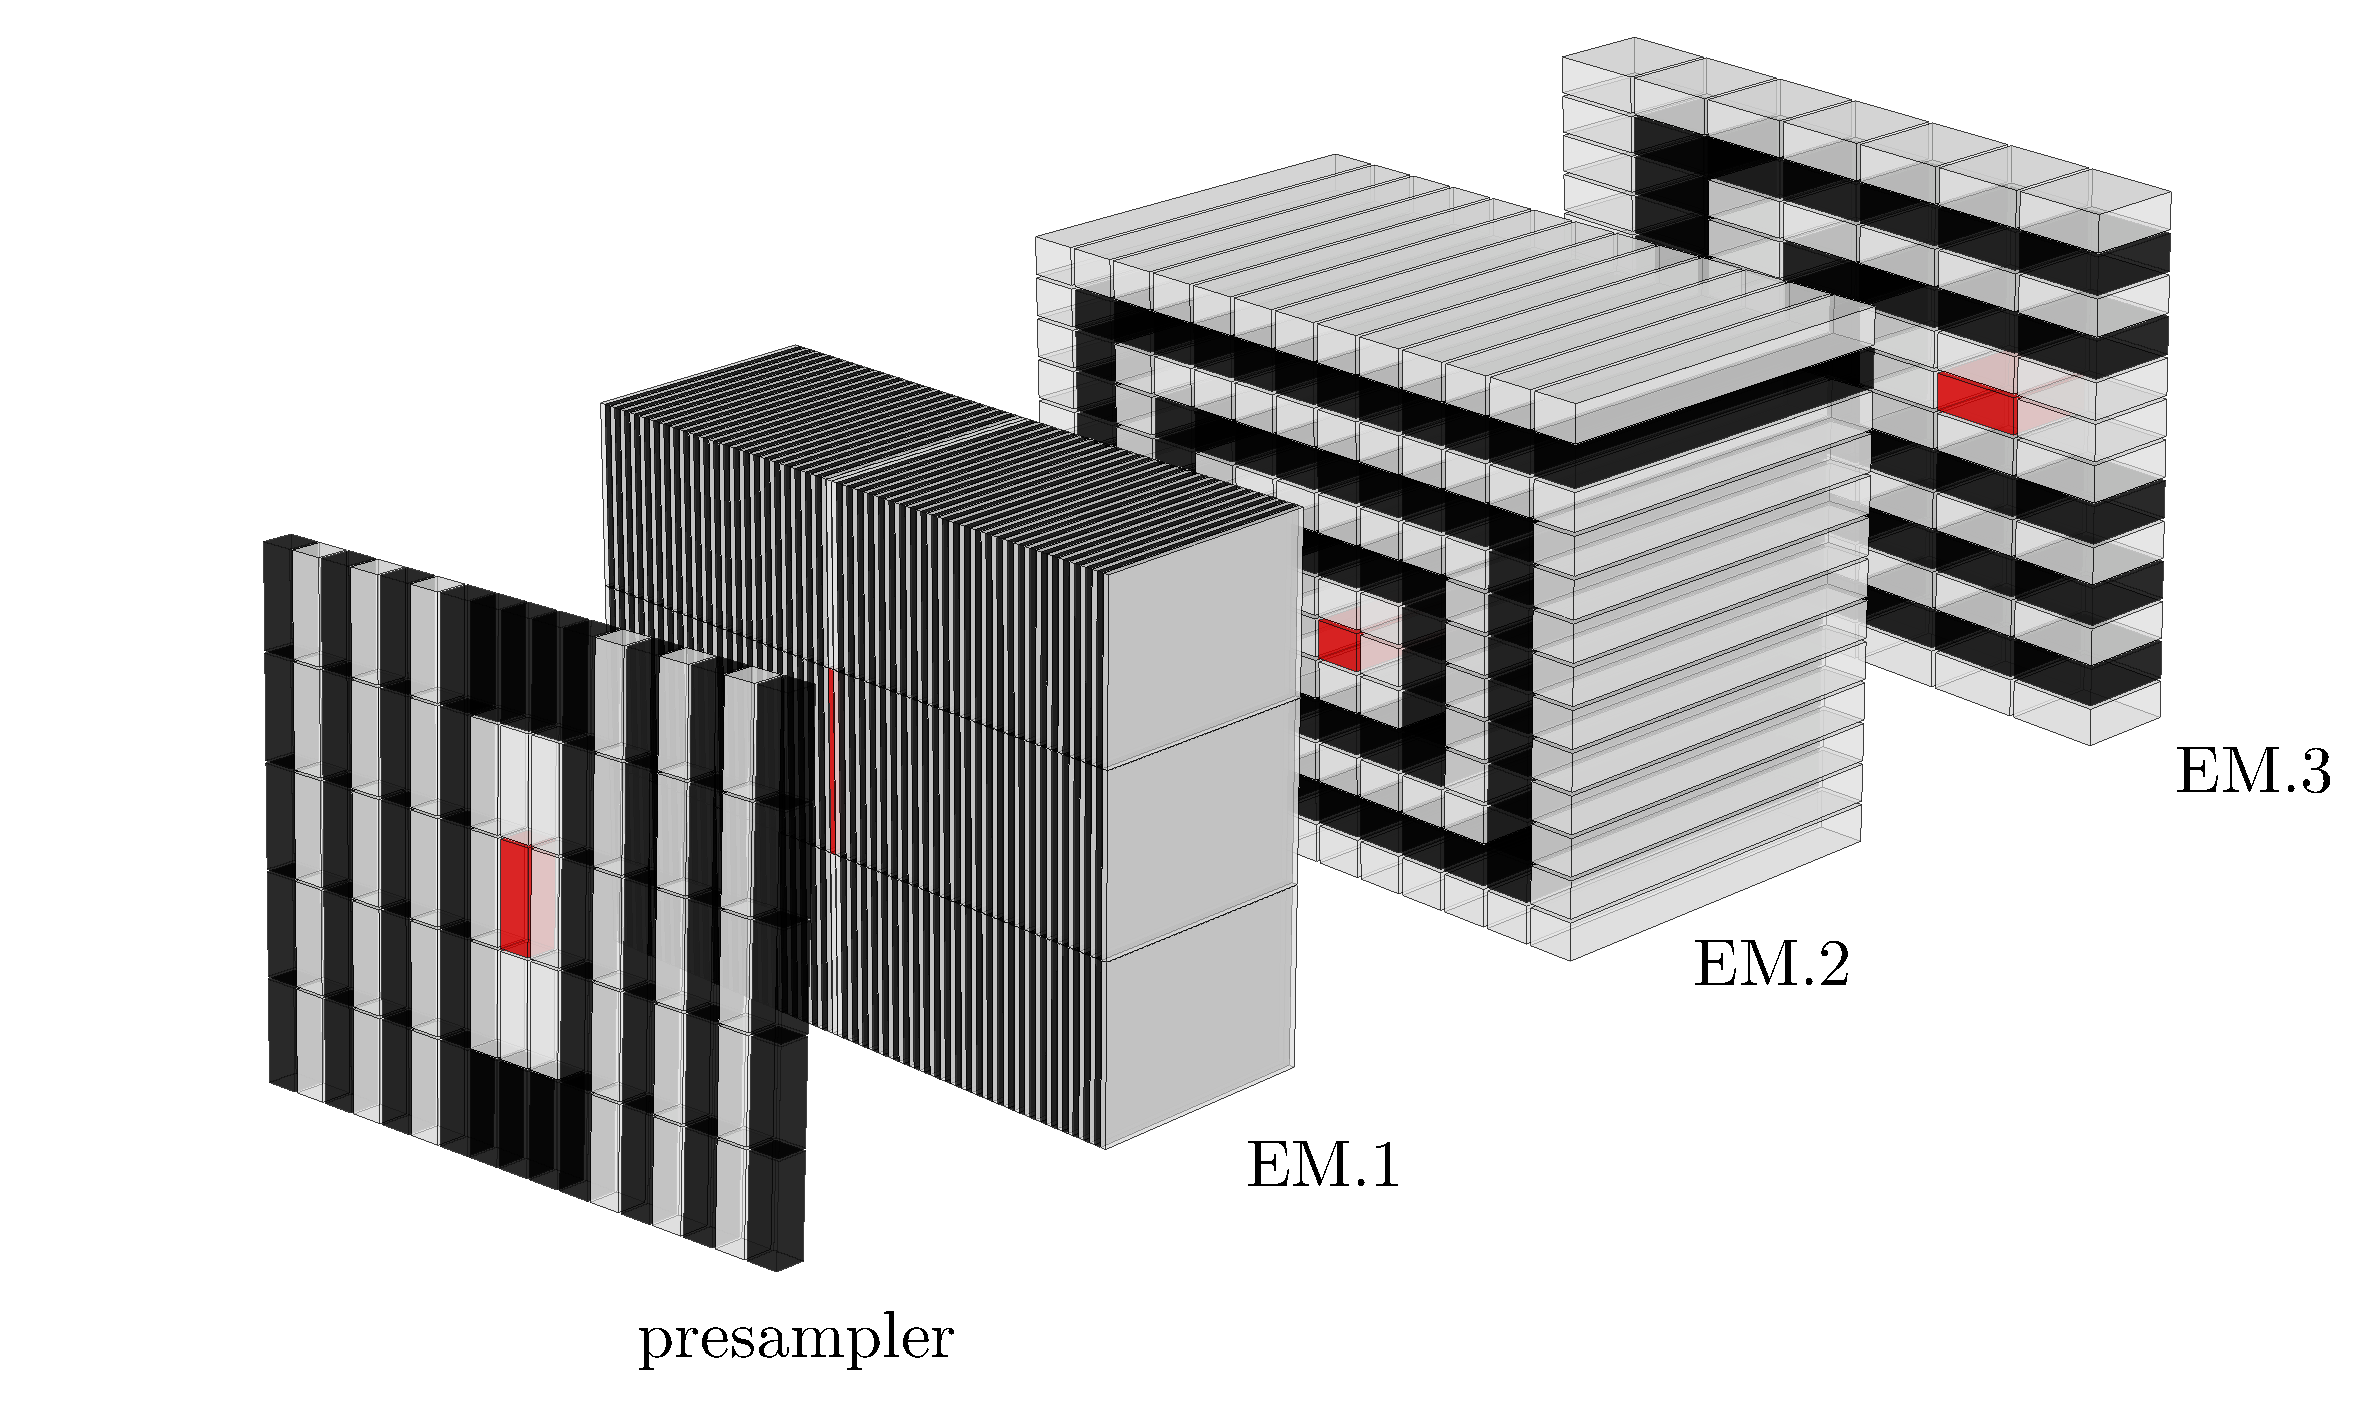
\includegraphics[width=\textwidth]{sections/02_ringer/figures/ATLAS_EM_Layers_v5.pdf}
			\caption{Eletromagnetic calorimeter cells within the ringer reconstruction window.}
		\end{subfigure} \\
		\begin{subfigure}[c]{.95\textwidth}
			\centering
			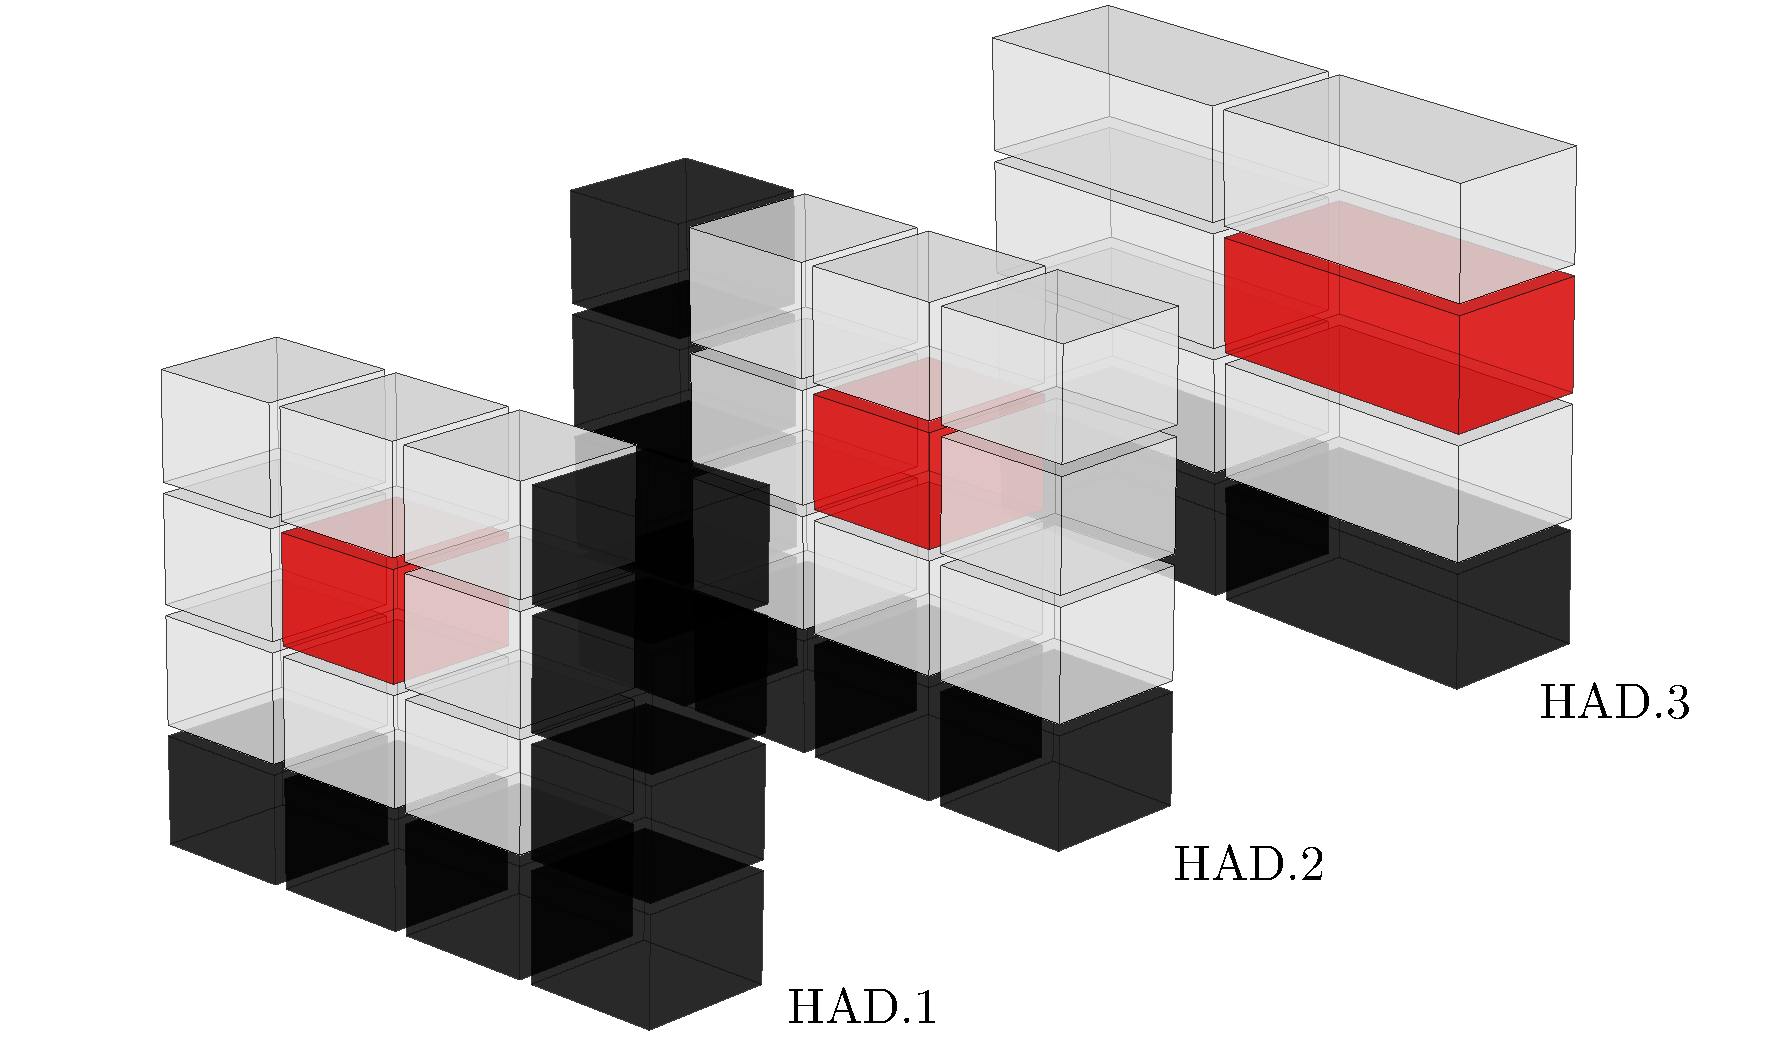
\includegraphics[width=\textwidth]{sections/02_ringer/figures/ATLAS_HAD_Layers_v5.pdf}
			\caption{Hadronic calorimeter cells within the ringer reconstruction window.}
		\end{subfigure}
	\end{center}
	\caption{\label{fig:calo_rings}
		Sketch to illustrate the ring-shaped energy description.
		The most energetic cell is in red, while the consecutive neighbouring rings are represented by alternating gray and black cells.
	}
\end{figure}

The refined seed ($c_{hot,l}$) will be used as starting point to build the rings. A ring $R_{n,l}$ contains all cells in calorimeter layer $l$ which are $n$ cells from the refined seed (See \figurename~\ref{fig:calo_rings} for an illustration of the parameters). Formally,


\begin{equation}
%\label{eq:ring_idx}
R_{n,l} = \left\{c_{n,l} \mid n = \left\lfloor \max{\left( 
\frac{| \eta_{i,l} - \eta_{hot,l} |}{h_{\eta,l}}, 
\frac{| \phi_{i,l} - \phi_{hot,l} |}{h_{\phi,l}} 
\right)} \right\rceil, 
\forall c_{i,l} \in
\Theta_{RoI,l}
\right\},
\end{equation}



\noindent where (analogous to $\phi$ when suitable): $\eta_{i,l}$
and $\eta_{hot,l}$ are respectively the $c_{i,l}$ and $c_{hot,l}$
cells position in $\eta$; $h_{\eta,l}$ is the $l^{th}$ layer cell size in $\eta$; $\Theta_{RoI,l}$ is the set of cells
in the $l^{th}$ layer which are within the Ringer RoI and $\lfloor \cdot \rceil$ is the \textit{round} function.
\tablename~\ref{tab:ring_alg_parameters} shows the number of rings computed at each layer and the respective granularity.


\begin{table}[ht!]
\centering
\caption{Nomenclature defining the \rnn{} algorithm layers and sections, as well as the respective parameters employed and calorimeter sampling layers from which the cells are extracted. The \rnn{} algorithm parameters are dependent on the ringer layer $l$ and independent on \eta{} and \et{} during Run~2. The parameters are the ring size in \eta{} ($h_{\eta,l}$), $\phi$ ($h_{\phi,l}$) and the number of rings to be computed in each layer ($\text{N}_l$).
}%
\label{tab:ring_alg_parameters}
\resizebox{.8\textwidth}{!}{%
\begin{tabular}{lc|ccc|ccc}
\hline
\hline
\multicolumn{2}{c|}{Ringer} & \multicolumn{3}{c|}{Calorimeter Sampling} & 
\multicolumn{3}{c}{Parameters} \\
\hline
Section & Layer ($l$) & Barrel & \itc & End-cap & $h_{\etaa,l}$ & $h_{\phii,l}$ & $N_l$ \\
\hline
\hline
\multirow{4}*{EM} & \ps &  \presamplerb & & \presamplere & 0.025 & 0.1 & 8 \\
\cline{2-5}
& \emi & \emb{1} &  & \emec{1} & 0.003 & 0.1 & 64  \\
\cline{3-5}
& \emii & \emb{2} &  & \emec{2} & 0.025 & 0.025 & 8 \\
\cline{3-5}
& \emiii & \emb{3} &  & \emec{3} & 0.050 & 0.025 & 8 \\
\cline{1-5}
\multirow{6}*{HAD} & \multirow{2}*{\hadi} & \tilebar{0} &
\multirow{2}*{\tilegap{3}} & \multirow{2}*{\hec{0}} & \multirow{2}*{0.1} & \multirow{2}*{0.1} & \multirow{2}*{4} \\
&                     & \tileext{0} &                               &                           \\
\cline{3-5}
& \multirow{2}*{\hadii} & \tilebar{1} & \multirow{2}*{\tilegap{1}} & \hec{1}       & \multirow{2}*{0.1} & \multirow{2}*{0.1} & \multirow{2}*{4} \\
&                   & \tileext{1} &              & \hec{2}  \\
\cline{3-5}
& \multirow{2}*{\hadiii} & \tilebar{2} & \multirow{2}*{\tilegap{2}} & \multirow{2}*{\hec{3}} & \multirow{2}*{0.2} & \multirow{2}*{0.1} & \multirow{2}*{4} \\
&                     & \tileext{2} &                &             \\
\hline
\hline
\end{tabular}
}
\end{table}

The sum of the transverse energies of cells $c_{n,l}$ in the ring $R_{n,l}$ form a vector of discriminating quantities. They are ordered outwards and from the innermost layer of the calorimeter and provide the ring-shaped information of the RoI.




The ring building process resulting in 100 rings in total across all calorimeter layers. Thereby, a dimensionality reduction is provided by compacting the typical input space dimensionality of approximately 1000--1200 cells per ROI into the above-mentioned 100 rings through the usage of EM shower physics knowledge: the rings can keep a complete description of the symmetric lateral and longitudinal information. However, the algorithm only approximates this concept in order to meet the online operation requirements and avoid further manipulation of the instrumented information. 
Figure~\ref{fig:rings_profile} shows the ring-shaped mean profile differences between electrons and jet particles. 



\begin{figure}[!ht]
  \centering
  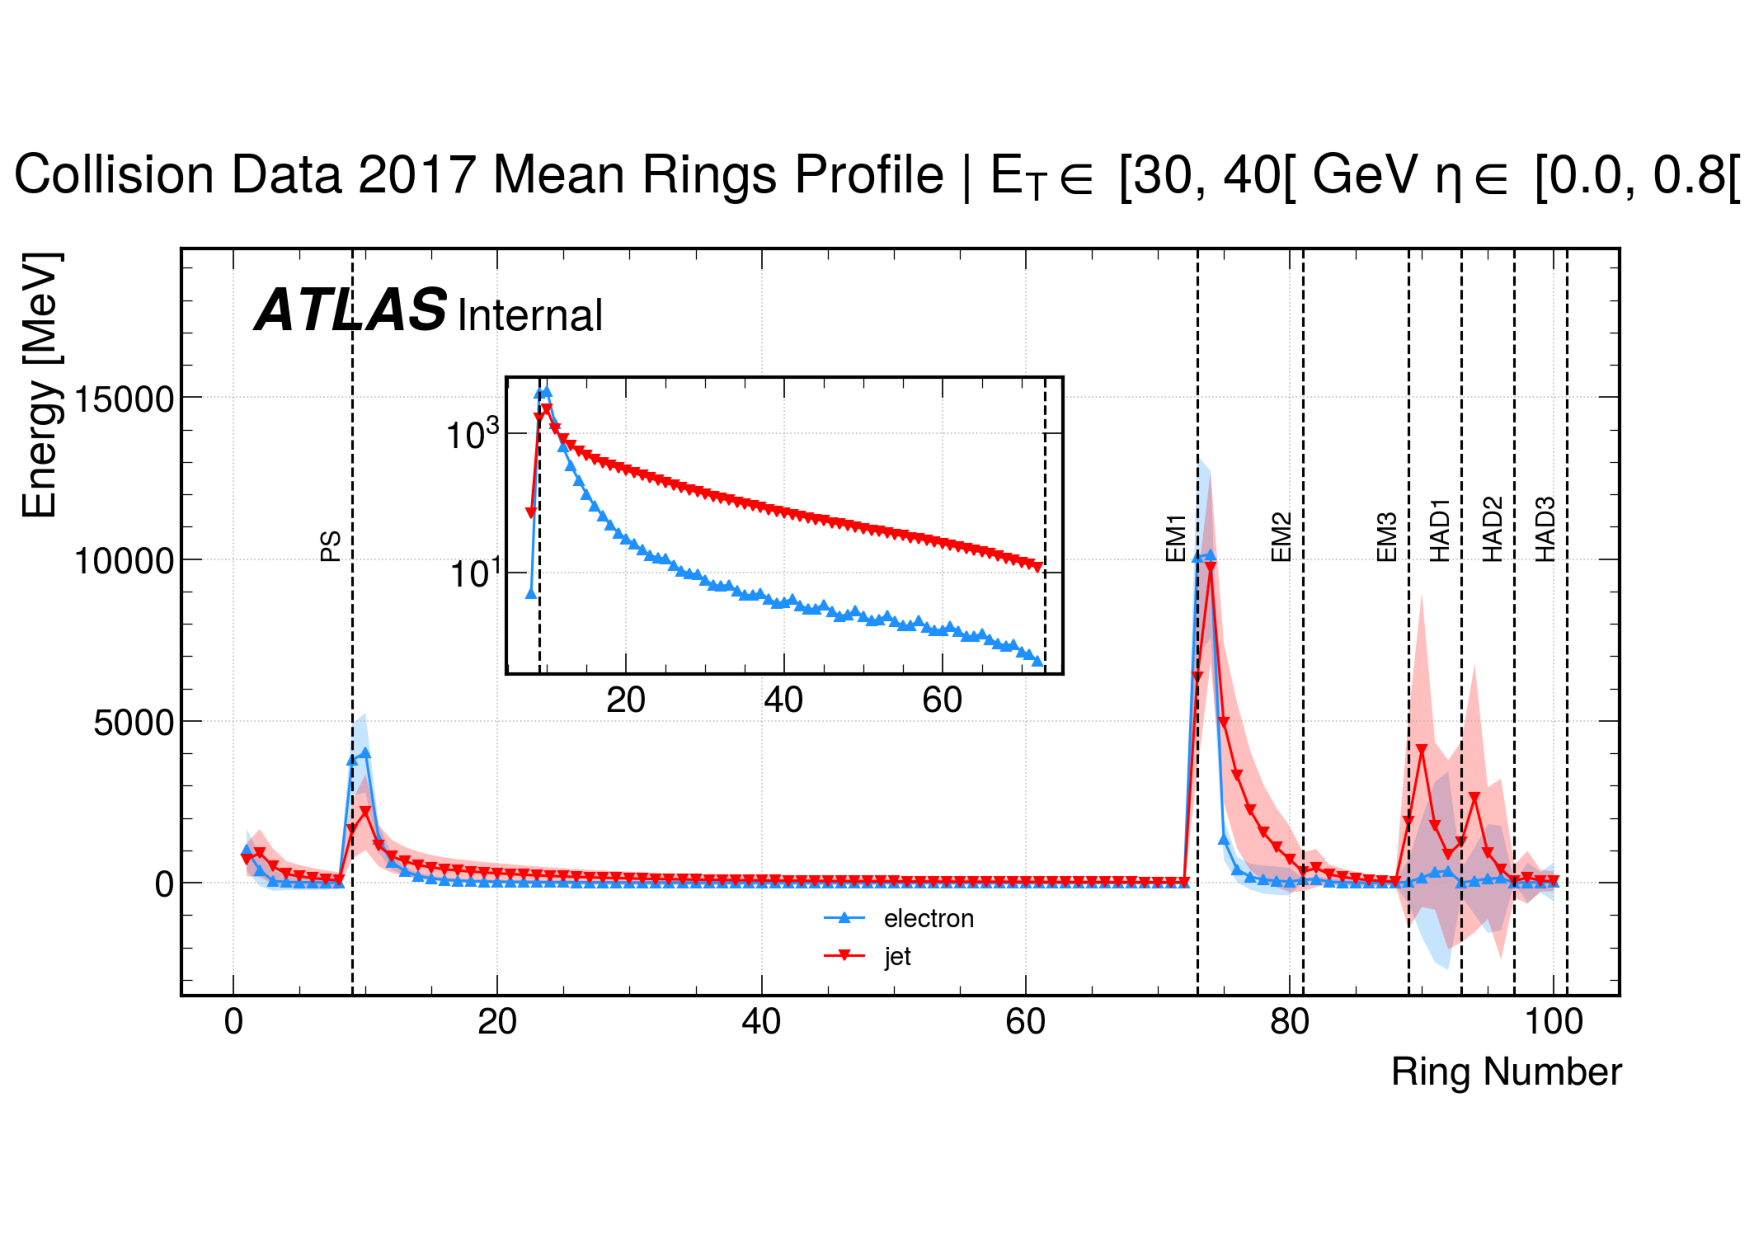
\includegraphics[width=0.7\textwidth]{sections/02_ringer/figures/reco_steps/data17_zee_mean_rings_profiles_et2_eta0.pdf}
  \caption{Average ring profile from collision data at $30 \leq E_T < 40$ GeV and $0.0 \leq \eta < 0.8$ for each layer of the calorimeter. The embedded profile shows the EM1 layer ring energies in a logarithmic scale. Here, it is possible to observe that most part of the energy for the electrons is absorbed by the eletromagnetic layers. For the jets, the opposite is observed and most of the energy is absorbed by the hadronic layers.}
  \label{fig:rings_profile}
\end{figure}

\subsubsection{Ring Sums as Discriminant Variables}

The current strategy concatenates all rings in a single vector of 100
variables. An absolute normalization using the total RoI energy is applied to normalize the variables. 
This procedure was initially proposed and examined by~\cite{1995_seixas_ringer}, as a way of preserving the shower energy profile in fractions of the total energy. 
The absolute value is used to avoid reflecting the values along the axis due to negative noise accumulation, a behavior which would impact the physics
representation of the normalized values and require a more complex decision
boundary:

\begin{equation}
  r^\prime_{k} = \frac{r_{k}}{| \sum\limits_{i=1}^{100} r_i
  |}, \;\;\;
    \forall \; k\in\{1,\dots,100\}.
\label{eq:ring_norm}
\end{equation}

Where $r_k$ or $r_i$ is the transverse energy of the ring with index $k$ or $i$ and $r^\prime_{k}$ is the normalized ring value with index $k$. It is specially valuable for its simplicity as it uses of a non parametric approach, and for allowing easy interpretation of the shower profile.



\subsection{Motivation for a Set of Neural Networks}\label{ssec:nn_set}

The normalized concatenated ring vector feeds a set of MLPs. A single
model is drawn from the set for operation based on the nearest region on the \eteta space for which it was designed.

In regards to calorimetry, the usage of a set with specific models per phase space region allows to mitigate fluctuations in the variable profiles
due to the detector response and energy differences of the showers.
A large contribution comes from granularity changes, which are discrete
in the phase space. Other important factors 
influencing such profiles are the
amount of the material as a function of \abseta{} and the dependence of
underlying processes in the shower development with respect to the incoming
particle energy. Although these alterations are mostly continuous, it is also
possible to approach the problem using space discretization.



At the hardware resource level, splitting the training into multiple small models to accommodate inhomogeneity of the detector response speeds up the training cycle and allows to handle data in memory, since only a small portion of the data is used to train that specific model. Limiting the memory requirement for tuning the models is particularly interesting in order to benefit from low-memory processing nodes, which were predominantly available in 
WLCG~\cite{2015_lcg_tdr} during our developments.\@ In addition, the decomposition of the problem can also lead to a reduction of the training time~\cite{Polikar2006}, as observed heuristically\footnote{
  When using NVIDIA RTX 2080Ti in tensorflow 1.14 and a minibatch size of 1024, a MLP with single hidden layer, a substantial increase in the runtime (from 4 to 41 seconds per epoch) with respect to the set version was observed.} 
when comparing the tuning time of the set to a single model. 
Regarding the operation, the proposed set only requires the choice of a
single model to operate instead of a more often committee machine approaches
that require the computation of different models in parallel with a fusion
method~\cite{zhou_ensemble}.  Therefore, the chosen set configuration adds
minimal overhead in terms of trigger latency. Similarly, the choice was to
operate with low-complexity models, a single hidden layer with few neurons, to obtain a competitive method with respect to the cut-based approach, in terms of processing speed.



\subsection{Training and Decision Making for 2017 and 2018 Operation}%
\label{sec:tuning}

\subsubsection{Data sets and Event Selection}%
\label{ssec:dataset}

The training procedure for 2017 operation was built with samples of 2015 simulated $Z\rightarrow ee$ decay, selected by the $Z\rightarrow ee$ \TnP method\cite{aad2020performance}, and background. For simulated background samples, a filter was applied to enrich with particles produced in the hard scatter with a summed transverse energy exceeding 17 GeV in a region of $\Delta\eta\times\Delta\phi=0.1\times0.1$. During 2016 data taking, the pile-up reached was 40 interactions per bunch crossing.
Here, both simulated samples include a pile-up of 60 interactions in average, per bunch crossing, which had never been seen before in collision data until the end of 2017, when the observed peek pile-up exceeded 60. Recently, in 2023, the highest level of pile-up observed exceeded 60 again.

After the training stage, thresholds on the discriminating score must be determined for selection of good electron candidates. To set the correct value without causing any inefficiency in the end of the HLT in collision data, the probe electrons, selected by $Z\rightarrow ee$ \TnP method and approved by the tightest offline available criteria, from full \textit{pp} data recorded by ATLAS in 2016 with LHC operating at a centre-of-mass energy of $\sqrt{s}=13\text{ TeV}$ was used. For background, objects rejected by the $Z\rightarrow ee$ \TnP method, that does not belong to any tag-probe electron pair, and reproved by the loosest offline available criteria were used. For the 2018 operation, the purely data-driven strategy was used, selecting events from the 2017 recorded collision data to train the models and adjust all thresholds. The tuning and analysis performed on collision data recorded have their quality ensured by the data quality procedure. 


\subsubsection{Training and Decision Making}%

The 2017 procedure derived the MLP models with simulated samples and defined the discriminant cut using 2016 collision data, targeting a signal efficiency similar to that of the cut-based trigger. The training procedure and decision making processes are the same for all phase space regions. For the \rnn{}, each MLP is an expert model for a single phase space region, containing its own topology and parameters.

The model parameters have been optimized using events selected on simulation datasets (Section~\ref{ssec:dataset}). 
The structure is a fully-connected single hidden layer, which may contain from 5 to 20 hidden units, an input layer with 100 inputs, one for each ring, and an output layer with a single neuron. 
The activation functions for both hidden and output neurons are the hyperbolic tangent, which has been often used in MLP designs~\cite{haykin_2008}. 

To assess the statistical fluctuations of the efficiency measurements, the stratified k-fold ($k=10$) cross-validation method~\cite{haykin_2008} was used at the price of increased computational cost by repeating training and testing procedures on different randomly chosen subsets. 
The stratified k-fold is among the most common cross-validation techniques and consists of partitioning the dataset in k disjoint subsets, each model tested with the $i$th subset and trained with the remaining ones. The dataset stratification follows the empirical order of the event selection, in order to allow straightforward job parallelization, i.e.\ random permutation is not employed. 

For each cross-validation sort and working point, 100 networks, initiated as from~\cite{initnw}, are optimized by back-propagating the Mean Squared Error (MSE) through the RPROP algorithm~\cite{rprop}. This repeated model initialization aims at avoiding poor sub-optimal solutions due to the usage of gradient-based algorithms.
For each training procedure, only three models out of the 100 are retained: two for retrieving the best efficiency when fixing the sensitivity or false positive probabilities to the baseline \fastcalo{} efficiency and another resulting in the \spmax{}\footnote{The SP value is defined as $\sqrt{\sqrt{P_D(1-F_A)}\cdot\frac{P_D + (1-F_A)}{2}}$ where $P_D$ is the signal detection probability (or sensitivity) and $F_A$ is the probability of a fake signal (false positive).} value. Early stopping~\cite{haykin_2008} is employed to avoid model over-training. The selection of the optimal iteration and operating model is based on an heuristic approach (multi-stop)~\cite{Goodfellow2016}.


Computational resources were used to tune 1.3~M shallow-learning neural networks, which resulted in a set of \SI{20}{MLPs} (five in \et{} $\times$ four in \abseta{}) for each one of the four working points used by electron triggers in the HLT. 
Here, the first training strategy considered only four regions in $|\eta|$ ($0.0\rightarrow 0.8\rightarrow1.37\rightarrow2.5$) and five region in $E_T$ ($15\rightarrow 20\rightarrow 30\rightarrow 40\rightarrow 50\rightarrow\infty$).
Except for few exceptions, the models in the set employed 5 neurons in the hidden layer. 

After the training stage, the decision is taken by applying a threshold in the one-dimensional output node of each expert MLP. 
Inspired by the HLT likelihood algorithm, the threshold applied for \rnn is also computed as a linear function of \avgmu{}.
However, a non-linear behavior was observed near the asymptote of the output activation function (See Figure~\ref{fig:nn_correction_with_tansig}), which occurred for the medium and tight operation points. Heuristically, it was 
observed that this behaviour can be avoided when replacing the hyperbolic tangent activation function from the output neuron by a linear function (Figure~\ref{fig:nn_correction_without_tansig}) for operation, after the training stage is completed.
This strategy provides a linear behavior of the targeted signal efficiency with respect to the online pile-up estimator. 
To account for Monte Carlo and collision data mis-modeling (See Figure~\ref{fig:nn_mc15_vs_data16}), the parameters of the linear threshold correction were derived using 2016 collision data and upper-bounded\footnote{in case of pile-up higher than upper-bound, the corrected threshold value is fixed.} by $\avgmu=40$ collisions. 


\begin{figure}[h!tb]
  \begin{center}
  %\hspace{0.01\textwidth}
  \begin{subfigure}[c]{.48\textwidth}
  \centering
  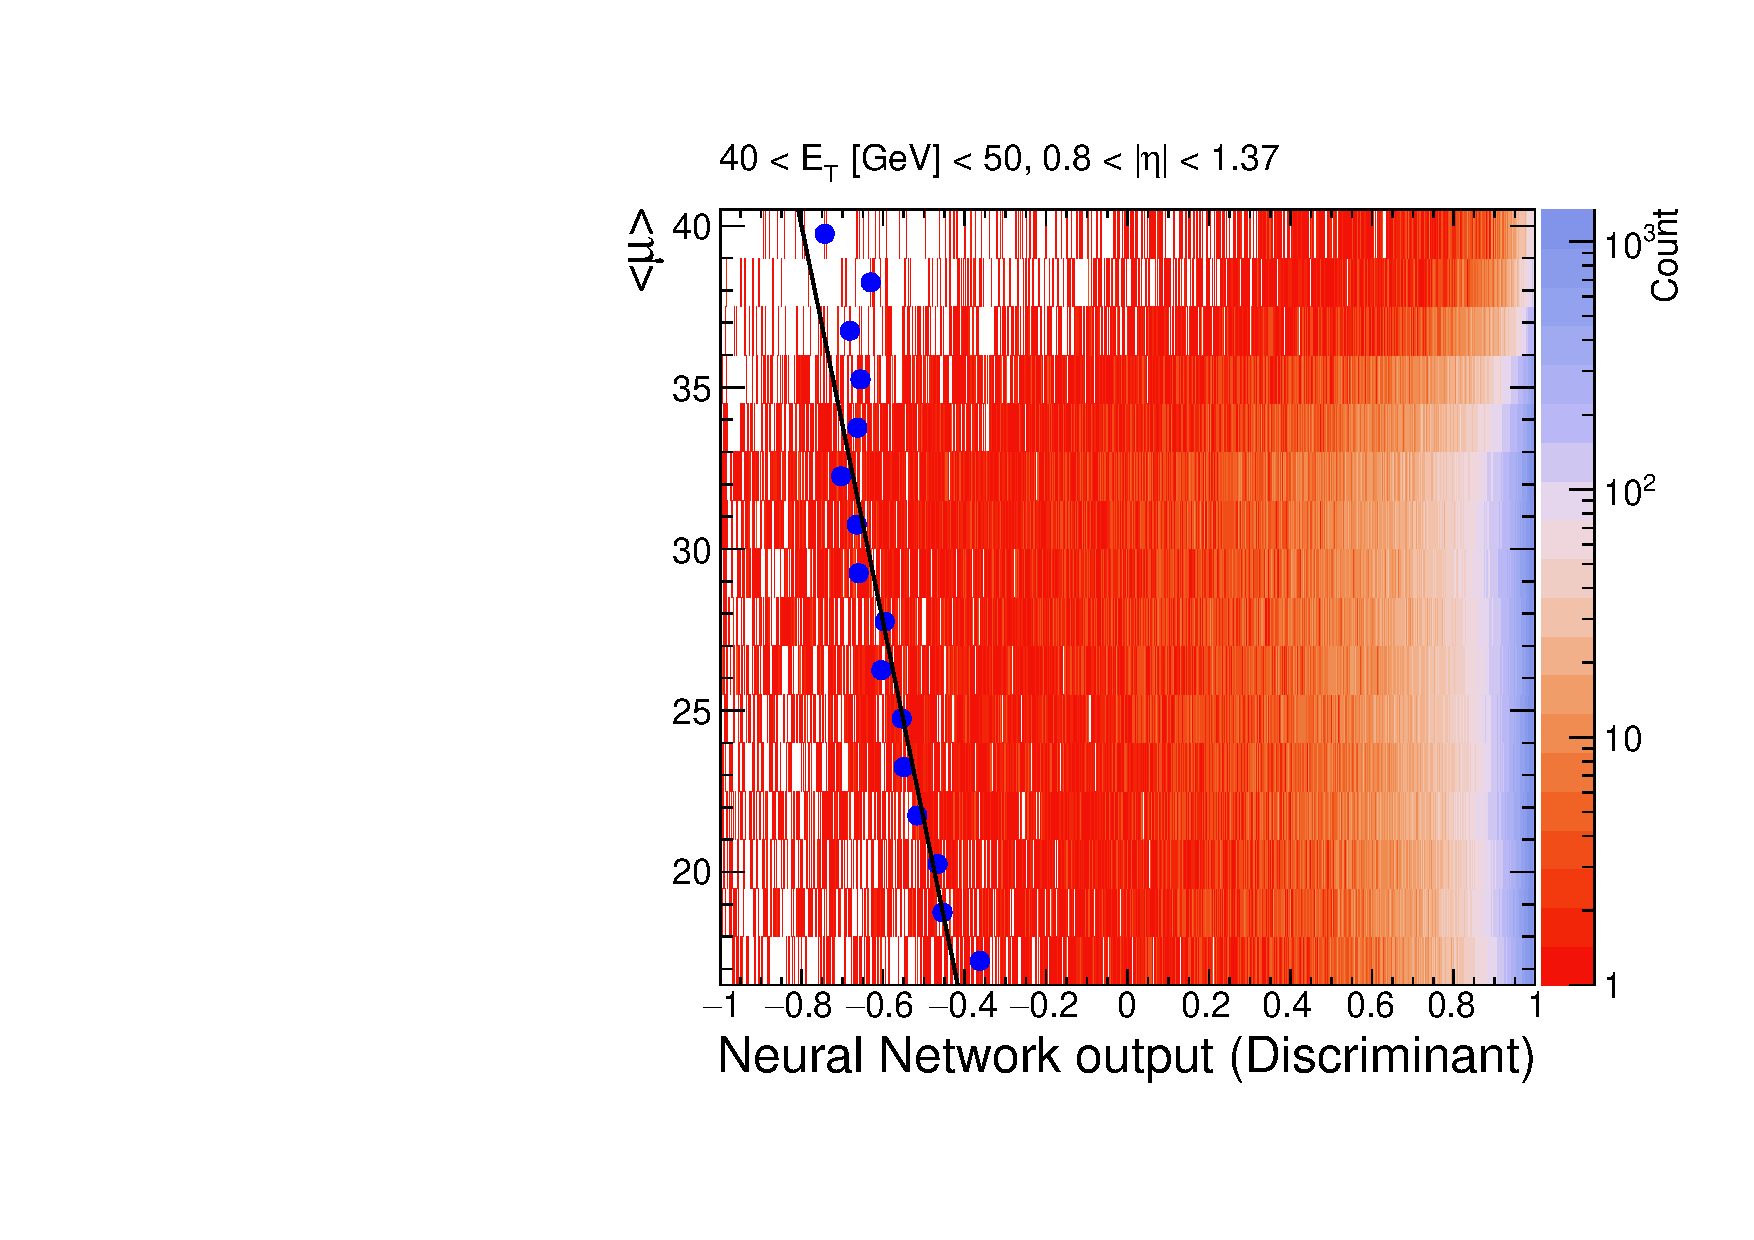
\includegraphics[width=\textwidth]{sections/02_ringer/figures/th2_signal_tight_cutbased_et3_eta1_with_tansig.pdf}
  \caption{MLP output with hyperbolic tangent as activation function in the output neuron w.r.t pile-up.}
  \label{fig:nn_correction_with_tansig}
  \end{subfigure}
  \hfill
  \begin{subfigure}[c]{.48\textwidth}
  \centering
  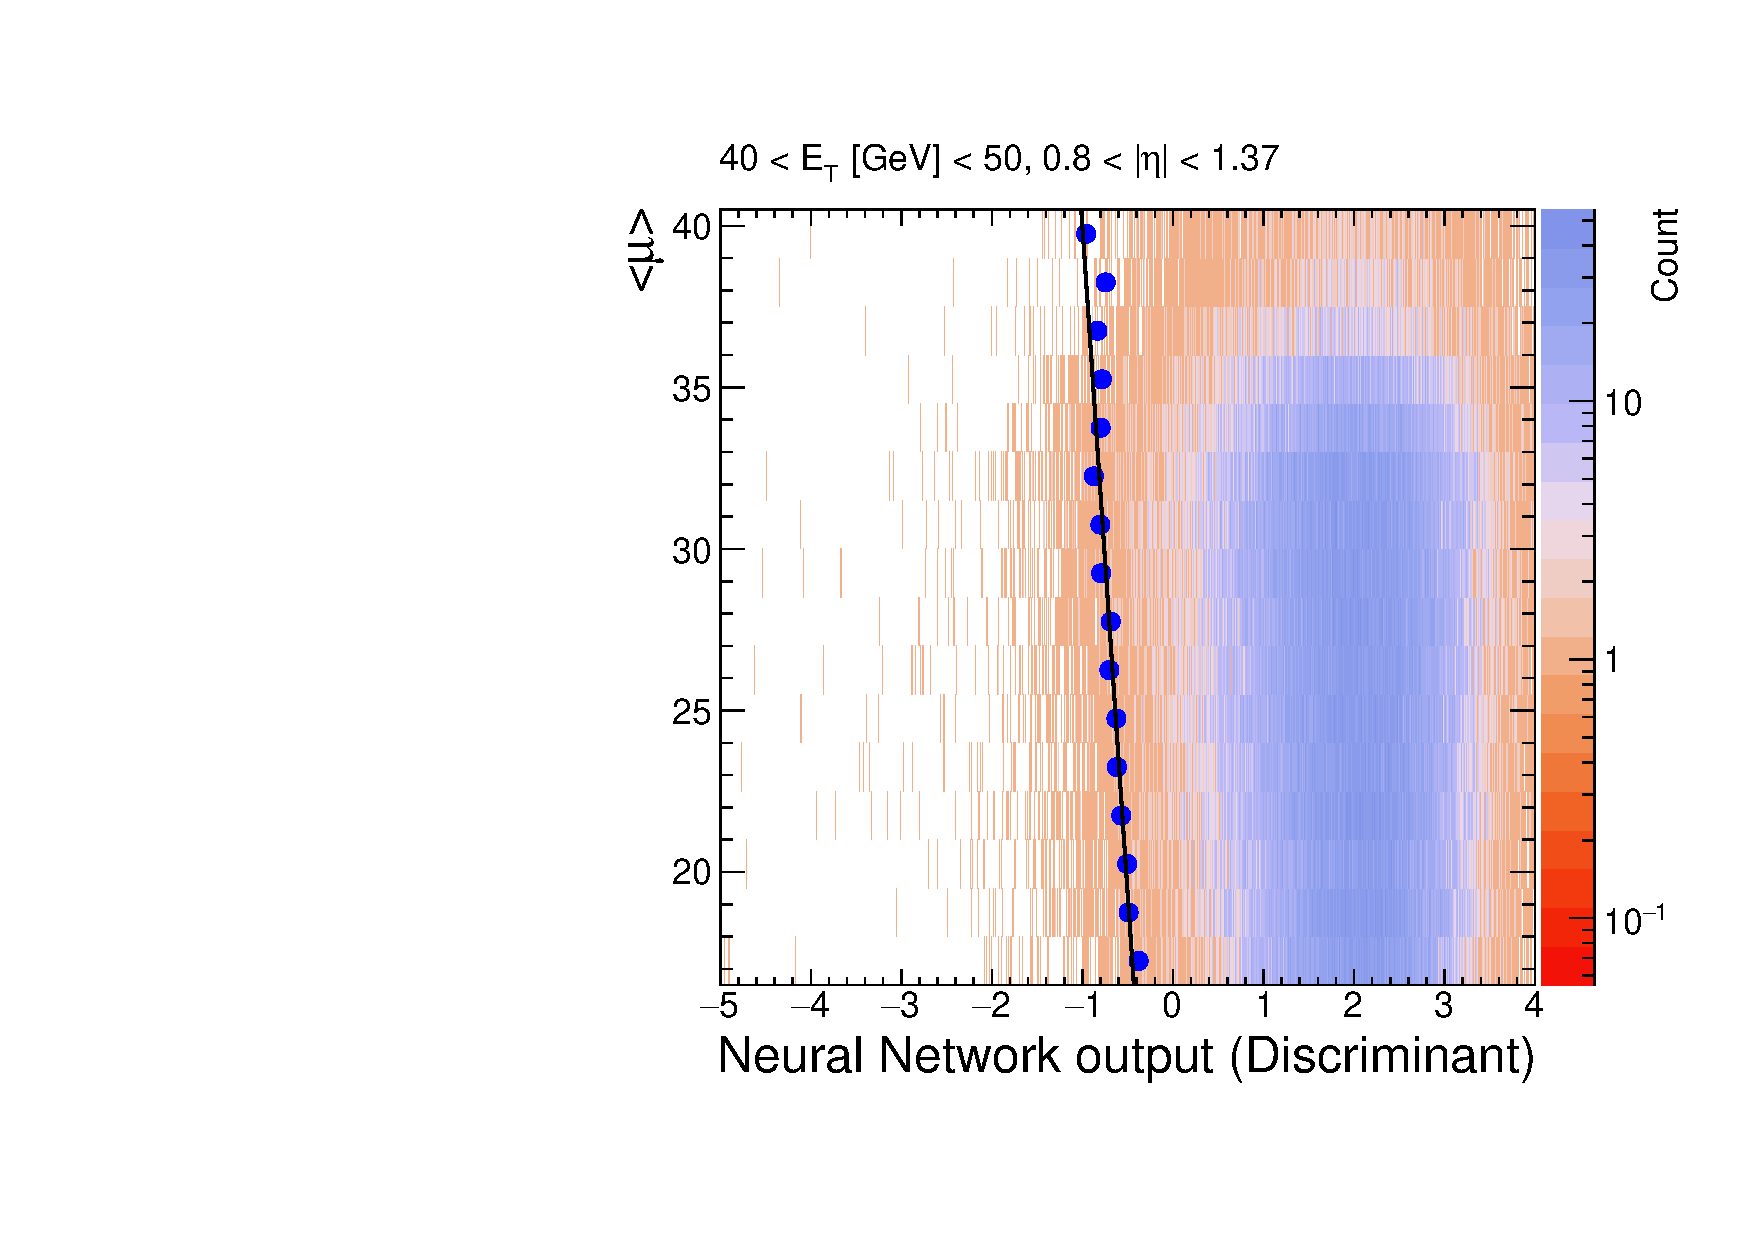
\includegraphics[width=\textwidth]{sections/02_ringer/figures/th2_signal_tight_cutbased_et3_eta1_without_tansig.pdf}
  \caption{MLP output with linear activation as activation function in the output neuron w.r.t pile-up.}
  \label{fig:nn_correction_without_tansig}
  \end{subfigure}
  %\hfill
  \caption{
    \rnn output as a function of \avgmu{} for $Z\rightarrow ee$ probes in 
    2016 collision data selected using the training criteria.
    The computed threshold per \avgmu{} unit for achieving the target 
    efficiency is shown in blue full circle. The black line is a linear fit of the thresholds.
    The output space is computed using the trained model without modifications 
    in (a), while in (b) the activation function from the output neuron is replaced by a linear function.
  }%
  \end{center}
\end{figure}

\begin{figure}[!ht]
  \centering
  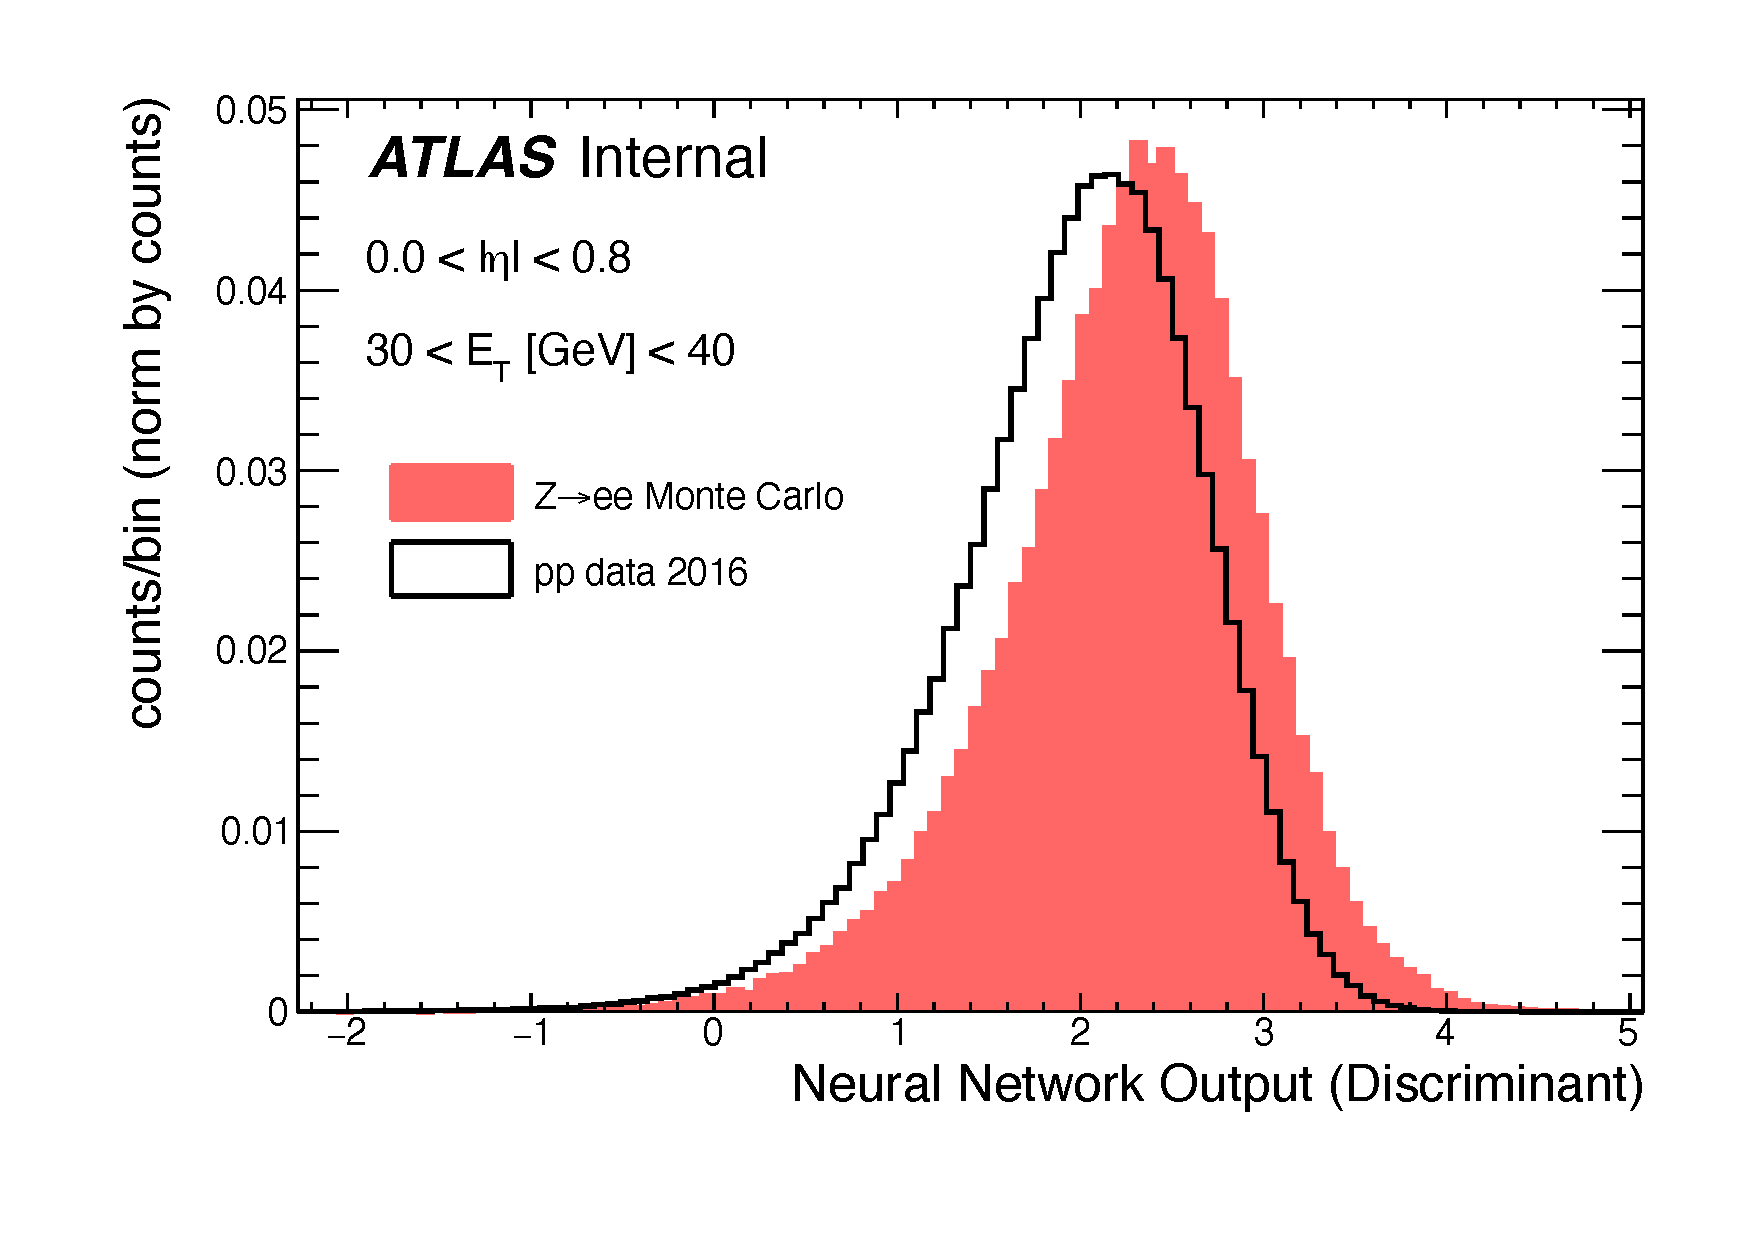
\includegraphics[width=0.7\textwidth]{sections/02_ringer/figures/nn_output_mc15_versus_data16_et2_eta0.pdf}
  \caption{Differences between simulation samples (red) from 2015 and collision data (black) obtained in 2016 for a region of the phase space.
  The comparison is made between the normalized distributions obtained in both cases for the output of the neural network (discriminant) generated for the samples present in the signal set within the selected region of the phase space. The shift on the discriminant generated by the neural network between simulation and collision data is caused by the differences of the simulation-data rings used as input of the model. }
  \label{fig:nn_mc15_vs_data16}
\end{figure}


Furthermore, it was observed
that the rings in the region $2.37<\abseta<2.47$ had particular profiles due to
the lack of strip cells in this region and demanded a specific discriminant requirement in order to keep signal efficiencies close to the cut-based triggers. In order to avoid retraining all models, it was decided to split the last $|\eta|$ region in two, from $1.37\rightarrow 2.5$ to $1.37\rightarrow2.37\rightarrow2.5$, and duplicate all models, for this region, to the new bin. Finally, the set used to operates in 2017 has a total of 25 MLP models. The set boundaries are defined by Table~\ref{tab:ensemble_regions}.



\begin{table}[htb]
\begin{center}
	{\small
	\begin{tabular}{cccc}
		\hline \hline
		\multicolumn{4}{c}{Model Adjust}                                                                 \\ \hline
		\multicolumn{2}{c|}{$E_T$ {[}GeV{]} Boundaries} & \multicolumn{2}{l}{$|\eta|$ Boundaries}        \\ \hline
		\multicolumn{2}{c|}{$15 \leq E_T < 20 $}        & \multicolumn{2}{l}{$0.00 \leq |\eta| < 0.80 $}   \\
		\multicolumn{2}{c|}{$20 \leq E_T < 30 $}        & \multicolumn{2}{l}{$0.80 \leq |\eta| < 1.37 $}  \\
		\multicolumn{2}{c|}{$30 \leq E_T < 40 $}        & \multicolumn{2}{l}{$1.37 \leq |\eta| < 1.54 $} \\
		\multicolumn{2}{c|}{$40 \leq E_T < 50 $}        & \multicolumn{2}{l}{$1.54 \leq |\eta| < 2.37 $} \\
		\multicolumn{2}{c|}{$50 \leq E_T < \infty $}    & \multicolumn{2}{l}{$2.37 \leq |\eta| < 2.47 $} \\ \hline \hline
	\end{tabular}
}
\end{center}
\caption{$E_T$ and $\eta$ boundaries used to create the set of neural networks.}
\label{tab:ensemble_regions}
\end{table}

On the other hand, the 2018 training procedure employed a single set structure for all working points and used the 2017 collision data, selected with  \Zee{} \tnp{} event selection, for training, as was the case for the derivation of offline and final \hlt likelihood models~\cite{aaboud2019electron}.
Most of the procedure was kept unchanged for 2018. In opposition to 2017, the developments for 2018 could benefit from collision data representing similar data taking conditions. To simplify the training strategy, the selection of three models for each training was abandoned, keeping only the \spmax{} model, as the previous approach was more complex without a clear return on trigger efficiency. 

Likewise, MLPs with 5 to 10 units in the hidden layer were tuned, as most models did not require more than 10 units in 2017. The training optimizer was changed to the \emph{Adam}~\cite{kingma2014adam}, instead RPROP, and the MLP model topology was modified to: a hidden layer with a fully connected neurons with a rectified linear units (RELU) as the activation function and an output layer with one neuron using the sigmoid as the activation function. With a larger time span for entering operation, specialized MLPs in the region where a change was detected in the ring profiles before 2017 operation between $2.37<\abseta<2.47$ was added, resulting in the operation of \SI{25}{MLPs}. Finally, the correction limit was set to $\avgmu{}=100$~collisions in other to extrapolate the operation of the models to a never reached pile-up level condition. 





 % 
\section{Online Deployment and Performance}%
\label{sec:operation}


 During to 2017-2018 years in Run 2, the actual \rnn{} implementation can be partitioned into four chronological stages:

\begin{enumerate}[i]
  \item A development stage up to early 2017, where the \rnn{}
      potential was estimated from trigger emulation and data reprocessing;
  \item The commissioning stage (\SI{5.4}{\per\femto\barn}) occurred in
      early 2017 runs, where all primary
      triggers were duplicated with either the \rnn{} or cut-based algorithms
      operating in the \fastcalo{} stage of the HLT;
  \item The operation of the method as the baseline trigger, which occurred after 2017 Technical Stop 1 (TS1). For
    monitoring purposes, and to allow precise statistical evaluation of eventual
    disagreements between the \fastcalo{} methods from an offline
    perspective (Section~\ref{sec:off_ana}), a duplicated trigger pair, i.e.
    with and without \rnn{}, was kept operating unprescaled during this period
    (\SI{39.0}{\per\femto\barn}). Here, the efficiencies of the
    duplicated triggers in 2017 (Section~\ref{ssec:2017_ringer_operation}) are compared;
  \item Finally, the duplicated trigger was removed for 2018 operation.
    Therefore, the evaluation of 2018 \rnn{} operation relying on a comparison with
    2017 efficiency is presented in Section~\ref{ssec:2018_ringer_operation}.
\end{enumerate}

This section reports the \rnn{} operation in each one of these periods. Additionally, the discussion about CPU time will be covered in Section~\ref{ssec:cpu_reduction}.

\subsection{2017 Operation}\label{ssec:2017_ringer_operation}

A backup single electron HLT\_e28\_lhtight\_nod0\_(noringer)\_ivarloose trigger
 with and without (noringer) the \rnn{} was employed for monitoring purposes after the first technical stop (TS1).
This trigger require an electron candidate with $E_T > 28$ GeV satisfying the tight selection (lhtight\_nod0) with a loosest isolation criteria (ivarloose). During the monitoring process, a similar operation of both triggers was observed in terms of signal efficiency using the integrated luminosity along the period, as shown in Figure~\ref{fig:2017_zee_triggers} left side. The trigger
turn-on curves exhibit similar profile. In $\eta$, the \rnn{} shows a reasonably symmetric profile with respect to positive and negative $\eta$. In addition, a difference of about half to one percentage point may be observed in $\eta$ because of the transition region between the endcap and barrel. Besides aforementioned points, overall efficiency fluctuations are smaller than a few per-mille. Although a slightly more prominent efficiency loss with respect to
\avgmu{} is observed in Figure~\ref{fig:e28_comp_mu} for the \rnn{} trigger, the electron efficiency was kept nearly the same. Such loss occurs after the linear threshold correction limit of $\avgmu=40$ that was employed during 2017.

Other important triggers were assessed by comparing the trigger efficiencies on 2017 collision data collected before and after switching to the \rnn{} algorithms can be observed in Figure~\ref{fig:2017_zee_triggers} right side. The single electron HLT\_e17\_lhvloose\_nod0\_L1EM15VHI trigger require an electron candidate seeded by the Level-1 trigger L1\_EM15VHI with $E_T > 17$ GeV satisfying the loosest identification criteria (lhvloose). On the other hand, HLT\_e26\_lhtight\_nod0\_ivarloose and HLT\_e60\_lhmedium\_nod0 requires an electron candidate with $E_T>26$ Gev satisfying the tight identification (lhtight) with loosest isolation (ivarloose), and $E_T>60$ GeV satisfying the medium identification (lhmedium), respectively. Here, the electron efficiency was also kept nearly unchanged for relevant single electron triggers. Note that results in
this plot are computed with two different data taking periods: with or without the \rnn{} algorithm. 




\begin{figure}[h!tb]
  
  \begin{subfigure}[c]{.49\textwidth}
  \centering
  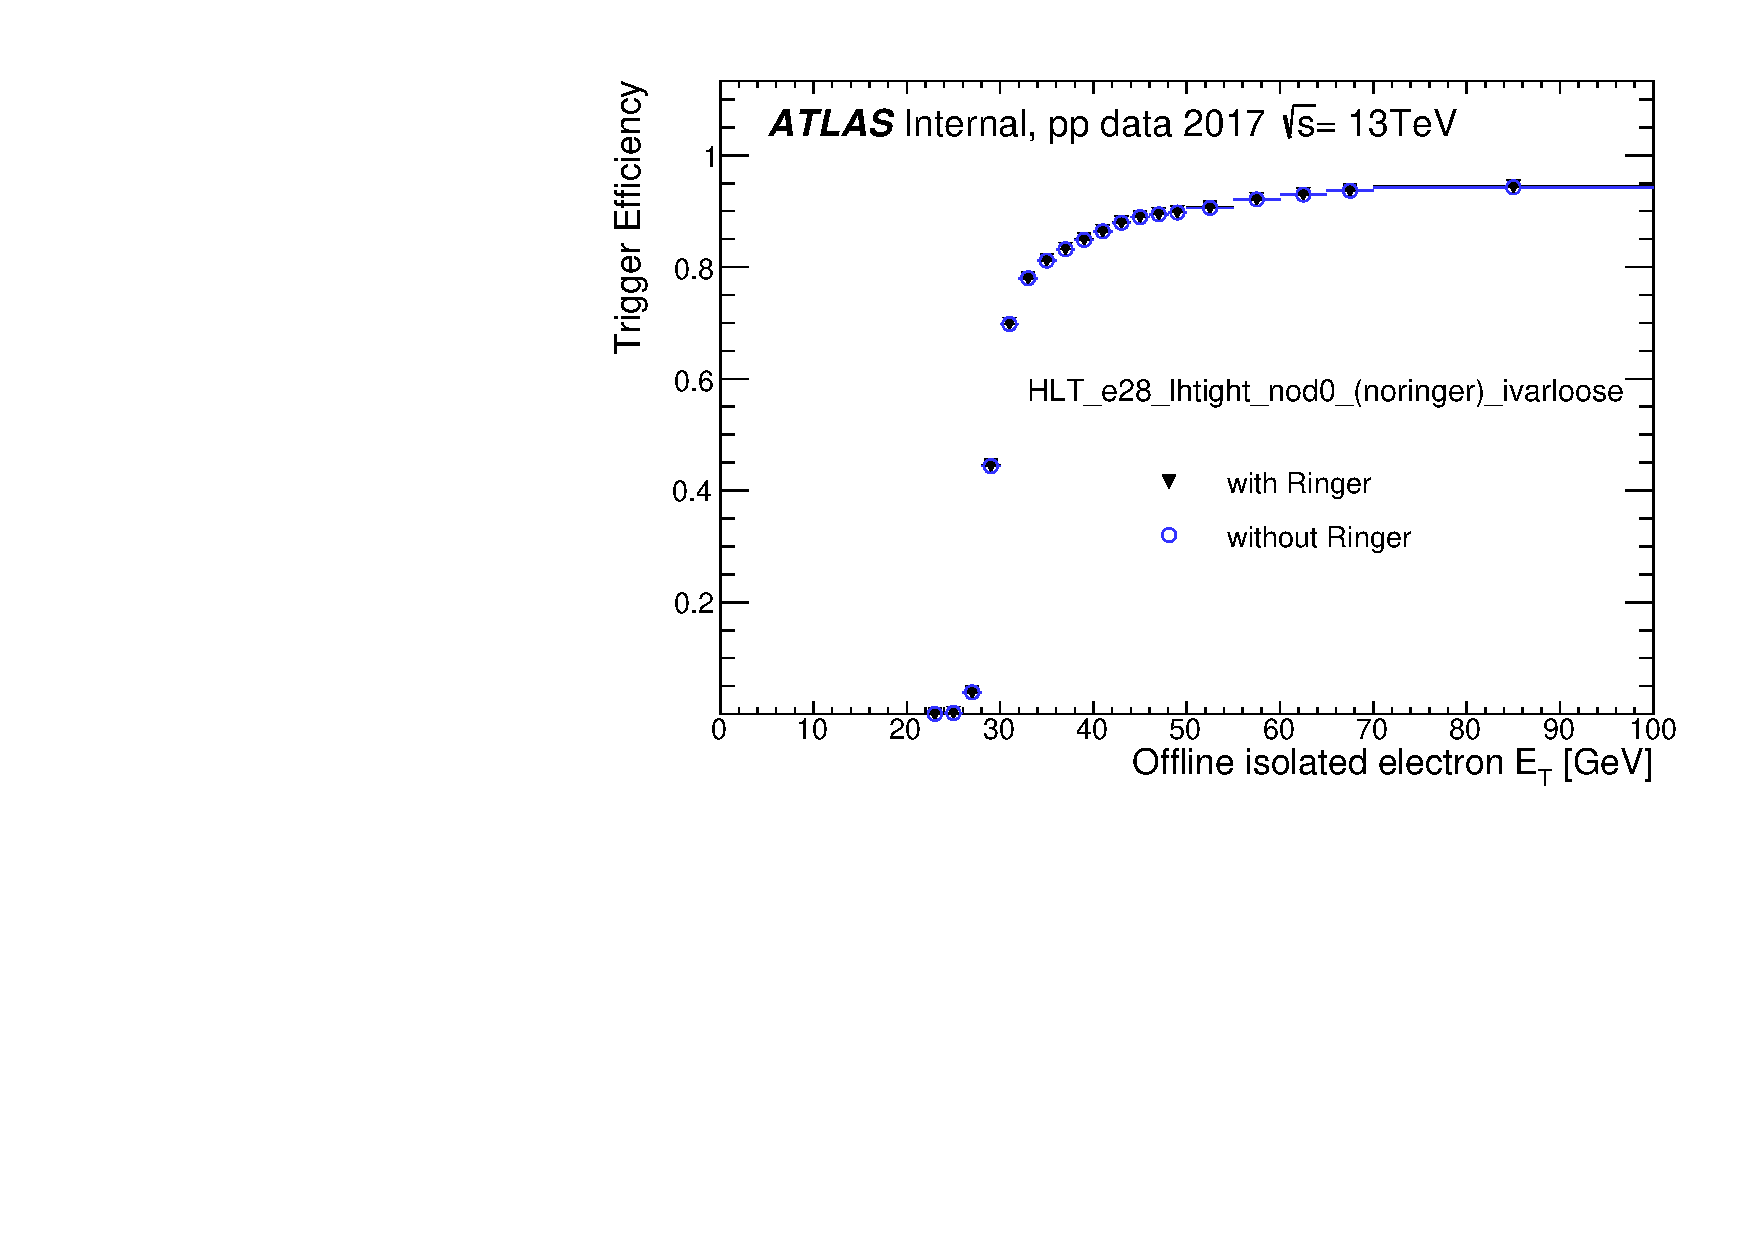
\includegraphics[width=\textwidth]{sections/03_operation/figures/efficiencies/eff_EGAM1_e28_ringer_and_noringer_2017_after_ts1_HLT_et.pdf}
  \caption{}
  \end{subfigure}
  %
  \begin{subfigure}[c]{.49\textwidth}
  \centering
  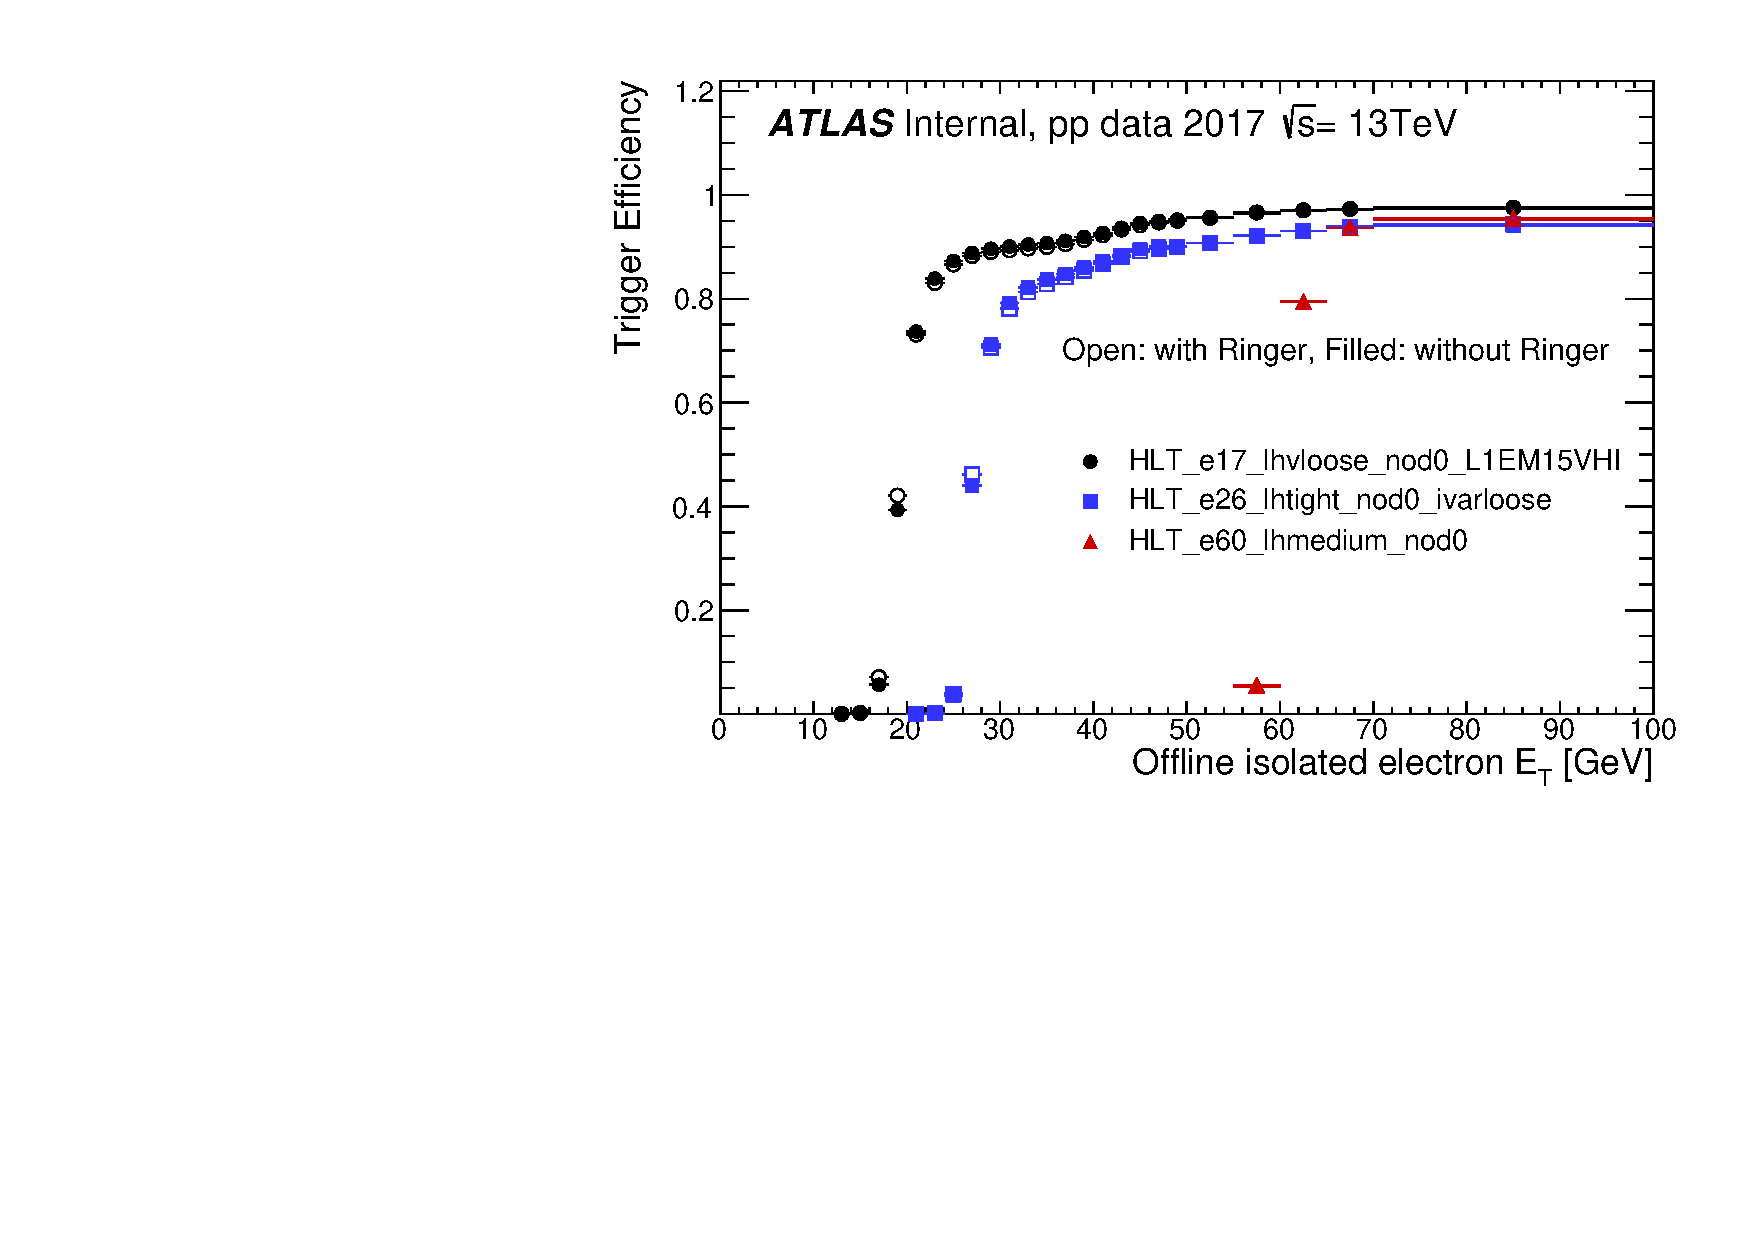
\includegraphics[width=\textwidth]{sections/03_operation/figures/efficiencies/eff_EGAM1_e17_e26_e60_2017_before_and_after_ts1_et.pdf}
  \caption{}%
  \end{subfigure}\\
  %
  \begin{subfigure}[c]{.49\textwidth}
  \centering
  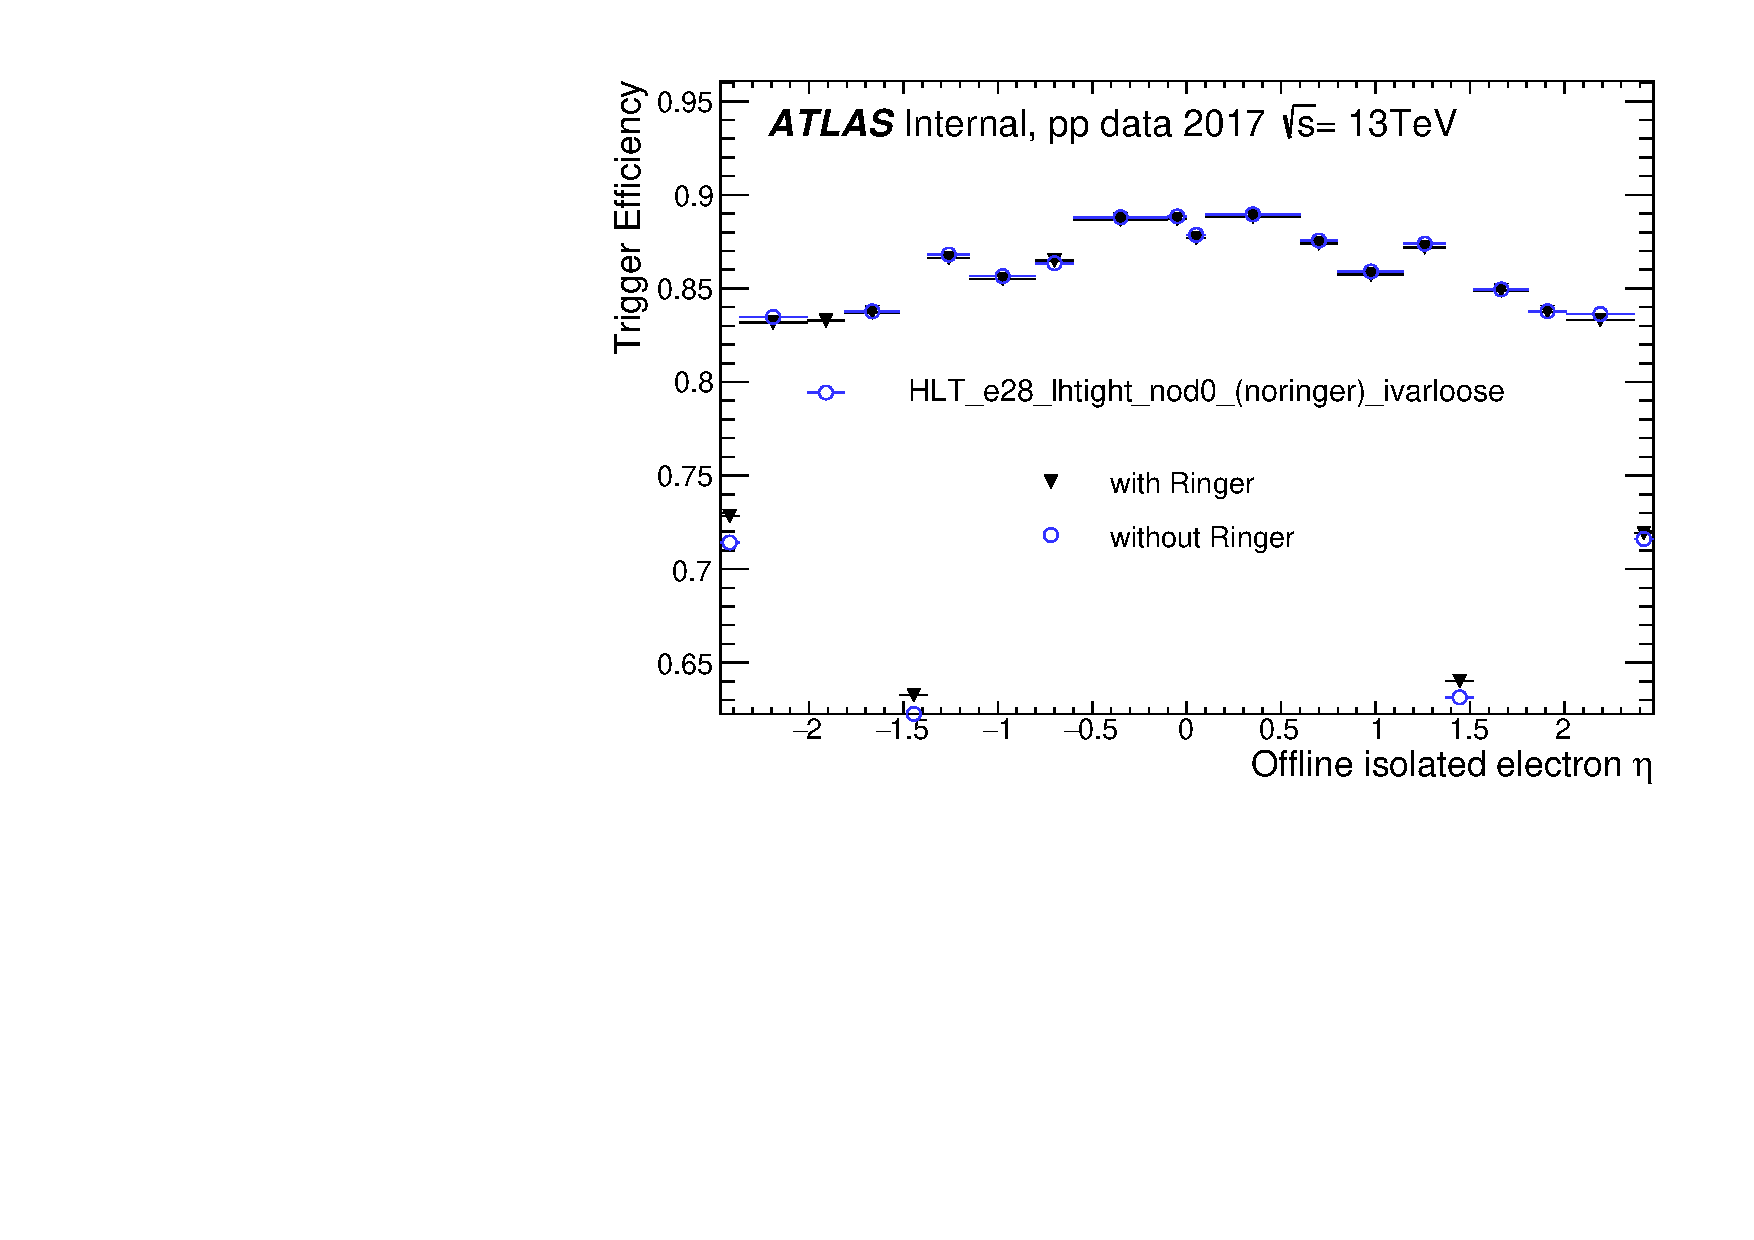
\includegraphics[width=\textwidth]{sections/03_operation/figures/efficiencies/eff_EGAM1_e28_ringer_and_noringer_2017_after_ts1_HLT_eta.pdf}
  \caption{}
  \end{subfigure}
  %
  \begin{subfigure}[c]{.49\textwidth}
  \centering
  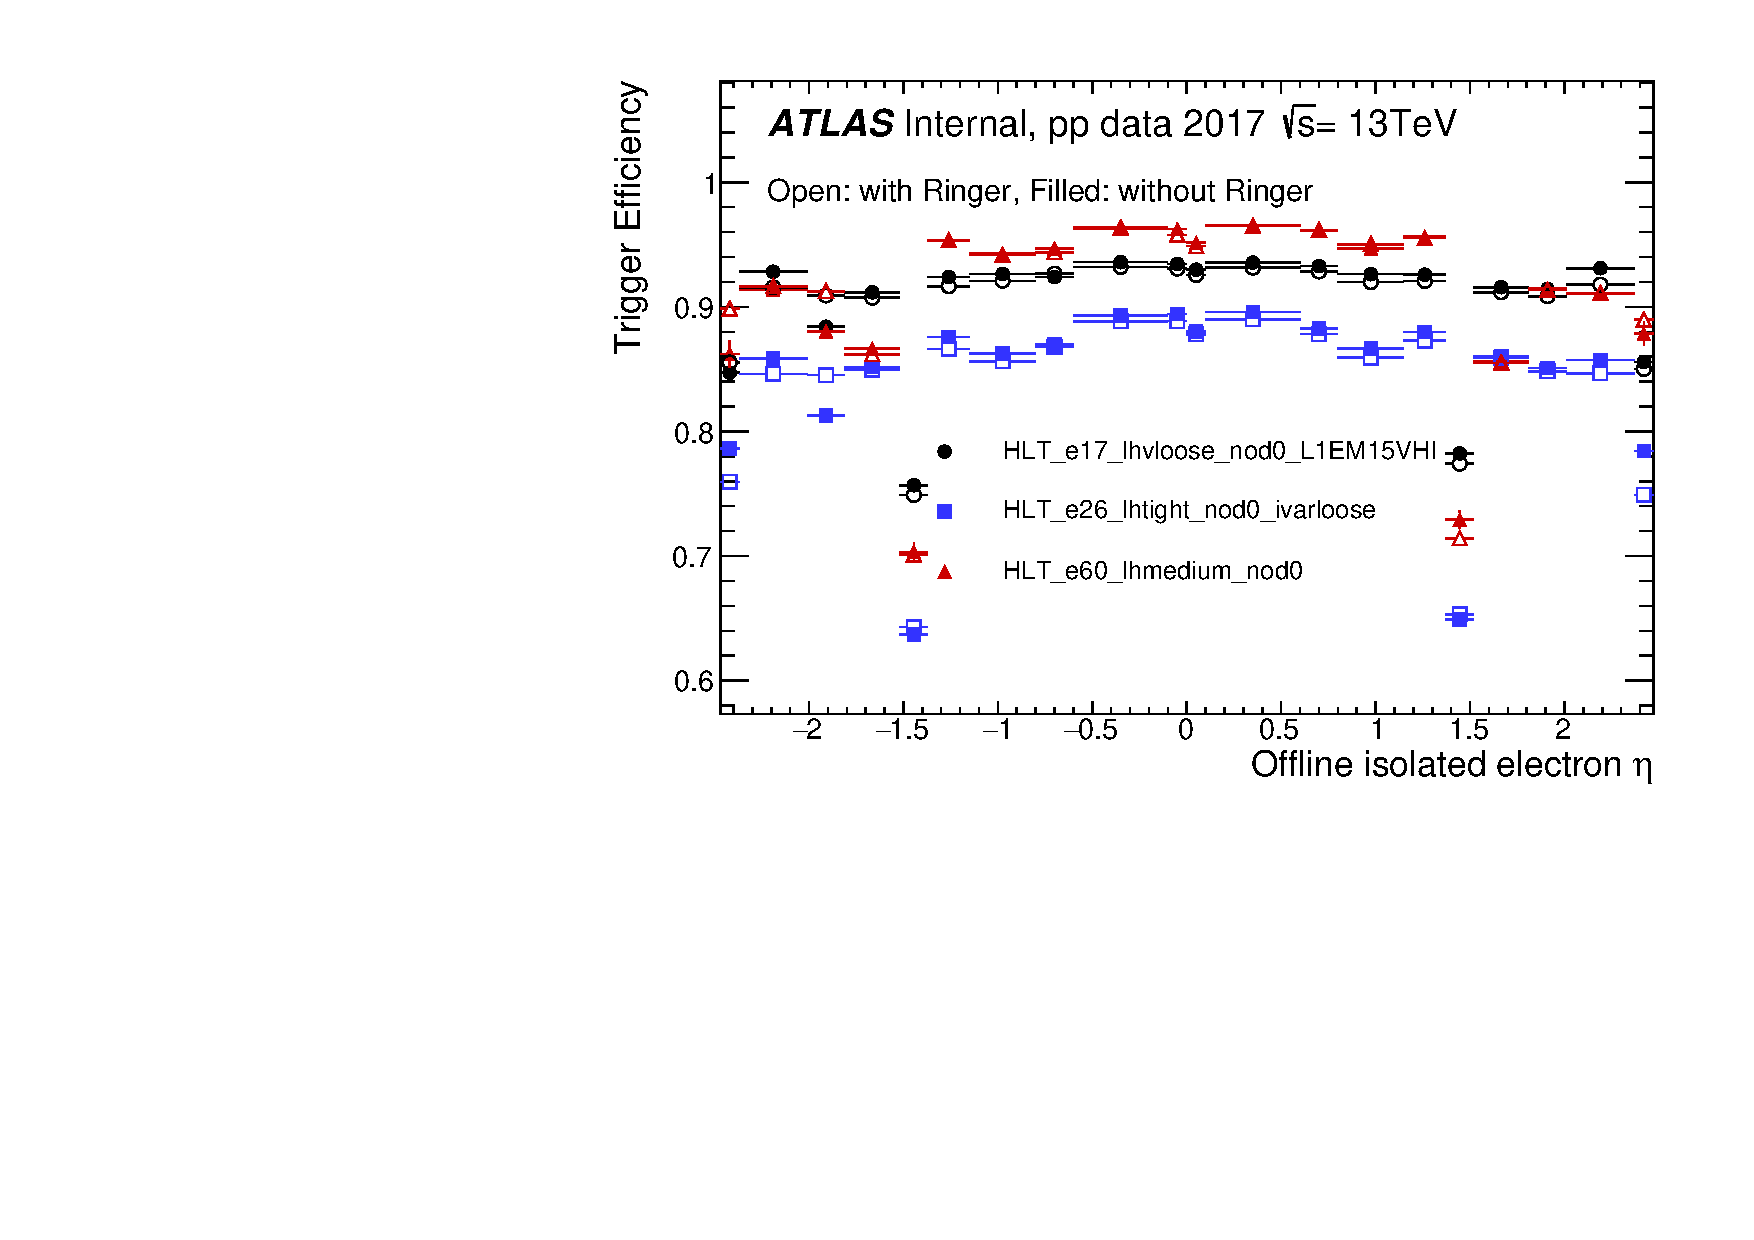
\includegraphics[width=\textwidth]{sections/03_operation/figures/efficiencies/eff_EGAM1_e17_e26_e60_2017_before_and_after_ts1_eta.pdf}
  \caption{}%
  \end{subfigure} \\
  %
  \begin{subfigure}[c]{.49\textwidth}
  \centering
  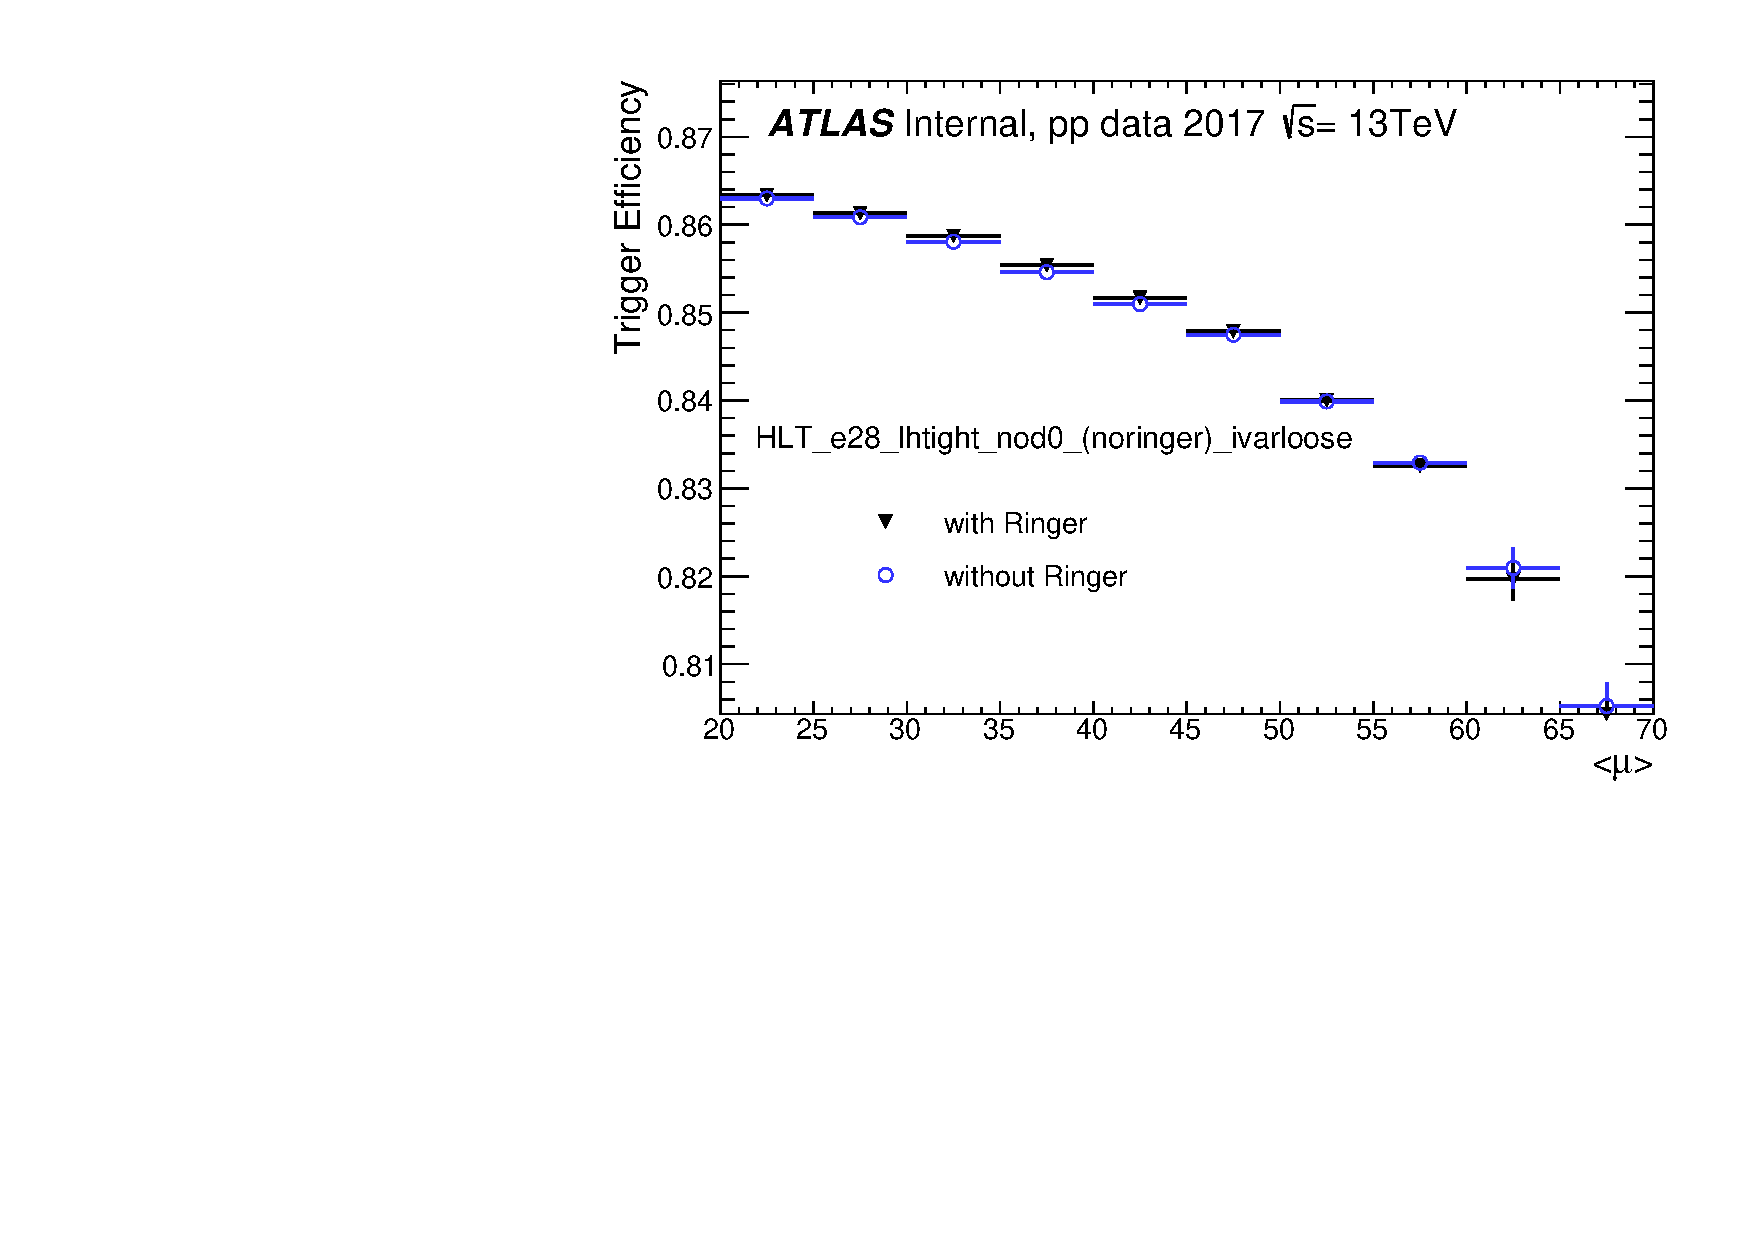
\includegraphics[width=\textwidth]{sections/03_operation/figures/efficiencies/eff_EGAM1_e28_ringer_and_noringer_2017_after_ts1_HLT_mu.pdf}
  \caption{}%
  \label{fig:e28_comp_mu}
  \end{subfigure}
  %
  \begin{subfigure}[c]{.49\textwidth}
  \centering
  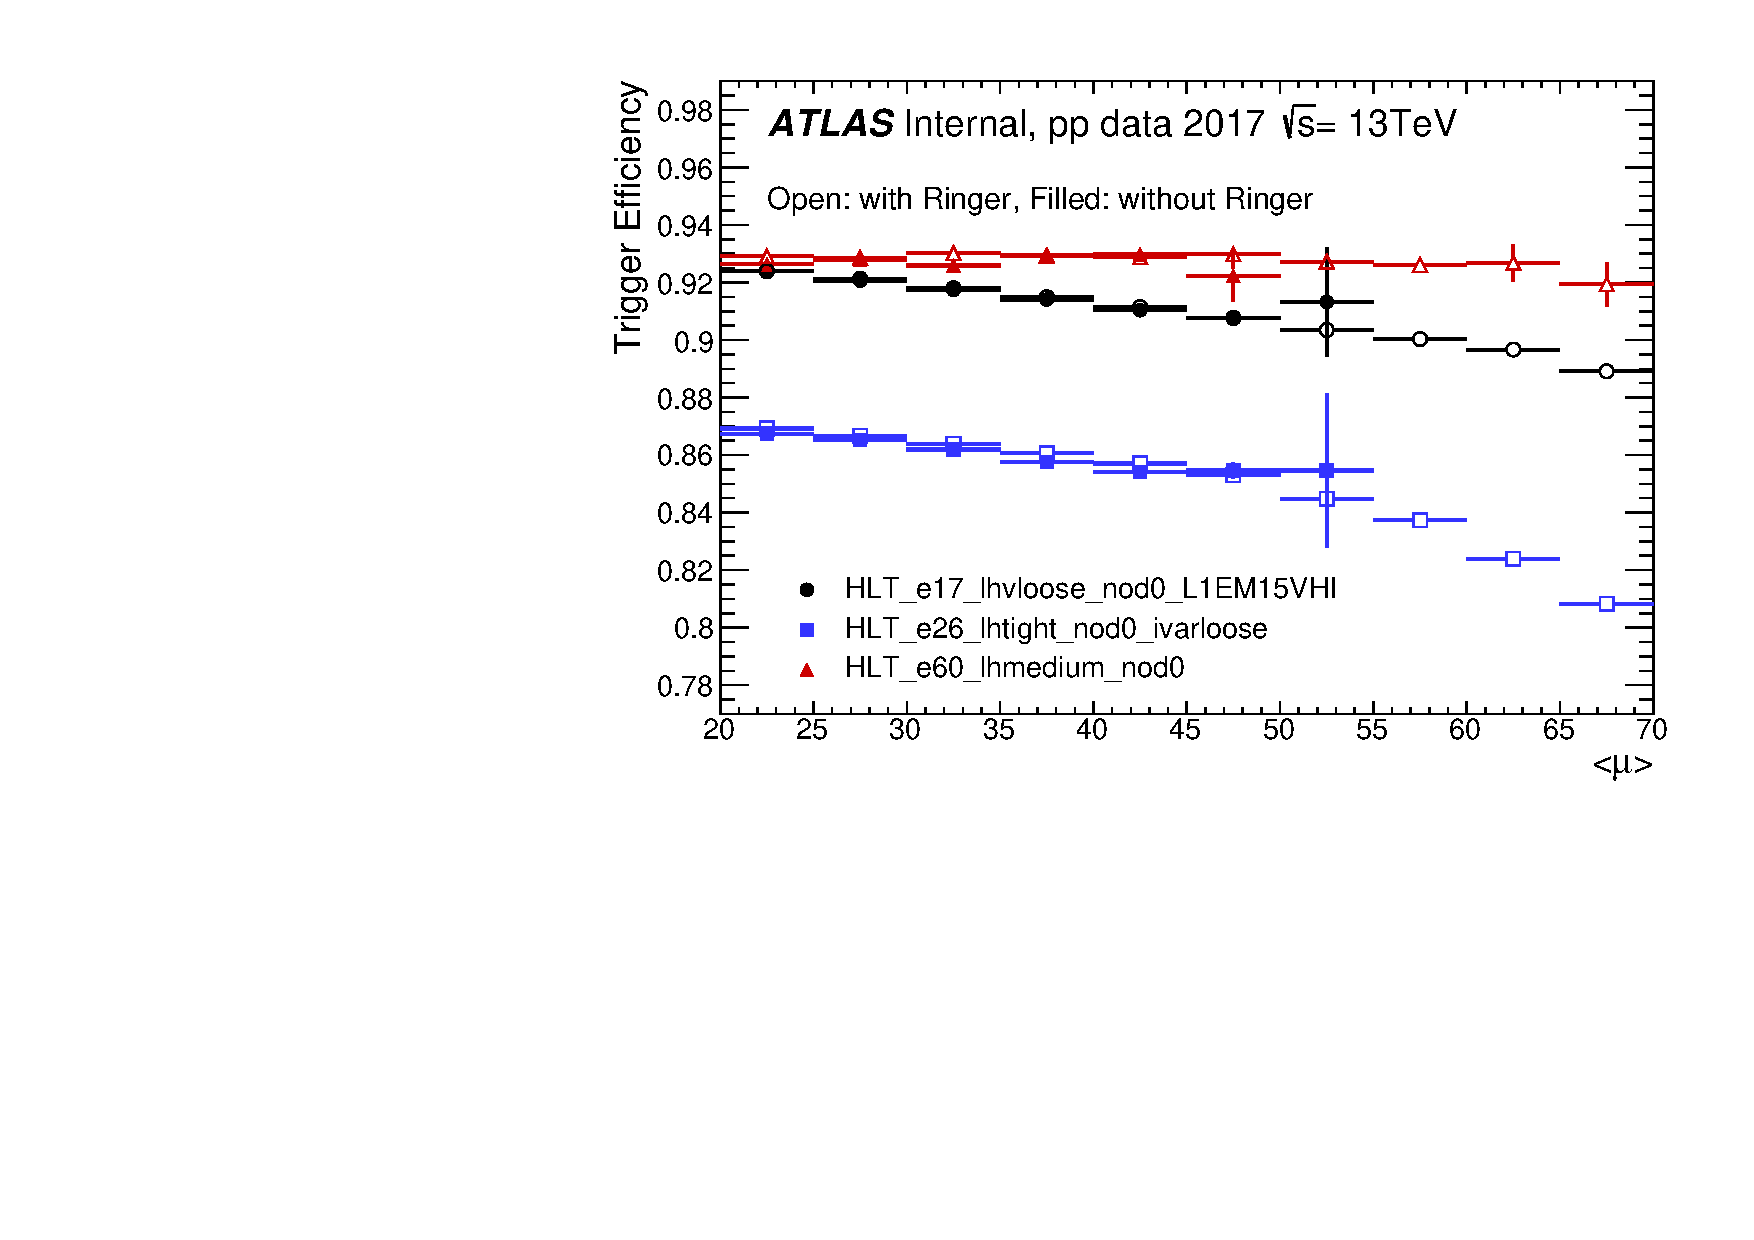
\includegraphics[width=\textwidth]{sections/03_operation/figures/efficiencies/eff_EGAM1_e17_e26_e60_2017_before_and_after_ts1_mu.pdf}
  \caption{}%
  \end{subfigure}
  
  \caption{Left: HLT electron efficiency as a function of \et{} (a), \eta{} (c) and \avgmu{} (e) for the single electron isolated trigger requiring $\et{} > \SI{28}{\GeV}$ and \tight{} selection with and without the \rnn{} algorithm employing 2017 collision data. Right: Efficiency of three single electron triggers as a function of \et (b), \eta (d) and \avgmu (f) for 2017 collision data. Open (closed) markers contain the efficiency measurements on runs before (after) the deployment of the \rnn{}, thus referring to triggers being executed without (with) the \rnn{} algorithm. For 2017 collision data, the higher \avgmu{} values were reached only after the deployment.}
  \label{fig:2017_zee_triggers}
\end{figure}




By contrasting the behavior of the duplicated trigger using fake electron collision data, it becomes clear the power of the \rnn{} algorithm. An overall reduction factor of
the fake rate by a factor of 13.75 is achieved at \fastcalo step. It can be seen in Figure~\ref{fig:2017_fake_triggers} left size, that the improvement at \fastcalo is similar for all
regions in the evaluated variables, particularly interesting when
considering the low \et{} and the end-cap regions. Besides the capability of improving early fake rejection, the usage of the \rnn{} also contributed to reduce the final fake rate at HLT step
(Figure~\ref{fig:2017_fake_triggers} right size) by a factor of 2, mostly coming from the transition regions in the calorimeter.



\begin{figure}[h!tb]
  \begin{subfigure}[c]{.49\textwidth}
  \centering
  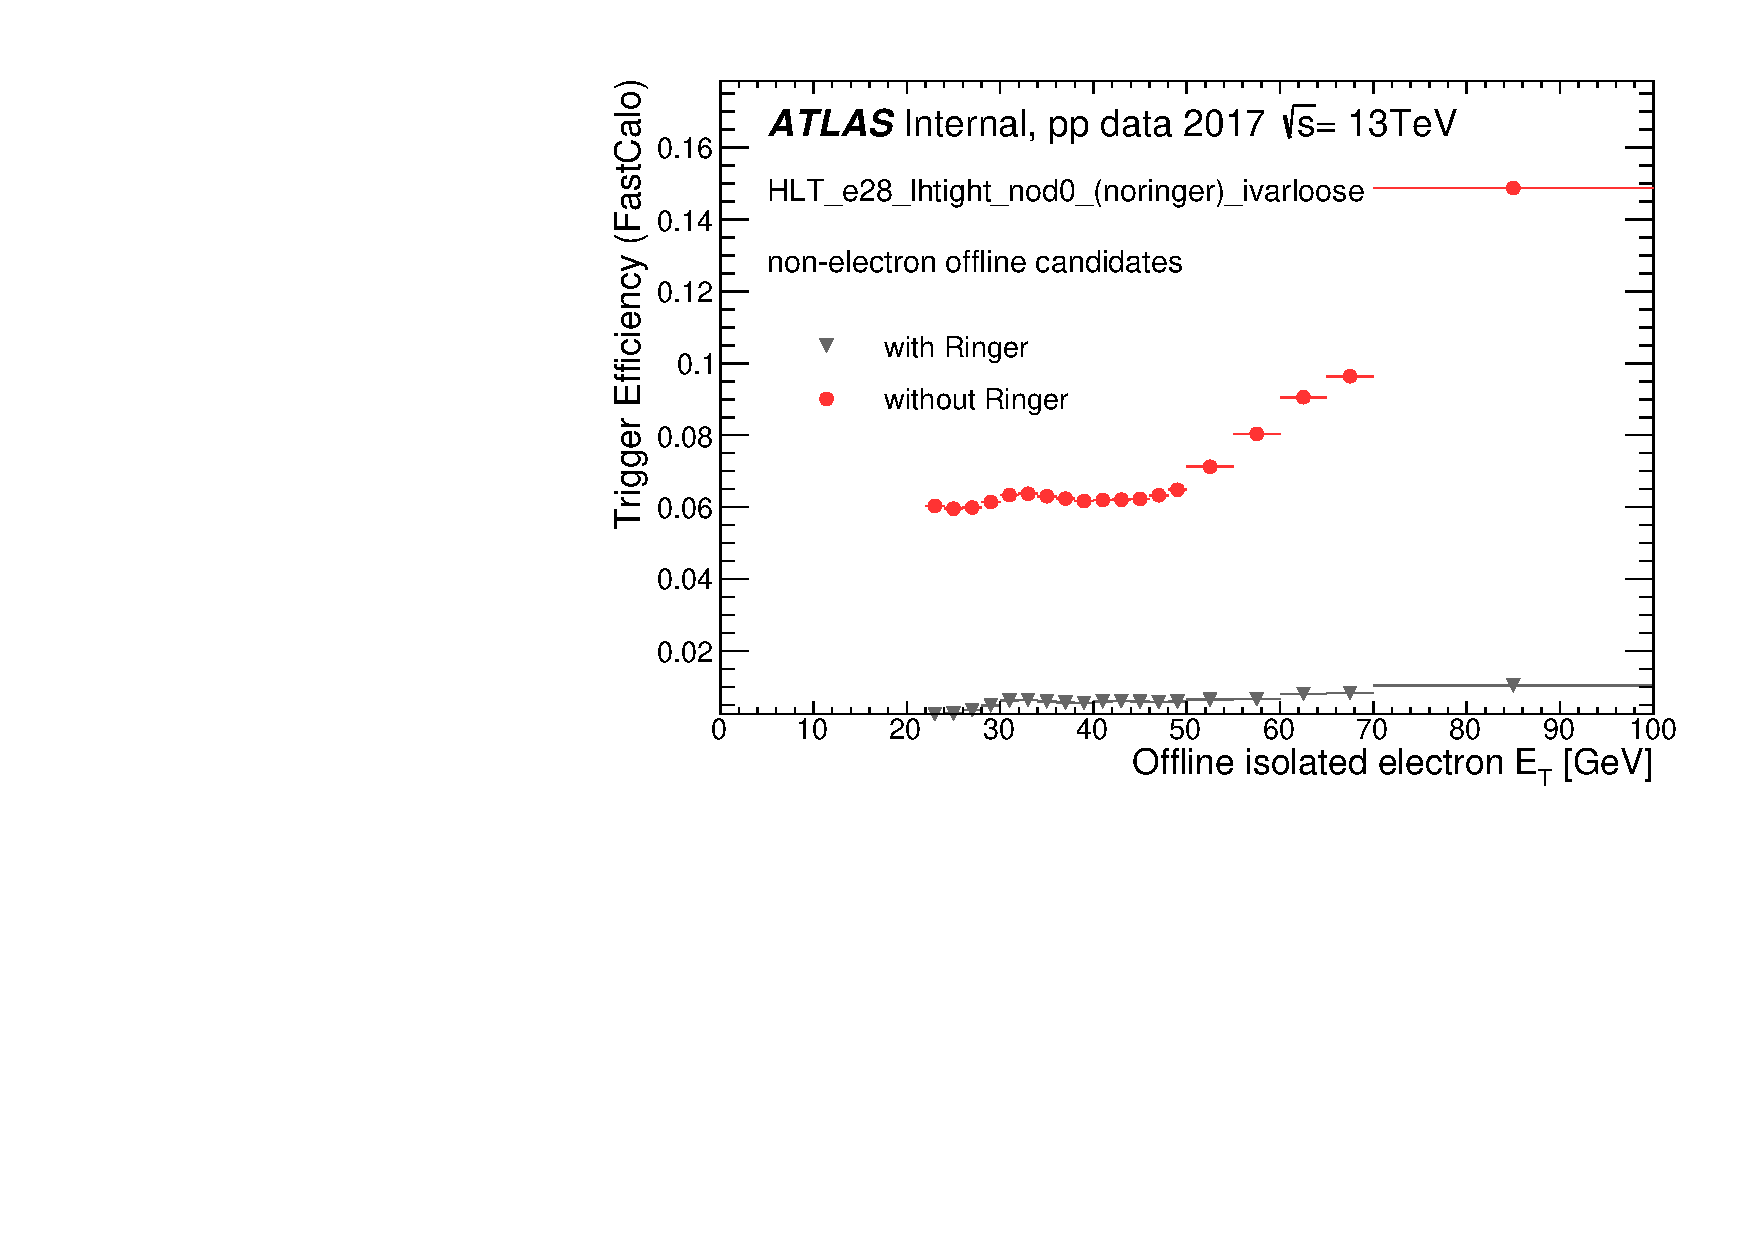
\includegraphics[width=\textwidth]{sections/03_operation/figures/efficiencies/eff_EGAM7_e28_ringer_and_noringer_2017_after_ts1_L2Calo_et.pdf}
  \caption{}
  \end{subfigure}
  %
  \begin{subfigure}[c]{.49\textwidth}
  \centering
  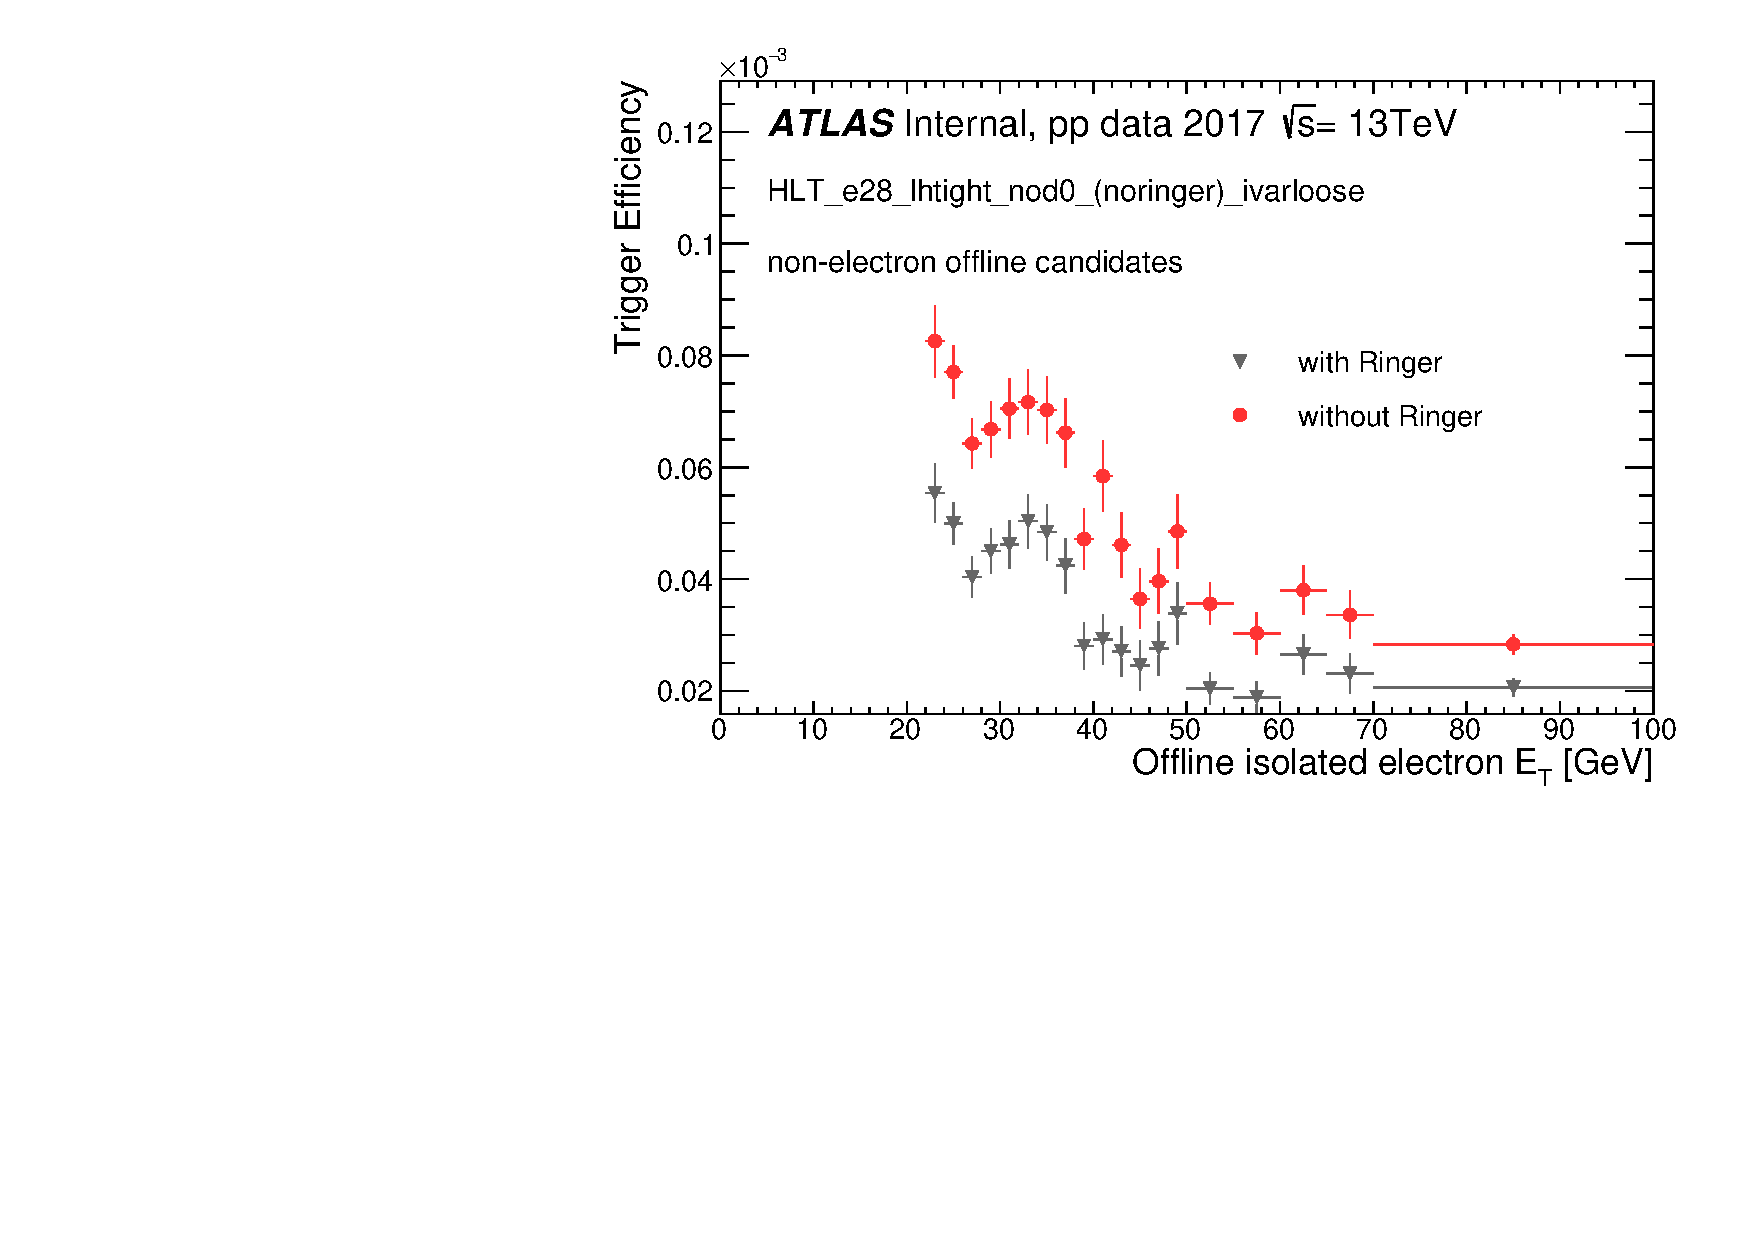
\includegraphics[width=\textwidth]{sections/03_operation/figures/efficiencies/eff_EGAM7_e28_ringer_and_noringer_2017_after_ts1_et.pdf}
  \caption{}
  \end{subfigure}\\
  %
  \begin{subfigure}[c]{.49\textwidth}
  \centering
  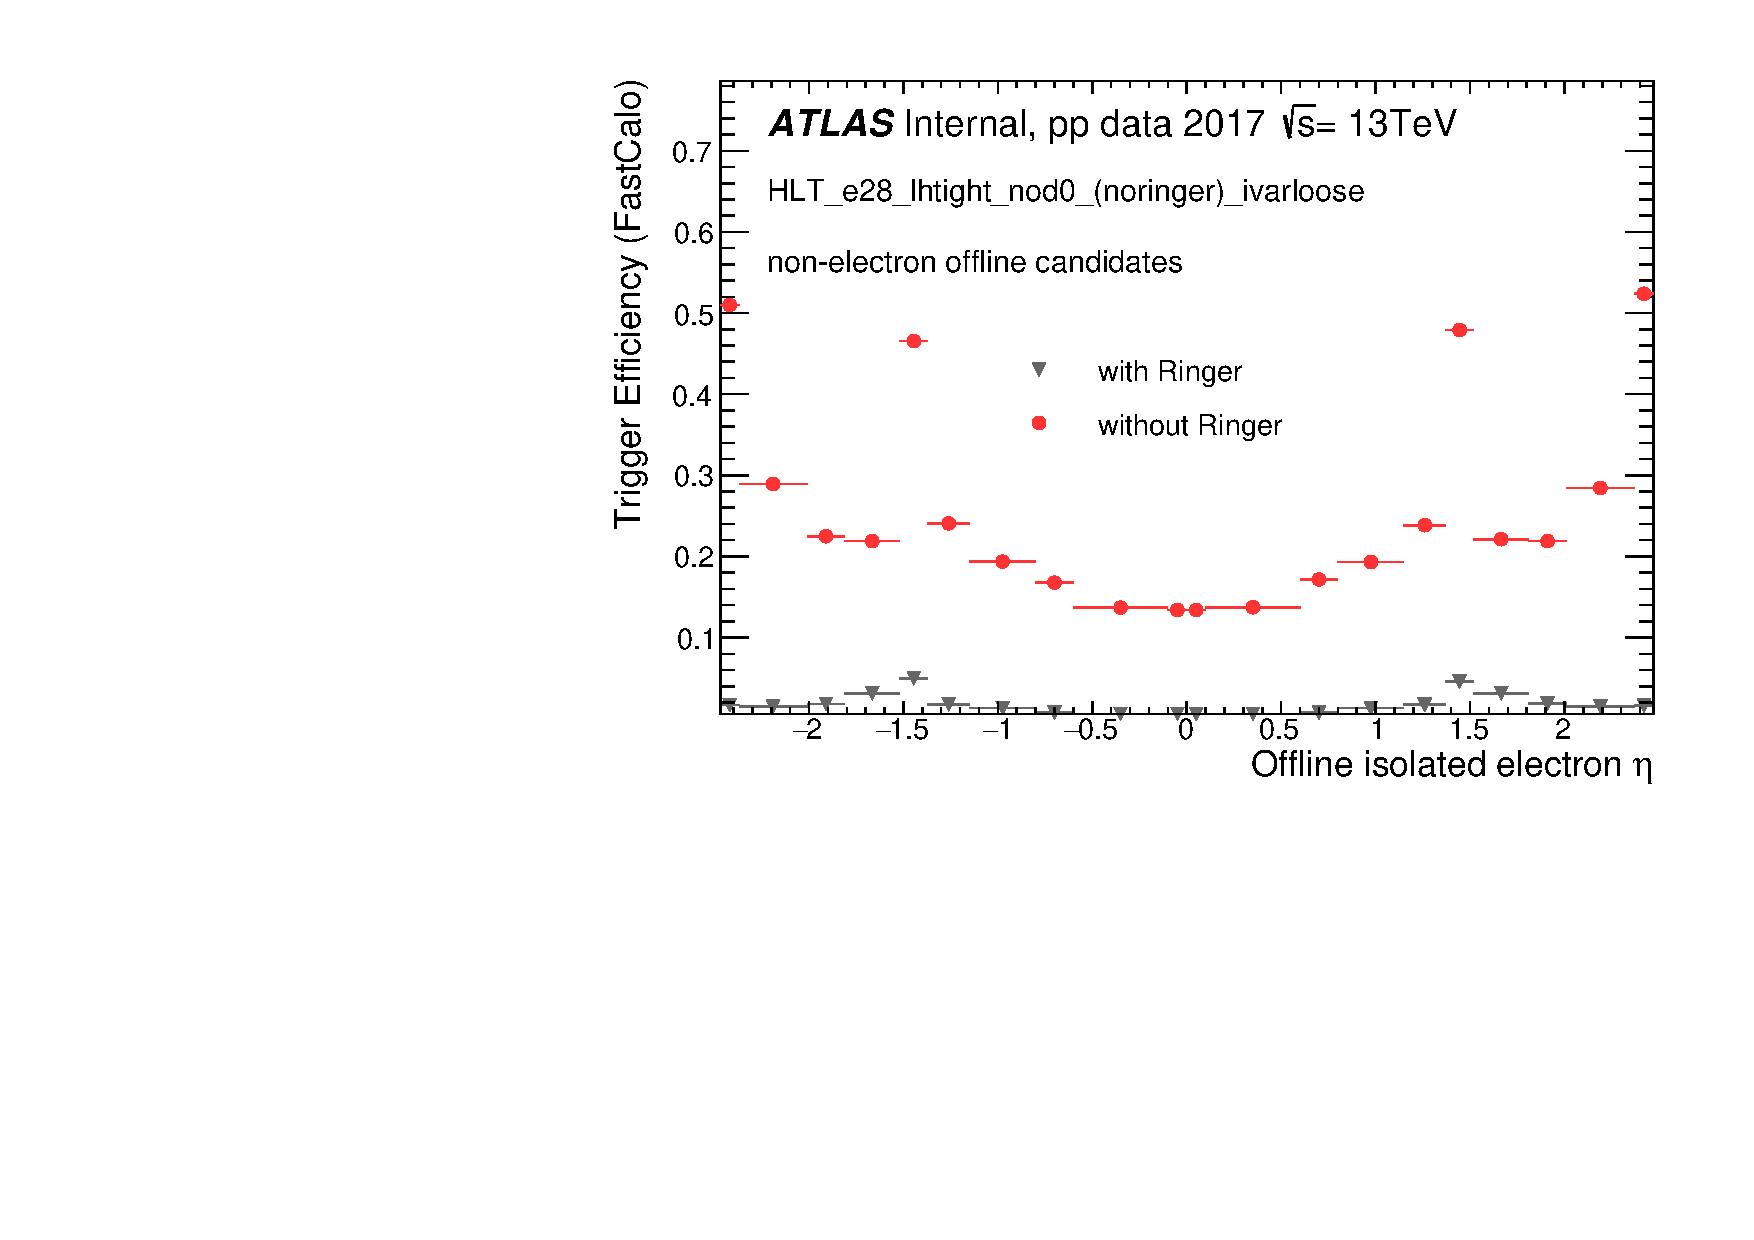
\includegraphics[width=\textwidth]{sections/03_operation/figures/efficiencies/eff_EGAM7_e28_ringer_and_noringer_2017_after_ts1_L2Calo_eta.pdf}
  \caption{}
  \end{subfigure}
  %
  \begin{subfigure}[c]{.49\textwidth}
  \centering
  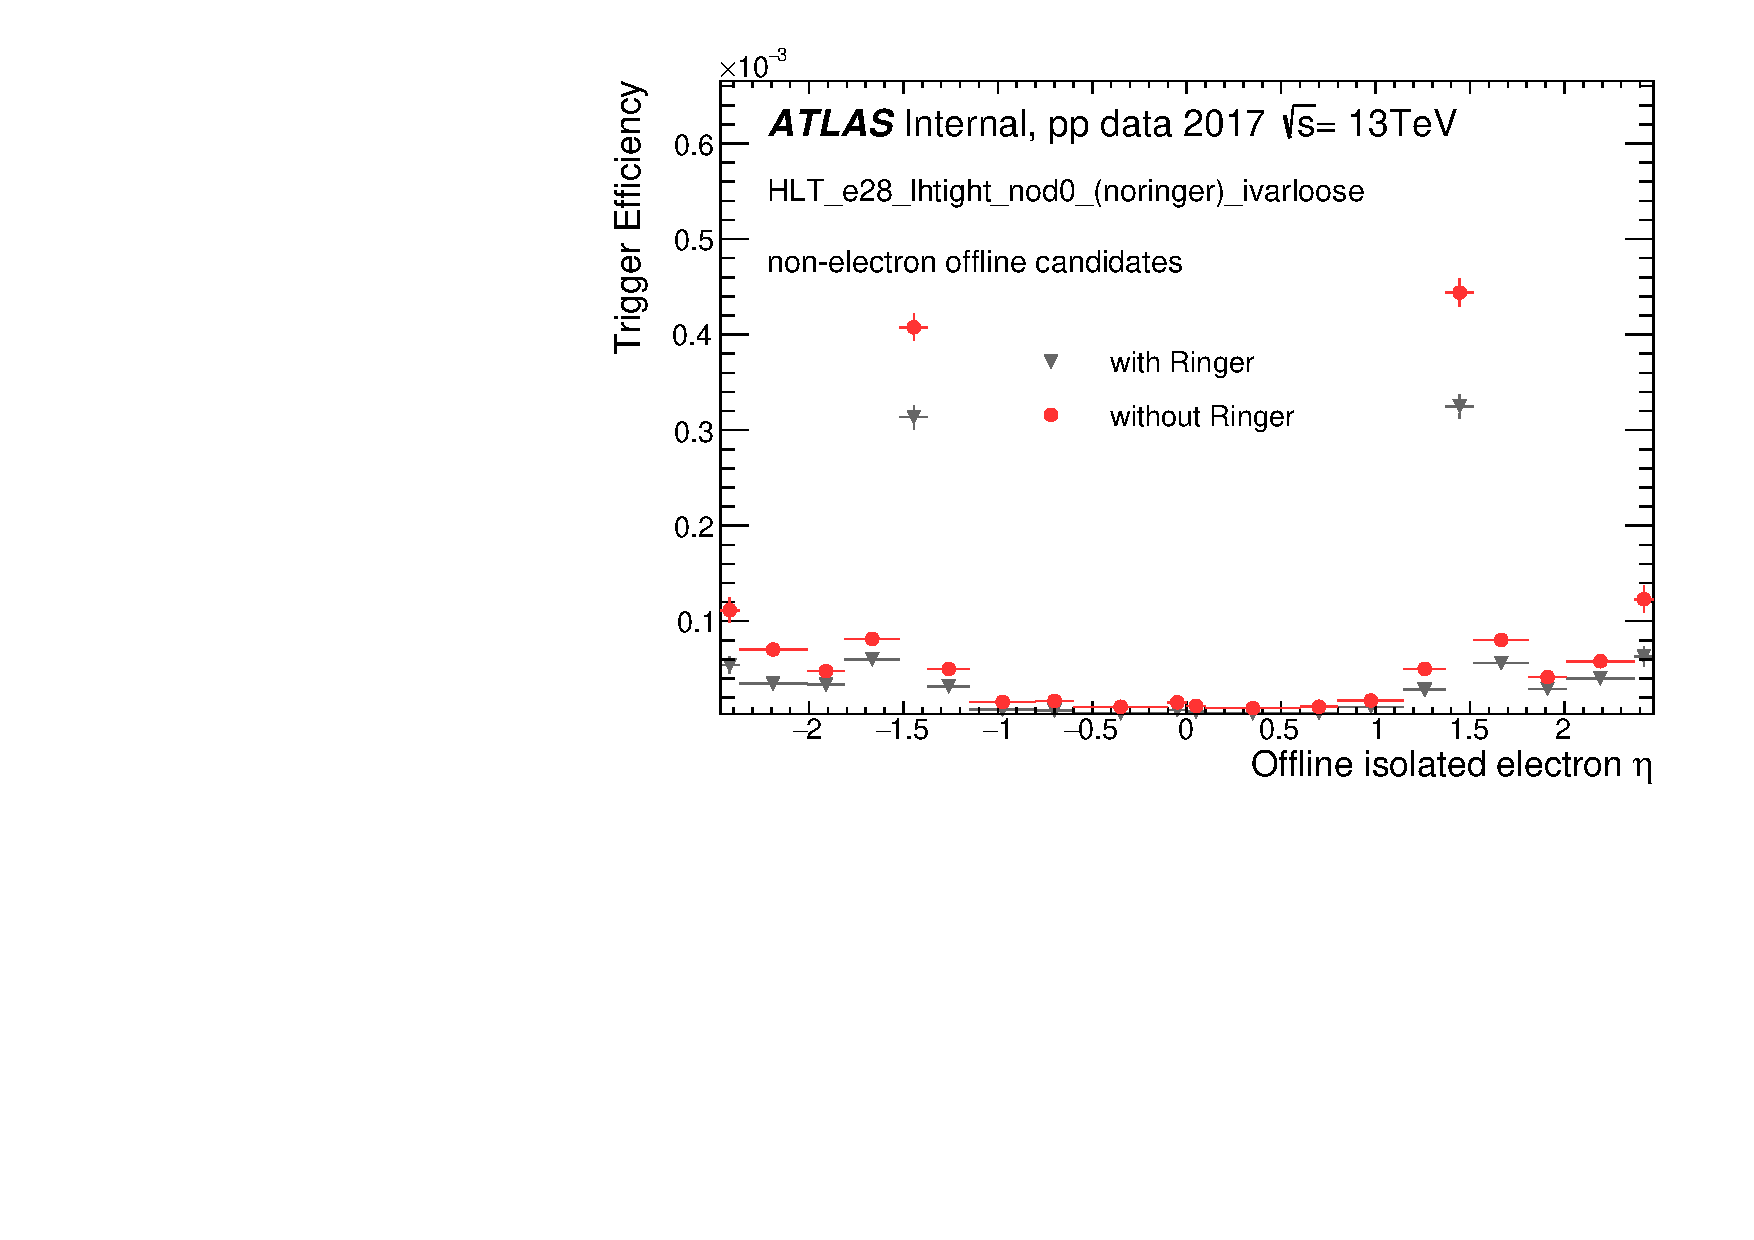
\includegraphics[width=\textwidth]{sections/03_operation/figures/efficiencies/eff_EGAM7_e28_ringer_and_noringer_2017_after_ts1_eta.pdf}
  \caption{}
  \end{subfigure}\\
  %
  \begin{subfigure}[c]{.49\textwidth}
  \centering
  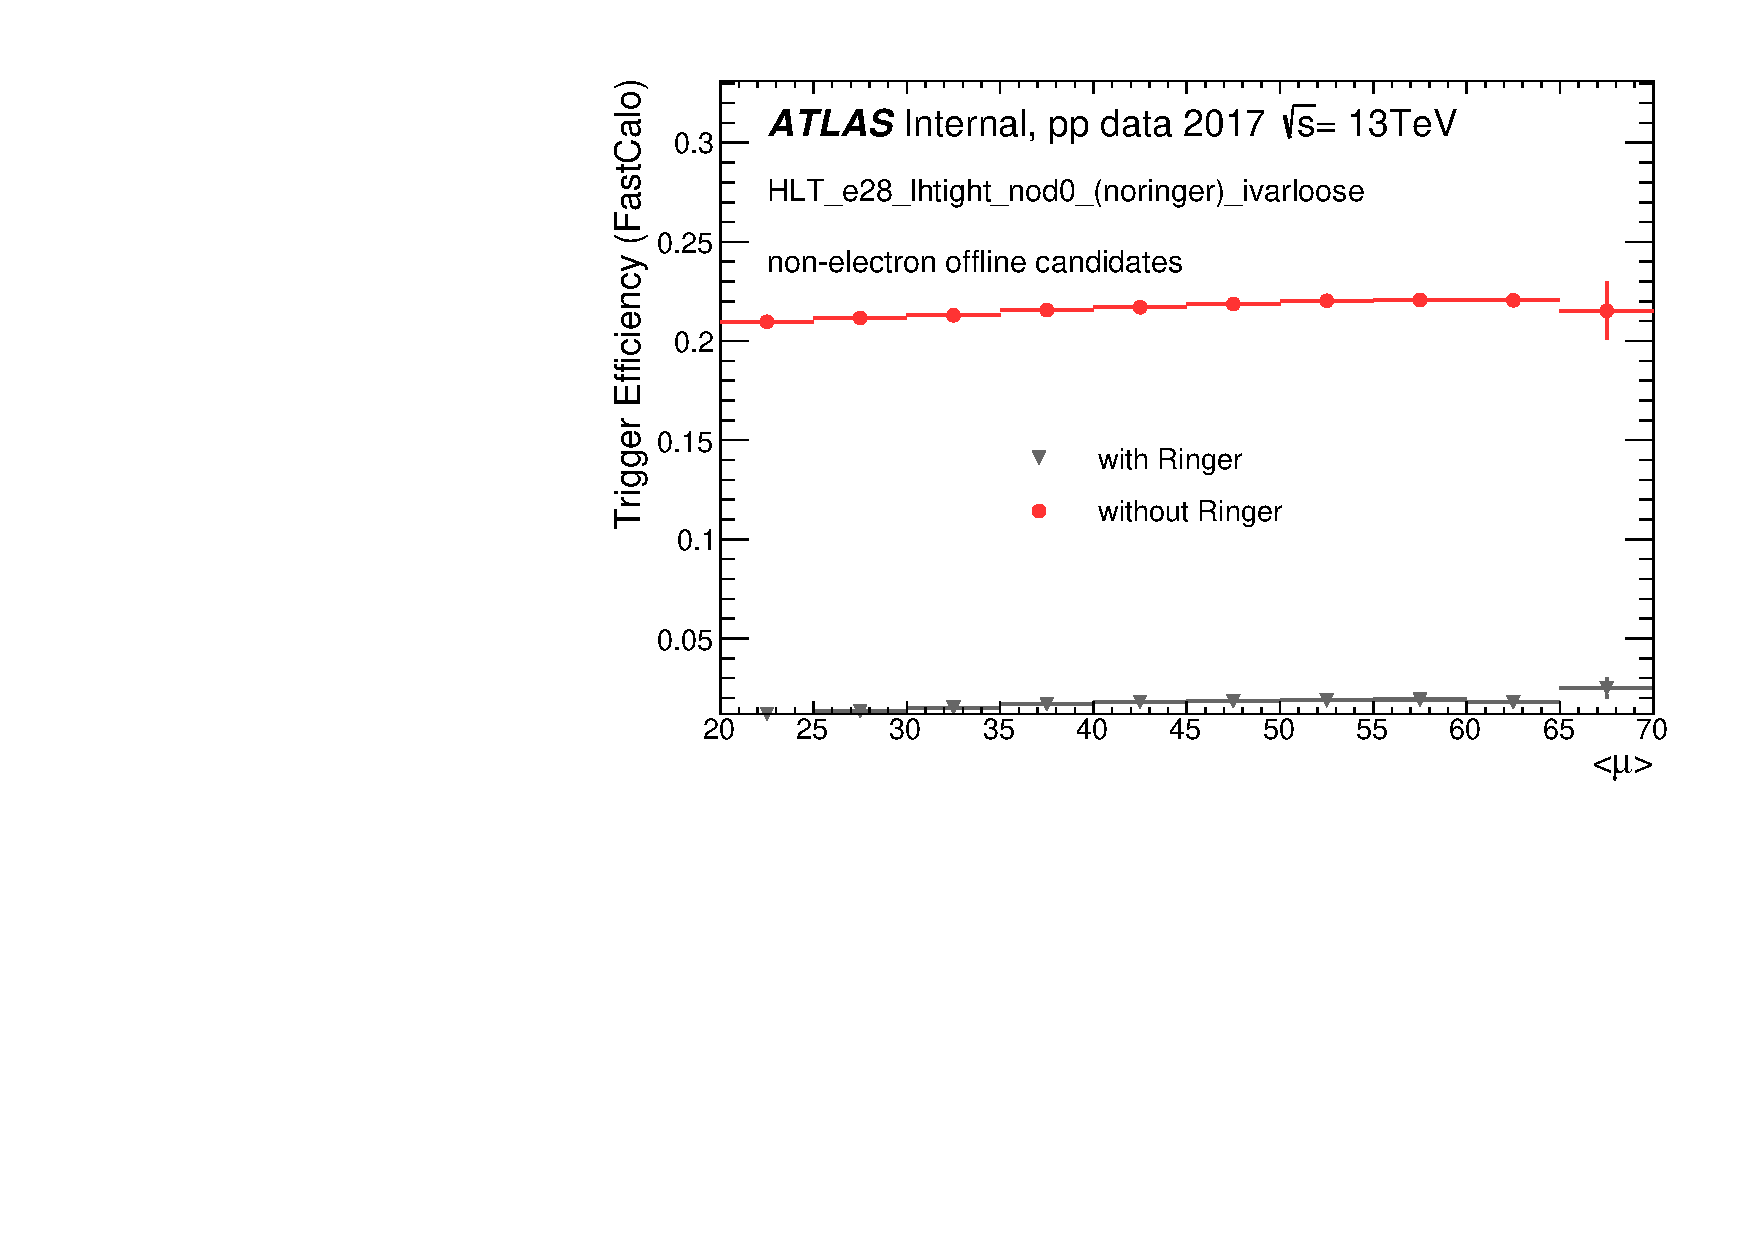
\includegraphics[width=\textwidth]{sections/03_operation/figures/efficiencies/eff_EGAM7_e28_ringer_and_noringer_2017_after_ts1_L2Calo_mu.pdf}
  \caption{}
  \end{subfigure}
  %
  \begin{subfigure}[c]{.49\textwidth}
  \centering
  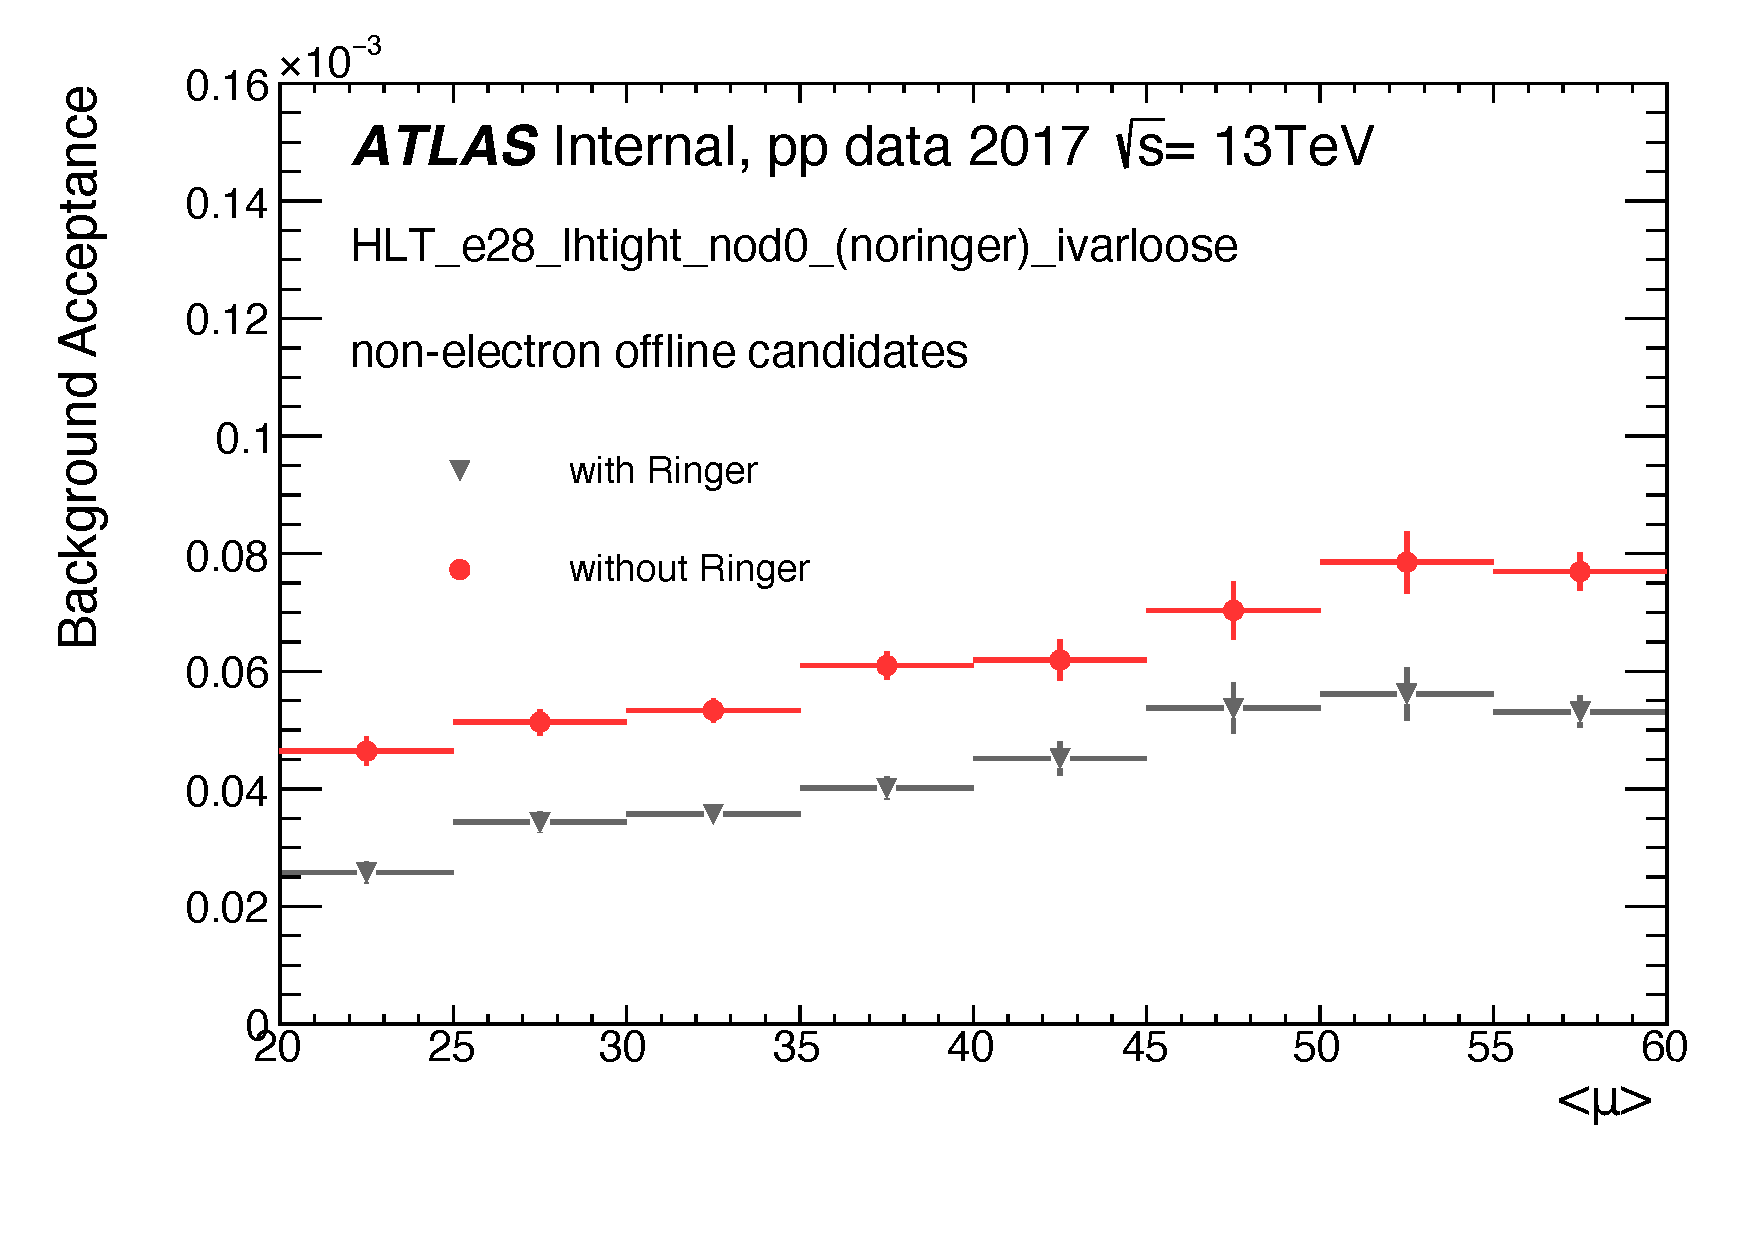
\includegraphics[width=\textwidth]{sections/03_operation/figures/efficiencies/eff_EGAM7_e28_ringer_and_noringer_2017_after_ts1_mu.pdf}
  \caption{}
  \end{subfigure}

  \caption{ Fake electron efficiency as a function for the single electron isolated trigger requiring $\et > \SI{28}{\GeV}$ and \tight selection with and without the \rnn{} algorithm employing 2017 collision data collected after the \rnn algorithm deployment. Left: \fastcalo fake electron efficiency as a function of \et (a), \eta (c) and \avgmu (e). Right: HLT fake electron efficiency as a function of \et (b), \eta (d) and \avgmu (f).}%
  \label{fig:2017_fake_triggers}
\end{figure}




\subsection{2018 Operation}\label{ssec:2018_ringer_operation}

In 2018, the \rnn{} operated with a new tune based on collision data. It was also the case for the final HLT
selection\footnote{One exception was the \medium{} selection, where the HLT likelihood selection operated in 2018 with the same 2017 tune.}. For the lowest-transverse energy-threshold unprescaled trigger, an efficiency improvement of at least one percentage point in central value is observed when comparing both periods, resulting from a better operation in all selection steps, but, in particular, this is due to improvements from the likelihood tunes in the period.

Despite maintaining high electron efficiency, a small reduction in fake acceptance was observed at the  \fastcalo{} step for some unprescaled triggers in comparison with 2017 after TS1. For the lowest-transverse energy-threshold the fake acceptance was reduced by a factor by 1.19. On the other hand, for the highest-transverse energy trigger, a reduction factor by 1.69 was achieved.




\subsection{Impact on CPU Demands} \label{ssec:cpu_reduction}

As observed in the efficiency measurements during 2017-2018 data taking, the \rnn{} allowed for a more effective \fastcalo{} operation in triggers with electrons above \SI{15}{\GeV}  with respect to the previous cut-based approach. 



The overhead required to compute the NN decision by running a single electron trigger with and without the \rnn algorithm, in two individual non-concurrent executions using the same dedicated node\footnote{It was used a techlab node Xeon Phi 7120 (1.7 GHz, 32 threads) with 256 Gb@1333 of memory and a SL6 OS.}, was evaluated. It should be mentioned that, in order to reduce implementation efforts, electron triggers executing the \rnn{} information compute their information after the cut-based reconstruction, whose decision is not computed. As a result of this, the \rnn{} electron triggers always demand additional \fastcalo processing time.

Figures~\ref{fig:fastcalo_fex_time} and~\ref{fig:fastcalo_hypo_time} show the comparison of the total processing time per call for the feature extraction and hypothesis algorithms in the \fastcalo respectively (See the related \fastcalo gray rectangles and diamonds in Figure~\ref{fig:electron_chain}). The processing time per call does not include the online data preparation time. The measurements were evaluated from a very loose selection electron trigger with individual executions in the same dedicated computer node.


The measurement employed events from the enhanced bias (EB)
stream~\cite{eb_description} typically extracted from one hour acquisition with
a specific trigger menu based only on first level selection and aiming at
collecting about one million background events more likely to be accepted by the
\hlt{}. This behavior is obtained by applying an increased weighting in high-\pt{} region,
and at a output trigger rate of \SI{300}{\hertz}~\cite{eb_specifications} for one hour. Hence, the measurements are performed under pile-up conditions with the execution of the
reconstructed observable algorithm for multiple RoIs in the same bunch-crossing event.


\begin{figure}[h!tb]
	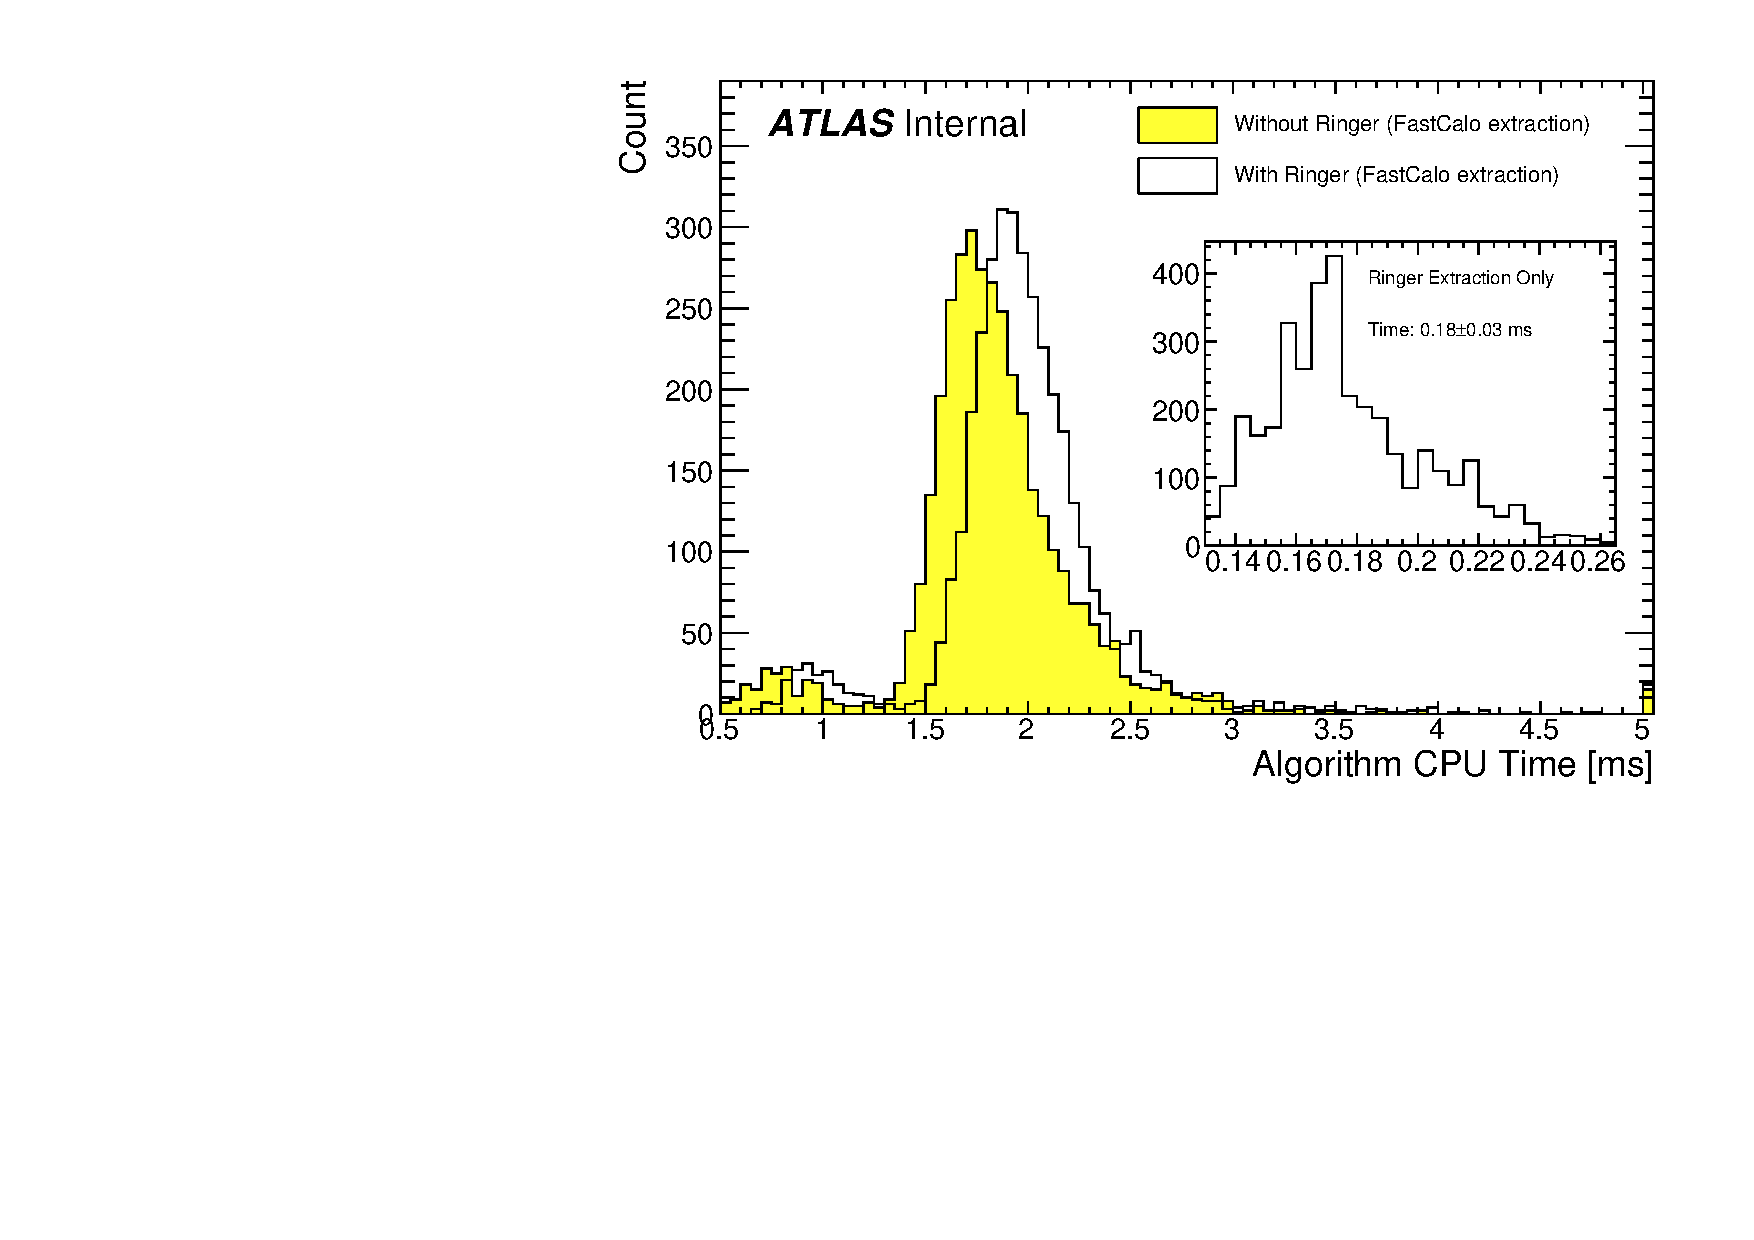
\includegraphics[width=.7\textwidth]{sections/03_operation/figures/EgammaFex_TotalTime}
	\centering
	\caption{\label{fig:fastcalo_fex_time}
		Total processing time per call for the feature extraction algorithms in the \fastcalo step of electron offline rerunning triggers with (white) and without (yellow) \rnn{} using EB events ($\avgmu=45$ peak). Detail on the right shows the individual processing time per call of the ring variable extraction.  
	}
\end{figure}

\begin{figure}[h!tb]
	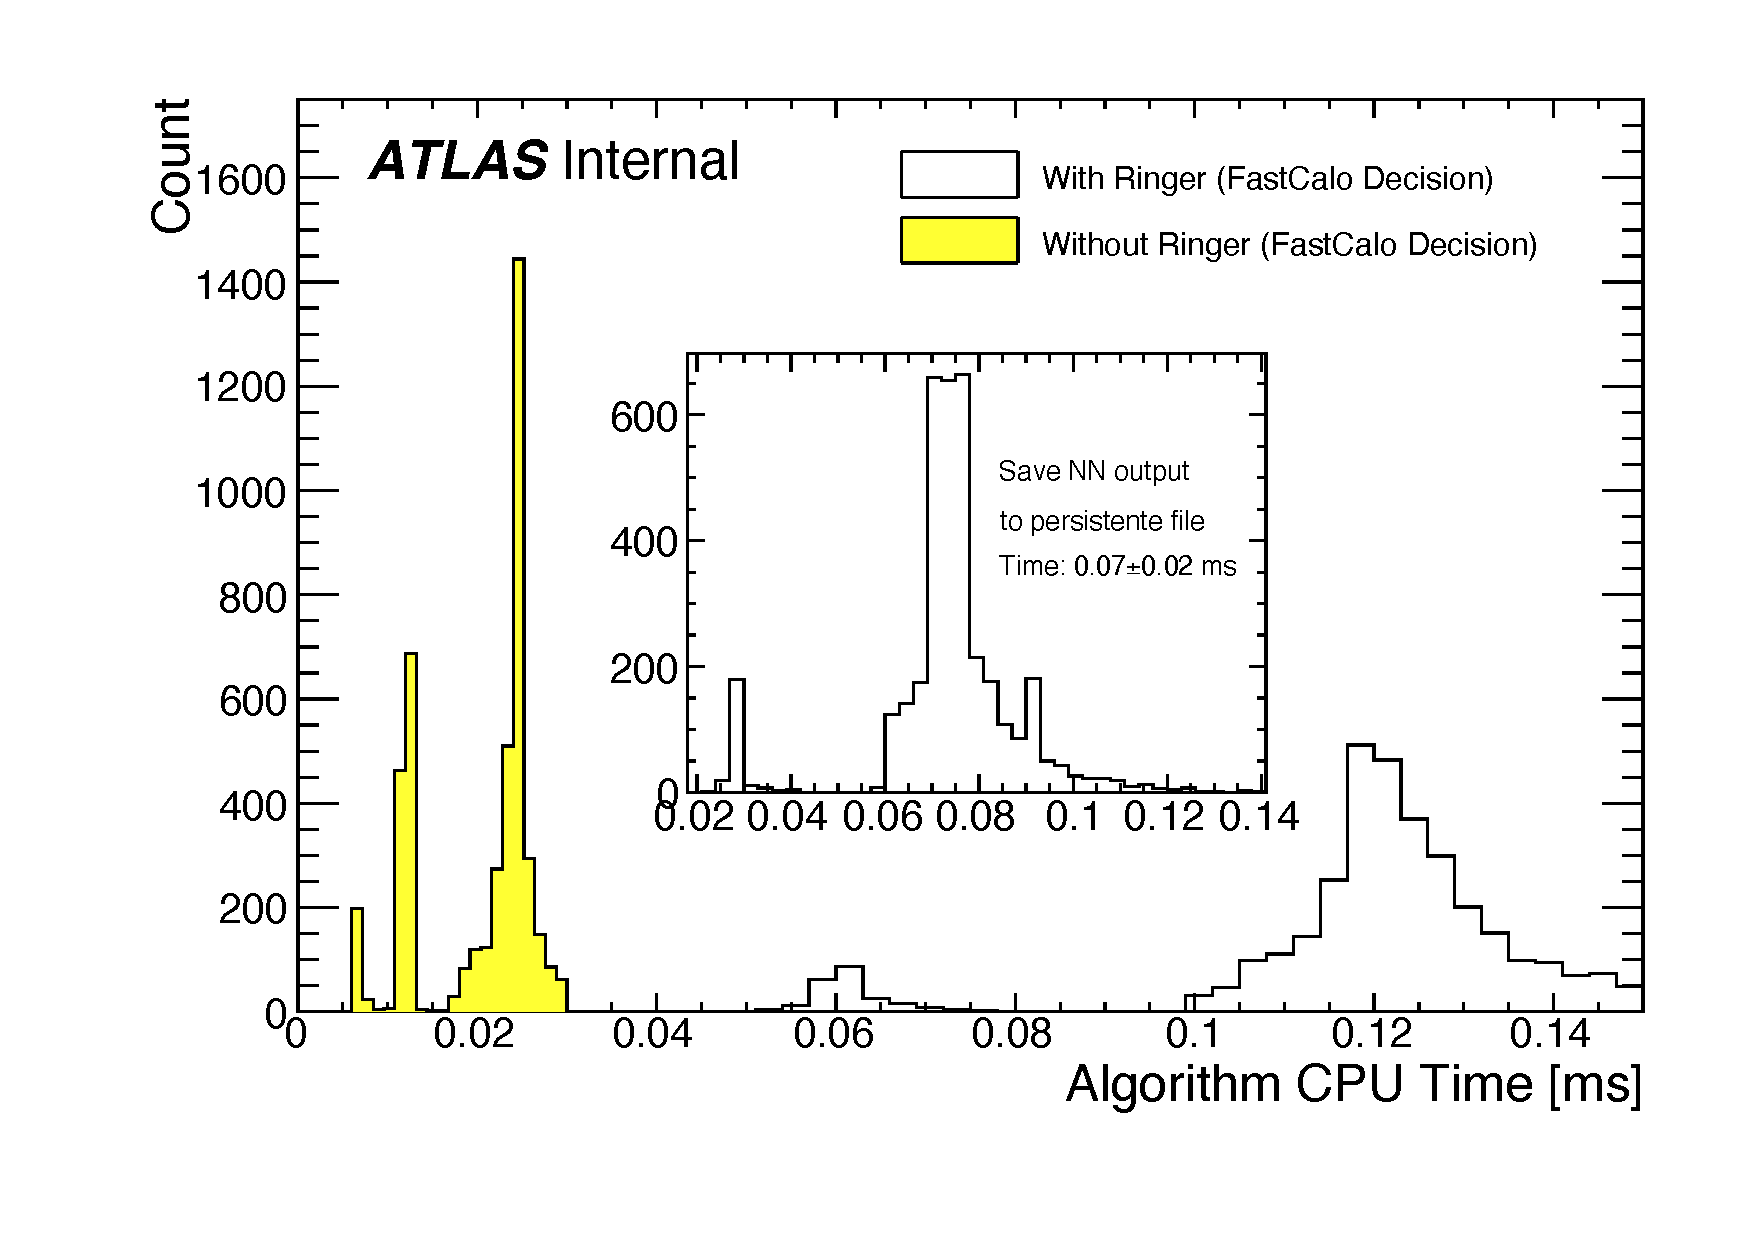
\includegraphics[width=.7\textwidth]{sections/03_operation/figures/EgammaHypo_TotalTime.pdf}
	\centering
	\caption{\label{fig:fastcalo_hypo_time}
		Total processing time per call for the hypothesis testing algorithms
		in the \fastcalo step of electron offline rerunning triggers with (white) and without (yellow) \rnn{} using EB events ($\langle \mu \rangle = 45$ peak). The center histogram represents the individual processing time per call to store the \rnn{} output in persistent file format.}
\end{figure}

A multi-modal structure can be observed in the feature extraction distributions of both trigger configurations, which is associated to the algorithm for retrieving the EM2 cells and building related shower shape
variables\footnote{The three peak structure comes from the raw data conversion. Particularly, these are amongst the most-demanding contributions to the \fastcalo total CPU time.}. The computation of the ring variables, the only difference between the triggers in the \fastcalo feature extraction, requires an additional average processing time of \SI{0.18 \pm 0.03}{\ms/\text{event}}. 


A less relevant contribution comes from hypothesis testing, in which the ring variables are normalized, the discriminating is computed, compared to the selection requirement and stored into the persistent file format\footnote{For Run-3 this step has been removed as a way to reduce the CPU time at \fastcalo step.}. Specifically, \rnn{} hypothesis testing is considerably more demanding, up to \SI{0.14}{\ms/\text{event}}, mostly due to the time 
to store the neural network output \SI{0.07 \pm 0.02}{\ms/\text{event}}, 
than the cut-based selection (\SI{0.02}{\ms/\text{event}}), however small with respect to the feature extraction values. Additionally, the time increase when compared to the average processing time of a single electron trigger across the entire HLT is still negligible ($\approx 500$ ms in Run 2).

Taking into account the referred values, the \rnn{} can require a
relative increase of up to \SI{50}{\%} in the \fastcalo{} CPU time per event
with respect to the trigger without \rnn{}\footnote{It is expected that the result be dependent on the trigger configuration due to presence of pile-up. Reported results are for e17\_lhvloose\_nod0.}. Nonetheless, the \rnn{} contributes to a more discriminating selection, allowing to reduce CPU demanding triggers by reducing the processing of fake electrons in subsequent steps that are more computationally demanding. In this measurement, where about 3,400 events from the EB stream were considered, the \rnn{} algorithm provided an overall
\SI{60}{\%} reduction (\SI{30.72}{\milli\second} to \SI{10.36}{\milli\second})
in the CPU demands avoiding the computation of fake candidates after the \fastcalo step. 





 % ok

\section{\rnn{} Aggreament}%
\label{sec:off_ana}

This section is dedicated to a more detailed assessments of the \rnn{} behavior 
in the period 2017-2018 with respect to the previous electron trigger cut-based strategy.
Using \Zee{} \tnp{} selection, the agreement between the two triggers and
possible biases, caused by the introduction of the \rnn{} using the variables
employed by the likelihood algorithm, were investigated.
Since offline and final HLT electron
selections are based on such variables, limiting the evaluation to them suffices
to understand any possible impact of the \rnn{} algorithm in most analyses.
Additionally, these variables are interesting since they compact the input space
in a set of few variables with low correlation and high interpretability power. 
%One should keep in mind that the \rnn{} algorithm had access only to the ring description during Run~2 operation.

As indicated in Table~\ref{tab:quadrant_vs_agreement}, two analyses were performed to assess the
trigger performance with and without \rnn{}, when applied to the tag (Agreement Analysis) and
to the probe (Quadrant Analysis). The Tag \& Probe events have one probe electron that was not 
used to decide the selection of that event at the trigger level.


\begin{table}[ht!]\footnotesize
\centering
\caption{Customized \Zee{} \tap{} selection criteria employed in the
agreement and quadrant analyses in 2017-2018 period}.%
\label{tab:quadrant_vs_agreement}
\resizebox{\textwidth}{!}{%
  \begin{tabular}{p{2cm}p{4.5cm}p{5.5cm}}
\hline
\hline
\hline
& Agreement Analysis (Section~\ref{ssec:agreement}) & Quadrant Analysis
(Section~\ref{ssec:quadrant}) \\
\hline
\hline
tag (and event) & trigger selection comparison & primary lowest unprescaled electron triggers \\
\hline
probe & \vloose & trigger selection comparison with offline selection fixed to
the same trigger requirement \\
\hline
\hline
\hline
\end{tabular}
}
\end{table}

The Quadrant Analysis allows to directly assess possible bias caused by the
introduction of the \rnn{} by comparing the profiles for all possible disjoint
decisions from the two trigger classifiers. Hence, it is possible for the classifiers
to agree by both accepting or rejecting the event. Likewise, they are able to
disagree in two possible cases where either one decides to accept the event
while the other rejects it.

Although it is reasonable to expect that the shower development of the tag and
the probe are independent from each other, and that the \rnn{} when applied to
the tag selection cannot, in principle, alter the profile of the probes besides
changing the number of \tnp{} pairs. Such evaluation of any possible systematic effect caused by the introduction of the \rnn{} in the extraction of the likelihood PDFs, employed for offline and final HLT selection, is performed by the Agreement Analysis.



\subsection{Quadrant Analysis}\label{ssec:quadrant}

The Quadrant Analysis was developed to compare the decision of two classifiers. Given signal candidates and two classifiers, these are the possibilities: either both accept or reject the candidates or only one accepts the candidates. The four possible decision quadrants are evaluated from shower shape distributions. Furthermore, in this analysis, it's also possible to compare the disagreement between two classifiers. The disagreement between two classifiers $\textbf{A}$ and $\textbf{B}$ can be defined as:

\begin{equation}
    \text{disagreement} = \frac{N_{\textbf{A}}+N_{\textbf{B}}}{N_{\textbf{A}}+N_{\textbf{B}}+N_{\textbf{AB}}+N_{!\textbf{AB}}}
    \label{eq:disagreement}
\end{equation}
where $N_{\textbf{A}}$ ($N_{\textbf{B}}$) is the total of candidates accepted exclusively by classifier $\textbf{A}$ ($\textbf{B}$) and $N_{\textbf{AB}}$ ($N_{\textbf{!AB}}$) is the total of candidates accepted (rejected) by both classifiers.

In this approach, only collision data collected by the primary triggers with an equivalent offline selection are considered\footnote{I.e., if a \tight{} trigger leg is being evaluated, it also applied the \tight{} offline selection to the candidate.}.
Results in Section~\ref{top:quadrant_results} show
trigger selection performance using \tight{} requirement for the duplicated triggers during 2017.

\subsubsection{Results}\label{top:quadrant_results}



The Quadrant Analysis starts with the variable \reta{} for being one of the best electron-jet discriminant variables employed in the likelihood
algorithm~\cite{aaboud2019electron}. 



As shown in Figure~\ref{fig:quadrant_calo_variables_30GeV_eta}, the disagreement is small and bounded for most cases at the 1\% level for the coverage of all calorimetry variables. 
This behavior is also observed for \et{} slices. 
One should note that the working points of both triggers are not exactly the same, although the \rnn{} aims at keeping the same signal efficiency as the cut-based strategy and was operating as desired.  
%Thus, much of the differences reflect this difficulty. 
In other words, 
%One should note that the integral of the single trigger cases is related to the limitation in the precision of setting the working point of both triggers to be exactly the same. In other words, 
the difference in height of the blue and red profiles in Figure~\ref{fig:quadrant_calo_variables_30GeV_eta} is mainly due to the small differences in efficiencies between the two triggers.
From the operation, it was realized that such working point matching was better in the $0.6<\abseta{}<0.8$ region. Hence, comparison between profiles is simpler to be performed there.
%Hence, comparison between profiles is simpler to be performed in the $0.6<\abseta{}<0.8$, which exhibits very similar performance.

For all variables in this region, both triggers behave very similarly (see Figure~\ref{fig:quadrant_calo_variables_30GeV}), even if some slight shifts can be observed in few profiles. This is the case of \reta{} and \rphi{}, where the \rnn{} trigger is consistently collecting slightly more events in the signal region, i.e. respectively with slight tighter showers in $\eta{}$ and $\phi{}$ in the EM2. The \rnn{} trigger behavior shows an even lower effect in the \rhad{}, where tighter tails are observed, resulting in fewer electrons with 10\% to 30\% energy in EM1, 1\% to 2\% in EM3 and more than 4 GeV hadronic leakage. \eratio{} also shows a slightly bias towards collecting more events in the signal region with the \rnn{} trigger. Interestingly, a few events are accepted by the trigger with \rnn{}, when $0.5<\eratio{}<0.7$, probably due to electrons resulting from premature showers with barycenter near the edge of two strips

\begin{figure}[h!]
\centering
\begin{subfigure}[c]{.49\textwidth}
\centering
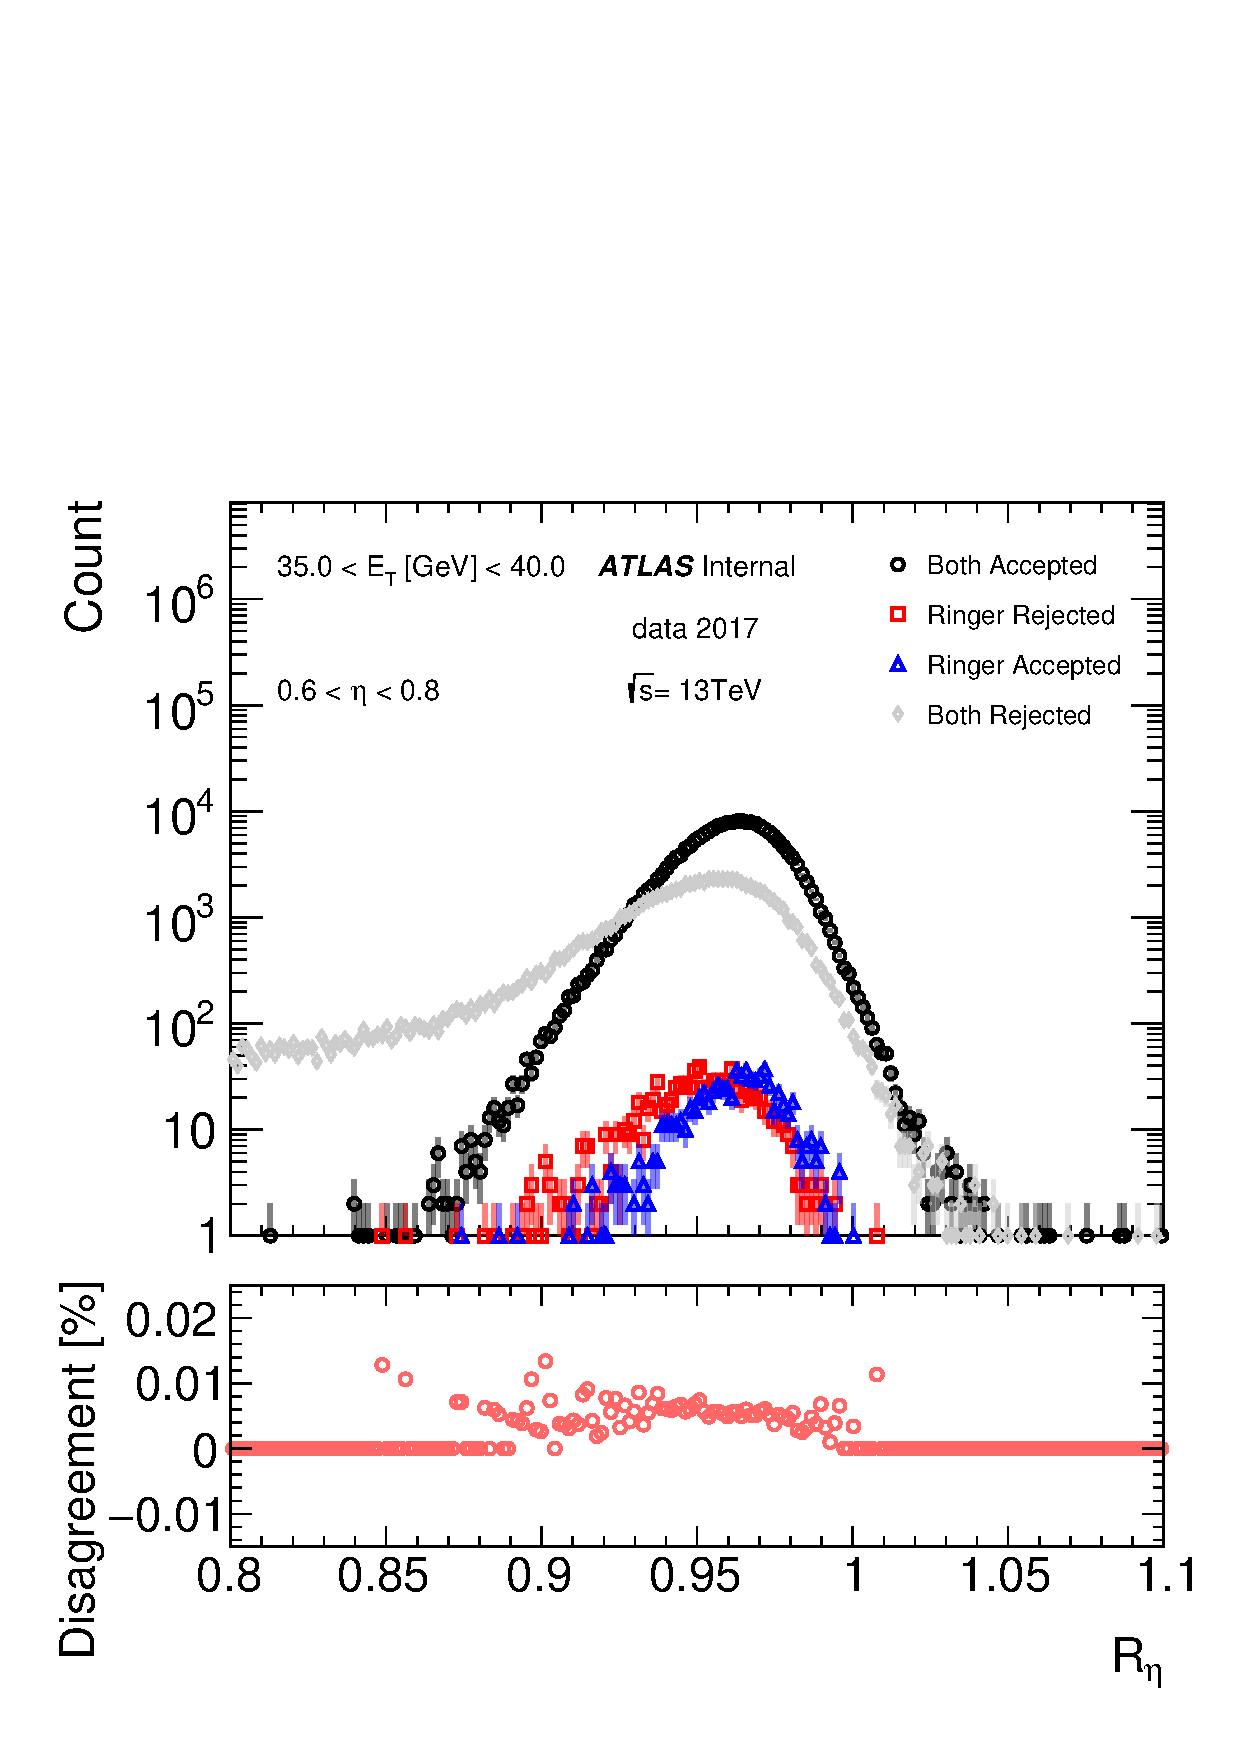
\includegraphics[width=\textwidth]{sections/04_analysis/figures/quadrant_plots/reta.pdf}
\caption{}
\label{fig:quadrant_calo_variables_30GeV_eta}
\end{subfigure}
%\hfill
\begin{subfigure}[c]{.49\textwidth}
\centering
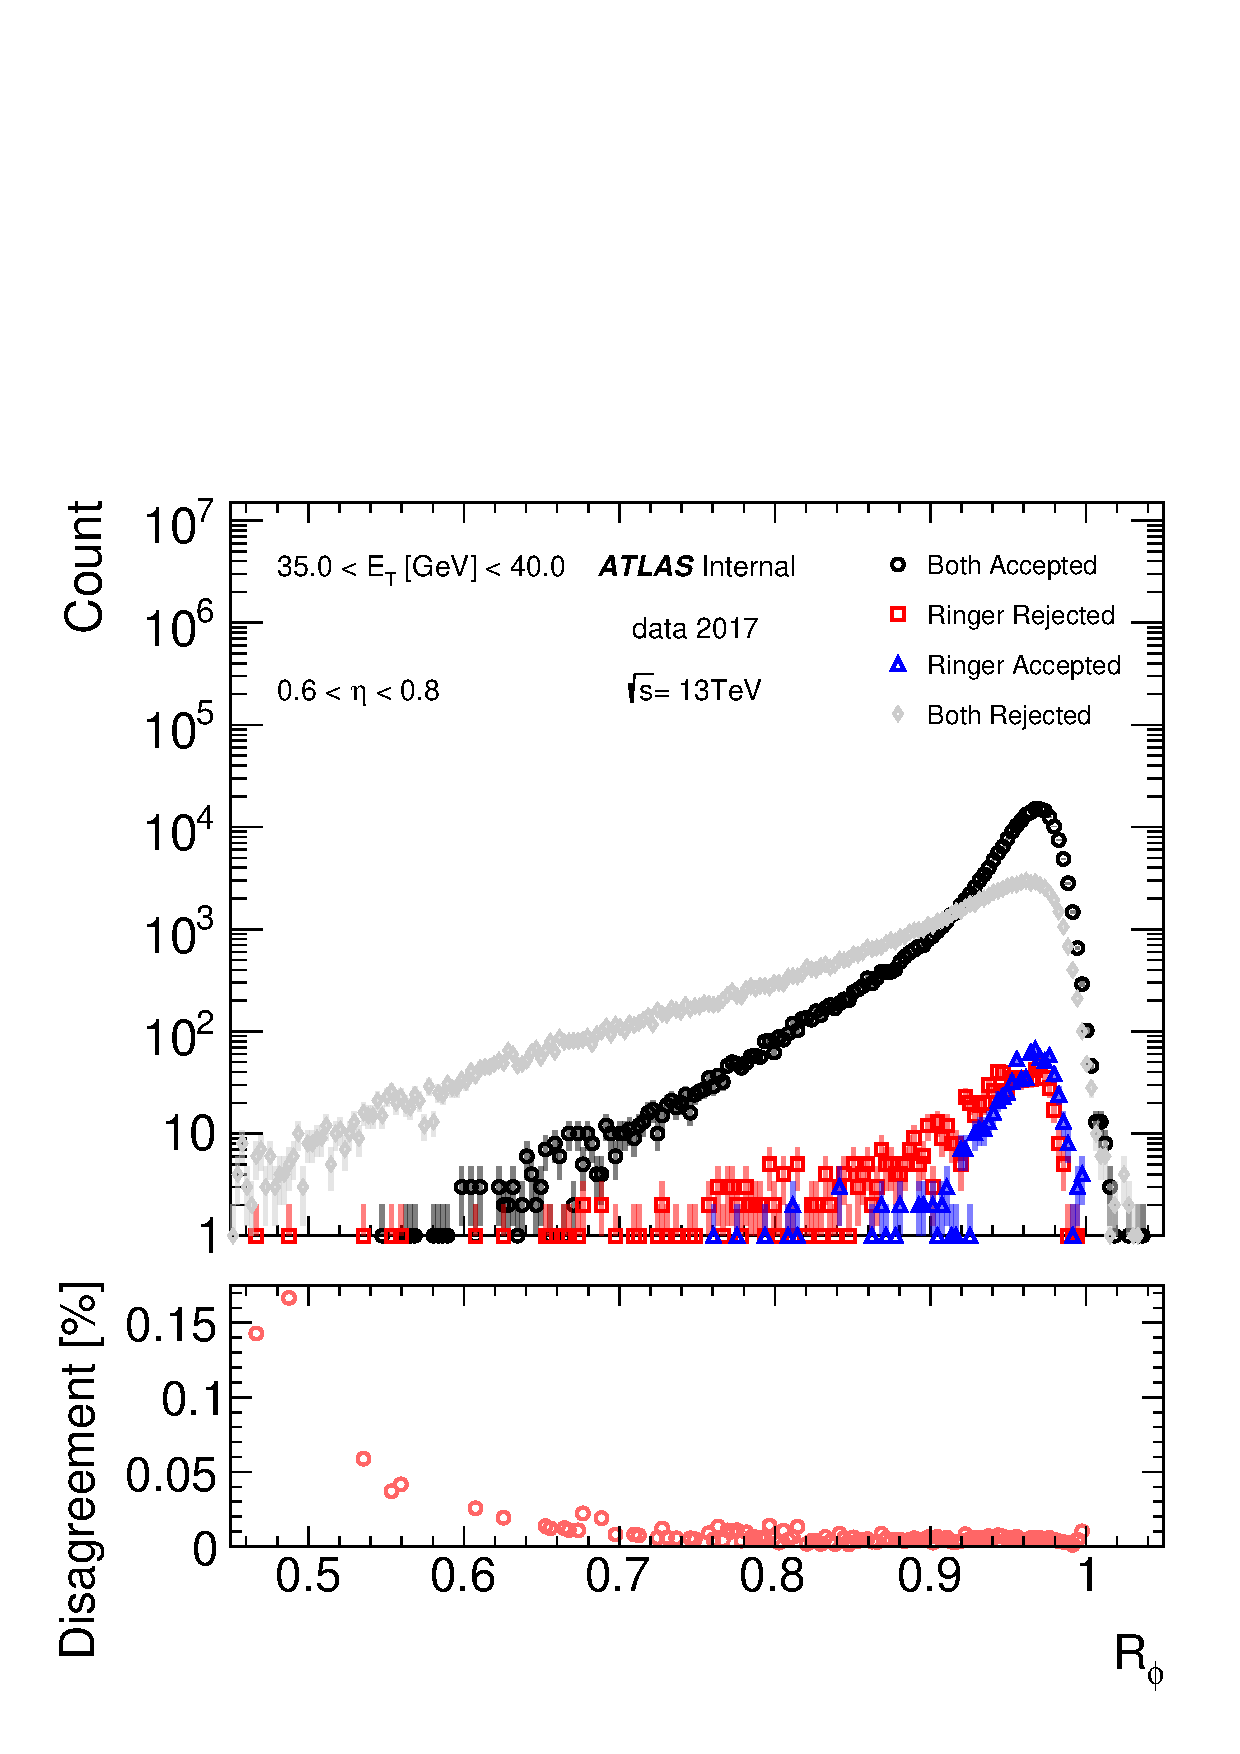
\includegraphics[width=\textwidth]{sections/04_analysis/figures/quadrant_plots/rphi.pdf}
\caption{}
\end{subfigure} 
%\end{figure}
%\begin{figure}[p]\ContinuedFloat
\begin{subfigure}[c]{.49\textwidth}
\centering
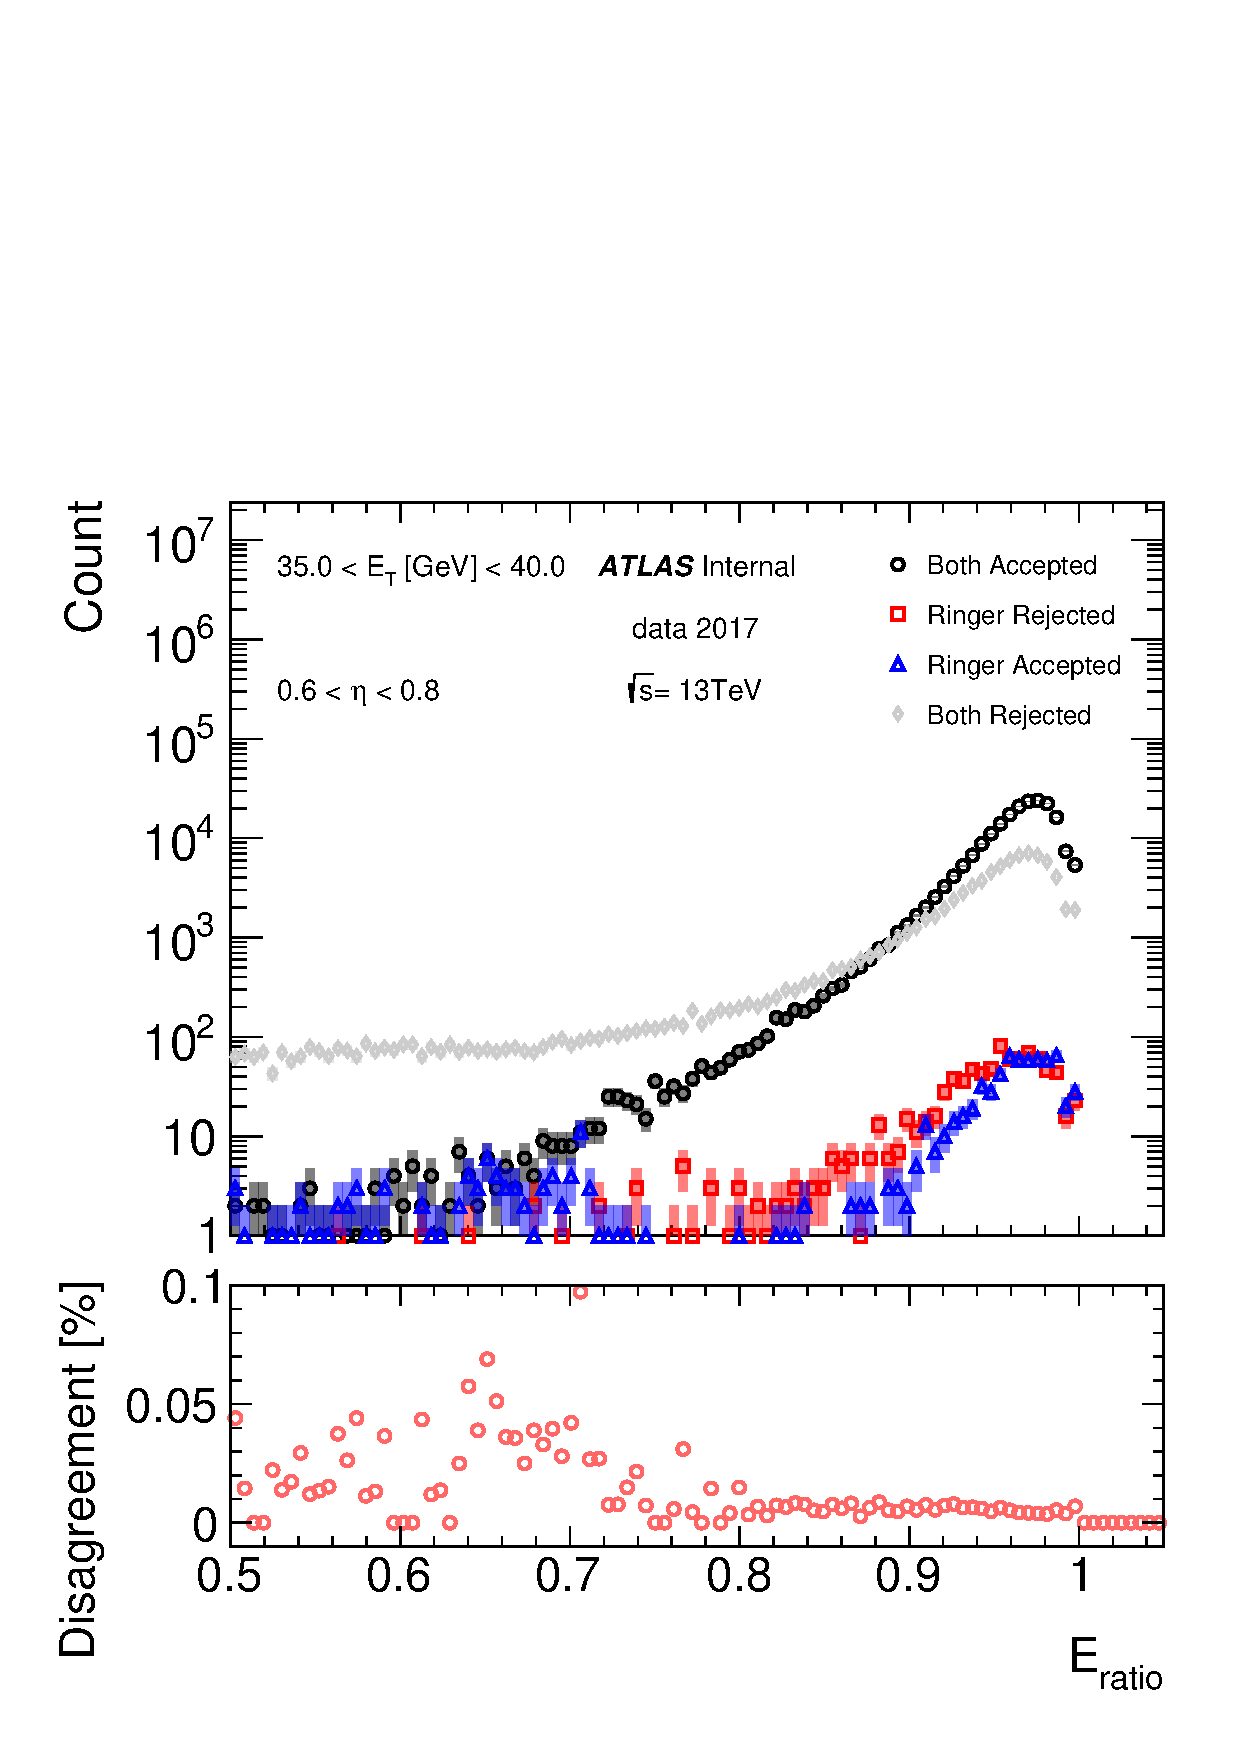
\includegraphics[width=\textwidth]{sections/04_analysis/figures/quadrant_plots/eratio.pdf}
\caption{}
\end{subfigure}
\hfill
\begin{subfigure}[c]{.49\textwidth}
\centering
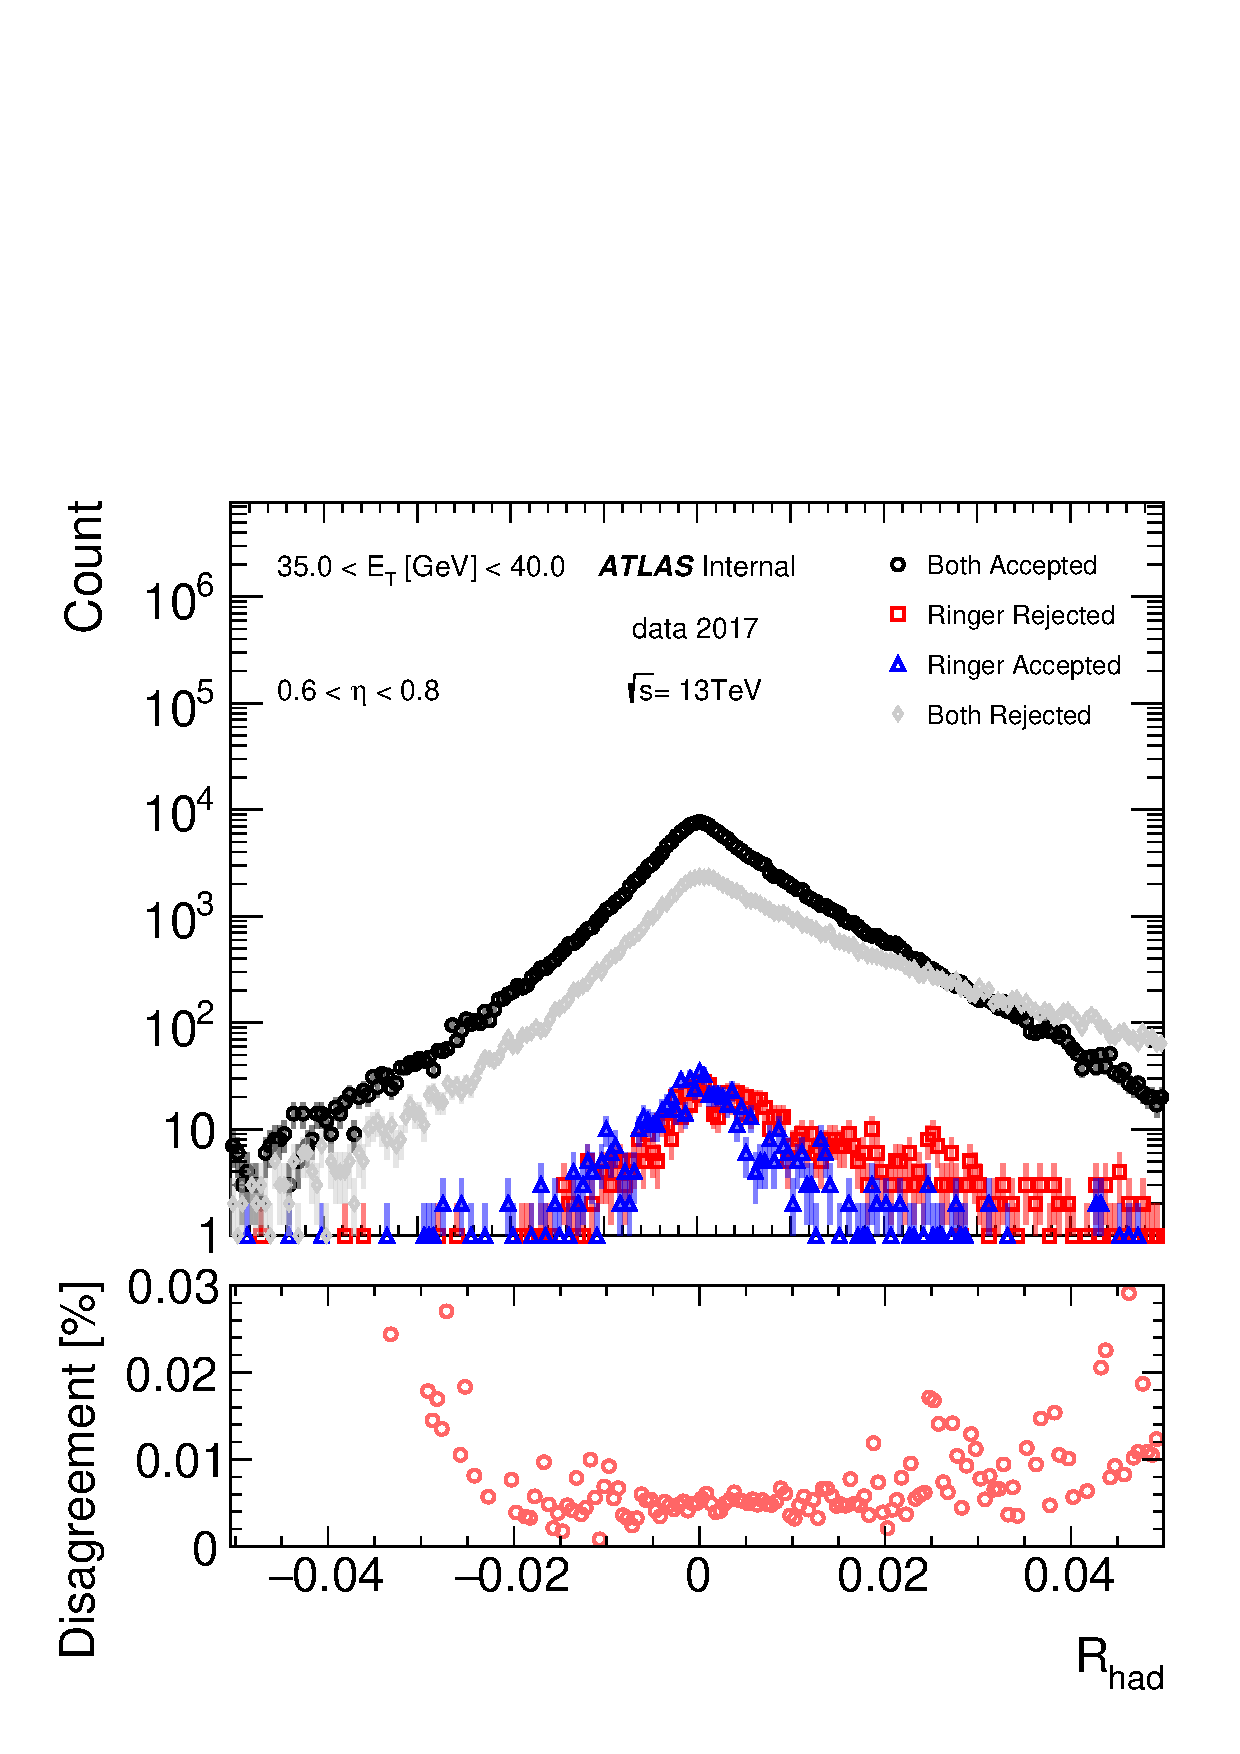
\includegraphics[width=\textwidth]{sections/04_analysis/figures/quadrant_plots/rhad.pdf}
\caption{}
\end{subfigure} \\


\caption{\label{fig:quadrant_calo_variables_30GeV}
	Quadrant analysis plots for the main offline-reconstructed
	calorimetry variables employed in the
	likelihood and for the $0.6<\abseta{}<0.8$ and
	$30<\et{}~[\text{GeV}]<35$ slices. 
	The top pad in each figure shows the raw number of observations for the four mutually exclusive cases: both with and without \rnn{}
	triggered (black); triggered only with \rnn{} (blue); triggered only without \rnn{} (red); neither one triggered (gray). The bottom pad contains disagreement as defined in the Equation \eqref{eq:disagreement}.
}
%Quadrant analysis plots for the offline-reconstructed
%calorimetry variables employed in the
%likelihood and \wstot{} for the $0.6<\abseta{}<0.8$ and
%$30<\et{}~[\text{GeV}]<40$ slices.}%
\end{figure}

Although similar behavior is shown for the other 
regions, the differences vary in strength in each \abseta{} region. As expected, 
the trigger does not show a dependence on ID variables, as shown in Figure~\ref{fig:quadrant_track_variables_30GeV} for $35<\et{}~[\text{GeV}]<40$, since the only distinction between them is the electron identification model operating in the \fastcalo{}.


\begin{comment}
    
\begin{figure}[h!tb]
%\centering
%\begin{subfigure}[c]{.49\textwidth}
\centering
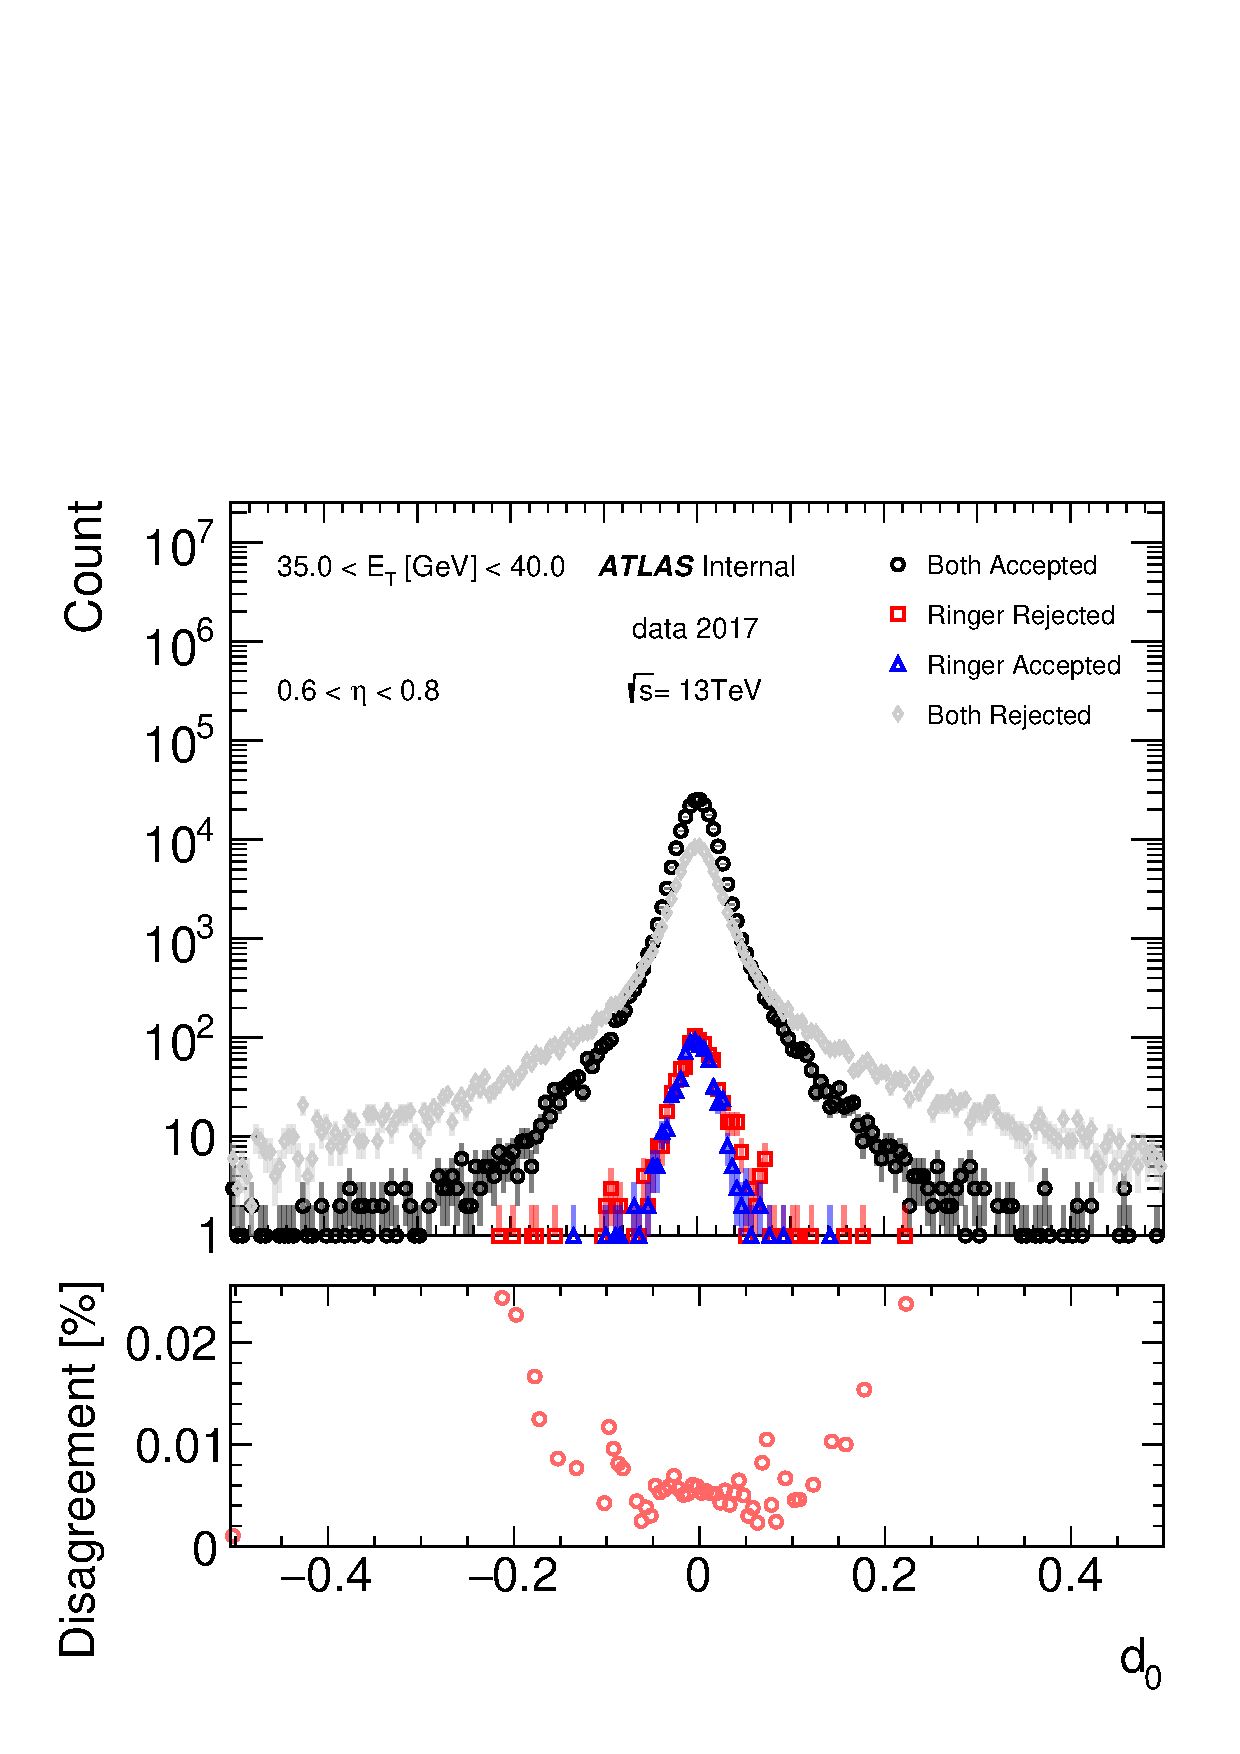
\includegraphics[width=.5\textwidth]{sections/04_analysis/figures/quadrant_plots/d0.pdf}
\caption{\label{fig:quadrant_track_variables_30GeV}
Quadrant analyses plots for the offline-reconstructed ID variable $d_0$ employed in the
likelihood for the $0.6<\abseta{}<0.8$ and $35<\et{}~[\text{GeV}]<40$ slice. The variable $d_0$ is defined as the transverse parameter of the impact point with respect to the collision beam.
}
\end{figure}
\end{comment}






\FloatBarrier
\subsection[Homogeneity Tests]{Homogeneity Tests}\label{ssec:agreement}

In this 
analysis, the impact of using different triggers, \rnn{} and cut-based, on the likelihood algorithm is evaluated. This study requires a pair of duplicated triggers, composed by an $E_T > 28$ GeV isolated and Tight selection with and without the \rnn{}, operating online together. 
This analysis is performed using \Zee{} \tnp{} collision data, which were selected with the trigger requirement set to either one of the duplicated triggers for the tag, whereas the probe selection is invariably set to the offline \vloose{} criterion. This is the exact setup employed by ATLAS to derive the offline likelihood for electrons above \SI{15}{\GeV}~\cite{aaboud2019electron}. To benefit from the full 2017 statistics, collision data collected previous to the TS1 were also employed. In case the profiles are statistically identical, then it is expected that the \rnn{} trigger does not cause any relevant alteration in the derivation of the offline likelihood pdfs.  The statistical method for profile evaluation is described in Section~\ref{top:homogeneity_method} and the results are available in Section~\ref{top:agreement_homogeneity_results}.




\subsubsection{Method}\label{top:homogeneity_method}



The problem is approached based on homogeneity tests on histograms~\cite{homogeneity_test}, in order to check for (systematic) effects of the trigger configuration. It is based on a test originally developed by Pearson~\cite{pearson1911probability} and popularly employed in many fields beyond High Energy Physics (HEP), e.g. social sciences~\cite{wickens2014multiway} and health~\cite{ma2015homogeneity}, usually labelled as contingency or consistency tests.

In order to benefit from the test without having to customize it to the ATLAS particular analysis setup, the collision data was split into two
statistically independent groups attempting to keep data taking conditions as
similar as possible by successively taking data to each group from small
consecutive periods. 

By comparing the p-values of the two groups, it is possible to evaluate how the different configuration affects the likelihood of the profiles to be drawn from the same distribution. If the p-values\footnote{The p-value here is defined by: $P-value \approx f(x, k) = \frac{1}{2^{k/2}\Gamma(k/2)}x^{k/2 -1}e^{-x/2}$} have negligible fluctuations with respect to the values obtained by the tests comparing the same triggers, then the systematic effect in the profiles is negligible with respect to half\footnote{Once each group is using nearly half of the integrated luminosity.} of the statistics available.



To provide a better insight on possible distortions, the corresponding $\chi$
individual contributions of each group are computed allowing them to freely
oscillate through the positive and negative axis with

\begin{equation}
  \chi_{i,j}^{s} = \frac{(r_{i,j} - b_{i,j})}{\sqrt{b_{i,j}}},
  \label{eq:signed_chi}
\end{equation}

\noindent where $r_{i,j}$ ($b_{i,j}$) is the number of observations collected by
the trigger with (without) \rnn{} in $j$th histogram bin and in the $i$th
$\et{}\times\abseta{}$ region.


\subsubsection{Results}\label{top:agreement_homogeneity_results}




Regardless of the trigger configuration, the p-values of the homogeneity tests between the two groups result in similar values. In other words, the fluctuations in the profiles are mainly dominated by statistical fluctuations, with no sign of systematic effects due to the trigger configuration. 

Similar behavior is observed for the ID and calo-ID variables. The Figure~\ref{fig:groups_homogeneity_calo} shows the residuals when considering the histogram obtained with collision data collected by the trigger without \rnn{} for the first arbitrary group as a reference. The residuals are dominated by statistical fluctuations, which are within the expectations from homogeneity hypothesis for most variables and regions.


\begin{figure}[b]
\begin{center}
\begin{subfigure}[c]{.48\textwidth}
\centering
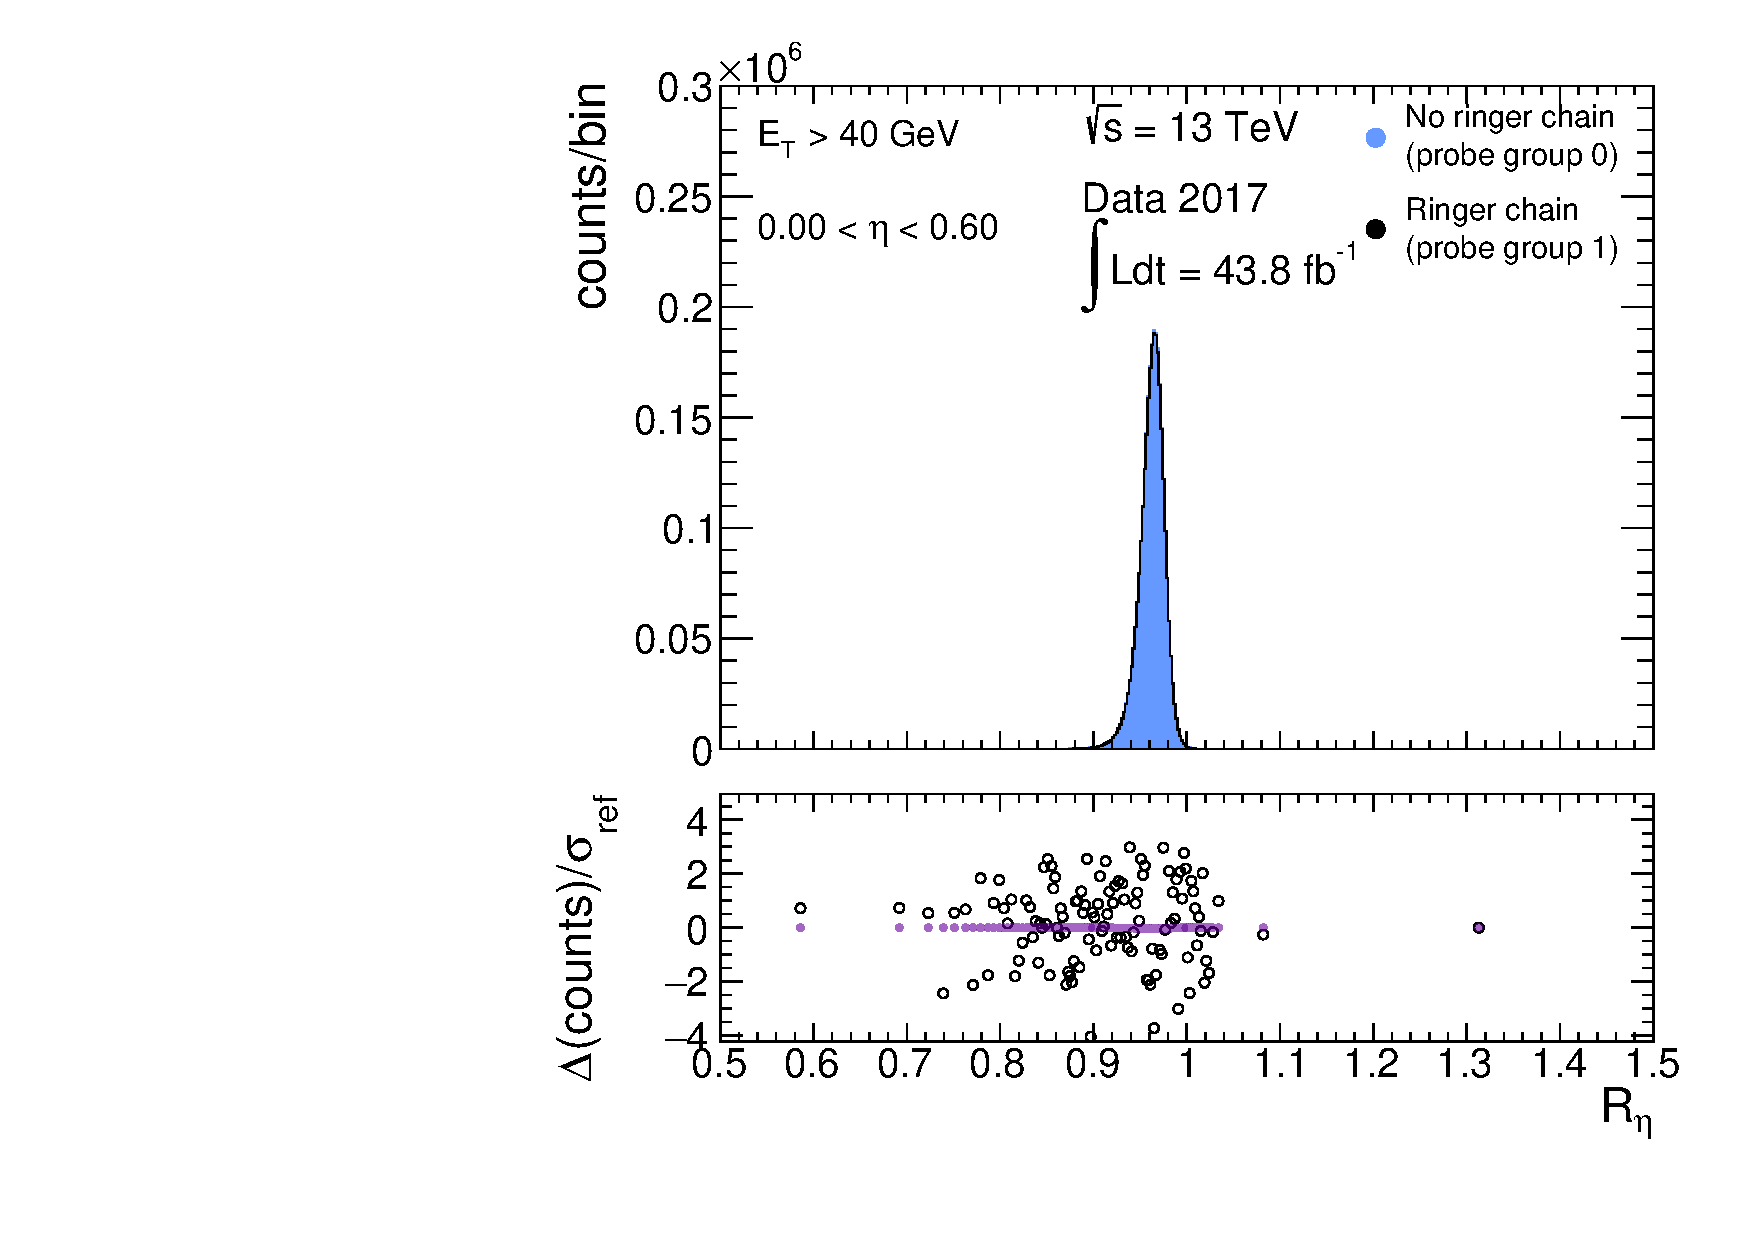
\includegraphics[width=\textwidth]{sections/04_analysis/figures/noAdjustment/el_reta_et40eta0_00_sigma_base_new.pdf}
\caption{}%

\end{subfigure}
\hfill
\begin{subfigure}[c]{.48\textwidth}
\centering
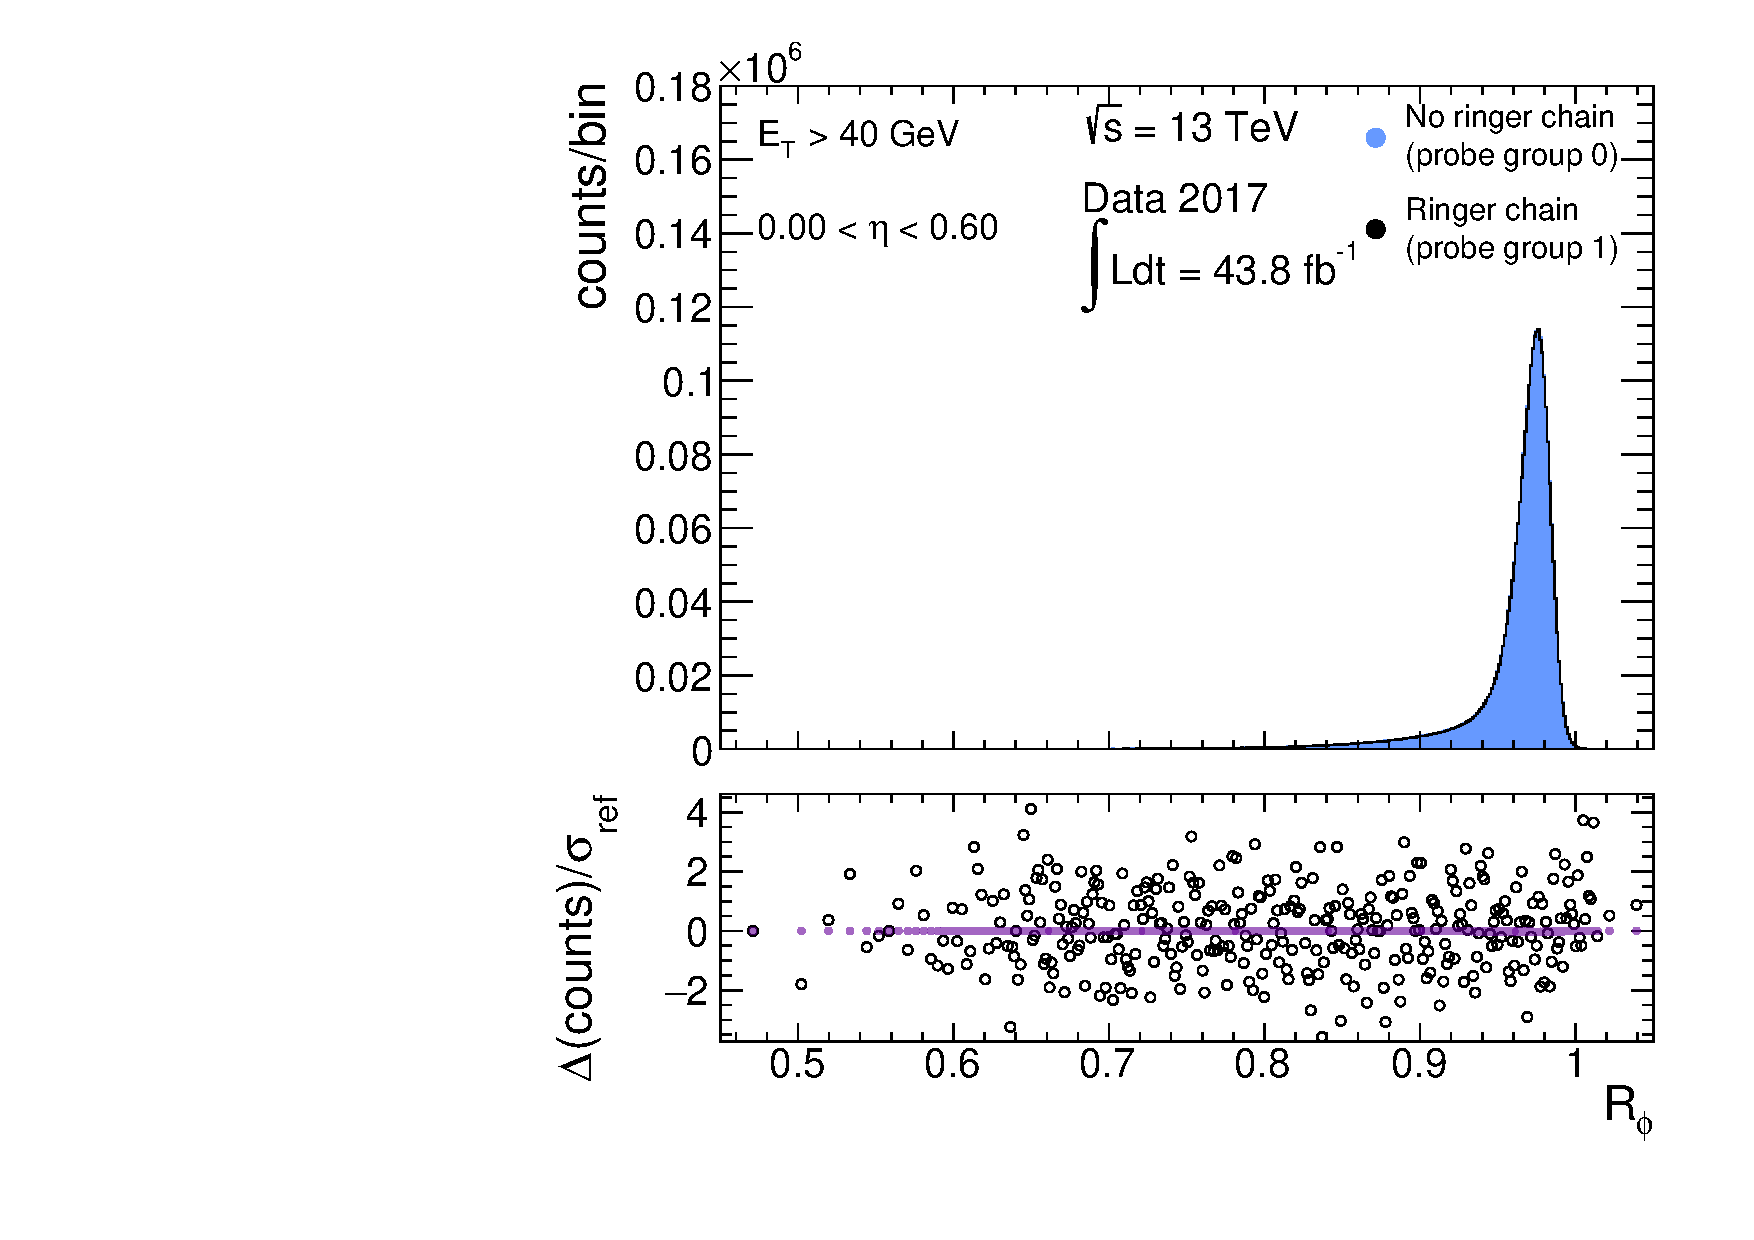
\includegraphics[width=\textwidth]{sections/04_analysis/figures/noAdjustment/el_rphi_et40eta0_00_sigma_base_new.pdf}
\caption{}%

\end{subfigure} \\
\begin{subfigure}[c]{.48\textwidth}
\centering
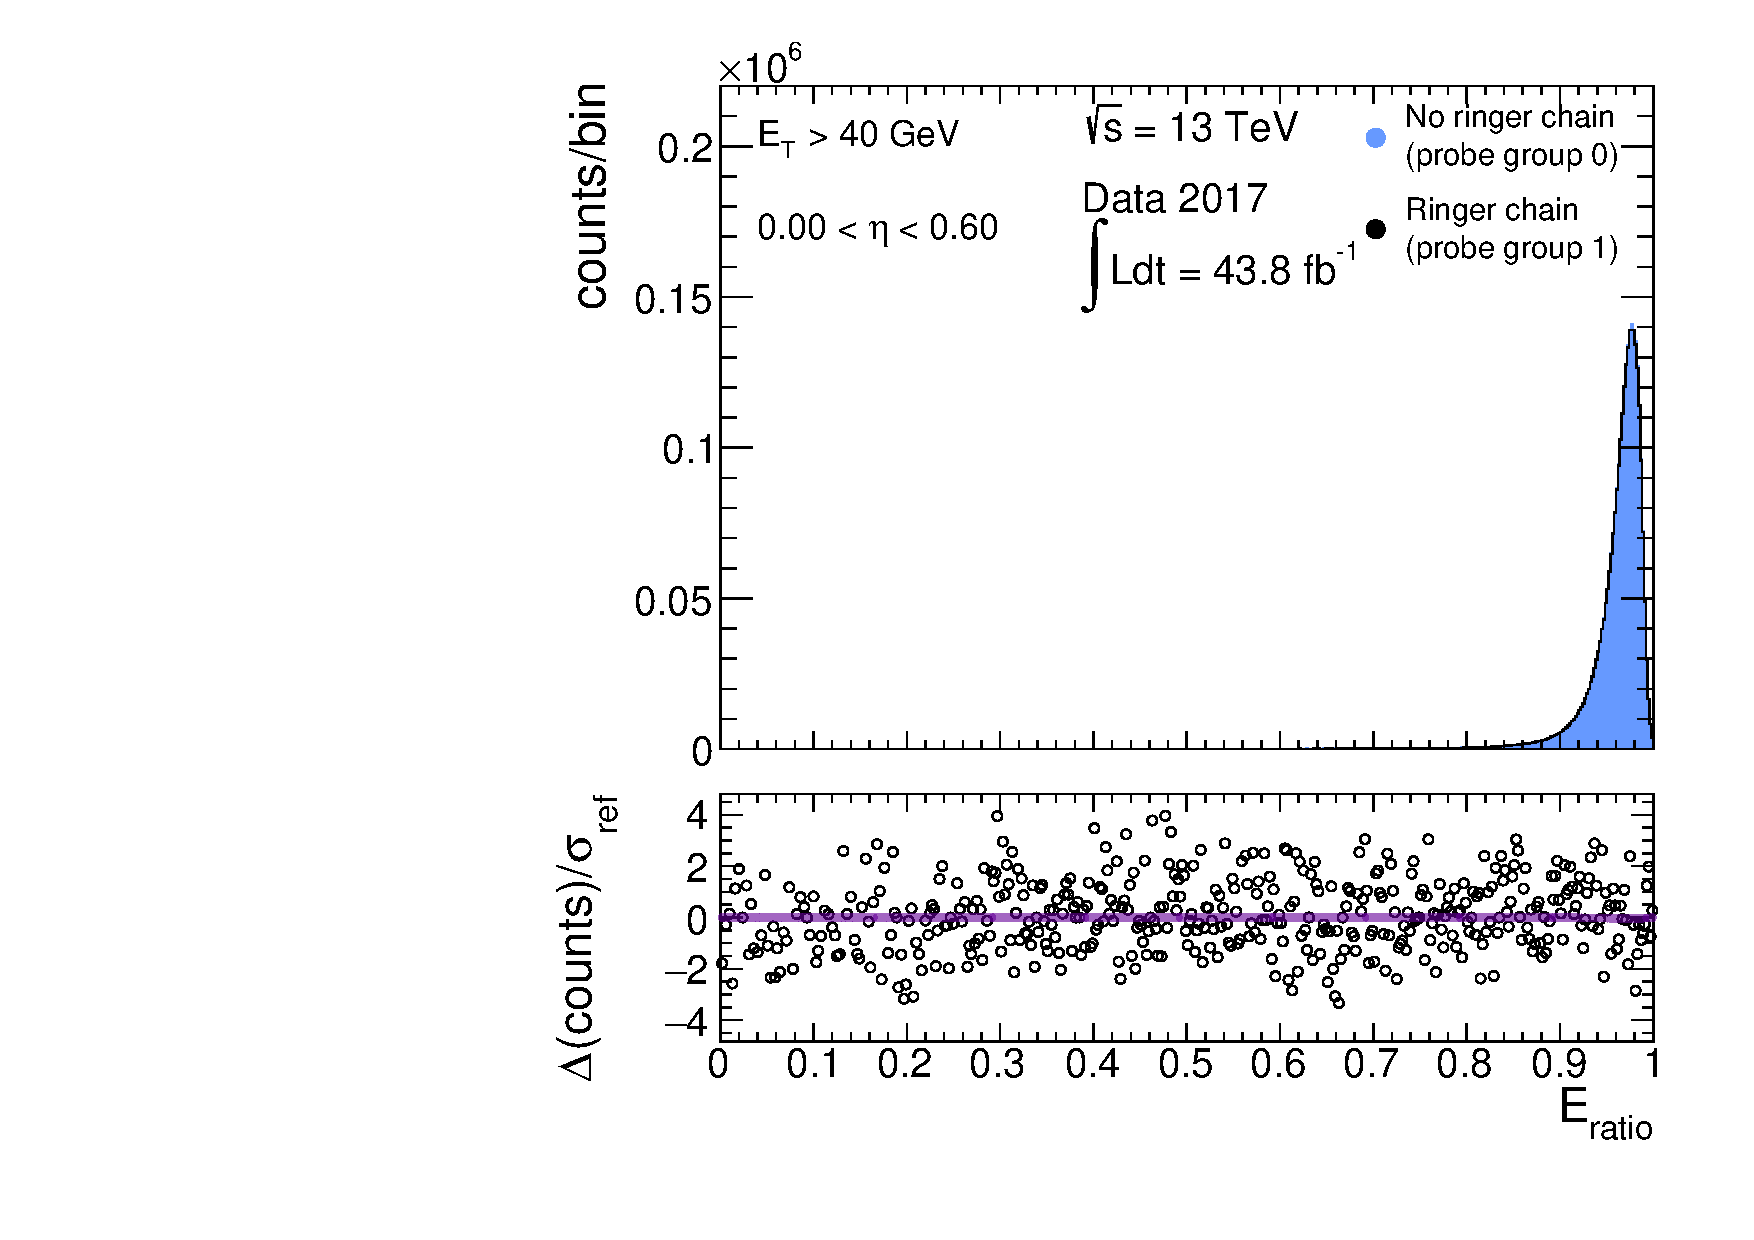
\includegraphics[width=\textwidth]{sections/04_analysis/figures/noAdjustment/el_eratio_et40eta0_00_sigma_base_new.pdf}
\caption{}%

\end{subfigure}
\hfill
\begin{subfigure}[c]{.48\textwidth}
\centering
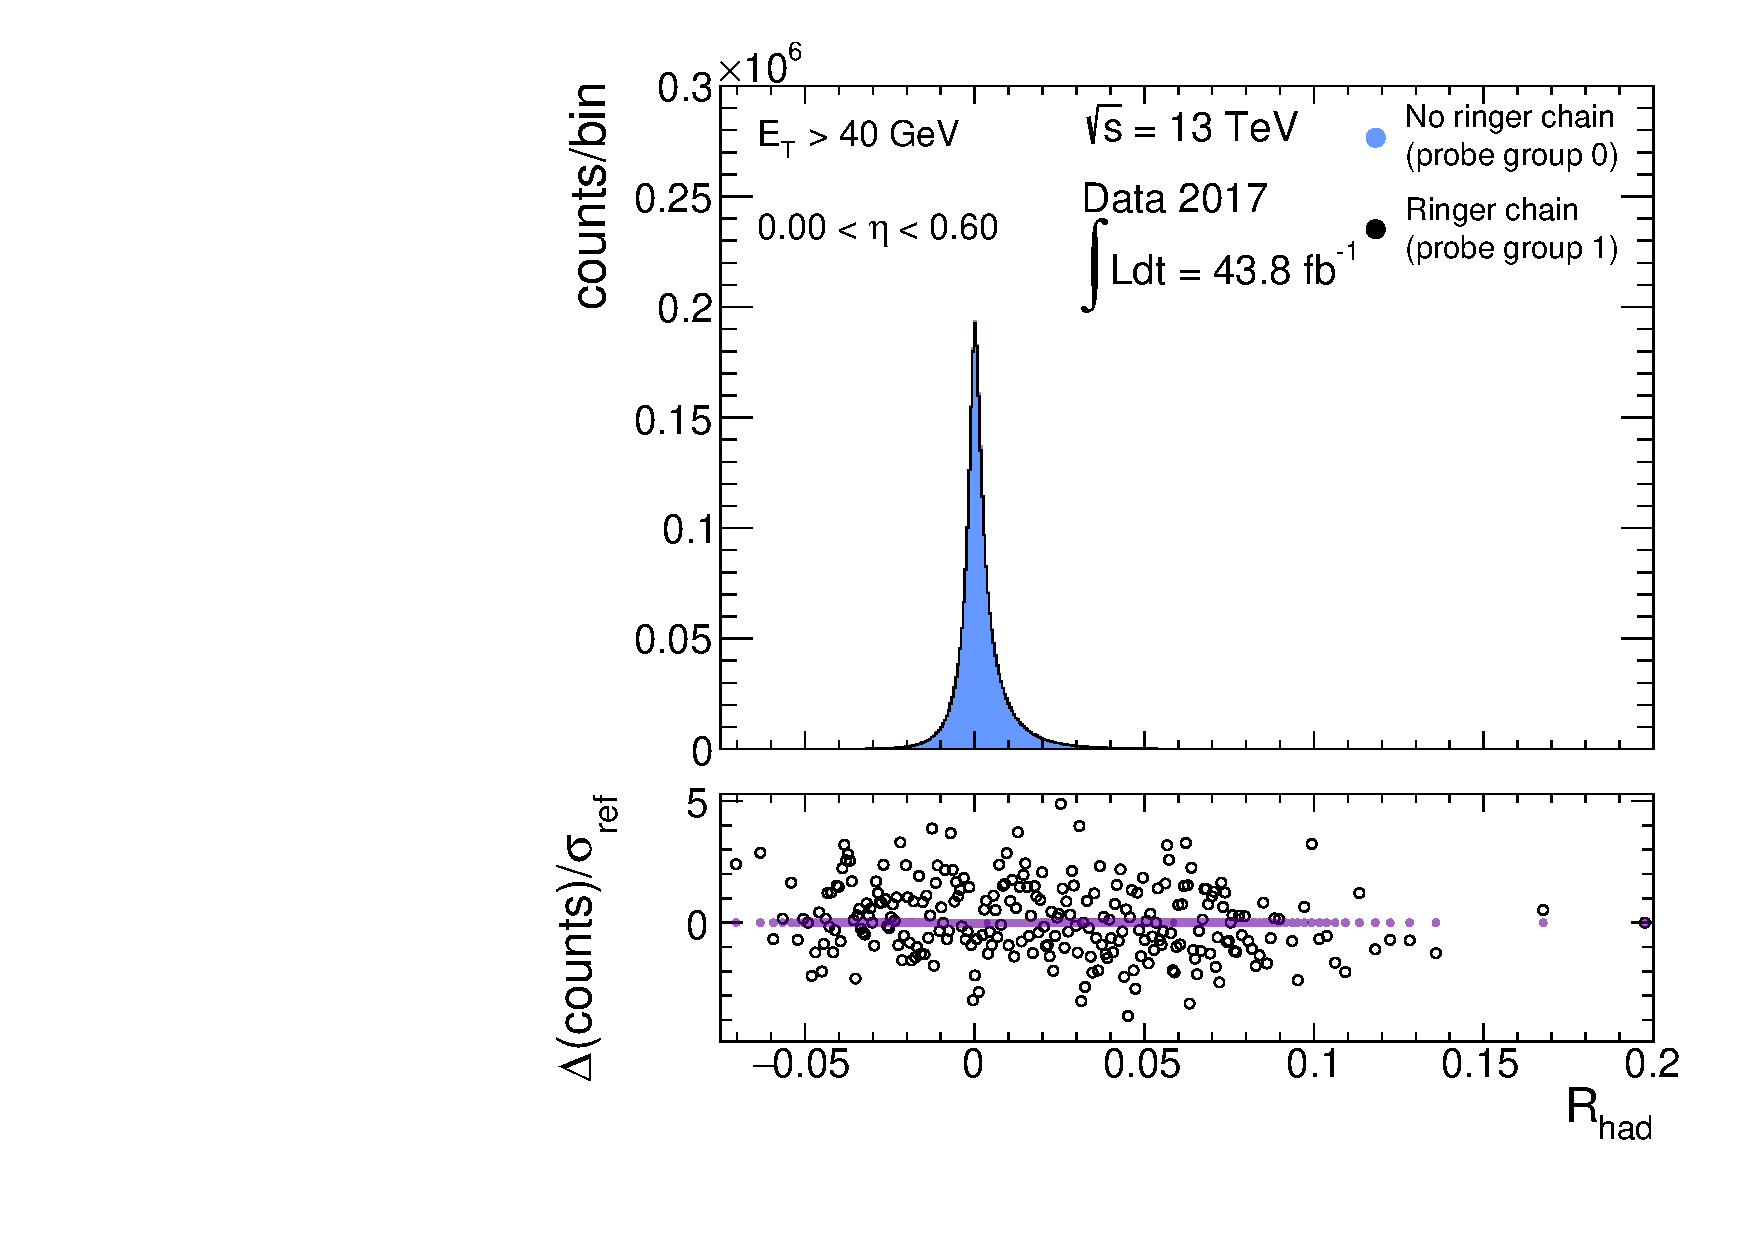
\includegraphics[width=\textwidth]{sections/04_analysis/figures/noAdjustment/el_rhad_et40eta0_00_sigma_base_new.pdf}
\caption{}%

\end{subfigure} \\
\caption{%
	Top: \reta, \eratio, \rphi, \rhad histogram profiles for the calorimetry variables employed in the offline likelihood in the $\et>\SI{40}{\GeV}$ and $0.00<\abseta{}<0.80$ regions using collision data collected by
	triggering without \rnn{} in the first arbitrary data group
	(blue area) and collision data collected by triggering with \rnn{} in the second
	arbitrary data group (black line).  Bottom: residual contributions using as
	statistics $\chi^s$ (equation~\ref{eq:signed_chi}, in black) and the expected
	model for no distortion given by the $\chi^s$ residuals w.r.t.\@ the
	reference.
}%
\label{fig:groups_homogeneity_calo}
\end{center}
\end{figure}%


\FloatBarrier
 % ok
\section{Conclusion}\label{sec:conclusion}
%-------------------------------------------------------------------------------


% Comparison with standard strategies
The \rnn{} is an innovative design for electron selection based on
calorimetry information. With the
ambition to comply with specific trigger system demands, the feature extraction
of concentric ring energy sums provides an efficient description, which is quickly derived through simple operations. Neural network models are employed for exploiting
nonlinear correlations between rings and the optimisation of this strategy culminated in the employment of a set of specialist models per regions of pseudorapidity and transverse energy. 


In the second half of 2017, the \rnn{} algorithm replaced such a cut-based strategy
in the \fastcalo{} decision step and became the baseline algorithm
for triggering events containing electrons above \SI{15}{\GeV}, as part of the ATLAS online system CPU reduction campaign. The \fastcalo{} selection is crucial for CPU demands, as a more
efficient algorithm allows to avoid heavier computations in the
subsequent steps.  It was the first time a neural network method was employed as
a baseline selection algorithm for event selection in the ATLAS trigger system.


During 2017 operation, based on neural networks trained with simulated data, a
reduction factors of 13 in the \fastcalo{} and of 2 in
the \hlt{} of fake rates were achieved with respect to the offline likelihood, while
keeping high electron efficiency when the \rnn{} was set to operate in a
configuration similar to lowest energy-threshold unprescaled single electron
trigger. For 2018, the \rnn{} was trained with collision
data resulting in an estimated additional reduction factor of 1.19--1.69 in the  \fastcalo{} with respect to 2017. 


Additionally, the \rnn{} was also studied through the offline likelihood perspective to bring additional insights on its behavior using two equivalent single electron trigger with and without the \rnn{}.
The proposed quadrant analysis
allowed to observe high agreement between both triggers with slight shifts
towards the signal region in the disagreement profiles of some calorimetry-based
variables. Finally, when considering homogeneity test, the p-values of the between the two groups result in similar values. In other words, the fluctuations in the profiles are mainly dominated by statistical fluctuations, with no sign of systematic effects due to the trigger configuration.




\begin{comment}



    


% Quadrant and agreement analysis
The \rnn{} was also studied through the offline likelihood perspective 
to bring additional insights on its behavior. By
taking advantage of the low dimensionality, low correlation and high
interpretability power of the variables employed in the likelihood, we derived
the profiles of the disjoint decision cases of the 2017 duplicate trigger pair.
The choice for the duplicated pair considered the typical scenario employed for
analysis with the setup that would maximize the disagreement between both
configurations: with and without the \rnn{}. The proposed quadrant analysis
allowed to observe high agreement between both triggers with slight shifts
towards the signal region in the disagreement profiles of some calorimetry-based
variables. By checking the agreement between the trigger pair for the derivation
of the likelihood pdfs, the alteration using the full 2017 data was much lower
than estimated statistical fluctuations. The residuals were found to be bounded
by \SI{0.2}{$\sigma$} for all variables. When considering only the
disagreement profiles, homogeneity hypothesis at a \SI{5}{\%} level was not
rejected for the calorimetry variables, except for \reta{} and \rhad{} despite
using the most populated regions. For these variables, a shift towards signal
region was also observed. Hence, the \rnn{} had negligible impact in the
sensitive variables employed for physics analysis and in the offline selection
operation.

Finally, the presented results show that it is possible to tighten the requirements for online operation while still resulting in high agreement with the offline
selection. More generally, it demonstrates that designing a solution from scratch using the application specificities can provide new effective
strategies. We hope that it can serve as motivation for other developments in
HEP, particularly when considering the trigger applications.

\section{Outlook}


Preliminary evaluations have shown the potential of the \rnn{} algorithm for
triggering on electrons with $\et<\SI{15}{\GeV}$. This is particularly motivating given that triggers in this kinematic region are very
CPU demanding. Additionally, they have high output rate and are usually
prescaled, thus \rnn{} might also allow to collect additional data for those
triggers. For the beginning of Run 3 (2022), \rnn{} has been extended to all triggers below $\et<\SI{15}{\GeV}$ where a reduction of at least half of the fake rate in \fastcalo was observed.


Photons are other physics objects that may be triggered using the Ringer approach. Triggers combining photons to other physics objects are quite CPU demanding, thus motivating studies to evaluate whether additional Ringer developments will contribute to increased performance.
When considering pure photon triggers, the ring sums with linear classifiers can be investigated in order to keep the analysis strategies employed in channels as $\text{H}\rightarrow Z\gamma$. Another possibility for those triggers is to
employ the \rnn{} for increasing the trigger efficiency. A possible
setup is to duplicate the photon triggers so that the \rnn{} recovers
interesting events.  In this hybrid menu configuration, the standard trigger
would be available for those analyses so that they may benefit from high
interpretability and customization, whereas the \rnn{} trigger might be employed
for those analyses demanding more statistics. It is expected that this
configuration will demand minor additional resources but may allow higher
statistical significance of the results of physics analysis.


% No-had
Another interesting possibility is to employ the \rnn{} accessing only
electromagnetic information for triggers resulting in high readout rate from
hadronic calorimeter cells. The particular setup may even consider employing a
two step decision on the \fastcalo{}, a preliminary one based solely on
electromagnetic information followed by the full \rnn{} decision.




% Boosted configurations
Physics beyond the Standard Model is getting more attention at the LHC and is expected to be part of the main focus in the data-taking phases to
come. We aim at improving the \rnn{} algorithm to comprise boosted
configurations, particularly limiting the effect of other contributions at
the edge of the feature extraction window, which can result from these physics
processes. Additionally, the \rnn{} is being evaluated as an alternative
strategy for a long-lived particle analysis. %($\text{a}\rightarrow\text{H}(\gamma\gamma)Z(l^+l^-)$).


Nevertheless, we expect that the \rnn{} efficiency can still be improved. Indeed, the feature extraction
algorithm has many limitations as being initially proposed for online
operation, but a more complex algorithm accounting for the cell sizes can
provide more precise information, which, eventually, can be helpful for the
selection task. Shower asymmetries may be captured if extracting ring segments,
i.e.\@ quarter rings delimited by $\eta\times\phi$ axis. Complementary
discriminant information may be obtained by fusing the ring sums with the shower shape variables,
which is under investigation. Deep learning models can be exploited instead of
single hidden-layer MLPs, in order to achieve better suited decision boundaries,
specially considering models designed to exploit the sequential structure
presented by the rings.


% Calibration
The shower description by ring sums goes beyond capturing discriminant
information and may be used for calibration of the energy of electrons and
photons. While preliminary results with ring sums are motivating, we expect the aforementioned
improvements in the ring description to be exceptionally important for
calibration.

% Offline developments
The \rnn{} software has been extended to the offline framework. Currently,
the offline ring description is available for all electrons with $\et>\SI{14}{\GeV}$. This is an on-going activity.


\end{comment}
 % ok

%-------------------------------------------------------------------------------
% When your ATLAS paper or PUB/CONF note is ready to be published,
% the acknowledgements should be automatically included/updated by PO-GitLab.
% The acknowledgements can be inspected on the web page:
% \url{https://atlas-glance.cern.ch/atlas/membership/funding_agencies/history}.
\section*{Acknowledgements}
%-------------------------------------------------------------------------------

% Acknowledgements - comment in this line when you are ready to include them.
% Acknowledgements for papers with collision data
% Version 2024-07-11
 
% Standard acknowledgements start here
%----------------------------------------------
 
We thank CERN for the very successful operation of the LHC and its injectors, as well as the support staff at
CERN and at our institutions worldwide without whom ATLAS could not be operated efficiently.
 
The crucial computing support from all WLCG partners is acknowledged gratefully, in particular from CERN, the ATLAS Tier-1 facilities at TRIUMF/SFU (Canada), NDGF (Denmark, Norway, Sweden), CC-IN2P3 (France), KIT/GridKA (Germany), INFN-CNAF (Italy), NL-T1 (Netherlands), PIC (Spain), RAL (UK) and BNL (USA), the Tier-2 facilities worldwide and large non-WLCG resource providers. Major contributors of computing resources are listed in Ref.~\cite{ATL-SOFT-PUB-2023-001}.
 
We gratefully acknowledge the support of ANPCyT, Argentina; YerPhI, Armenia; ARC, Australia; BMWFW and FWF, Austria; ANAS, Azerbaijan; CNPq and FAPESP, Brazil; NSERC, NRC and CFI, Canada; CERN; ANID, Chile; CAS, MOST and NSFC, China; Minciencias, Colombia; MEYS CR, Czech Republic; DNRF and DNSRC, Denmark; IN2P3-CNRS and CEA-DRF/IRFU, France; SRNSFG, Georgia; BMBF, HGF and MPG, Germany; GSRI, Greece; RGC and Hong Kong SAR, China; ISF and Benoziyo Center, Israel; INFN, Italy; MEXT and JSPS, Japan; CNRST, Morocco; NWO, Netherlands; RCN, Norway; MNiSW, Poland; FCT, Portugal; MNE/IFA, Romania; MESTD, Serbia; MSSR, Slovakia; ARRS and MIZ\v{S}, Slovenia; DSI/NRF, South Africa; MICINN, Spain; SRC and Wallenberg Foundation, Sweden; SERI, SNSF and Cantons of Bern and Geneva, Switzerland; MOST, Taipei; TENMAK, T\"urkiye; STFC, United Kingdom; DOE and NSF, United States of America.
 
Individual groups and members have received support from BCKDF, CANARIE, CRC and DRAC, Canada; CERN-CZ, FORTE and PRIMUS, Czech Republic; COST, ERC, ERDF, Horizon 2020, ICSC-NextGenerationEU and Marie Sk{\l}odowska-Curie Actions, European Union; Investissements d'Avenir Labex, Investissements d'Avenir Idex and ANR, France; DFG and AvH Foundation, Germany; Herakleitos, Thales and Aristeia programmes co-financed by EU-ESF and the Greek NSRF, Greece; BSF-NSF and MINERVA, Israel; NCN and NAWA, Poland; La Caixa Banking Foundation, CERCA Programme Generalitat de Catalunya and PROMETEO and GenT Programmes Generalitat Valenciana, Spain; G\"{o}ran Gustafssons Stiftelse, Sweden; The Royal Society and Leverhulme Trust, United Kingdom.
 
In addition, individual members wish to acknowledge support from Armenia: Yerevan Physics Institute (FAPERJ); CERN: European Organization for Nuclear Research (CERN PJAS); Chile: Agencia Nacional de Investigaci\'on y Desarrollo (FONDECYT 1230812, FONDECYT 1230987, FONDECYT 1240864); China: Chinese Ministry of Science and Technology (MOST-2023YFA1605700), National Natural Science Foundation of China (NSFC - 12175119, NSFC 12275265, NSFC-12075060); Czech Republic: Czech Science Foundation (GACR - 24-11373S), Ministry of Education Youth and Sports (FORTE CZ.02.01.01/00/22\_008/0004632), PRIMUS Research Programme (PRIMUS/21/SCI/017); EU: H2020 European Research Council (ERC - 101002463); European Union: European Research Council (ERC - 948254, ERC 101089007), Horizon 2020 Framework Programme (MUCCA - CHIST-ERA-19-XAI-00), European Union, Future Artificial Intelligence Research (FAIR-NextGenerationEU PE00000013), Italian Center for High Performance Computing, Big Data and Quantum Computing (ICSC, NextGenerationEU); France: Agence Nationale de la Recherche (ANR-20-CE31-0013, ANR-21-CE31-0013, ANR-21-CE31-0022), Investissements d'Avenir Labex (ANR-11-LABX-0012); Germany: Baden-Württemberg Stiftung (BW Stiftung-Postdoc Eliteprogramme), Deutsche Forschungsgemeinschaft (DFG - 469666862, DFG - CR 312/5-2); Italy: Istituto Nazionale di Fisica Nucleare (ICSC, NextGenerationEU); Japan: Japan Society for the Promotion of Science (JSPS KAKENHI JP22H01227, JSPS KAKENHI JP22H04944, JSPS KAKENHI JP22KK0227, JSPS KAKENHI JP23KK0245); Netherlands: Netherlands Organisation for Scientific Research (NWO Veni 2020 - VI.Veni.202.179); Norway: Research Council of Norway (RCN-314472); Poland: Ministry of Science and Higher Education (IDUB AGH, POB8, D4 no 9722), Polish National Agency for Academic Exchange (PPN/PPO/2020/1/00002/U/00001), Polish National Science Centre (NCN 2021/42/E/ST2/00350, NCN OPUS nr 2022/47/B/ST2/03059, NCN UMO-2019/34/E/ST2/00393, UMO-2020/37/B/ST2/01043, UMO-2021/40/C/ST2/00187, UMO-2022/47/O/ST2/00148, UMO-2023/49/B/ST2/04085, UMO-2023/51/B/ST2/00920); Slovenia: Slovenian Research Agency (ARIS grant J1-3010); Spain: Generalitat Valenciana (Artemisa, FEDER, IDIFEDER/2018/048), Ministry of Science and Innovation (MCIN \& NextGenEU PCI2022-135018-2, MICIN \& FEDER PID2021-125273NB, RYC2019-028510-I, RYC2020-030254-I, RYC2021-031273-I, RYC2022-038164-I); Sweden: Swedish Research Council (Swedish Research Council 2023-04654, VR 2018-00482, VR 2022-03845, VR 2022-04683, VR 2023-03403, VR grant 2021-03651), Knut and Alice Wallenberg Foundation (KAW 2018.0458, KAW 2019.0447, KAW 2022.0358); Switzerland: Swiss National Science Foundation (SNSF - PCEFP2\_194658); United Kingdom: Leverhulme Trust (Leverhulme Trust RPG-2020-004), Royal Society (NIF-R1-231091); United States of America: U.S. Department of Energy (ECA DE-AC02-76SF00515), Neubauer Family Foundation.
 
%----------------------------------------------
% Created with Glance


%-------------------------------------------------------------------------------
\clearpage
%\appendix
%\part*{Appendix}
%\addcontentsline{toc}{part}{Appendix}
%-------------------------------------------------------------------------------
%In a paper, an appendix is used for technical details that would otherwise disturb the flow of the paper.
%Such an appendix should be printed before the Bibliography.

%-------------------------------------------------------------------------------
% If you use biblatex and either biber or bibtex to process the bibliography
% just say \printbibliography here.
\printbibliography
% If you want to use the traditional BibTeX you need to use the syntax below.
% \bibliographystyle{obsolete/bst/atlasBibStyleWoTitle}
% \bibliography{ANA-TRIG-2021-01-PAPER,bib/ATLAS,bib/CMS,bib/ConfNotes,bib/PubNotes}
%-------------------------------------------------------------------------------

%-------------------------------------------------------------------------------
% Author list - comment in these two lines when you are ready to include them.
% \clearpage
% % ATLAS Collaboration author list
% Reference date of TRIG-2021-01 is 2024-07-11
% Data extracted on 11-Jul-2024 for paper reference TRIG-2021-01
% at 7:19pm
 
\begin{flushleft}
\hypersetup{urlcolor=black}
{\Large The ATLAS Collaboration}

\bigskip

\AtlasOrcid[0000-0002-6665-4934]{G.~Aad}$^\textrm{\scriptsize 105}$,
\AtlasOrcid[0000-0001-7616-1554]{E.~Aakvaag}$^\textrm{\scriptsize 17}$,
\AtlasOrcid[0000-0002-5888-2734]{B.~Abbott}$^\textrm{\scriptsize 124}$,
\AtlasOrcid[0000-0002-0287-5869]{S.~Abdelhameed}$^\textrm{\scriptsize 120a}$,
\AtlasOrcid[0000-0002-1002-1652]{K.~Abeling}$^\textrm{\scriptsize 57}$,
\AtlasOrcid[0000-0001-5763-2760]{N.J.~Abicht}$^\textrm{\scriptsize 51}$,
\AtlasOrcid[0000-0002-8496-9294]{S.H.~Abidi}$^\textrm{\scriptsize 30}$,
\AtlasOrcid[0009-0003-6578-220X]{M.~Aboelela}$^\textrm{\scriptsize 46}$,
\AtlasOrcid[0000-0002-9987-2292]{A.~Aboulhorma}$^\textrm{\scriptsize 36e}$,
\AtlasOrcid[0000-0001-5329-6640]{H.~Abramowicz}$^\textrm{\scriptsize 155}$,
\AtlasOrcid[0000-0002-1599-2896]{H.~Abreu}$^\textrm{\scriptsize 154}$,
\AtlasOrcid[0000-0003-0403-3697]{Y.~Abulaiti}$^\textrm{\scriptsize 121}$,
\AtlasOrcid[0000-0002-8588-9157]{B.S.~Acharya}$^\textrm{\scriptsize 71a,71b,k}$,
\AtlasOrcid[0000-0003-4699-7275]{A.~Ackermann}$^\textrm{\scriptsize 65a}$,
\AtlasOrcid[0000-0002-2634-4958]{C.~Adam~Bourdarios}$^\textrm{\scriptsize 4}$,
\AtlasOrcid[0000-0002-5859-2075]{L.~Adamczyk}$^\textrm{\scriptsize 88a}$,
\AtlasOrcid[0000-0002-2919-6663]{S.V.~Addepalli}$^\textrm{\scriptsize 27}$,
\AtlasOrcid[0000-0002-8387-3661]{M.J.~Addison}$^\textrm{\scriptsize 104}$,
\AtlasOrcid[0000-0002-1041-3496]{J.~Adelman}$^\textrm{\scriptsize 119}$,
\AtlasOrcid[0000-0001-6644-0517]{A.~Adiguzel}$^\textrm{\scriptsize 22c}$,
\AtlasOrcid[0000-0003-0627-5059]{T.~Adye}$^\textrm{\scriptsize 138}$,
\AtlasOrcid[0000-0002-9058-7217]{A.A.~Affolder}$^\textrm{\scriptsize 140}$,
\AtlasOrcid[0000-0001-8102-356X]{Y.~Afik}$^\textrm{\scriptsize 41}$,
\AtlasOrcid[0000-0002-4355-5589]{M.N.~Agaras}$^\textrm{\scriptsize 13}$,
\AtlasOrcid[0000-0002-1922-2039]{A.~Aggarwal}$^\textrm{\scriptsize 103}$,
\AtlasOrcid[0000-0003-3695-1847]{C.~Agheorghiesei}$^\textrm{\scriptsize 28c}$,
\AtlasOrcid[0000-0003-3644-540X]{F.~Ahmadov}$^\textrm{\scriptsize 40,x}$,
\AtlasOrcid[0000-0003-4368-9285]{S.~Ahuja}$^\textrm{\scriptsize 98}$,
\AtlasOrcid[0000-0003-3856-2415]{X.~Ai}$^\textrm{\scriptsize 64e}$,
\AtlasOrcid[0000-0002-0573-8114]{G.~Aielli}$^\textrm{\scriptsize 78a,78b}$,
\AtlasOrcid[0000-0001-6578-6890]{A.~Aikot}$^\textrm{\scriptsize 168}$,
\AtlasOrcid[0000-0002-1322-4666]{M.~Ait~Tamlihat}$^\textrm{\scriptsize 36e}$,
\AtlasOrcid[0000-0002-8020-1181]{B.~Aitbenchikh}$^\textrm{\scriptsize 36a}$,
\AtlasOrcid[0000-0002-7342-3130]{M.~Akbiyik}$^\textrm{\scriptsize 103}$,
\AtlasOrcid[0000-0003-4141-5408]{T.P.A.~{\AA}kesson}$^\textrm{\scriptsize 101}$,
\AtlasOrcid[0000-0002-2846-2958]{A.V.~Akimov}$^\textrm{\scriptsize 38}$,
\AtlasOrcid[0000-0001-7623-6421]{D.~Akiyama}$^\textrm{\scriptsize 173}$,
\AtlasOrcid[0000-0003-3424-2123]{N.N.~Akolkar}$^\textrm{\scriptsize 25}$,
\AtlasOrcid[0000-0002-8250-6501]{S.~Aktas}$^\textrm{\scriptsize 22a}$,
\AtlasOrcid[0000-0002-0547-8199]{K.~Al~Khoury}$^\textrm{\scriptsize 43}$,
\AtlasOrcid[0000-0003-2388-987X]{G.L.~Alberghi}$^\textrm{\scriptsize 24b}$,
\AtlasOrcid[0000-0003-0253-2505]{J.~Albert}$^\textrm{\scriptsize 170}$,
\AtlasOrcid[0000-0001-6430-1038]{P.~Albicocco}$^\textrm{\scriptsize 55}$,
\AtlasOrcid[0000-0003-0830-0107]{G.L.~Albouy}$^\textrm{\scriptsize 62}$,
\AtlasOrcid[0000-0002-8224-7036]{S.~Alderweireldt}$^\textrm{\scriptsize 54}$,
\AtlasOrcid[0000-0002-1977-0799]{Z.L.~Alegria}$^\textrm{\scriptsize 125}$,
\AtlasOrcid[0000-0002-1936-9217]{M.~Aleksa}$^\textrm{\scriptsize 37}$,
\AtlasOrcid[0000-0001-7381-6762]{I.N.~Aleksandrov}$^\textrm{\scriptsize 40}$,
\AtlasOrcid[0000-0003-0922-7669]{C.~Alexa}$^\textrm{\scriptsize 28b}$,
\AtlasOrcid[0000-0002-8977-279X]{T.~Alexopoulos}$^\textrm{\scriptsize 10}$,
\AtlasOrcid[0000-0002-0966-0211]{F.~Alfonsi}$^\textrm{\scriptsize 24b}$,
\AtlasOrcid[0000-0003-1793-1787]{M.~Algren}$^\textrm{\scriptsize 58}$,
\AtlasOrcid[0000-0001-7569-7111]{M.~Alhroob}$^\textrm{\scriptsize 172}$,
\AtlasOrcid[0000-0001-8653-5556]{B.~Ali}$^\textrm{\scriptsize 136}$,
\AtlasOrcid[0000-0002-4507-7349]{H.M.J.~Ali}$^\textrm{\scriptsize 94,r}$,
\AtlasOrcid[0000-0001-5216-3133]{S.~Ali}$^\textrm{\scriptsize 32}$,
\AtlasOrcid[0000-0002-9377-8852]{S.W.~Alibocus}$^\textrm{\scriptsize 95}$,
\AtlasOrcid[0000-0002-9012-3746]{M.~Aliev}$^\textrm{\scriptsize 34c}$,
\AtlasOrcid[0000-0002-7128-9046]{G.~Alimonti}$^\textrm{\scriptsize 73a}$,
\AtlasOrcid[0000-0001-9355-4245]{W.~Alkakhi}$^\textrm{\scriptsize 57}$,
\AtlasOrcid[0000-0003-4745-538X]{C.~Allaire}$^\textrm{\scriptsize 68}$,
\AtlasOrcid[0000-0002-5738-2471]{B.M.M.~Allbrooke}$^\textrm{\scriptsize 150}$,
\AtlasOrcid[0000-0001-9990-7486]{J.F.~Allen}$^\textrm{\scriptsize 54}$,
\AtlasOrcid[0000-0002-1509-3217]{C.A.~Allendes~Flores}$^\textrm{\scriptsize 141f}$,
\AtlasOrcid[0000-0001-7303-2570]{P.P.~Allport}$^\textrm{\scriptsize 21}$,
\AtlasOrcid[0000-0002-3883-6693]{A.~Aloisio}$^\textrm{\scriptsize 74a,74b}$,
\AtlasOrcid[0000-0001-9431-8156]{F.~Alonso}$^\textrm{\scriptsize 93}$,
\AtlasOrcid[0000-0002-7641-5814]{C.~Alpigiani}$^\textrm{\scriptsize 142}$,
\AtlasOrcid[0000-0002-3785-0709]{Z.M.K.~Alsolami}$^\textrm{\scriptsize 94}$,
\AtlasOrcid[0000-0002-8181-6532]{M.~Alvarez~Estevez}$^\textrm{\scriptsize 102}$,
\AtlasOrcid[0000-0003-1525-4620]{A.~Alvarez~Fernandez}$^\textrm{\scriptsize 103}$,
\AtlasOrcid[0000-0002-0042-292X]{M.~Alves~Cardoso}$^\textrm{\scriptsize 58}$,
\AtlasOrcid[0000-0003-0026-982X]{M.G.~Alviggi}$^\textrm{\scriptsize 74a,74b}$,
\AtlasOrcid[0000-0003-3043-3715]{M.~Aly}$^\textrm{\scriptsize 104}$,
\AtlasOrcid[0000-0002-1798-7230]{Y.~Amaral~Coutinho}$^\textrm{\scriptsize 85b}$,
\AtlasOrcid[0000-0003-2184-3480]{A.~Ambler}$^\textrm{\scriptsize 107}$,
\AtlasOrcid{C.~Amelung}$^\textrm{\scriptsize 37}$,
\AtlasOrcid[0000-0003-1155-7982]{M.~Amerl}$^\textrm{\scriptsize 104}$,
\AtlasOrcid[0000-0002-2126-4246]{C.G.~Ames}$^\textrm{\scriptsize 112}$,
\AtlasOrcid[0000-0002-6814-0355]{D.~Amidei}$^\textrm{\scriptsize 109}$,
\AtlasOrcid[0000-0002-4692-0369]{B.~Amini}$^\textrm{\scriptsize 56}$,
\AtlasOrcid[0000-0002-8029-7347]{K.J.~Amirie}$^\textrm{\scriptsize 159}$,
\AtlasOrcid[0000-0001-7566-6067]{S.P.~Amor~Dos~Santos}$^\textrm{\scriptsize 134a}$,
\AtlasOrcid[0000-0003-1757-5620]{K.R.~Amos}$^\textrm{\scriptsize 168}$,
\AtlasOrcid[0000-0003-0205-6887]{D.~Amperiadou}$^\textrm{\scriptsize 156}$,
\AtlasOrcid{S.~An}$^\textrm{\scriptsize 86}$,
\AtlasOrcid[0000-0003-3649-7621]{V.~Ananiev}$^\textrm{\scriptsize 129}$,
\AtlasOrcid[0000-0003-1587-5830]{C.~Anastopoulos}$^\textrm{\scriptsize 143}$,
\AtlasOrcid[0000-0002-4413-871X]{T.~Andeen}$^\textrm{\scriptsize 11}$,
\AtlasOrcid[0000-0002-1846-0262]{J.K.~Anders}$^\textrm{\scriptsize 37}$,
\AtlasOrcid[0009-0009-9682-4656]{A.C.~Anderson}$^\textrm{\scriptsize 61}$,
\AtlasOrcid[0000-0002-9766-2670]{S.Y.~Andrean}$^\textrm{\scriptsize 49a,49b}$,
\AtlasOrcid[0000-0001-5161-5759]{A.~Andreazza}$^\textrm{\scriptsize 73a,73b}$,
\AtlasOrcid[0000-0002-8274-6118]{S.~Angelidakis}$^\textrm{\scriptsize 9}$,
\AtlasOrcid[0000-0001-7834-8750]{A.~Angerami}$^\textrm{\scriptsize 43}$,
\AtlasOrcid[0000-0002-7201-5936]{A.V.~Anisenkov}$^\textrm{\scriptsize 38}$,
\AtlasOrcid[0000-0002-4649-4398]{A.~Annovi}$^\textrm{\scriptsize 76a}$,
\AtlasOrcid[0000-0001-9683-0890]{C.~Antel}$^\textrm{\scriptsize 58}$,
\AtlasOrcid[0000-0002-6678-7665]{E.~Antipov}$^\textrm{\scriptsize 149}$,
\AtlasOrcid[0000-0002-2293-5726]{M.~Antonelli}$^\textrm{\scriptsize 55}$,
\AtlasOrcid[0000-0003-2734-130X]{F.~Anulli}$^\textrm{\scriptsize 77a}$,
\AtlasOrcid[0000-0001-7498-0097]{M.~Aoki}$^\textrm{\scriptsize 86}$,
\AtlasOrcid[0000-0002-6618-5170]{T.~Aoki}$^\textrm{\scriptsize 157}$,
\AtlasOrcid[0000-0003-4675-7810]{M.A.~Aparo}$^\textrm{\scriptsize 150}$,
\AtlasOrcid[0000-0003-3942-1702]{L.~Aperio~Bella}$^\textrm{\scriptsize 50}$,
\AtlasOrcid[0000-0003-1205-6784]{C.~Appelt}$^\textrm{\scriptsize 155}$,
\AtlasOrcid[0000-0002-9418-6656]{A.~Apyan}$^\textrm{\scriptsize 27}$,
\AtlasOrcid[0000-0002-8849-0360]{S.J.~Arbiol~Val}$^\textrm{\scriptsize 89}$,
\AtlasOrcid[0000-0001-8648-2896]{C.~Arcangeletti}$^\textrm{\scriptsize 55}$,
\AtlasOrcid[0000-0002-7255-0832]{A.T.H.~Arce}$^\textrm{\scriptsize 53}$,
\AtlasOrcid[0000-0003-0229-3858]{J-F.~Arguin}$^\textrm{\scriptsize 111}$,
\AtlasOrcid[0000-0001-7748-1429]{S.~Argyropoulos}$^\textrm{\scriptsize 156}$,
\AtlasOrcid[0000-0002-1577-5090]{J.-H.~Arling}$^\textrm{\scriptsize 50}$,
\AtlasOrcid[0000-0002-6096-0893]{O.~Arnaez}$^\textrm{\scriptsize 4}$,
\AtlasOrcid[0000-0003-3578-2228]{H.~Arnold}$^\textrm{\scriptsize 149}$,
\AtlasOrcid[0000-0002-3477-4499]{G.~Artoni}$^\textrm{\scriptsize 77a,77b}$,
\AtlasOrcid[0000-0003-1420-4955]{H.~Asada}$^\textrm{\scriptsize 114}$,
\AtlasOrcid[0000-0002-3670-6908]{K.~Asai}$^\textrm{\scriptsize 122}$,
\AtlasOrcid[0000-0001-5279-2298]{S.~Asai}$^\textrm{\scriptsize 157}$,
\AtlasOrcid[0000-0001-8381-2255]{N.A.~Asbah}$^\textrm{\scriptsize 37}$,
\AtlasOrcid[0000-0002-4340-4932]{R.A.~Ashby~Pickering}$^\textrm{\scriptsize 172}$,
\AtlasOrcid[0000-0002-4826-2662]{K.~Assamagan}$^\textrm{\scriptsize 30}$,
\AtlasOrcid[0000-0001-5095-605X]{R.~Astalos}$^\textrm{\scriptsize 29a}$,
\AtlasOrcid[0000-0001-9424-6607]{K.S.V.~Astrand}$^\textrm{\scriptsize 101}$,
\AtlasOrcid[0000-0002-3624-4475]{S.~Atashi}$^\textrm{\scriptsize 163}$,
\AtlasOrcid[0000-0002-1972-1006]{R.J.~Atkin}$^\textrm{\scriptsize 34a}$,
\AtlasOrcid{M.~Atkinson}$^\textrm{\scriptsize 167}$,
\AtlasOrcid{H.~Atmani}$^\textrm{\scriptsize 36f}$,
\AtlasOrcid[0000-0002-7639-9703]{P.A.~Atmasiddha}$^\textrm{\scriptsize 132}$,
\AtlasOrcid[0000-0001-8324-0576]{K.~Augsten}$^\textrm{\scriptsize 136}$,
\AtlasOrcid[0000-0002-3623-1228]{A.D.~Auriol}$^\textrm{\scriptsize 21}$,
\AtlasOrcid[0000-0001-6918-9065]{V.A.~Austrup}$^\textrm{\scriptsize 104}$,
\AtlasOrcid[0000-0003-2664-3437]{G.~Avolio}$^\textrm{\scriptsize 37}$,
\AtlasOrcid[0000-0003-3664-8186]{K.~Axiotis}$^\textrm{\scriptsize 58}$,
\AtlasOrcid[0000-0003-4241-022X]{G.~Azuelos}$^\textrm{\scriptsize 111,ab}$,
\AtlasOrcid[0000-0001-7657-6004]{D.~Babal}$^\textrm{\scriptsize 29b}$,
\AtlasOrcid[0000-0002-2256-4515]{H.~Bachacou}$^\textrm{\scriptsize 139}$,
\AtlasOrcid[0000-0002-9047-6517]{K.~Bachas}$^\textrm{\scriptsize 156,o}$,
\AtlasOrcid[0000-0001-8599-024X]{A.~Bachiu}$^\textrm{\scriptsize 35}$,
\AtlasOrcid[0000-0001-5199-9588]{A.~Badea}$^\textrm{\scriptsize 41}$,
\AtlasOrcid[0000-0002-2469-513X]{T.M.~Baer}$^\textrm{\scriptsize 109}$,
\AtlasOrcid[0000-0003-4578-2651]{P.~Bagnaia}$^\textrm{\scriptsize 77a,77b}$,
\AtlasOrcid[0000-0003-4173-0926]{M.~Bahmani}$^\textrm{\scriptsize 19}$,
\AtlasOrcid[0000-0001-8061-9978]{D.~Bahner}$^\textrm{\scriptsize 56}$,
\AtlasOrcid[0000-0001-8508-1169]{K.~Bai}$^\textrm{\scriptsize 127}$,
\AtlasOrcid[0000-0003-0770-2702]{J.T.~Baines}$^\textrm{\scriptsize 138}$,
\AtlasOrcid[0000-0002-9326-1415]{L.~Baines}$^\textrm{\scriptsize 97}$,
\AtlasOrcid[0000-0003-1346-5774]{O.K.~Baker}$^\textrm{\scriptsize 177}$,
\AtlasOrcid[0000-0002-1110-4433]{E.~Bakos}$^\textrm{\scriptsize 16}$,
\AtlasOrcid[0000-0002-6580-008X]{D.~Bakshi~Gupta}$^\textrm{\scriptsize 8}$,
\AtlasOrcid[0009-0006-1619-1261]{L.E.~Balabram~Filho}$^\textrm{\scriptsize 85b}$,
\AtlasOrcid[0000-0003-2580-2520]{V.~Balakrishnan}$^\textrm{\scriptsize 124}$,
\AtlasOrcid[0000-0001-5840-1788]{R.~Balasubramanian}$^\textrm{\scriptsize 4}$,
\AtlasOrcid[0000-0002-9854-975X]{E.M.~Baldin}$^\textrm{\scriptsize 38}$,
\AtlasOrcid[0000-0002-0942-1966]{P.~Balek}$^\textrm{\scriptsize 88a}$,
\AtlasOrcid[0000-0001-9700-2587]{E.~Ballabene}$^\textrm{\scriptsize 24b,24a}$,
\AtlasOrcid[0000-0003-0844-4207]{F.~Balli}$^\textrm{\scriptsize 139}$,
\AtlasOrcid[0000-0001-7041-7096]{L.M.~Baltes}$^\textrm{\scriptsize 65a}$,
\AtlasOrcid[0000-0002-7048-4915]{W.K.~Balunas}$^\textrm{\scriptsize 33}$,
\AtlasOrcid[0000-0003-2866-9446]{J.~Balz}$^\textrm{\scriptsize 103}$,
\AtlasOrcid[0000-0002-4382-1541]{I.~Bamwidhi}$^\textrm{\scriptsize 120b}$,
\AtlasOrcid[0000-0001-5325-6040]{E.~Banas}$^\textrm{\scriptsize 89}$,
\AtlasOrcid[0000-0003-2014-9489]{M.~Bandieramonte}$^\textrm{\scriptsize 133}$,
\AtlasOrcid[0000-0002-5256-839X]{A.~Bandyopadhyay}$^\textrm{\scriptsize 25}$,
\AtlasOrcid[0000-0002-8754-1074]{S.~Bansal}$^\textrm{\scriptsize 25}$,
\AtlasOrcid[0000-0002-3436-2726]{L.~Barak}$^\textrm{\scriptsize 155}$,
\AtlasOrcid[0000-0001-5740-1866]{M.~Barakat}$^\textrm{\scriptsize 50}$,
\AtlasOrcid[0000-0002-3111-0910]{E.L.~Barberio}$^\textrm{\scriptsize 108}$,
\AtlasOrcid[0000-0002-3938-4553]{D.~Barberis}$^\textrm{\scriptsize 59b,59a}$,
\AtlasOrcid[0000-0002-7824-3358]{M.~Barbero}$^\textrm{\scriptsize 105}$,
\AtlasOrcid[0000-0002-5572-2372]{M.Z.~Barel}$^\textrm{\scriptsize 118}$,
\AtlasOrcid[0000-0001-7326-0565]{T.~Barillari}$^\textrm{\scriptsize 113}$,
\AtlasOrcid[0000-0003-0253-106X]{M-S.~Barisits}$^\textrm{\scriptsize 37}$,
\AtlasOrcid[0000-0002-7709-037X]{T.~Barklow}$^\textrm{\scriptsize 147}$,
\AtlasOrcid[0000-0002-5170-0053]{P.~Baron}$^\textrm{\scriptsize 126}$,
\AtlasOrcid[0000-0001-9864-7985]{D.A.~Baron~Moreno}$^\textrm{\scriptsize 104}$,
\AtlasOrcid[0000-0001-7090-7474]{A.~Baroncelli}$^\textrm{\scriptsize 64a}$,
\AtlasOrcid[0000-0002-3533-3740]{A.J.~Barr}$^\textrm{\scriptsize 130}$,
\AtlasOrcid[0000-0002-9752-9204]{J.D.~Barr}$^\textrm{\scriptsize 99}$,
\AtlasOrcid[0000-0002-3021-0258]{F.~Barreiro}$^\textrm{\scriptsize 102}$,
\AtlasOrcid[0000-0003-2387-0386]{J.~Barreiro~Guimar\~{a}es~da~Costa}$^\textrm{\scriptsize 14}$,
\AtlasOrcid[0000-0003-0914-8178]{M.G.~Barros~Teixeira}$^\textrm{\scriptsize 134a}$,
\AtlasOrcid[0000-0003-2872-7116]{S.~Barsov}$^\textrm{\scriptsize 38}$,
\AtlasOrcid[0000-0002-3407-0918]{F.~Bartels}$^\textrm{\scriptsize 65a}$,
\AtlasOrcid[0000-0001-5317-9794]{R.~Bartoldus}$^\textrm{\scriptsize 147}$,
\AtlasOrcid[0000-0001-9696-9497]{A.E.~Barton}$^\textrm{\scriptsize 94}$,
\AtlasOrcid[0000-0003-1419-3213]{P.~Bartos}$^\textrm{\scriptsize 29a}$,
\AtlasOrcid[0000-0001-8021-8525]{A.~Basan}$^\textrm{\scriptsize 103}$,
\AtlasOrcid[0000-0002-1533-0876]{M.~Baselga}$^\textrm{\scriptsize 51}$,
\AtlasOrcid[0000-0002-0129-1423]{A.~Bassalat}$^\textrm{\scriptsize 68,b}$,
\AtlasOrcid[0000-0001-9278-3863]{M.J.~Basso}$^\textrm{\scriptsize 160a}$,
\AtlasOrcid[0009-0004-5048-9104]{S.~Bataju}$^\textrm{\scriptsize 46}$,
\AtlasOrcid[0009-0004-7639-1869]{R.~Bate}$^\textrm{\scriptsize 169}$,
\AtlasOrcid[0000-0002-6923-5372]{R.L.~Bates}$^\textrm{\scriptsize 61}$,
\AtlasOrcid{S.~Batlamous}$^\textrm{\scriptsize 102}$,
\AtlasOrcid[0000-0001-6544-9376]{B.~Batool}$^\textrm{\scriptsize 145}$,
\AtlasOrcid[0000-0001-9608-543X]{M.~Battaglia}$^\textrm{\scriptsize 140}$,
\AtlasOrcid[0000-0001-6389-5364]{D.~Battulga}$^\textrm{\scriptsize 19}$,
\AtlasOrcid[0000-0002-9148-4658]{M.~Bauce}$^\textrm{\scriptsize 77a,77b}$,
\AtlasOrcid[0000-0002-4819-0419]{M.~Bauer}$^\textrm{\scriptsize 81}$,
\AtlasOrcid[0000-0002-4568-5360]{P.~Bauer}$^\textrm{\scriptsize 25}$,
\AtlasOrcid[0000-0002-8985-6934]{L.T.~Bazzano~Hurrell}$^\textrm{\scriptsize 31}$,
\AtlasOrcid[0000-0003-3623-3335]{J.B.~Beacham}$^\textrm{\scriptsize 53}$,
\AtlasOrcid[0000-0002-2022-2140]{T.~Beau}$^\textrm{\scriptsize 131}$,
\AtlasOrcid[0000-0002-0660-1558]{J.Y.~Beaucamp}$^\textrm{\scriptsize 93}$,
\AtlasOrcid[0000-0003-4889-8748]{P.H.~Beauchemin}$^\textrm{\scriptsize 162}$,
\AtlasOrcid[0000-0003-3479-2221]{P.~Bechtle}$^\textrm{\scriptsize 25}$,
\AtlasOrcid[0000-0001-7212-1096]{H.P.~Beck}$^\textrm{\scriptsize 20,n}$,
\AtlasOrcid[0000-0002-6691-6498]{K.~Becker}$^\textrm{\scriptsize 172}$,
\AtlasOrcid[0000-0002-8451-9672]{A.J.~Beddall}$^\textrm{\scriptsize 84}$,
\AtlasOrcid[0000-0003-4864-8909]{V.A.~Bednyakov}$^\textrm{\scriptsize 40}$,
\AtlasOrcid[0000-0001-6294-6561]{C.P.~Bee}$^\textrm{\scriptsize 149}$,
\AtlasOrcid[0009-0000-5402-0697]{L.J.~Beemster}$^\textrm{\scriptsize 16}$,
\AtlasOrcid[0000-0001-9805-2893]{T.A.~Beermann}$^\textrm{\scriptsize 37}$,
\AtlasOrcid[0000-0003-4868-6059]{M.~Begalli}$^\textrm{\scriptsize 85d}$,
\AtlasOrcid[0000-0002-1634-4399]{M.~Begel}$^\textrm{\scriptsize 30}$,
\AtlasOrcid[0000-0002-7739-295X]{A.~Behera}$^\textrm{\scriptsize 149}$,
\AtlasOrcid[0000-0002-5501-4640]{J.K.~Behr}$^\textrm{\scriptsize 50}$,
\AtlasOrcid[0000-0001-9024-4989]{J.F.~Beirer}$^\textrm{\scriptsize 37}$,
\AtlasOrcid[0000-0002-7659-8948]{F.~Beisiegel}$^\textrm{\scriptsize 25}$,
\AtlasOrcid[0000-0001-9974-1527]{M.~Belfkir}$^\textrm{\scriptsize 120b}$,
\AtlasOrcid[0000-0002-4009-0990]{G.~Bella}$^\textrm{\scriptsize 155}$,
\AtlasOrcid[0000-0001-7098-9393]{L.~Bellagamba}$^\textrm{\scriptsize 24b}$,
\AtlasOrcid[0000-0001-6775-0111]{A.~Bellerive}$^\textrm{\scriptsize 35}$,
\AtlasOrcid[0000-0003-2049-9622]{P.~Bellos}$^\textrm{\scriptsize 21}$,
\AtlasOrcid[0000-0003-0945-4087]{K.~Beloborodov}$^\textrm{\scriptsize 38}$,
\AtlasOrcid[0000-0001-5196-8327]{D.~Benchekroun}$^\textrm{\scriptsize 36a}$,
\AtlasOrcid[0000-0002-5360-5973]{F.~Bendebba}$^\textrm{\scriptsize 36a}$,
\AtlasOrcid[0000-0002-0392-1783]{Y.~Benhammou}$^\textrm{\scriptsize 155}$,
\AtlasOrcid[0000-0003-4466-1196]{K.C.~Benkendorfer}$^\textrm{\scriptsize 63}$,
\AtlasOrcid[0000-0002-3080-1824]{L.~Beresford}$^\textrm{\scriptsize 50}$,
\AtlasOrcid[0000-0002-7026-8171]{M.~Beretta}$^\textrm{\scriptsize 55}$,
\AtlasOrcid[0000-0002-1253-8583]{E.~Bergeaas~Kuutmann}$^\textrm{\scriptsize 166}$,
\AtlasOrcid[0000-0002-7963-9725]{N.~Berger}$^\textrm{\scriptsize 4}$,
\AtlasOrcid[0000-0002-8076-5614]{B.~Bergmann}$^\textrm{\scriptsize 136}$,
\AtlasOrcid[0000-0002-9975-1781]{J.~Beringer}$^\textrm{\scriptsize 18a}$,
\AtlasOrcid[0000-0002-2837-2442]{G.~Bernardi}$^\textrm{\scriptsize 5}$,
\AtlasOrcid[0000-0003-3433-1687]{C.~Bernius}$^\textrm{\scriptsize 147}$,
\AtlasOrcid[0000-0001-8153-2719]{F.U.~Bernlochner}$^\textrm{\scriptsize 25}$,
\AtlasOrcid[0000-0003-0499-8755]{F.~Bernon}$^\textrm{\scriptsize 37}$,
\AtlasOrcid[0000-0002-1976-5703]{A.~Berrocal~Guardia}$^\textrm{\scriptsize 13}$,
\AtlasOrcid[0000-0002-9569-8231]{T.~Berry}$^\textrm{\scriptsize 98}$,
\AtlasOrcid[0000-0003-0780-0345]{P.~Berta}$^\textrm{\scriptsize 137}$,
\AtlasOrcid[0000-0002-3824-409X]{A.~Berthold}$^\textrm{\scriptsize 52}$,
\AtlasOrcid[0000-0003-0073-3821]{S.~Bethke}$^\textrm{\scriptsize 113}$,
\AtlasOrcid[0000-0003-0839-9311]{A.~Betti}$^\textrm{\scriptsize 77a,77b}$,
\AtlasOrcid[0000-0002-4105-9629]{A.J.~Bevan}$^\textrm{\scriptsize 97}$,
\AtlasOrcid[0000-0003-2677-5675]{N.K.~Bhalla}$^\textrm{\scriptsize 56}$,
\AtlasOrcid[0000-0002-9045-3278]{S.~Bhatta}$^\textrm{\scriptsize 149}$,
\AtlasOrcid[0000-0003-3837-4166]{D.S.~Bhattacharya}$^\textrm{\scriptsize 171}$,
\AtlasOrcid[0000-0001-9977-0416]{P.~Bhattarai}$^\textrm{\scriptsize 147}$,
\AtlasOrcid[0000-0003-1621-6036]{Z.M.~Bhatti}$^\textrm{\scriptsize 121}$,
\AtlasOrcid[0000-0001-8686-4026]{K.D.~Bhide}$^\textrm{\scriptsize 56}$,
\AtlasOrcid[0000-0003-3024-587X]{V.S.~Bhopatkar}$^\textrm{\scriptsize 125}$,
\AtlasOrcid[0000-0001-7345-7798]{R.M.~Bianchi}$^\textrm{\scriptsize 133}$,
\AtlasOrcid[0000-0003-4473-7242]{G.~Bianco}$^\textrm{\scriptsize 24b,24a}$,
\AtlasOrcid[0000-0002-8663-6856]{O.~Biebel}$^\textrm{\scriptsize 112}$,
\AtlasOrcid[0000-0002-2079-5344]{R.~Bielski}$^\textrm{\scriptsize 127}$,
\AtlasOrcid[0000-0001-5442-1351]{M.~Biglietti}$^\textrm{\scriptsize 79a}$,
\AtlasOrcid{C.S.~Billingsley}$^\textrm{\scriptsize 46}$,
\AtlasOrcid[0009-0002-0240-0270]{Y.~Bimgdi}$^\textrm{\scriptsize 36f}$,
\AtlasOrcid[0000-0001-6172-545X]{M.~Bindi}$^\textrm{\scriptsize 57}$,
\AtlasOrcid[0000-0002-2455-8039]{A.~Bingul}$^\textrm{\scriptsize 22b}$,
\AtlasOrcid[0000-0001-6674-7869]{C.~Bini}$^\textrm{\scriptsize 77a,77b}$,
\AtlasOrcid[0000-0003-2025-5935]{G.A.~Bird}$^\textrm{\scriptsize 33}$,
\AtlasOrcid[0000-0002-3835-0968]{M.~Birman}$^\textrm{\scriptsize 174}$,
\AtlasOrcid[0000-0003-2781-623X]{M.~Biros}$^\textrm{\scriptsize 137}$,
\AtlasOrcid[0000-0003-3386-9397]{S.~Biryukov}$^\textrm{\scriptsize 150}$,
\AtlasOrcid[0000-0002-7820-3065]{T.~Bisanz}$^\textrm{\scriptsize 51}$,
\AtlasOrcid[0000-0001-6410-9046]{E.~Bisceglie}$^\textrm{\scriptsize 45b,45a}$,
\AtlasOrcid[0000-0001-8361-2309]{J.P.~Biswal}$^\textrm{\scriptsize 138}$,
\AtlasOrcid[0000-0002-7543-3471]{D.~Biswas}$^\textrm{\scriptsize 145}$,
\AtlasOrcid[0000-0002-6696-5169]{I.~Bloch}$^\textrm{\scriptsize 50}$,
\AtlasOrcid[0000-0002-7716-5626]{A.~Blue}$^\textrm{\scriptsize 61}$,
\AtlasOrcid[0000-0002-6134-0303]{U.~Blumenschein}$^\textrm{\scriptsize 97}$,
\AtlasOrcid[0000-0001-5412-1236]{J.~Blumenthal}$^\textrm{\scriptsize 103}$,
\AtlasOrcid[0000-0002-2003-0261]{V.S.~Bobrovnikov}$^\textrm{\scriptsize 38}$,
\AtlasOrcid[0000-0001-9734-574X]{M.~Boehler}$^\textrm{\scriptsize 56}$,
\AtlasOrcid[0000-0002-8462-443X]{B.~Boehm}$^\textrm{\scriptsize 171}$,
\AtlasOrcid[0000-0003-2138-9062]{D.~Bogavac}$^\textrm{\scriptsize 37}$,
\AtlasOrcid[0000-0002-8635-9342]{A.G.~Bogdanchikov}$^\textrm{\scriptsize 38}$,
\AtlasOrcid[0000-0002-9924-7489]{L.S.~Boggia}$^\textrm{\scriptsize 131}$,
\AtlasOrcid[0000-0003-3807-7831]{C.~Bohm}$^\textrm{\scriptsize 49a}$,
\AtlasOrcid[0000-0002-7736-0173]{V.~Boisvert}$^\textrm{\scriptsize 98}$,
\AtlasOrcid[0000-0002-2668-889X]{P.~Bokan}$^\textrm{\scriptsize 37}$,
\AtlasOrcid[0000-0002-2432-411X]{T.~Bold}$^\textrm{\scriptsize 88a}$,
\AtlasOrcid[0000-0002-9807-861X]{M.~Bomben}$^\textrm{\scriptsize 5}$,
\AtlasOrcid[0000-0002-9660-580X]{M.~Bona}$^\textrm{\scriptsize 97}$,
\AtlasOrcid[0000-0003-0078-9817]{M.~Boonekamp}$^\textrm{\scriptsize 139}$,
\AtlasOrcid[0000-0002-6890-1601]{A.G.~Borb\'ely}$^\textrm{\scriptsize 61}$,
\AtlasOrcid[0000-0002-9249-2158]{I.S.~Bordulev}$^\textrm{\scriptsize 38}$,
\AtlasOrcid[0000-0002-4226-9521]{G.~Borissov}$^\textrm{\scriptsize 94}$,
\AtlasOrcid[0000-0002-1287-4712]{D.~Bortoletto}$^\textrm{\scriptsize 130}$,
\AtlasOrcid[0000-0001-9207-6413]{D.~Boscherini}$^\textrm{\scriptsize 24b}$,
\AtlasOrcid[0000-0002-7290-643X]{M.~Bosman}$^\textrm{\scriptsize 13}$,
\AtlasOrcid[0000-0002-7723-5030]{K.~Bouaouda}$^\textrm{\scriptsize 36a}$,
\AtlasOrcid[0000-0002-5129-5705]{N.~Bouchhar}$^\textrm{\scriptsize 168}$,
\AtlasOrcid[0000-0002-3613-3142]{L.~Boudet}$^\textrm{\scriptsize 4}$,
\AtlasOrcid[0000-0002-9314-5860]{J.~Boudreau}$^\textrm{\scriptsize 133}$,
\AtlasOrcid[0000-0002-5103-1558]{E.V.~Bouhova-Thacker}$^\textrm{\scriptsize 94}$,
\AtlasOrcid[0000-0002-7809-3118]{D.~Boumediene}$^\textrm{\scriptsize 42}$,
\AtlasOrcid[0000-0001-9683-7101]{R.~Bouquet}$^\textrm{\scriptsize 59b,59a}$,
\AtlasOrcid[0000-0002-6647-6699]{A.~Boveia}$^\textrm{\scriptsize 123}$,
\AtlasOrcid[0000-0001-7360-0726]{J.~Boyd}$^\textrm{\scriptsize 37}$,
\AtlasOrcid[0000-0002-2704-835X]{D.~Boye}$^\textrm{\scriptsize 30}$,
\AtlasOrcid[0000-0002-3355-4662]{I.R.~Boyko}$^\textrm{\scriptsize 40}$,
\AtlasOrcid[0000-0002-1243-9980]{L.~Bozianu}$^\textrm{\scriptsize 58}$,
\AtlasOrcid[0000-0001-5762-3477]{J.~Bracinik}$^\textrm{\scriptsize 21}$,
\AtlasOrcid[0000-0003-0992-3509]{N.~Brahimi}$^\textrm{\scriptsize 4}$,
\AtlasOrcid[0000-0001-7992-0309]{G.~Brandt}$^\textrm{\scriptsize 176}$,
\AtlasOrcid[0000-0001-5219-1417]{O.~Brandt}$^\textrm{\scriptsize 33}$,
\AtlasOrcid[0000-0003-4339-4727]{F.~Braren}$^\textrm{\scriptsize 50}$,
\AtlasOrcid[0000-0001-9726-4376]{B.~Brau}$^\textrm{\scriptsize 106}$,
\AtlasOrcid[0000-0003-1292-9725]{J.E.~Brau}$^\textrm{\scriptsize 127}$,
\AtlasOrcid[0000-0001-5791-4872]{R.~Brener}$^\textrm{\scriptsize 174}$,
\AtlasOrcid[0000-0001-5350-7081]{L.~Brenner}$^\textrm{\scriptsize 118}$,
\AtlasOrcid[0000-0002-8204-4124]{R.~Brenner}$^\textrm{\scriptsize 166}$,
\AtlasOrcid[0000-0003-4194-2734]{S.~Bressler}$^\textrm{\scriptsize 174}$,
\AtlasOrcid[0009-0000-8406-368X]{G.~Brianti}$^\textrm{\scriptsize 80a,80b}$,
\AtlasOrcid[0000-0001-9998-4342]{D.~Britton}$^\textrm{\scriptsize 61}$,
\AtlasOrcid[0000-0002-9246-7366]{D.~Britzger}$^\textrm{\scriptsize 113}$,
\AtlasOrcid[0000-0003-0903-8948]{I.~Brock}$^\textrm{\scriptsize 25}$,
\AtlasOrcid[0000-0002-3354-1810]{G.~Brooijmans}$^\textrm{\scriptsize 43}$,
\AtlasOrcid[0000-0002-8090-6181]{E.M.~Brooks}$^\textrm{\scriptsize 160b}$,
\AtlasOrcid[0000-0002-6800-9808]{E.~Brost}$^\textrm{\scriptsize 30}$,
\AtlasOrcid[0000-0002-5485-7419]{L.M.~Brown}$^\textrm{\scriptsize 170}$,
\AtlasOrcid[0009-0006-4398-5526]{L.E.~Bruce}$^\textrm{\scriptsize 63}$,
\AtlasOrcid[0000-0002-6199-8041]{T.L.~Bruckler}$^\textrm{\scriptsize 130}$,
\AtlasOrcid[0000-0002-0206-1160]{P.A.~Bruckman~de~Renstrom}$^\textrm{\scriptsize 89}$,
\AtlasOrcid[0000-0002-1479-2112]{B.~Br\"{u}ers}$^\textrm{\scriptsize 50}$,
\AtlasOrcid[0000-0003-4806-0718]{A.~Bruni}$^\textrm{\scriptsize 24b}$,
\AtlasOrcid[0000-0001-5667-7748]{G.~Bruni}$^\textrm{\scriptsize 24b}$,
\AtlasOrcid[0000-0002-4319-4023]{M.~Bruschi}$^\textrm{\scriptsize 24b}$,
\AtlasOrcid[0000-0002-6168-689X]{N.~Bruscino}$^\textrm{\scriptsize 77a,77b}$,
\AtlasOrcid[0000-0002-8977-121X]{T.~Buanes}$^\textrm{\scriptsize 17}$,
\AtlasOrcid[0000-0001-7318-5251]{Q.~Buat}$^\textrm{\scriptsize 142}$,
\AtlasOrcid[0000-0001-8272-1108]{D.~Buchin}$^\textrm{\scriptsize 113}$,
\AtlasOrcid[0000-0001-8355-9237]{A.G.~Buckley}$^\textrm{\scriptsize 61}$,
\AtlasOrcid[0000-0002-5687-2073]{O.~Bulekov}$^\textrm{\scriptsize 38}$,
\AtlasOrcid[0000-0001-7148-6536]{B.A.~Bullard}$^\textrm{\scriptsize 147}$,
\AtlasOrcid[0000-0003-4831-4132]{S.~Burdin}$^\textrm{\scriptsize 95}$,
\AtlasOrcid[0000-0002-6900-825X]{C.D.~Burgard}$^\textrm{\scriptsize 51}$,
\AtlasOrcid[0000-0003-0685-4122]{A.M.~Burger}$^\textrm{\scriptsize 37}$,
\AtlasOrcid[0000-0001-5686-0948]{B.~Burghgrave}$^\textrm{\scriptsize 8}$,
\AtlasOrcid[0000-0001-8283-935X]{O.~Burlayenko}$^\textrm{\scriptsize 56}$,
\AtlasOrcid[0000-0002-7898-2230]{J.~Burleson}$^\textrm{\scriptsize 167}$,
\AtlasOrcid[0000-0001-6726-6362]{J.T.P.~Burr}$^\textrm{\scriptsize 33}$,
\AtlasOrcid[0000-0002-4690-0528]{J.C.~Burzynski}$^\textrm{\scriptsize 146}$,
\AtlasOrcid[0000-0003-4482-2666]{E.L.~Busch}$^\textrm{\scriptsize 43}$,
\AtlasOrcid[0000-0001-9196-0629]{V.~B\"uscher}$^\textrm{\scriptsize 103}$,
\AtlasOrcid[0000-0003-0988-7878]{P.J.~Bussey}$^\textrm{\scriptsize 61}$,
\AtlasOrcid[0000-0003-2834-836X]{J.M.~Butler}$^\textrm{\scriptsize 26}$,
\AtlasOrcid[0000-0003-0188-6491]{C.M.~Buttar}$^\textrm{\scriptsize 61}$,
\AtlasOrcid[0000-0002-5905-5394]{J.M.~Butterworth}$^\textrm{\scriptsize 99}$,
\AtlasOrcid[0000-0002-5116-1897]{W.~Buttinger}$^\textrm{\scriptsize 138}$,
\AtlasOrcid[0009-0007-8811-9135]{C.J.~Buxo~Vazquez}$^\textrm{\scriptsize 110}$,
\AtlasOrcid[0000-0002-5458-5564]{A.R.~Buzykaev}$^\textrm{\scriptsize 38}$,
\AtlasOrcid[0000-0001-7640-7913]{S.~Cabrera~Urb\'an}$^\textrm{\scriptsize 168}$,
\AtlasOrcid[0000-0001-8789-610X]{L.~Cadamuro}$^\textrm{\scriptsize 68}$,
\AtlasOrcid[0000-0001-7808-8442]{D.~Caforio}$^\textrm{\scriptsize 60}$,
\AtlasOrcid[0000-0001-7575-3603]{H.~Cai}$^\textrm{\scriptsize 133}$,
\AtlasOrcid[0000-0003-4946-153X]{Y.~Cai}$^\textrm{\scriptsize 14,115c}$,
\AtlasOrcid[0000-0003-2246-7456]{Y.~Cai}$^\textrm{\scriptsize 115a}$,
\AtlasOrcid[0000-0002-0758-7575]{V.M.M.~Cairo}$^\textrm{\scriptsize 37}$,
\AtlasOrcid[0000-0002-9016-138X]{O.~Cakir}$^\textrm{\scriptsize 3a}$,
\AtlasOrcid[0000-0002-1494-9538]{N.~Calace}$^\textrm{\scriptsize 37}$,
\AtlasOrcid[0000-0002-1692-1678]{P.~Calafiura}$^\textrm{\scriptsize 18a}$,
\AtlasOrcid[0000-0002-9495-9145]{G.~Calderini}$^\textrm{\scriptsize 131}$,
\AtlasOrcid[0000-0003-1600-464X]{P.~Calfayan}$^\textrm{\scriptsize 35}$,
\AtlasOrcid[0000-0001-5969-3786]{G.~Callea}$^\textrm{\scriptsize 61}$,
\AtlasOrcid{L.P.~Caloba}$^\textrm{\scriptsize 85b}$,
\AtlasOrcid[0000-0002-9953-5333]{D.~Calvet}$^\textrm{\scriptsize 42}$,
\AtlasOrcid[0000-0002-2531-3463]{S.~Calvet}$^\textrm{\scriptsize 42}$,
\AtlasOrcid[0000-0003-0125-2165]{M.~Calvetti}$^\textrm{\scriptsize 76a,76b}$,
\AtlasOrcid[0000-0002-9192-8028]{R.~Camacho~Toro}$^\textrm{\scriptsize 131}$,
\AtlasOrcid[0000-0003-0479-7689]{S.~Camarda}$^\textrm{\scriptsize 37}$,
\AtlasOrcid[0000-0002-2855-7738]{D.~Camarero~Munoz}$^\textrm{\scriptsize 27}$,
\AtlasOrcid[0000-0002-5732-5645]{P.~Camarri}$^\textrm{\scriptsize 78a,78b}$,
\AtlasOrcid[0000-0002-9417-8613]{M.T.~Camerlingo}$^\textrm{\scriptsize 74a,74b}$,
\AtlasOrcid[0000-0001-6097-2256]{D.~Cameron}$^\textrm{\scriptsize 37}$,
\AtlasOrcid[0000-0001-5929-1357]{C.~Camincher}$^\textrm{\scriptsize 170}$,
\AtlasOrcid[0000-0001-6746-3374]{M.~Campanelli}$^\textrm{\scriptsize 99}$,
\AtlasOrcid[0000-0002-6386-9788]{A.~Camplani}$^\textrm{\scriptsize 44}$,
\AtlasOrcid[0000-0003-2303-9306]{V.~Canale}$^\textrm{\scriptsize 74a,74b}$,
\AtlasOrcid[0000-0003-4602-473X]{A.C.~Canbay}$^\textrm{\scriptsize 3a}$,
\AtlasOrcid[0000-0002-7180-4562]{E.~Canonero}$^\textrm{\scriptsize 98}$,
\AtlasOrcid[0000-0001-8449-1019]{J.~Cantero}$^\textrm{\scriptsize 168}$,
\AtlasOrcid[0000-0001-8747-2809]{Y.~Cao}$^\textrm{\scriptsize 167}$,
\AtlasOrcid[0000-0002-3562-9592]{F.~Capocasa}$^\textrm{\scriptsize 27}$,
\AtlasOrcid[0000-0002-2443-6525]{M.~Capua}$^\textrm{\scriptsize 45b,45a}$,
\AtlasOrcid[0000-0002-4117-3800]{A.~Carbone}$^\textrm{\scriptsize 73a,73b}$,
\AtlasOrcid[0000-0003-4541-4189]{R.~Cardarelli}$^\textrm{\scriptsize 78a}$,
\AtlasOrcid[0000-0002-6511-7096]{J.C.J.~Cardenas}$^\textrm{\scriptsize 8}$,
\AtlasOrcid[0000-0002-4376-4911]{G.~Carducci}$^\textrm{\scriptsize 45b,45a}$,
\AtlasOrcid[0000-0003-4058-5376]{T.~Carli}$^\textrm{\scriptsize 37}$,
\AtlasOrcid[0000-0002-3924-0445]{G.~Carlino}$^\textrm{\scriptsize 74a}$,
\AtlasOrcid[0000-0003-1718-307X]{J.I.~Carlotto}$^\textrm{\scriptsize 13}$,
\AtlasOrcid[0000-0002-7550-7821]{B.T.~Carlson}$^\textrm{\scriptsize 133,p}$,
\AtlasOrcid[0000-0002-4139-9543]{E.M.~Carlson}$^\textrm{\scriptsize 170,160a}$,
\AtlasOrcid[0000-0002-1705-1061]{J.~Carmignani}$^\textrm{\scriptsize 95}$,
\AtlasOrcid[0000-0003-4535-2926]{L.~Carminati}$^\textrm{\scriptsize 73a,73b}$,
\AtlasOrcid[0000-0002-8405-0886]{A.~Carnelli}$^\textrm{\scriptsize 139}$,
\AtlasOrcid[0000-0003-3570-7332]{M.~Carnesale}$^\textrm{\scriptsize 77a,77b}$,
\AtlasOrcid[0000-0003-2941-2829]{S.~Caron}$^\textrm{\scriptsize 117}$,
\AtlasOrcid[0000-0002-7863-1166]{E.~Carquin}$^\textrm{\scriptsize 141f}$,
\AtlasOrcid[0000-0001-7431-4211]{I.B.~Carr}$^\textrm{\scriptsize 108}$,
\AtlasOrcid[0000-0001-8650-942X]{S.~Carr\'a}$^\textrm{\scriptsize 73a}$,
\AtlasOrcid[0000-0002-8846-2714]{G.~Carratta}$^\textrm{\scriptsize 24b,24a}$,
\AtlasOrcid[0000-0003-1692-2029]{A.M.~Carroll}$^\textrm{\scriptsize 127}$,
\AtlasOrcid[0000-0002-0394-5646]{M.P.~Casado}$^\textrm{\scriptsize 13,h}$,
\AtlasOrcid[0000-0001-9116-0461]{M.~Caspar}$^\textrm{\scriptsize 50}$,
\AtlasOrcid[0000-0002-1172-1052]{F.L.~Castillo}$^\textrm{\scriptsize 4}$,
\AtlasOrcid[0000-0003-1396-2826]{L.~Castillo~Garcia}$^\textrm{\scriptsize 13}$,
\AtlasOrcid[0000-0002-8245-1790]{V.~Castillo~Gimenez}$^\textrm{\scriptsize 168}$,
\AtlasOrcid[0000-0001-8491-4376]{N.F.~Castro}$^\textrm{\scriptsize 134a,134e}$,
\AtlasOrcid[0000-0001-8774-8887]{A.~Catinaccio}$^\textrm{\scriptsize 37}$,
\AtlasOrcid[0000-0001-8915-0184]{J.R.~Catmore}$^\textrm{\scriptsize 129}$,
\AtlasOrcid[0000-0003-2897-0466]{T.~Cavaliere}$^\textrm{\scriptsize 4}$,
\AtlasOrcid[0000-0002-4297-8539]{V.~Cavaliere}$^\textrm{\scriptsize 30}$,
\AtlasOrcid{L.J.~Caviedes~Betancourt}$^\textrm{\scriptsize 23b}$,
\AtlasOrcid[0000-0002-5107-7134]{Y.C.~Cekmecelioglu}$^\textrm{\scriptsize 50}$,
\AtlasOrcid[0000-0003-3793-0159]{E.~Celebi}$^\textrm{\scriptsize 84}$,
\AtlasOrcid[0000-0001-7593-0243]{S.~Cella}$^\textrm{\scriptsize 37}$,
\AtlasOrcid[0000-0002-4809-4056]{V.~Cepaitis}$^\textrm{\scriptsize 58}$,
\AtlasOrcid[0000-0003-0683-2177]{K.~Cerny}$^\textrm{\scriptsize 126}$,
\AtlasOrcid[0000-0002-4300-703X]{A.S.~Cerqueira}$^\textrm{\scriptsize 85a}$,
\AtlasOrcid[0000-0002-1904-6661]{A.~Cerri}$^\textrm{\scriptsize 150}$,
\AtlasOrcid[0000-0002-8077-7850]{L.~Cerrito}$^\textrm{\scriptsize 78a,78b}$,
\AtlasOrcid[0000-0001-9669-9642]{F.~Cerutti}$^\textrm{\scriptsize 18a}$,
\AtlasOrcid[0000-0002-5200-0016]{B.~Cervato}$^\textrm{\scriptsize 145}$,
\AtlasOrcid[0000-0002-0518-1459]{A.~Cervelli}$^\textrm{\scriptsize 24b}$,
\AtlasOrcid[0000-0001-9073-0725]{G.~Cesarini}$^\textrm{\scriptsize 55}$,
\AtlasOrcid[0000-0001-5050-8441]{S.A.~Cetin}$^\textrm{\scriptsize 84}$,
\AtlasOrcid[0000-0002-9865-4146]{D.~Chakraborty}$^\textrm{\scriptsize 119}$,
\AtlasOrcid[0000-0001-7069-0295]{J.~Chan}$^\textrm{\scriptsize 18a}$,
\AtlasOrcid[0000-0002-5369-8540]{W.Y.~Chan}$^\textrm{\scriptsize 157}$,
\AtlasOrcid[0000-0002-2926-8962]{J.D.~Chapman}$^\textrm{\scriptsize 33}$,
\AtlasOrcid[0000-0001-6968-9828]{E.~Chapon}$^\textrm{\scriptsize 139}$,
\AtlasOrcid[0000-0002-5376-2397]{B.~Chargeishvili}$^\textrm{\scriptsize 153b}$,
\AtlasOrcid[0000-0003-0211-2041]{D.G.~Charlton}$^\textrm{\scriptsize 21}$,
\AtlasOrcid[0000-0003-4241-7405]{M.~Chatterjee}$^\textrm{\scriptsize 20}$,
\AtlasOrcid[0000-0001-5725-9134]{C.~Chauhan}$^\textrm{\scriptsize 137}$,
\AtlasOrcid[0000-0001-6623-1205]{Y.~Che}$^\textrm{\scriptsize 115a}$,
\AtlasOrcid[0000-0001-7314-7247]{S.~Chekanov}$^\textrm{\scriptsize 6}$,
\AtlasOrcid[0000-0002-4034-2326]{S.V.~Chekulaev}$^\textrm{\scriptsize 160a}$,
\AtlasOrcid[0000-0002-3468-9761]{G.A.~Chelkov}$^\textrm{\scriptsize 40,a}$,
\AtlasOrcid[0000-0001-9973-7966]{A.~Chen}$^\textrm{\scriptsize 109}$,
\AtlasOrcid[0000-0002-3034-8943]{B.~Chen}$^\textrm{\scriptsize 155}$,
\AtlasOrcid[0000-0002-7985-9023]{B.~Chen}$^\textrm{\scriptsize 170}$,
\AtlasOrcid[0000-0002-5895-6799]{H.~Chen}$^\textrm{\scriptsize 115a}$,
\AtlasOrcid[0000-0002-9936-0115]{H.~Chen}$^\textrm{\scriptsize 30}$,
\AtlasOrcid[0000-0002-2554-2725]{J.~Chen}$^\textrm{\scriptsize 64c}$,
\AtlasOrcid[0000-0003-1586-5253]{J.~Chen}$^\textrm{\scriptsize 146}$,
\AtlasOrcid[0000-0001-7021-3720]{M.~Chen}$^\textrm{\scriptsize 130}$,
\AtlasOrcid[0000-0001-7987-9764]{S.~Chen}$^\textrm{\scriptsize 90}$,
\AtlasOrcid[0000-0003-0447-5348]{S.J.~Chen}$^\textrm{\scriptsize 115a}$,
\AtlasOrcid[0000-0003-4977-2717]{X.~Chen}$^\textrm{\scriptsize 64c}$,
\AtlasOrcid[0000-0003-4027-3305]{X.~Chen}$^\textrm{\scriptsize 15,aa}$,
\AtlasOrcid[0000-0001-6793-3604]{Y.~Chen}$^\textrm{\scriptsize 64a}$,
\AtlasOrcid[0000-0002-4086-1847]{C.L.~Cheng}$^\textrm{\scriptsize 175}$,
\AtlasOrcid[0000-0002-8912-4389]{H.C.~Cheng}$^\textrm{\scriptsize 66a}$,
\AtlasOrcid[0000-0002-2797-6383]{S.~Cheong}$^\textrm{\scriptsize 147}$,
\AtlasOrcid[0000-0002-0967-2351]{A.~Cheplakov}$^\textrm{\scriptsize 40}$,
\AtlasOrcid[0000-0002-8772-0961]{E.~Cheremushkina}$^\textrm{\scriptsize 50}$,
\AtlasOrcid[0000-0002-3150-8478]{E.~Cherepanova}$^\textrm{\scriptsize 118}$,
\AtlasOrcid[0000-0002-5842-2818]{R.~Cherkaoui~El~Moursli}$^\textrm{\scriptsize 36e}$,
\AtlasOrcid[0000-0002-2562-9724]{E.~Cheu}$^\textrm{\scriptsize 7}$,
\AtlasOrcid[0000-0003-2176-4053]{K.~Cheung}$^\textrm{\scriptsize 67}$,
\AtlasOrcid[0000-0003-3762-7264]{L.~Chevalier}$^\textrm{\scriptsize 139}$,
\AtlasOrcid[0000-0002-4210-2924]{V.~Chiarella}$^\textrm{\scriptsize 55}$,
\AtlasOrcid[0000-0001-9851-4816]{G.~Chiarelli}$^\textrm{\scriptsize 76a}$,
\AtlasOrcid[0000-0003-1256-1043]{N.~Chiedde}$^\textrm{\scriptsize 105}$,
\AtlasOrcid[0000-0002-2458-9513]{G.~Chiodini}$^\textrm{\scriptsize 72a}$,
\AtlasOrcid[0000-0001-9214-8528]{A.S.~Chisholm}$^\textrm{\scriptsize 21}$,
\AtlasOrcid[0000-0003-2262-4773]{A.~Chitan}$^\textrm{\scriptsize 28b}$,
\AtlasOrcid[0000-0003-1523-7783]{M.~Chitishvili}$^\textrm{\scriptsize 168}$,
\AtlasOrcid[0000-0001-5841-3316]{M.V.~Chizhov}$^\textrm{\scriptsize 40}$,
\AtlasOrcid[0000-0003-0748-694X]{K.~Choi}$^\textrm{\scriptsize 11}$,
\AtlasOrcid[0000-0002-2204-5731]{Y.~Chou}$^\textrm{\scriptsize 142}$,
\AtlasOrcid[0000-0002-4549-2219]{E.Y.S.~Chow}$^\textrm{\scriptsize 117}$,
\AtlasOrcid[0000-0002-7442-6181]{K.L.~Chu}$^\textrm{\scriptsize 174}$,
\AtlasOrcid[0000-0002-1971-0403]{M.C.~Chu}$^\textrm{\scriptsize 66a}$,
\AtlasOrcid[0000-0003-2848-0184]{X.~Chu}$^\textrm{\scriptsize 14,115c}$,
\AtlasOrcid[0000-0003-2005-5992]{Z.~Chubinidze}$^\textrm{\scriptsize 55}$,
\AtlasOrcid[0000-0002-6425-2579]{J.~Chudoba}$^\textrm{\scriptsize 135}$,
\AtlasOrcid[0000-0002-6190-8376]{J.J.~Chwastowski}$^\textrm{\scriptsize 89}$,
\AtlasOrcid[0000-0002-3533-3847]{D.~Cieri}$^\textrm{\scriptsize 113}$,
\AtlasOrcid[0000-0003-2751-3474]{K.M.~Ciesla}$^\textrm{\scriptsize 88a}$,
\AtlasOrcid[0000-0002-2037-7185]{V.~Cindro}$^\textrm{\scriptsize 96}$,
\AtlasOrcid[0000-0002-3081-4879]{A.~Ciocio}$^\textrm{\scriptsize 18a}$,
\AtlasOrcid[0000-0001-6556-856X]{F.~Cirotto}$^\textrm{\scriptsize 74a,74b}$,
\AtlasOrcid[0000-0003-1831-6452]{Z.H.~Citron}$^\textrm{\scriptsize 174}$,
\AtlasOrcid[0000-0002-0842-0654]{M.~Citterio}$^\textrm{\scriptsize 73a}$,
\AtlasOrcid{D.A.~Ciubotaru}$^\textrm{\scriptsize 28b}$,
\AtlasOrcid[0000-0001-8341-5911]{A.~Clark}$^\textrm{\scriptsize 58}$,
\AtlasOrcid[0000-0002-3777-0880]{P.J.~Clark}$^\textrm{\scriptsize 54}$,
\AtlasOrcid[0000-0001-9236-7325]{N.~Clarke~Hall}$^\textrm{\scriptsize 99}$,
\AtlasOrcid[0000-0002-6031-8788]{C.~Clarry}$^\textrm{\scriptsize 159}$,
\AtlasOrcid[0000-0003-3210-1722]{J.M.~Clavijo~Columbie}$^\textrm{\scriptsize 50}$,
\AtlasOrcid[0000-0001-9952-934X]{S.E.~Clawson}$^\textrm{\scriptsize 50}$,
\AtlasOrcid[0000-0003-3122-3605]{C.~Clement}$^\textrm{\scriptsize 49a,49b}$,
\AtlasOrcid[0000-0001-8195-7004]{Y.~Coadou}$^\textrm{\scriptsize 105}$,
\AtlasOrcid[0000-0003-3309-0762]{M.~Cobal}$^\textrm{\scriptsize 71a,71c}$,
\AtlasOrcid[0000-0003-2368-4559]{A.~Coccaro}$^\textrm{\scriptsize 59b}$,
\AtlasOrcid[0000-0001-8985-5379]{R.F.~Coelho~Barrue}$^\textrm{\scriptsize 134a}$,
\AtlasOrcid[0000-0001-5200-9195]{R.~Coelho~Lopes~De~Sa}$^\textrm{\scriptsize 106}$,
\AtlasOrcid[0000-0002-5145-3646]{S.~Coelli}$^\textrm{\scriptsize 73a}$,
\AtlasOrcid[0009-0009-2414-9989]{L.S.~Colangeli}$^\textrm{\scriptsize 159}$,
\AtlasOrcid[0000-0002-5092-2148]{B.~Cole}$^\textrm{\scriptsize 43}$,
\AtlasOrcid[0000-0002-9412-7090]{J.~Collot}$^\textrm{\scriptsize 62}$,
\AtlasOrcid[0000-0002-9187-7478]{P.~Conde~Mui\~no}$^\textrm{\scriptsize 134a,134g}$,
\AtlasOrcid[0000-0002-4799-7560]{M.P.~Connell}$^\textrm{\scriptsize 34c}$,
\AtlasOrcid[0000-0001-6000-7245]{S.H.~Connell}$^\textrm{\scriptsize 34c}$,
\AtlasOrcid[0000-0002-0215-2767]{E.I.~Conroy}$^\textrm{\scriptsize 130}$,
\AtlasOrcid[0000-0002-5575-1413]{F.~Conventi}$^\textrm{\scriptsize 74a,ac}$,
\AtlasOrcid[0000-0001-9297-1063]{H.G.~Cooke}$^\textrm{\scriptsize 21}$,
\AtlasOrcid[0000-0002-7107-5902]{A.M.~Cooper-Sarkar}$^\textrm{\scriptsize 130}$,
\AtlasOrcid[0000-0002-1788-3204]{F.A.~Corchia}$^\textrm{\scriptsize 24b,24a}$,
\AtlasOrcid[0000-0001-7687-8299]{A.~Cordeiro~Oudot~Choi}$^\textrm{\scriptsize 131}$,
\AtlasOrcid[0000-0003-2136-4842]{L.D.~Corpe}$^\textrm{\scriptsize 42}$,
\AtlasOrcid[0000-0001-8729-466X]{M.~Corradi}$^\textrm{\scriptsize 77a,77b}$,
\AtlasOrcid[0000-0002-4970-7600]{F.~Corriveau}$^\textrm{\scriptsize 107,w}$,
\AtlasOrcid[0000-0002-3279-3370]{A.~Cortes-Gonzalez}$^\textrm{\scriptsize 19}$,
\AtlasOrcid[0000-0002-2064-2954]{M.J.~Costa}$^\textrm{\scriptsize 168}$,
\AtlasOrcid[0000-0002-8056-8469]{F.~Costanza}$^\textrm{\scriptsize 4}$,
\AtlasOrcid[0000-0003-4920-6264]{D.~Costanzo}$^\textrm{\scriptsize 143}$,
\AtlasOrcid[0000-0003-2444-8267]{B.M.~Cote}$^\textrm{\scriptsize 123}$,
\AtlasOrcid[0009-0004-3577-576X]{J.~Couthures}$^\textrm{\scriptsize 4}$,
\AtlasOrcid[0000-0001-8363-9827]{G.~Cowan}$^\textrm{\scriptsize 98}$,
\AtlasOrcid[0000-0002-5769-7094]{K.~Cranmer}$^\textrm{\scriptsize 175}$,
\AtlasOrcid[0009-0009-6459-2723]{L.~Cremer}$^\textrm{\scriptsize 51}$,
\AtlasOrcid[0000-0003-1687-3079]{D.~Cremonini}$^\textrm{\scriptsize 24b,24a}$,
\AtlasOrcid[0000-0001-5980-5805]{S.~Cr\'ep\'e-Renaudin}$^\textrm{\scriptsize 62}$,
\AtlasOrcid[0000-0001-6457-2575]{F.~Crescioli}$^\textrm{\scriptsize 131}$,
\AtlasOrcid[0000-0003-3893-9171]{M.~Cristinziani}$^\textrm{\scriptsize 145}$,
\AtlasOrcid[0000-0002-0127-1342]{M.~Cristoforetti}$^\textrm{\scriptsize 80a,80b}$,
\AtlasOrcid[0000-0002-8731-4525]{V.~Croft}$^\textrm{\scriptsize 118}$,
\AtlasOrcid[0000-0002-6579-3334]{J.E.~Crosby}$^\textrm{\scriptsize 125}$,
\AtlasOrcid[0000-0001-5990-4811]{G.~Crosetti}$^\textrm{\scriptsize 45b,45a}$,
\AtlasOrcid[0000-0003-1494-7898]{A.~Cueto}$^\textrm{\scriptsize 102}$,
\AtlasOrcid[0009-0009-3212-0967]{H.~Cui}$^\textrm{\scriptsize 99}$,
\AtlasOrcid[0000-0002-4317-2449]{Z.~Cui}$^\textrm{\scriptsize 7}$,
\AtlasOrcid[0000-0001-5517-8795]{W.R.~Cunningham}$^\textrm{\scriptsize 61}$,
\AtlasOrcid[0000-0002-8682-9316]{F.~Curcio}$^\textrm{\scriptsize 168}$,
\AtlasOrcid[0000-0001-9637-0484]{J.R.~Curran}$^\textrm{\scriptsize 54}$,
\AtlasOrcid[0000-0003-0723-1437]{P.~Czodrowski}$^\textrm{\scriptsize 37}$,
\AtlasOrcid[0000-0001-7991-593X]{M.J.~Da~Cunha~Sargedas~De~Sousa}$^\textrm{\scriptsize 59b,59a}$,
\AtlasOrcid[0000-0003-1746-1914]{J.V.~Da~Fonseca~Pinto}$^\textrm{\scriptsize 85b}$,
\AtlasOrcid[0000-0001-6154-7323]{C.~Da~Via}$^\textrm{\scriptsize 104}$,
\AtlasOrcid[0000-0001-9061-9568]{W.~Dabrowski}$^\textrm{\scriptsize 88a}$,
\AtlasOrcid[0000-0002-7050-2669]{T.~Dado}$^\textrm{\scriptsize 37}$,
\AtlasOrcid[0000-0002-5222-7894]{S.~Dahbi}$^\textrm{\scriptsize 152}$,
\AtlasOrcid[0000-0002-9607-5124]{T.~Dai}$^\textrm{\scriptsize 109}$,
\AtlasOrcid[0000-0001-7176-7979]{D.~Dal~Santo}$^\textrm{\scriptsize 20}$,
\AtlasOrcid[0000-0002-1391-2477]{C.~Dallapiccola}$^\textrm{\scriptsize 106}$,
\AtlasOrcid[0000-0001-6278-9674]{M.~Dam}$^\textrm{\scriptsize 44}$,
\AtlasOrcid[0000-0002-9742-3709]{G.~D'amen}$^\textrm{\scriptsize 30}$,
\AtlasOrcid[0000-0002-2081-0129]{V.~D'Amico}$^\textrm{\scriptsize 112}$,
\AtlasOrcid[0000-0002-7290-1372]{J.~Damp}$^\textrm{\scriptsize 103}$,
\AtlasOrcid[0000-0002-9271-7126]{J.R.~Dandoy}$^\textrm{\scriptsize 35}$,
\AtlasOrcid[0000-0001-8325-7650]{D.~Dannheim}$^\textrm{\scriptsize 37}$,
\AtlasOrcid[0000-0002-7807-7484]{M.~Danninger}$^\textrm{\scriptsize 146}$,
\AtlasOrcid[0000-0003-1645-8393]{V.~Dao}$^\textrm{\scriptsize 149}$,
\AtlasOrcid[0000-0003-2165-0638]{G.~Darbo}$^\textrm{\scriptsize 59b}$,
\AtlasOrcid[0000-0003-2693-3389]{S.J.~Das}$^\textrm{\scriptsize 30,ad}$,
\AtlasOrcid[0000-0003-3316-8574]{F.~Dattola}$^\textrm{\scriptsize 50}$,
\AtlasOrcid[0000-0003-3393-6318]{S.~D'Auria}$^\textrm{\scriptsize 73a,73b}$,
\AtlasOrcid[0000-0002-1104-3650]{A.~D'avanzo}$^\textrm{\scriptsize 74a,74b}$,
\AtlasOrcid[0000-0002-1794-1443]{C.~David}$^\textrm{\scriptsize 34a}$,
\AtlasOrcid[0000-0002-3770-8307]{T.~Davidek}$^\textrm{\scriptsize 137}$,
\AtlasOrcid[0000-0002-5177-8950]{I.~Dawson}$^\textrm{\scriptsize 97}$,
\AtlasOrcid[0000-0002-9710-2980]{H.A.~Day-hall}$^\textrm{\scriptsize 136}$,
\AtlasOrcid[0000-0002-5647-4489]{K.~De}$^\textrm{\scriptsize 8}$,
\AtlasOrcid[0000-0002-7268-8401]{R.~De~Asmundis}$^\textrm{\scriptsize 74a}$,
\AtlasOrcid[0000-0002-5586-8224]{N.~De~Biase}$^\textrm{\scriptsize 50}$,
\AtlasOrcid[0000-0003-2178-5620]{S.~De~Castro}$^\textrm{\scriptsize 24b,24a}$,
\AtlasOrcid[0000-0001-6850-4078]{N.~De~Groot}$^\textrm{\scriptsize 117}$,
\AtlasOrcid[0000-0002-5330-2614]{P.~de~Jong}$^\textrm{\scriptsize 118}$,
\AtlasOrcid[0000-0002-4516-5269]{H.~De~la~Torre}$^\textrm{\scriptsize 119}$,
\AtlasOrcid[0000-0001-6651-845X]{A.~De~Maria}$^\textrm{\scriptsize 115a}$,
\AtlasOrcid[0000-0001-8099-7821]{A.~De~Salvo}$^\textrm{\scriptsize 77a}$,
\AtlasOrcid[0000-0003-4704-525X]{U.~De~Sanctis}$^\textrm{\scriptsize 78a,78b}$,
\AtlasOrcid[0000-0003-0120-2096]{F.~De~Santis}$^\textrm{\scriptsize 72a,72b}$,
\AtlasOrcid[0000-0002-9158-6646]{A.~De~Santo}$^\textrm{\scriptsize 150}$,
\AtlasOrcid[0000-0001-9163-2211]{J.B.~De~Vivie~De~Regie}$^\textrm{\scriptsize 62}$,
\AtlasOrcid[0000-0001-9324-719X]{J.~Debevc}$^\textrm{\scriptsize 96}$,
\AtlasOrcid{D.V.~Dedovich}$^\textrm{\scriptsize 40}$,
\AtlasOrcid[0000-0002-6966-4935]{J.~Degens}$^\textrm{\scriptsize 95}$,
\AtlasOrcid[0000-0003-0360-6051]{A.M.~Deiana}$^\textrm{\scriptsize 46}$,
\AtlasOrcid[0000-0001-7799-577X]{F.~Del~Corso}$^\textrm{\scriptsize 24b,24a}$,
\AtlasOrcid[0000-0001-7090-4134]{J.~Del~Peso}$^\textrm{\scriptsize 102}$,
\AtlasOrcid[0000-0002-9169-1884]{L.~Delagrange}$^\textrm{\scriptsize 131}$,
\AtlasOrcid[0000-0003-0777-6031]{F.~Deliot}$^\textrm{\scriptsize 139}$,
\AtlasOrcid[0000-0001-7021-3333]{C.M.~Delitzsch}$^\textrm{\scriptsize 51}$,
\AtlasOrcid[0000-0003-4446-3368]{M.~Della~Pietra}$^\textrm{\scriptsize 74a,74b}$,
\AtlasOrcid[0000-0001-8530-7447]{D.~Della~Volpe}$^\textrm{\scriptsize 58}$,
\AtlasOrcid[0000-0003-2453-7745]{A.~Dell'Acqua}$^\textrm{\scriptsize 37}$,
\AtlasOrcid[0000-0002-9601-4225]{L.~Dell'Asta}$^\textrm{\scriptsize 73a,73b}$,
\AtlasOrcid[0000-0003-2992-3805]{M.~Delmastro}$^\textrm{\scriptsize 4}$,
\AtlasOrcid[0000-0002-9556-2924]{P.A.~Delsart}$^\textrm{\scriptsize 62}$,
\AtlasOrcid[0000-0002-7282-1786]{S.~Demers}$^\textrm{\scriptsize 177}$,
\AtlasOrcid[0000-0002-7730-3072]{M.~Demichev}$^\textrm{\scriptsize 40}$,
\AtlasOrcid[0000-0002-4028-7881]{S.P.~Denisov}$^\textrm{\scriptsize 38}$,
\AtlasOrcid[0000-0002-4910-5378]{L.~D'Eramo}$^\textrm{\scriptsize 42}$,
\AtlasOrcid[0000-0001-5660-3095]{D.~Derendarz}$^\textrm{\scriptsize 89}$,
\AtlasOrcid[0000-0002-3505-3503]{F.~Derue}$^\textrm{\scriptsize 131}$,
\AtlasOrcid[0000-0003-3929-8046]{P.~Dervan}$^\textrm{\scriptsize 95}$,
\AtlasOrcid[0000-0001-5836-6118]{K.~Desch}$^\textrm{\scriptsize 25}$,
\AtlasOrcid[0000-0002-6477-764X]{C.~Deutsch}$^\textrm{\scriptsize 25}$,
\AtlasOrcid[0000-0002-9870-2021]{F.A.~Di~Bello}$^\textrm{\scriptsize 59b,59a}$,
\AtlasOrcid[0000-0001-8289-5183]{A.~Di~Ciaccio}$^\textrm{\scriptsize 78a,78b}$,
\AtlasOrcid[0000-0003-0751-8083]{L.~Di~Ciaccio}$^\textrm{\scriptsize 4}$,
\AtlasOrcid[0000-0001-8078-2759]{A.~Di~Domenico}$^\textrm{\scriptsize 77a,77b}$,
\AtlasOrcid[0000-0003-2213-9284]{C.~Di~Donato}$^\textrm{\scriptsize 74a,74b}$,
\AtlasOrcid[0000-0002-9508-4256]{A.~Di~Girolamo}$^\textrm{\scriptsize 37}$,
\AtlasOrcid[0000-0002-7838-576X]{G.~Di~Gregorio}$^\textrm{\scriptsize 37}$,
\AtlasOrcid[0000-0002-9074-2133]{A.~Di~Luca}$^\textrm{\scriptsize 80a,80b}$,
\AtlasOrcid[0000-0002-4067-1592]{B.~Di~Micco}$^\textrm{\scriptsize 79a,79b}$,
\AtlasOrcid[0000-0003-1111-3783]{R.~Di~Nardo}$^\textrm{\scriptsize 79a,79b}$,
\AtlasOrcid[0000-0001-8001-4602]{K.F.~Di~Petrillo}$^\textrm{\scriptsize 41}$,
\AtlasOrcid[0009-0009-9679-1268]{M.~Diamantopoulou}$^\textrm{\scriptsize 35}$,
\AtlasOrcid[0000-0001-6882-5402]{F.A.~Dias}$^\textrm{\scriptsize 118}$,
\AtlasOrcid[0000-0001-8855-3520]{T.~Dias~Do~Vale}$^\textrm{\scriptsize 146}$,
\AtlasOrcid[0000-0003-1258-8684]{M.A.~Diaz}$^\textrm{\scriptsize 141a,141b}$,
\AtlasOrcid{A.R.~Didenko}$^\textrm{\scriptsize 40}$,
\AtlasOrcid[0000-0001-9942-6543]{M.~Didenko}$^\textrm{\scriptsize 168}$,
\AtlasOrcid[0000-0002-7611-355X]{E.B.~Diehl}$^\textrm{\scriptsize 109}$,
\AtlasOrcid[0000-0003-3694-6167]{S.~D\'iez~Cornell}$^\textrm{\scriptsize 50}$,
\AtlasOrcid[0000-0002-0482-1127]{C.~Diez~Pardos}$^\textrm{\scriptsize 145}$,
\AtlasOrcid[0000-0002-9605-3558]{C.~Dimitriadi}$^\textrm{\scriptsize 166}$,
\AtlasOrcid[0000-0003-0086-0599]{A.~Dimitrievska}$^\textrm{\scriptsize 21}$,
\AtlasOrcid[0000-0001-5767-2121]{J.~Dingfelder}$^\textrm{\scriptsize 25}$,
\AtlasOrcid[0000-0002-5384-8246]{T.~Dingley}$^\textrm{\scriptsize 130}$,
\AtlasOrcid[0000-0002-2683-7349]{I-M.~Dinu}$^\textrm{\scriptsize 28b}$,
\AtlasOrcid[0000-0002-5172-7520]{S.J.~Dittmeier}$^\textrm{\scriptsize 65b}$,
\AtlasOrcid[0000-0002-1760-8237]{F.~Dittus}$^\textrm{\scriptsize 37}$,
\AtlasOrcid[0000-0002-5981-1719]{M.~Divisek}$^\textrm{\scriptsize 137}$,
\AtlasOrcid[0000-0003-3532-1173]{B.~Dixit}$^\textrm{\scriptsize 95}$,
\AtlasOrcid[0000-0003-1881-3360]{F.~Djama}$^\textrm{\scriptsize 105}$,
\AtlasOrcid[0000-0002-9414-8350]{T.~Djobava}$^\textrm{\scriptsize 153b}$,
\AtlasOrcid[0000-0002-1509-0390]{C.~Doglioni}$^\textrm{\scriptsize 104,101}$,
\AtlasOrcid[0000-0001-5271-5153]{A.~Dohnalova}$^\textrm{\scriptsize 29a}$,
\AtlasOrcid[0000-0001-5821-7067]{J.~Dolejsi}$^\textrm{\scriptsize 137}$,
\AtlasOrcid[0000-0002-5662-3675]{Z.~Dolezal}$^\textrm{\scriptsize 137}$,
\AtlasOrcid[0009-0001-4200-1592]{K.~Domijan}$^\textrm{\scriptsize 88a}$,
\AtlasOrcid[0000-0002-9753-6498]{K.M.~Dona}$^\textrm{\scriptsize 41}$,
\AtlasOrcid[0000-0001-8329-4240]{M.~Donadelli}$^\textrm{\scriptsize 85d}$,
\AtlasOrcid[0000-0002-6075-0191]{B.~Dong}$^\textrm{\scriptsize 110}$,
\AtlasOrcid[0000-0002-8998-0839]{J.~Donini}$^\textrm{\scriptsize 42}$,
\AtlasOrcid[0000-0002-0343-6331]{A.~D'Onofrio}$^\textrm{\scriptsize 74a,74b}$,
\AtlasOrcid[0000-0003-2408-5099]{M.~D'Onofrio}$^\textrm{\scriptsize 95}$,
\AtlasOrcid[0000-0002-0683-9910]{J.~Dopke}$^\textrm{\scriptsize 138}$,
\AtlasOrcid[0000-0002-5381-2649]{A.~Doria}$^\textrm{\scriptsize 74a}$,
\AtlasOrcid[0000-0001-9909-0090]{N.~Dos~Santos~Fernandes}$^\textrm{\scriptsize 134a}$,
\AtlasOrcid[0000-0001-9884-3070]{P.~Dougan}$^\textrm{\scriptsize 104}$,
\AtlasOrcid[0000-0001-6113-0878]{M.T.~Dova}$^\textrm{\scriptsize 93}$,
\AtlasOrcid[0000-0001-6322-6195]{A.T.~Doyle}$^\textrm{\scriptsize 61}$,
\AtlasOrcid[0000-0003-1530-0519]{M.A.~Draguet}$^\textrm{\scriptsize 130}$,
\AtlasOrcid[0009-0008-3244-6804]{M.P.~Drescher}$^\textrm{\scriptsize 57}$,
\AtlasOrcid[0000-0001-8955-9510]{E.~Dreyer}$^\textrm{\scriptsize 174}$,
\AtlasOrcid[0000-0002-2885-9779]{I.~Drivas-koulouris}$^\textrm{\scriptsize 10}$,
\AtlasOrcid[0009-0004-5587-1804]{M.~Drnevich}$^\textrm{\scriptsize 121}$,
\AtlasOrcid[0000-0003-0699-3931]{M.~Drozdova}$^\textrm{\scriptsize 58}$,
\AtlasOrcid[0000-0002-6758-0113]{D.~Du}$^\textrm{\scriptsize 64a}$,
\AtlasOrcid[0000-0001-8703-7938]{T.A.~du~Pree}$^\textrm{\scriptsize 118}$,
\AtlasOrcid[0000-0003-2182-2727]{F.~Dubinin}$^\textrm{\scriptsize 38}$,
\AtlasOrcid[0000-0002-3847-0775]{M.~Dubovsky}$^\textrm{\scriptsize 29a}$,
\AtlasOrcid[0000-0002-7276-6342]{E.~Duchovni}$^\textrm{\scriptsize 174}$,
\AtlasOrcid[0000-0002-7756-7801]{G.~Duckeck}$^\textrm{\scriptsize 112}$,
\AtlasOrcid[0000-0001-5914-0524]{O.A.~Ducu}$^\textrm{\scriptsize 28b}$,
\AtlasOrcid[0000-0002-5916-3467]{D.~Duda}$^\textrm{\scriptsize 54}$,
\AtlasOrcid[0000-0002-8713-8162]{A.~Dudarev}$^\textrm{\scriptsize 37}$,
\AtlasOrcid[0000-0002-9092-9344]{E.R.~Duden}$^\textrm{\scriptsize 27}$,
\AtlasOrcid[0000-0003-2499-1649]{M.~D'uffizi}$^\textrm{\scriptsize 104}$,
\AtlasOrcid[0000-0002-4871-2176]{L.~Duflot}$^\textrm{\scriptsize 68}$,
\AtlasOrcid[0000-0002-5833-7058]{M.~D\"uhrssen}$^\textrm{\scriptsize 37}$,
\AtlasOrcid[0000-0003-4089-3416]{I.~Duminica}$^\textrm{\scriptsize 28g}$,
\AtlasOrcid[0000-0003-3310-4642]{A.E.~Dumitriu}$^\textrm{\scriptsize 28b}$,
\AtlasOrcid[0000-0002-7667-260X]{M.~Dunford}$^\textrm{\scriptsize 65a}$,
\AtlasOrcid[0000-0001-9935-6397]{S.~Dungs}$^\textrm{\scriptsize 51}$,
\AtlasOrcid[0000-0003-2626-2247]{K.~Dunne}$^\textrm{\scriptsize 49a,49b}$,
\AtlasOrcid[0000-0002-5789-9825]{A.~Duperrin}$^\textrm{\scriptsize 105}$,
\AtlasOrcid[0000-0003-3469-6045]{H.~Duran~Yildiz}$^\textrm{\scriptsize 3a}$,
\AtlasOrcid[0000-0002-6066-4744]{M.~D\"uren}$^\textrm{\scriptsize 60}$,
\AtlasOrcid[0000-0003-4157-592X]{A.~Durglishvili}$^\textrm{\scriptsize 153b}$,
\AtlasOrcid[0000-0001-5430-4702]{B.L.~Dwyer}$^\textrm{\scriptsize 119}$,
\AtlasOrcid[0000-0003-1464-0335]{G.I.~Dyckes}$^\textrm{\scriptsize 18a}$,
\AtlasOrcid[0000-0001-9632-6352]{M.~Dyndal}$^\textrm{\scriptsize 88a}$,
\AtlasOrcid[0000-0002-0805-9184]{B.S.~Dziedzic}$^\textrm{\scriptsize 37}$,
\AtlasOrcid[0000-0002-2878-261X]{Z.O.~Earnshaw}$^\textrm{\scriptsize 150}$,
\AtlasOrcid[0000-0003-3300-9717]{G.H.~Eberwein}$^\textrm{\scriptsize 130}$,
\AtlasOrcid[0000-0003-0336-3723]{B.~Eckerova}$^\textrm{\scriptsize 29a}$,
\AtlasOrcid[0000-0001-5238-4921]{S.~Eggebrecht}$^\textrm{\scriptsize 57}$,
\AtlasOrcid[0000-0001-5370-8377]{E.~Egidio~Purcino~De~Souza}$^\textrm{\scriptsize 85e}$,
\AtlasOrcid[0000-0002-2701-968X]{L.F.~Ehrke}$^\textrm{\scriptsize 58}$,
\AtlasOrcid[0000-0003-3529-5171]{G.~Eigen}$^\textrm{\scriptsize 17}$,
\AtlasOrcid[0000-0002-4391-9100]{K.~Einsweiler}$^\textrm{\scriptsize 18a}$,
\AtlasOrcid[0000-0002-7341-9115]{T.~Ekelof}$^\textrm{\scriptsize 166}$,
\AtlasOrcid[0000-0002-7032-2799]{P.A.~Ekman}$^\textrm{\scriptsize 101}$,
\AtlasOrcid[0000-0002-7999-3767]{S.~El~Farkh}$^\textrm{\scriptsize 36b}$,
\AtlasOrcid[0000-0001-9172-2946]{Y.~El~Ghazali}$^\textrm{\scriptsize 64a}$,
\AtlasOrcid[0000-0002-8955-9681]{H.~El~Jarrari}$^\textrm{\scriptsize 37}$,
\AtlasOrcid[0000-0002-9669-5374]{A.~El~Moussaouy}$^\textrm{\scriptsize 36a}$,
\AtlasOrcid[0000-0001-5997-3569]{V.~Ellajosyula}$^\textrm{\scriptsize 166}$,
\AtlasOrcid[0000-0001-5265-3175]{M.~Ellert}$^\textrm{\scriptsize 166}$,
\AtlasOrcid[0000-0003-3596-5331]{F.~Ellinghaus}$^\textrm{\scriptsize 176}$,
\AtlasOrcid[0000-0002-1920-4930]{N.~Ellis}$^\textrm{\scriptsize 37}$,
\AtlasOrcid[0000-0001-8899-051X]{J.~Elmsheuser}$^\textrm{\scriptsize 30}$,
\AtlasOrcid[0000-0002-3012-9986]{M.~Elsawy}$^\textrm{\scriptsize 120a}$,
\AtlasOrcid[0000-0002-1213-0545]{M.~Elsing}$^\textrm{\scriptsize 37}$,
\AtlasOrcid[0000-0002-1363-9175]{D.~Emeliyanov}$^\textrm{\scriptsize 138}$,
\AtlasOrcid[0000-0002-9916-3349]{Y.~Enari}$^\textrm{\scriptsize 86}$,
\AtlasOrcid[0000-0003-2296-1112]{I.~Ene}$^\textrm{\scriptsize 18a}$,
\AtlasOrcid[0000-0002-4095-4808]{S.~Epari}$^\textrm{\scriptsize 13}$,
\AtlasOrcid[0000-0003-4543-6599]{P.A.~Erland}$^\textrm{\scriptsize 89}$,
\AtlasOrcid[0000-0003-2793-5335]{D.~Ernani~Martins~Neto}$^\textrm{\scriptsize 89}$,
\AtlasOrcid[0000-0003-4656-3936]{M.~Errenst}$^\textrm{\scriptsize 176}$,
\AtlasOrcid[0000-0003-4270-2775]{M.~Escalier}$^\textrm{\scriptsize 68}$,
\AtlasOrcid[0000-0003-4442-4537]{C.~Escobar}$^\textrm{\scriptsize 168}$,
\AtlasOrcid[0000-0001-6871-7794]{E.~Etzion}$^\textrm{\scriptsize 155}$,
\AtlasOrcid[0000-0003-0434-6925]{G.~Evans}$^\textrm{\scriptsize 134a}$,
\AtlasOrcid[0000-0003-2183-3127]{H.~Evans}$^\textrm{\scriptsize 70}$,
\AtlasOrcid[0000-0002-4333-5084]{L.S.~Evans}$^\textrm{\scriptsize 98}$,
\AtlasOrcid[0000-0002-7520-293X]{A.~Ezhilov}$^\textrm{\scriptsize 38}$,
\AtlasOrcid[0000-0002-7912-2830]{S.~Ezzarqtouni}$^\textrm{\scriptsize 36a}$,
\AtlasOrcid[0000-0001-8474-0978]{F.~Fabbri}$^\textrm{\scriptsize 24b,24a}$,
\AtlasOrcid[0000-0002-4002-8353]{L.~Fabbri}$^\textrm{\scriptsize 24b,24a}$,
\AtlasOrcid[0000-0002-4056-4578]{G.~Facini}$^\textrm{\scriptsize 99}$,
\AtlasOrcid[0000-0003-0154-4328]{V.~Fadeyev}$^\textrm{\scriptsize 140}$,
\AtlasOrcid[0000-0001-7882-2125]{R.M.~Fakhrutdinov}$^\textrm{\scriptsize 38}$,
\AtlasOrcid[0009-0006-2877-7710]{D.~Fakoudis}$^\textrm{\scriptsize 103}$,
\AtlasOrcid[0000-0002-7118-341X]{S.~Falciano}$^\textrm{\scriptsize 77a}$,
\AtlasOrcid[0000-0002-2298-3605]{L.F.~Falda~Ulhoa~Coelho}$^\textrm{\scriptsize 37}$,
\AtlasOrcid[0000-0003-2315-2499]{F.~Fallavollita}$^\textrm{\scriptsize 113}$,
\AtlasOrcid[0000-0002-1919-4250]{G.~Falsetti}$^\textrm{\scriptsize 45b,45a}$,
\AtlasOrcid[0000-0003-4278-7182]{J.~Faltova}$^\textrm{\scriptsize 137}$,
\AtlasOrcid[0000-0003-2611-1975]{C.~Fan}$^\textrm{\scriptsize 167}$,
\AtlasOrcid[0009-0009-7615-6275]{K.Y.~Fan}$^\textrm{\scriptsize 66b}$,
\AtlasOrcid[0000-0001-7868-3858]{Y.~Fan}$^\textrm{\scriptsize 14}$,
\AtlasOrcid[0000-0001-8630-6585]{Y.~Fang}$^\textrm{\scriptsize 14,115c}$,
\AtlasOrcid[0000-0002-8773-145X]{M.~Fanti}$^\textrm{\scriptsize 73a,73b}$,
\AtlasOrcid[0000-0001-9442-7598]{M.~Faraj}$^\textrm{\scriptsize 71a,71b}$,
\AtlasOrcid[0000-0003-2245-150X]{Z.~Farazpay}$^\textrm{\scriptsize 100}$,
\AtlasOrcid[0000-0003-0000-2439]{A.~Farbin}$^\textrm{\scriptsize 8}$,
\AtlasOrcid[0000-0002-3983-0728]{A.~Farilla}$^\textrm{\scriptsize 79a}$,
\AtlasOrcid[0000-0003-1363-9324]{T.~Farooque}$^\textrm{\scriptsize 110}$,
\AtlasOrcid[0000-0001-5350-9271]{S.M.~Farrington}$^\textrm{\scriptsize 54}$,
\AtlasOrcid[0000-0002-6423-7213]{F.~Fassi}$^\textrm{\scriptsize 36e}$,
\AtlasOrcid[0000-0003-1289-2141]{D.~Fassouliotis}$^\textrm{\scriptsize 9}$,
\AtlasOrcid[0000-0003-3731-820X]{M.~Faucci~Giannelli}$^\textrm{\scriptsize 78a,78b}$,
\AtlasOrcid[0000-0003-2596-8264]{W.J.~Fawcett}$^\textrm{\scriptsize 33}$,
\AtlasOrcid[0000-0002-2190-9091]{L.~Fayard}$^\textrm{\scriptsize 68}$,
\AtlasOrcid[0000-0001-5137-473X]{P.~Federic}$^\textrm{\scriptsize 137}$,
\AtlasOrcid[0000-0003-4176-2768]{P.~Federicova}$^\textrm{\scriptsize 135}$,
\AtlasOrcid[0000-0002-1733-7158]{O.L.~Fedin}$^\textrm{\scriptsize 38,a}$,
\AtlasOrcid[0000-0003-4124-7862]{M.~Feickert}$^\textrm{\scriptsize 175}$,
\AtlasOrcid[0000-0002-1403-0951]{L.~Feligioni}$^\textrm{\scriptsize 105}$,
\AtlasOrcid[0000-0002-0731-9562]{D.E.~Fellers}$^\textrm{\scriptsize 127}$,
\AtlasOrcid[0000-0001-9138-3200]{C.~Feng}$^\textrm{\scriptsize 64b}$,
\AtlasOrcid[0000-0001-5155-3420]{Z.~Feng}$^\textrm{\scriptsize 118}$,
\AtlasOrcid[0000-0003-1002-6880]{M.J.~Fenton}$^\textrm{\scriptsize 163}$,
\AtlasOrcid[0000-0001-5489-1759]{L.~Ferencz}$^\textrm{\scriptsize 50}$,
\AtlasOrcid[0000-0003-2352-7334]{R.A.M.~Ferguson}$^\textrm{\scriptsize 94}$,
\AtlasOrcid[0000-0003-0172-9373]{S.I.~Fernandez~Luengo}$^\textrm{\scriptsize 141f}$,
\AtlasOrcid[0000-0002-7818-6971]{P.~Fernandez~Martinez}$^\textrm{\scriptsize 13}$,
\AtlasOrcid[0000-0003-2372-1444]{M.J.V.~Fernoux}$^\textrm{\scriptsize 105}$,
\AtlasOrcid[0000-0002-1007-7816]{J.~Ferrando}$^\textrm{\scriptsize 94}$,
\AtlasOrcid[0000-0003-2887-5311]{A.~Ferrari}$^\textrm{\scriptsize 166}$,
\AtlasOrcid[0000-0002-1387-153X]{P.~Ferrari}$^\textrm{\scriptsize 118,117}$,
\AtlasOrcid[0000-0001-5566-1373]{R.~Ferrari}$^\textrm{\scriptsize 75a}$,
\AtlasOrcid[0000-0002-5687-9240]{D.~Ferrere}$^\textrm{\scriptsize 58}$,
\AtlasOrcid[0000-0002-5562-7893]{C.~Ferretti}$^\textrm{\scriptsize 109}$,
\AtlasOrcid[0000-0002-0678-1667]{D.~Fiacco}$^\textrm{\scriptsize 77a,77b}$,
\AtlasOrcid[0000-0002-4610-5612]{F.~Fiedler}$^\textrm{\scriptsize 103}$,
\AtlasOrcid[0000-0002-1217-4097]{P.~Fiedler}$^\textrm{\scriptsize 136}$,
\AtlasOrcid[0000-0001-5671-1555]{A.~Filip\v{c}i\v{c}}$^\textrm{\scriptsize 96}$,
\AtlasOrcid[0000-0001-6967-7325]{E.K.~Filmer}$^\textrm{\scriptsize 160a}$,
\AtlasOrcid[0000-0003-3338-2247]{F.~Filthaut}$^\textrm{\scriptsize 117}$,
\AtlasOrcid[0000-0001-9035-0335]{M.C.N.~Fiolhais}$^\textrm{\scriptsize 134a,134c,c}$,
\AtlasOrcid[0000-0002-5070-2735]{L.~Fiorini}$^\textrm{\scriptsize 168}$,
\AtlasOrcid[0000-0003-3043-3045]{W.C.~Fisher}$^\textrm{\scriptsize 110}$,
\AtlasOrcid[0000-0002-1152-7372]{T.~Fitschen}$^\textrm{\scriptsize 104}$,
\AtlasOrcid{P.M.~Fitzhugh}$^\textrm{\scriptsize 139}$,
\AtlasOrcid[0000-0003-1461-8648]{I.~Fleck}$^\textrm{\scriptsize 145}$,
\AtlasOrcid[0000-0001-6968-340X]{P.~Fleischmann}$^\textrm{\scriptsize 109}$,
\AtlasOrcid[0000-0002-8356-6987]{T.~Flick}$^\textrm{\scriptsize 176}$,
\AtlasOrcid[0000-0002-4462-2851]{M.~Flores}$^\textrm{\scriptsize 34d,y}$,
\AtlasOrcid[0000-0003-1551-5974]{L.R.~Flores~Castillo}$^\textrm{\scriptsize 66a}$,
\AtlasOrcid[0000-0002-4006-3597]{L.~Flores~Sanz~De~Acedo}$^\textrm{\scriptsize 37}$,
\AtlasOrcid[0000-0003-2317-9560]{F.M.~Follega}$^\textrm{\scriptsize 80a,80b}$,
\AtlasOrcid[0000-0001-9457-394X]{N.~Fomin}$^\textrm{\scriptsize 33}$,
\AtlasOrcid[0000-0003-4577-0685]{J.H.~Foo}$^\textrm{\scriptsize 159}$,
\AtlasOrcid[0000-0001-8308-2643]{A.~Formica}$^\textrm{\scriptsize 139}$,
\AtlasOrcid[0000-0002-0532-7921]{A.C.~Forti}$^\textrm{\scriptsize 104}$,
\AtlasOrcid[0000-0002-6418-9522]{E.~Fortin}$^\textrm{\scriptsize 37}$,
\AtlasOrcid[0000-0001-9454-9069]{A.W.~Fortman}$^\textrm{\scriptsize 18a}$,
\AtlasOrcid[0000-0002-0976-7246]{M.G.~Foti}$^\textrm{\scriptsize 18a}$,
\AtlasOrcid[0000-0002-9986-6597]{L.~Fountas}$^\textrm{\scriptsize 9,i}$,
\AtlasOrcid[0000-0003-4836-0358]{D.~Fournier}$^\textrm{\scriptsize 68}$,
\AtlasOrcid[0000-0003-3089-6090]{H.~Fox}$^\textrm{\scriptsize 94}$,
\AtlasOrcid[0000-0003-1164-6870]{P.~Francavilla}$^\textrm{\scriptsize 76a,76b}$,
\AtlasOrcid[0000-0001-5315-9275]{S.~Francescato}$^\textrm{\scriptsize 63}$,
\AtlasOrcid[0000-0003-0695-0798]{S.~Franchellucci}$^\textrm{\scriptsize 58}$,
\AtlasOrcid[0000-0002-4554-252X]{M.~Franchini}$^\textrm{\scriptsize 24b,24a}$,
\AtlasOrcid[0000-0002-8159-8010]{S.~Franchino}$^\textrm{\scriptsize 65a}$,
\AtlasOrcid{D.~Francis}$^\textrm{\scriptsize 37}$,
\AtlasOrcid[0000-0002-1687-4314]{L.~Franco}$^\textrm{\scriptsize 117}$,
\AtlasOrcid[0000-0002-3761-209X]{V.~Franco~Lima}$^\textrm{\scriptsize 37}$,
\AtlasOrcid[0000-0002-0647-6072]{L.~Franconi}$^\textrm{\scriptsize 50}$,
\AtlasOrcid[0000-0002-6595-883X]{M.~Franklin}$^\textrm{\scriptsize 63}$,
\AtlasOrcid[0000-0002-7829-6564]{G.~Frattari}$^\textrm{\scriptsize 27}$,
\AtlasOrcid[0000-0003-1565-1773]{Y.Y.~Frid}$^\textrm{\scriptsize 155}$,
\AtlasOrcid[0009-0001-8430-1454]{J.~Friend}$^\textrm{\scriptsize 61}$,
\AtlasOrcid[0000-0002-9350-1060]{N.~Fritzsche}$^\textrm{\scriptsize 37}$,
\AtlasOrcid[0000-0002-8259-2622]{A.~Froch}$^\textrm{\scriptsize 56}$,
\AtlasOrcid[0000-0003-3986-3922]{D.~Froidevaux}$^\textrm{\scriptsize 37}$,
\AtlasOrcid[0000-0003-3562-9944]{J.A.~Frost}$^\textrm{\scriptsize 130}$,
\AtlasOrcid[0000-0002-7370-7395]{Y.~Fu}$^\textrm{\scriptsize 64a}$,
\AtlasOrcid[0000-0002-7835-5157]{S.~Fuenzalida~Garrido}$^\textrm{\scriptsize 141f}$,
\AtlasOrcid[0000-0002-6701-8198]{M.~Fujimoto}$^\textrm{\scriptsize 105}$,
\AtlasOrcid[0000-0003-2131-2970]{K.Y.~Fung}$^\textrm{\scriptsize 66a}$,
\AtlasOrcid[0000-0001-8707-785X]{E.~Furtado~De~Simas~Filho}$^\textrm{\scriptsize 85e}$,
\AtlasOrcid[0000-0003-4888-2260]{M.~Furukawa}$^\textrm{\scriptsize 157}$,
\AtlasOrcid[0000-0002-1290-2031]{J.~Fuster}$^\textrm{\scriptsize 168}$,
\AtlasOrcid[0000-0003-4011-5550]{A.~Gaa}$^\textrm{\scriptsize 57}$,
\AtlasOrcid[0000-0001-5346-7841]{A.~Gabrielli}$^\textrm{\scriptsize 24b,24a}$,
\AtlasOrcid[0000-0003-0768-9325]{A.~Gabrielli}$^\textrm{\scriptsize 159}$,
\AtlasOrcid[0000-0003-4475-6734]{P.~Gadow}$^\textrm{\scriptsize 37}$,
\AtlasOrcid[0000-0002-3550-4124]{G.~Gagliardi}$^\textrm{\scriptsize 59b,59a}$,
\AtlasOrcid[0000-0003-3000-8479]{L.G.~Gagnon}$^\textrm{\scriptsize 18a}$,
\AtlasOrcid[0009-0001-6883-9166]{S.~Gaid}$^\textrm{\scriptsize 165}$,
\AtlasOrcid[0000-0001-5047-5889]{S.~Galantzan}$^\textrm{\scriptsize 155}$,
\AtlasOrcid[0000-0001-9284-6270]{J.~Gallagher}$^\textrm{\scriptsize 1}$,
\AtlasOrcid[0000-0002-1259-1034]{E.J.~Gallas}$^\textrm{\scriptsize 130}$,
\AtlasOrcid[0000-0001-7401-5043]{B.J.~Gallop}$^\textrm{\scriptsize 138}$,
\AtlasOrcid[0000-0002-1550-1487]{K.K.~Gan}$^\textrm{\scriptsize 123}$,
\AtlasOrcid[0000-0003-1285-9261]{S.~Ganguly}$^\textrm{\scriptsize 157}$,
\AtlasOrcid[0000-0001-6326-4773]{Y.~Gao}$^\textrm{\scriptsize 54}$,
\AtlasOrcid[0000-0002-6670-1104]{F.M.~Garay~Walls}$^\textrm{\scriptsize 141a,141b}$,
\AtlasOrcid{B.~Garcia}$^\textrm{\scriptsize 30}$,
\AtlasOrcid[0000-0003-1625-7452]{C.~Garc\'ia}$^\textrm{\scriptsize 168}$,
\AtlasOrcid[0000-0002-9566-7793]{A.~Garcia~Alonso}$^\textrm{\scriptsize 118}$,
\AtlasOrcid[0000-0001-9095-4710]{A.G.~Garcia~Caffaro}$^\textrm{\scriptsize 177}$,
\AtlasOrcid[0000-0002-0279-0523]{J.E.~Garc\'ia~Navarro}$^\textrm{\scriptsize 168}$,
\AtlasOrcid[0000-0002-5800-4210]{M.~Garcia-Sciveres}$^\textrm{\scriptsize 18a}$,
\AtlasOrcid[0000-0002-8980-3314]{G.L.~Gardner}$^\textrm{\scriptsize 132}$,
\AtlasOrcid[0000-0003-1433-9366]{R.W.~Gardner}$^\textrm{\scriptsize 41}$,
\AtlasOrcid[0000-0003-0534-9634]{N.~Garelli}$^\textrm{\scriptsize 162}$,
\AtlasOrcid[0000-0001-8383-9343]{D.~Garg}$^\textrm{\scriptsize 82}$,
\AtlasOrcid[0000-0002-2691-7963]{R.B.~Garg}$^\textrm{\scriptsize 147}$,
\AtlasOrcid{J.M.~Gargan}$^\textrm{\scriptsize 54}$,
\AtlasOrcid{C.A.~Garner}$^\textrm{\scriptsize 159}$,
\AtlasOrcid[0000-0001-8849-4970]{C.M.~Garvey}$^\textrm{\scriptsize 34a}$,
\AtlasOrcid{V.K.~Gassmann}$^\textrm{\scriptsize 162}$,
\AtlasOrcid[0000-0002-6833-0933]{G.~Gaudio}$^\textrm{\scriptsize 75a}$,
\AtlasOrcid{V.~Gautam}$^\textrm{\scriptsize 13}$,
\AtlasOrcid[0000-0003-4841-5822]{P.~Gauzzi}$^\textrm{\scriptsize 77a,77b}$,
\AtlasOrcid[0000-0002-8760-9518]{J.~Gavranovic}$^\textrm{\scriptsize 96}$,
\AtlasOrcid[0000-0001-7219-2636]{I.L.~Gavrilenko}$^\textrm{\scriptsize 38}$,
\AtlasOrcid[0000-0003-3837-6567]{A.~Gavrilyuk}$^\textrm{\scriptsize 38}$,
\AtlasOrcid[0000-0002-9354-9507]{C.~Gay}$^\textrm{\scriptsize 169}$,
\AtlasOrcid[0000-0002-2941-9257]{G.~Gaycken}$^\textrm{\scriptsize 127}$,
\AtlasOrcid[0000-0002-9272-4254]{E.N.~Gazis}$^\textrm{\scriptsize 10}$,
\AtlasOrcid[0000-0003-2781-2933]{A.A.~Geanta}$^\textrm{\scriptsize 28b}$,
\AtlasOrcid[0000-0002-3271-7861]{C.M.~Gee}$^\textrm{\scriptsize 140}$,
\AtlasOrcid{A.~Gekow}$^\textrm{\scriptsize 123}$,
\AtlasOrcid[0000-0002-1702-5699]{C.~Gemme}$^\textrm{\scriptsize 59b}$,
\AtlasOrcid[0000-0002-4098-2024]{M.H.~Genest}$^\textrm{\scriptsize 62}$,
\AtlasOrcid[0009-0003-8477-0095]{A.D.~Gentry}$^\textrm{\scriptsize 116}$,
\AtlasOrcid[0000-0003-3565-3290]{S.~George}$^\textrm{\scriptsize 98}$,
\AtlasOrcid[0000-0003-3674-7475]{W.F.~George}$^\textrm{\scriptsize 21}$,
\AtlasOrcid[0000-0001-7188-979X]{T.~Geralis}$^\textrm{\scriptsize 48}$,
\AtlasOrcid[0000-0002-3056-7417]{P.~Gessinger-Befurt}$^\textrm{\scriptsize 37}$,
\AtlasOrcid[0000-0002-7491-0838]{M.E.~Geyik}$^\textrm{\scriptsize 176}$,
\AtlasOrcid[0000-0002-4123-508X]{M.~Ghani}$^\textrm{\scriptsize 172}$,
\AtlasOrcid[0000-0002-7985-9445]{K.~Ghorbanian}$^\textrm{\scriptsize 97}$,
\AtlasOrcid[0000-0003-0661-9288]{A.~Ghosal}$^\textrm{\scriptsize 145}$,
\AtlasOrcid[0000-0003-0819-1553]{A.~Ghosh}$^\textrm{\scriptsize 163}$,
\AtlasOrcid[0000-0002-5716-356X]{A.~Ghosh}$^\textrm{\scriptsize 7}$,
\AtlasOrcid[0000-0003-2987-7642]{B.~Giacobbe}$^\textrm{\scriptsize 24b}$,
\AtlasOrcid[0000-0001-9192-3537]{S.~Giagu}$^\textrm{\scriptsize 77a,77b}$,
\AtlasOrcid[0000-0001-7135-6731]{T.~Giani}$^\textrm{\scriptsize 118}$,
\AtlasOrcid[0000-0002-5683-814X]{A.~Giannini}$^\textrm{\scriptsize 64a}$,
\AtlasOrcid[0000-0002-1236-9249]{S.M.~Gibson}$^\textrm{\scriptsize 98}$,
\AtlasOrcid[0000-0003-4155-7844]{M.~Gignac}$^\textrm{\scriptsize 140}$,
\AtlasOrcid[0000-0001-9021-8836]{D.T.~Gil}$^\textrm{\scriptsize 88b}$,
\AtlasOrcid[0000-0002-8813-4446]{A.K.~Gilbert}$^\textrm{\scriptsize 88a}$,
\AtlasOrcid[0000-0003-0731-710X]{B.J.~Gilbert}$^\textrm{\scriptsize 43}$,
\AtlasOrcid[0000-0003-0341-0171]{D.~Gillberg}$^\textrm{\scriptsize 35}$,
\AtlasOrcid[0000-0001-8451-4604]{G.~Gilles}$^\textrm{\scriptsize 118}$,
\AtlasOrcid[0000-0002-7834-8117]{L.~Ginabat}$^\textrm{\scriptsize 131}$,
\AtlasOrcid[0000-0002-2552-1449]{D.M.~Gingrich}$^\textrm{\scriptsize 2,ab}$,
\AtlasOrcid[0000-0002-0792-6039]{M.P.~Giordani}$^\textrm{\scriptsize 71a,71c}$,
\AtlasOrcid[0000-0002-8485-9351]{P.F.~Giraud}$^\textrm{\scriptsize 139}$,
\AtlasOrcid[0000-0001-5765-1750]{G.~Giugliarelli}$^\textrm{\scriptsize 71a,71c}$,
\AtlasOrcid[0000-0002-6976-0951]{D.~Giugni}$^\textrm{\scriptsize 73a}$,
\AtlasOrcid[0000-0002-8506-274X]{F.~Giuli}$^\textrm{\scriptsize 78a,78b}$,
\AtlasOrcid[0000-0002-8402-723X]{I.~Gkialas}$^\textrm{\scriptsize 9,i}$,
\AtlasOrcid[0000-0001-9422-8636]{L.K.~Gladilin}$^\textrm{\scriptsize 38}$,
\AtlasOrcid[0000-0003-2025-3817]{C.~Glasman}$^\textrm{\scriptsize 102}$,
\AtlasOrcid[0000-0001-7701-5030]{G.R.~Gledhill}$^\textrm{\scriptsize 127}$,
\AtlasOrcid[0000-0003-4977-5256]{G.~Glem\v{z}a}$^\textrm{\scriptsize 50}$,
\AtlasOrcid{M.~Glisic}$^\textrm{\scriptsize 127}$,
\AtlasOrcid[0000-0002-0772-7312]{I.~Gnesi}$^\textrm{\scriptsize 45b}$,
\AtlasOrcid[0000-0003-1253-1223]{Y.~Go}$^\textrm{\scriptsize 30}$,
\AtlasOrcid[0000-0002-2785-9654]{M.~Goblirsch-Kolb}$^\textrm{\scriptsize 37}$,
\AtlasOrcid[0000-0001-8074-2538]{B.~Gocke}$^\textrm{\scriptsize 51}$,
\AtlasOrcid{D.~Godin}$^\textrm{\scriptsize 111}$,
\AtlasOrcid[0000-0002-6045-8617]{B.~Gokturk}$^\textrm{\scriptsize 22a}$,
\AtlasOrcid[0000-0002-1677-3097]{S.~Goldfarb}$^\textrm{\scriptsize 108}$,
\AtlasOrcid[0000-0001-8535-6687]{T.~Golling}$^\textrm{\scriptsize 58}$,
\AtlasOrcid[0000-0002-0689-5402]{M.G.D.~Gololo}$^\textrm{\scriptsize 34g}$,
\AtlasOrcid[0000-0002-5521-9793]{D.~Golubkov}$^\textrm{\scriptsize 38}$,
\AtlasOrcid[0000-0002-8285-3570]{J.P.~Gombas}$^\textrm{\scriptsize 110}$,
\AtlasOrcid[0000-0002-5940-9893]{A.~Gomes}$^\textrm{\scriptsize 134a,134b}$,
\AtlasOrcid[0000-0002-3552-1266]{G.~Gomes~Da~Silva}$^\textrm{\scriptsize 145}$,
\AtlasOrcid[0000-0003-4315-2621]{A.J.~Gomez~Delegido}$^\textrm{\scriptsize 168}$,
\AtlasOrcid[0000-0002-3826-3442]{R.~Gon\c{c}alo}$^\textrm{\scriptsize 134a}$,
\AtlasOrcid[0000-0002-4919-0808]{L.~Gonella}$^\textrm{\scriptsize 21}$,
\AtlasOrcid[0000-0001-8183-1612]{A.~Gongadze}$^\textrm{\scriptsize 153c}$,
\AtlasOrcid[0000-0003-0885-1654]{F.~Gonnella}$^\textrm{\scriptsize 21}$,
\AtlasOrcid[0000-0003-2037-6315]{J.L.~Gonski}$^\textrm{\scriptsize 147}$,
\AtlasOrcid[0000-0002-0700-1757]{R.Y.~Gonz\'alez~Andana}$^\textrm{\scriptsize 54}$,
\AtlasOrcid[0000-0001-5304-5390]{S.~Gonz\'alez~de~la~Hoz}$^\textrm{\scriptsize 168}$,
\AtlasOrcid[0000-0003-2302-8754]{R.~Gonzalez~Lopez}$^\textrm{\scriptsize 95}$,
\AtlasOrcid[0000-0003-0079-8924]{C.~Gonzalez~Renteria}$^\textrm{\scriptsize 18a}$,
\AtlasOrcid[0000-0002-7906-8088]{M.V.~Gonzalez~Rodrigues}$^\textrm{\scriptsize 50}$,
\AtlasOrcid[0000-0002-6126-7230]{R.~Gonzalez~Suarez}$^\textrm{\scriptsize 166}$,
\AtlasOrcid[0000-0003-4458-9403]{S.~Gonzalez-Sevilla}$^\textrm{\scriptsize 58}$,
\AtlasOrcid[0000-0002-2536-4498]{L.~Goossens}$^\textrm{\scriptsize 37}$,
\AtlasOrcid[0000-0003-4177-9666]{B.~Gorini}$^\textrm{\scriptsize 37}$,
\AtlasOrcid[0000-0002-7688-2797]{E.~Gorini}$^\textrm{\scriptsize 72a,72b}$,
\AtlasOrcid[0000-0002-3903-3438]{A.~Gori\v{s}ek}$^\textrm{\scriptsize 96}$,
\AtlasOrcid[0000-0002-8867-2551]{T.C.~Gosart}$^\textrm{\scriptsize 132}$,
\AtlasOrcid[0000-0002-5704-0885]{A.T.~Goshaw}$^\textrm{\scriptsize 53}$,
\AtlasOrcid[0000-0002-4311-3756]{M.I.~Gostkin}$^\textrm{\scriptsize 40}$,
\AtlasOrcid[0000-0001-9566-4640]{S.~Goswami}$^\textrm{\scriptsize 125}$,
\AtlasOrcid[0000-0003-0348-0364]{C.A.~Gottardo}$^\textrm{\scriptsize 37}$,
\AtlasOrcid[0000-0002-7518-7055]{S.A.~Gotz}$^\textrm{\scriptsize 112}$,
\AtlasOrcid[0000-0002-9551-0251]{M.~Gouighri}$^\textrm{\scriptsize 36b}$,
\AtlasOrcid[0000-0002-1294-9091]{V.~Goumarre}$^\textrm{\scriptsize 50}$,
\AtlasOrcid[0000-0001-6211-7122]{A.G.~Goussiou}$^\textrm{\scriptsize 142}$,
\AtlasOrcid[0000-0002-5068-5429]{N.~Govender}$^\textrm{\scriptsize 34c}$,
\AtlasOrcid[0009-0007-1845-0762]{R.P.~Grabarczyk}$^\textrm{\scriptsize 130}$,
\AtlasOrcid[0000-0001-9159-1210]{I.~Grabowska-Bold}$^\textrm{\scriptsize 88a}$,
\AtlasOrcid[0000-0002-5832-8653]{K.~Graham}$^\textrm{\scriptsize 35}$,
\AtlasOrcid[0000-0001-5792-5352]{E.~Gramstad}$^\textrm{\scriptsize 129}$,
\AtlasOrcid[0000-0001-8490-8304]{S.~Grancagnolo}$^\textrm{\scriptsize 72a,72b}$,
\AtlasOrcid{C.M.~Grant}$^\textrm{\scriptsize 1,139}$,
\AtlasOrcid[0000-0002-0154-577X]{P.M.~Gravila}$^\textrm{\scriptsize 28f}$,
\AtlasOrcid[0000-0003-2422-5960]{F.G.~Gravili}$^\textrm{\scriptsize 72a,72b}$,
\AtlasOrcid[0000-0002-5293-4716]{H.M.~Gray}$^\textrm{\scriptsize 18a}$,
\AtlasOrcid[0000-0001-8687-7273]{M.~Greco}$^\textrm{\scriptsize 72a,72b}$,
\AtlasOrcid[0000-0003-4402-7160]{M.J.~Green}$^\textrm{\scriptsize 1}$,
\AtlasOrcid[0000-0001-7050-5301]{C.~Grefe}$^\textrm{\scriptsize 25}$,
\AtlasOrcid[0009-0005-9063-4131]{A.S.~Grefsrud}$^\textrm{\scriptsize 17}$,
\AtlasOrcid[0000-0002-5976-7818]{I.M.~Gregor}$^\textrm{\scriptsize 50}$,
\AtlasOrcid[0000-0001-6607-0595]{K.T.~Greif}$^\textrm{\scriptsize 163}$,
\AtlasOrcid[0000-0002-9926-5417]{P.~Grenier}$^\textrm{\scriptsize 147}$,
\AtlasOrcid{S.G.~Grewe}$^\textrm{\scriptsize 113}$,
\AtlasOrcid[0000-0003-2950-1872]{A.A.~Grillo}$^\textrm{\scriptsize 140}$,
\AtlasOrcid[0000-0001-6587-7397]{K.~Grimm}$^\textrm{\scriptsize 32}$,
\AtlasOrcid[0000-0002-6460-8694]{S.~Grinstein}$^\textrm{\scriptsize 13,s}$,
\AtlasOrcid[0000-0003-4793-7995]{J.-F.~Grivaz}$^\textrm{\scriptsize 68}$,
\AtlasOrcid[0000-0003-1244-9350]{E.~Gross}$^\textrm{\scriptsize 174}$,
\AtlasOrcid[0000-0003-3085-7067]{J.~Grosse-Knetter}$^\textrm{\scriptsize 57}$,
\AtlasOrcid[0000-0003-1897-1617]{L.~Guan}$^\textrm{\scriptsize 109}$,
\AtlasOrcid[0000-0001-8487-3594]{J.G.R.~Guerrero~Rojas}$^\textrm{\scriptsize 168}$,
\AtlasOrcid[0000-0002-3403-1177]{G.~Guerrieri}$^\textrm{\scriptsize 37}$,
\AtlasOrcid[0000-0002-3349-1163]{R.~Gugel}$^\textrm{\scriptsize 103}$,
\AtlasOrcid[0000-0002-9802-0901]{J.A.M.~Guhit}$^\textrm{\scriptsize 109}$,
\AtlasOrcid[0000-0001-9021-9038]{A.~Guida}$^\textrm{\scriptsize 19}$,
\AtlasOrcid[0000-0003-4814-6693]{E.~Guilloton}$^\textrm{\scriptsize 172}$,
\AtlasOrcid[0000-0001-7595-3859]{S.~Guindon}$^\textrm{\scriptsize 37}$,
\AtlasOrcid[0000-0002-3864-9257]{F.~Guo}$^\textrm{\scriptsize 14,115c}$,
\AtlasOrcid[0000-0001-8125-9433]{J.~Guo}$^\textrm{\scriptsize 64c}$,
\AtlasOrcid[0000-0002-6785-9202]{L.~Guo}$^\textrm{\scriptsize 50}$,
\AtlasOrcid[0009-0006-9125-5210]{L.~Guo}$^\textrm{\scriptsize 14}$,
\AtlasOrcid[0000-0002-6027-5132]{Y.~Guo}$^\textrm{\scriptsize 109}$,
\AtlasOrcid[0009-0003-7307-9741]{A.~Gupta}$^\textrm{\scriptsize 51}$,
\AtlasOrcid[0000-0002-8508-8405]{R.~Gupta}$^\textrm{\scriptsize 133}$,
\AtlasOrcid[0000-0002-9152-1455]{S.~Gurbuz}$^\textrm{\scriptsize 25}$,
\AtlasOrcid[0000-0002-8836-0099]{S.S.~Gurdasani}$^\textrm{\scriptsize 56}$,
\AtlasOrcid[0000-0002-5938-4921]{G.~Gustavino}$^\textrm{\scriptsize 77a,77b}$,
\AtlasOrcid[0000-0003-2326-3877]{P.~Gutierrez}$^\textrm{\scriptsize 124}$,
\AtlasOrcid[0000-0003-0374-1595]{L.F.~Gutierrez~Zagazeta}$^\textrm{\scriptsize 132}$,
\AtlasOrcid[0000-0002-0947-7062]{M.~Gutsche}$^\textrm{\scriptsize 52}$,
\AtlasOrcid[0000-0003-0857-794X]{C.~Gutschow}$^\textrm{\scriptsize 99}$,
\AtlasOrcid[0000-0002-3518-0617]{C.~Gwenlan}$^\textrm{\scriptsize 130}$,
\AtlasOrcid[0000-0002-9401-5304]{C.B.~Gwilliam}$^\textrm{\scriptsize 95}$,
\AtlasOrcid[0000-0002-3676-493X]{E.S.~Haaland}$^\textrm{\scriptsize 129}$,
\AtlasOrcid[0000-0002-4832-0455]{A.~Haas}$^\textrm{\scriptsize 121}$,
\AtlasOrcid[0000-0002-7412-9355]{M.~Habedank}$^\textrm{\scriptsize 61}$,
\AtlasOrcid[0000-0002-0155-1360]{C.~Haber}$^\textrm{\scriptsize 18a}$,
\AtlasOrcid[0000-0001-5447-3346]{H.K.~Hadavand}$^\textrm{\scriptsize 8}$,
\AtlasOrcid[0000-0003-2508-0628]{A.~Hadef}$^\textrm{\scriptsize 52}$,
\AtlasOrcid[0000-0002-2079-4739]{A.I.~Hagan}$^\textrm{\scriptsize 94}$,
\AtlasOrcid[0000-0002-1677-4735]{J.J.~Hahn}$^\textrm{\scriptsize 145}$,
\AtlasOrcid[0000-0002-5417-2081]{E.H.~Haines}$^\textrm{\scriptsize 99}$,
\AtlasOrcid[0000-0003-3826-6333]{M.~Haleem}$^\textrm{\scriptsize 171}$,
\AtlasOrcid[0000-0002-6938-7405]{J.~Haley}$^\textrm{\scriptsize 125}$,
\AtlasOrcid[0000-0001-6267-8560]{G.D.~Hallewell}$^\textrm{\scriptsize 105}$,
\AtlasOrcid[0000-0002-0759-7247]{L.~Halser}$^\textrm{\scriptsize 20}$,
\AtlasOrcid[0000-0002-9438-8020]{K.~Hamano}$^\textrm{\scriptsize 170}$,
\AtlasOrcid[0000-0003-1550-2030]{M.~Hamer}$^\textrm{\scriptsize 25}$,
\AtlasOrcid[0000-0001-7988-4504]{E.J.~Hampshire}$^\textrm{\scriptsize 98}$,
\AtlasOrcid[0000-0002-1008-0943]{J.~Han}$^\textrm{\scriptsize 64b}$,
\AtlasOrcid[0000-0003-3321-8412]{L.~Han}$^\textrm{\scriptsize 115a}$,
\AtlasOrcid[0000-0002-6353-9711]{L.~Han}$^\textrm{\scriptsize 64a}$,
\AtlasOrcid[0000-0001-8383-7348]{S.~Han}$^\textrm{\scriptsize 18a}$,
\AtlasOrcid[0000-0002-7084-8424]{Y.F.~Han}$^\textrm{\scriptsize 159}$,
\AtlasOrcid[0000-0003-0676-0441]{K.~Hanagaki}$^\textrm{\scriptsize 86}$,
\AtlasOrcid[0000-0001-8392-0934]{M.~Hance}$^\textrm{\scriptsize 140}$,
\AtlasOrcid[0000-0002-3826-7232]{D.A.~Hangal}$^\textrm{\scriptsize 43}$,
\AtlasOrcid[0000-0002-0984-7887]{H.~Hanif}$^\textrm{\scriptsize 146}$,
\AtlasOrcid[0000-0002-4731-6120]{M.D.~Hank}$^\textrm{\scriptsize 132}$,
\AtlasOrcid[0000-0002-3684-8340]{J.B.~Hansen}$^\textrm{\scriptsize 44}$,
\AtlasOrcid[0000-0002-6764-4789]{P.H.~Hansen}$^\textrm{\scriptsize 44}$,
\AtlasOrcid[0000-0002-0792-0569]{D.~Harada}$^\textrm{\scriptsize 58}$,
\AtlasOrcid[0000-0001-8682-3734]{T.~Harenberg}$^\textrm{\scriptsize 176}$,
\AtlasOrcid[0000-0002-0309-4490]{S.~Harkusha}$^\textrm{\scriptsize 178}$,
\AtlasOrcid[0009-0001-8882-5976]{M.L.~Harris}$^\textrm{\scriptsize 106}$,
\AtlasOrcid[0000-0001-5816-2158]{Y.T.~Harris}$^\textrm{\scriptsize 25}$,
\AtlasOrcid[0000-0003-2576-080X]{J.~Harrison}$^\textrm{\scriptsize 13}$,
\AtlasOrcid[0000-0002-7461-8351]{N.M.~Harrison}$^\textrm{\scriptsize 123}$,
\AtlasOrcid{P.F.~Harrison}$^\textrm{\scriptsize 172}$,
\AtlasOrcid[0000-0001-9111-4916]{N.M.~Hartman}$^\textrm{\scriptsize 113}$,
\AtlasOrcid[0000-0003-0047-2908]{N.M.~Hartmann}$^\textrm{\scriptsize 112}$,
\AtlasOrcid[0009-0009-5896-9141]{R.Z.~Hasan}$^\textrm{\scriptsize 98,138}$,
\AtlasOrcid[0000-0003-2683-7389]{Y.~Hasegawa}$^\textrm{\scriptsize 144}$,
\AtlasOrcid[0000-0002-1804-5747]{F.~Haslbeck}$^\textrm{\scriptsize 130}$,
\AtlasOrcid[0000-0002-5027-4320]{S.~Hassan}$^\textrm{\scriptsize 17}$,
\AtlasOrcid[0000-0001-7682-8857]{R.~Hauser}$^\textrm{\scriptsize 110}$,
\AtlasOrcid[0000-0001-9167-0592]{C.M.~Hawkes}$^\textrm{\scriptsize 21}$,
\AtlasOrcid[0000-0001-9719-0290]{R.J.~Hawkings}$^\textrm{\scriptsize 37}$,
\AtlasOrcid[0000-0002-1222-4672]{Y.~Hayashi}$^\textrm{\scriptsize 157}$,
\AtlasOrcid[0000-0001-5220-2972]{D.~Hayden}$^\textrm{\scriptsize 110}$,
\AtlasOrcid[0000-0002-0298-0351]{C.~Hayes}$^\textrm{\scriptsize 109}$,
\AtlasOrcid[0000-0001-7752-9285]{R.L.~Hayes}$^\textrm{\scriptsize 118}$,
\AtlasOrcid[0000-0003-2371-9723]{C.P.~Hays}$^\textrm{\scriptsize 130}$,
\AtlasOrcid[0000-0003-1554-5401]{J.M.~Hays}$^\textrm{\scriptsize 97}$,
\AtlasOrcid[0000-0002-0972-3411]{H.S.~Hayward}$^\textrm{\scriptsize 95}$,
\AtlasOrcid[0000-0003-3733-4058]{F.~He}$^\textrm{\scriptsize 64a}$,
\AtlasOrcid[0000-0003-0514-2115]{M.~He}$^\textrm{\scriptsize 14,115c}$,
\AtlasOrcid[0000-0001-8068-5596]{Y.~He}$^\textrm{\scriptsize 50}$,
\AtlasOrcid[0009-0005-3061-4294]{Y.~He}$^\textrm{\scriptsize 99}$,
\AtlasOrcid[0000-0003-2204-4779]{N.B.~Heatley}$^\textrm{\scriptsize 97}$,
\AtlasOrcid[0000-0002-4596-3965]{V.~Hedberg}$^\textrm{\scriptsize 101}$,
\AtlasOrcid[0000-0002-7736-2806]{A.L.~Heggelund}$^\textrm{\scriptsize 129}$,
\AtlasOrcid[0000-0003-0466-4472]{N.D.~Hehir}$^\textrm{\scriptsize 97,*}$,
\AtlasOrcid[0000-0001-8821-1205]{C.~Heidegger}$^\textrm{\scriptsize 56}$,
\AtlasOrcid[0000-0003-3113-0484]{K.K.~Heidegger}$^\textrm{\scriptsize 56}$,
\AtlasOrcid[0000-0001-6792-2294]{J.~Heilman}$^\textrm{\scriptsize 35}$,
\AtlasOrcid[0000-0002-2639-6571]{S.~Heim}$^\textrm{\scriptsize 50}$,
\AtlasOrcid[0000-0002-7669-5318]{T.~Heim}$^\textrm{\scriptsize 18a}$,
\AtlasOrcid[0000-0001-6878-9405]{J.G.~Heinlein}$^\textrm{\scriptsize 132}$,
\AtlasOrcid[0000-0002-0253-0924]{J.J.~Heinrich}$^\textrm{\scriptsize 127}$,
\AtlasOrcid[0000-0002-4048-7584]{L.~Heinrich}$^\textrm{\scriptsize 113,z}$,
\AtlasOrcid[0000-0002-4600-3659]{J.~Hejbal}$^\textrm{\scriptsize 135}$,
\AtlasOrcid[0000-0002-8924-5885]{A.~Held}$^\textrm{\scriptsize 175}$,
\AtlasOrcid[0000-0002-4424-4643]{S.~Hellesund}$^\textrm{\scriptsize 17}$,
\AtlasOrcid[0000-0002-2657-7532]{C.M.~Helling}$^\textrm{\scriptsize 169}$,
\AtlasOrcid[0000-0002-5415-1600]{S.~Hellman}$^\textrm{\scriptsize 49a,49b}$,
\AtlasOrcid{R.C.W.~Henderson}$^\textrm{\scriptsize 94}$,
\AtlasOrcid[0000-0001-8231-2080]{L.~Henkelmann}$^\textrm{\scriptsize 33}$,
\AtlasOrcid{A.M.~Henriques~Correia}$^\textrm{\scriptsize 37}$,
\AtlasOrcid[0000-0001-8926-6734]{H.~Herde}$^\textrm{\scriptsize 101}$,
\AtlasOrcid[0000-0001-9844-6200]{Y.~Hern\'andez~Jim\'enez}$^\textrm{\scriptsize 149}$,
\AtlasOrcid[0000-0002-8794-0948]{L.M.~Herrmann}$^\textrm{\scriptsize 25}$,
\AtlasOrcid[0000-0002-1478-3152]{T.~Herrmann}$^\textrm{\scriptsize 52}$,
\AtlasOrcid[0000-0001-7661-5122]{G.~Herten}$^\textrm{\scriptsize 56}$,
\AtlasOrcid[0000-0002-2646-5805]{R.~Hertenberger}$^\textrm{\scriptsize 112}$,
\AtlasOrcid[0000-0002-0778-2717]{L.~Hervas}$^\textrm{\scriptsize 37}$,
\AtlasOrcid[0000-0002-2447-904X]{M.E.~Hesping}$^\textrm{\scriptsize 103}$,
\AtlasOrcid[0000-0002-6698-9937]{N.P.~Hessey}$^\textrm{\scriptsize 160a}$,
\AtlasOrcid[0000-0002-4834-4596]{J.~Hessler}$^\textrm{\scriptsize 113}$,
\AtlasOrcid[0000-0003-2025-6495]{M.~Hidaoui}$^\textrm{\scriptsize 36b}$,
\AtlasOrcid[0000-0003-4695-2798]{N.~Hidic}$^\textrm{\scriptsize 137}$,
\AtlasOrcid[0000-0002-1725-7414]{E.~Hill}$^\textrm{\scriptsize 159}$,
\AtlasOrcid[0000-0002-7599-6469]{S.J.~Hillier}$^\textrm{\scriptsize 21}$,
\AtlasOrcid[0000-0001-7844-8815]{J.R.~Hinds}$^\textrm{\scriptsize 110}$,
\AtlasOrcid[0000-0002-0556-189X]{F.~Hinterkeuser}$^\textrm{\scriptsize 25}$,
\AtlasOrcid[0000-0003-4988-9149]{M.~Hirose}$^\textrm{\scriptsize 128}$,
\AtlasOrcid[0000-0002-2389-1286]{S.~Hirose}$^\textrm{\scriptsize 161}$,
\AtlasOrcid[0000-0002-7998-8925]{D.~Hirschbuehl}$^\textrm{\scriptsize 176}$,
\AtlasOrcid[0000-0001-8978-7118]{T.G.~Hitchings}$^\textrm{\scriptsize 104}$,
\AtlasOrcid[0000-0002-8668-6933]{B.~Hiti}$^\textrm{\scriptsize 96}$,
\AtlasOrcid[0000-0001-5404-7857]{J.~Hobbs}$^\textrm{\scriptsize 149}$,
\AtlasOrcid[0000-0001-7602-5771]{R.~Hobincu}$^\textrm{\scriptsize 28e}$,
\AtlasOrcid[0000-0001-5241-0544]{N.~Hod}$^\textrm{\scriptsize 174}$,
\AtlasOrcid[0000-0002-1040-1241]{M.C.~Hodgkinson}$^\textrm{\scriptsize 143}$,
\AtlasOrcid[0000-0002-2244-189X]{B.H.~Hodkinson}$^\textrm{\scriptsize 130}$,
\AtlasOrcid[0000-0002-6596-9395]{A.~Hoecker}$^\textrm{\scriptsize 37}$,
\AtlasOrcid[0000-0003-0028-6486]{D.D.~Hofer}$^\textrm{\scriptsize 109}$,
\AtlasOrcid[0000-0003-2799-5020]{J.~Hofer}$^\textrm{\scriptsize 168}$,
\AtlasOrcid[0000-0001-5407-7247]{T.~Holm}$^\textrm{\scriptsize 25}$,
\AtlasOrcid[0000-0001-8018-4185]{M.~Holzbock}$^\textrm{\scriptsize 37}$,
\AtlasOrcid[0000-0003-0684-600X]{L.B.A.H.~Hommels}$^\textrm{\scriptsize 33}$,
\AtlasOrcid[0000-0002-2698-4787]{B.P.~Honan}$^\textrm{\scriptsize 104}$,
\AtlasOrcid[0000-0002-1685-8090]{J.J.~Hong}$^\textrm{\scriptsize 70}$,
\AtlasOrcid[0000-0002-7494-5504]{J.~Hong}$^\textrm{\scriptsize 64c}$,
\AtlasOrcid[0000-0001-7834-328X]{T.M.~Hong}$^\textrm{\scriptsize 133}$,
\AtlasOrcid[0000-0002-4090-6099]{B.H.~Hooberman}$^\textrm{\scriptsize 167}$,
\AtlasOrcid[0000-0001-7814-8740]{W.H.~Hopkins}$^\textrm{\scriptsize 6}$,
\AtlasOrcid[0000-0002-7773-3654]{M.C.~Hoppesch}$^\textrm{\scriptsize 167}$,
\AtlasOrcid[0000-0003-0457-3052]{Y.~Horii}$^\textrm{\scriptsize 114}$,
\AtlasOrcid[0000-0002-4359-6364]{M.E.~Horstmann}$^\textrm{\scriptsize 113}$,
\AtlasOrcid[0000-0001-9861-151X]{S.~Hou}$^\textrm{\scriptsize 152}$,
\AtlasOrcid{M.R.~Housenga}$^\textrm{\scriptsize 167}$,
\AtlasOrcid[0000-0003-0625-8996]{A.S.~Howard}$^\textrm{\scriptsize 96}$,
\AtlasOrcid[0000-0002-0560-8985]{J.~Howarth}$^\textrm{\scriptsize 61}$,
\AtlasOrcid[0000-0002-7562-0234]{J.~Hoya}$^\textrm{\scriptsize 6}$,
\AtlasOrcid[0000-0003-4223-7316]{M.~Hrabovsky}$^\textrm{\scriptsize 126}$,
\AtlasOrcid[0000-0002-5411-114X]{A.~Hrynevich}$^\textrm{\scriptsize 50}$,
\AtlasOrcid[0000-0001-5914-8614]{T.~Hryn'ova}$^\textrm{\scriptsize 4}$,
\AtlasOrcid[0000-0003-3895-8356]{P.J.~Hsu}$^\textrm{\scriptsize 67}$,
\AtlasOrcid[0000-0001-6214-8500]{S.-C.~Hsu}$^\textrm{\scriptsize 142}$,
\AtlasOrcid[0000-0001-9157-295X]{T.~Hsu}$^\textrm{\scriptsize 68}$,
\AtlasOrcid[0000-0003-2858-6931]{M.~Hu}$^\textrm{\scriptsize 18a}$,
\AtlasOrcid[0000-0002-9705-7518]{Q.~Hu}$^\textrm{\scriptsize 64a}$,
\AtlasOrcid[0000-0002-1177-6758]{S.~Huang}$^\textrm{\scriptsize 33}$,
\AtlasOrcid[0009-0004-1494-0543]{X.~Huang}$^\textrm{\scriptsize 14,115c}$,
\AtlasOrcid[0000-0003-1826-2749]{Y.~Huang}$^\textrm{\scriptsize 143}$,
\AtlasOrcid[0000-0002-1499-6051]{Y.~Huang}$^\textrm{\scriptsize 103}$,
\AtlasOrcid[0000-0002-5972-2855]{Y.~Huang}$^\textrm{\scriptsize 14}$,
\AtlasOrcid[0000-0002-9008-1937]{Z.~Huang}$^\textrm{\scriptsize 104}$,
\AtlasOrcid[0000-0003-3250-9066]{Z.~Hubacek}$^\textrm{\scriptsize 136}$,
\AtlasOrcid[0000-0002-1162-8763]{M.~Huebner}$^\textrm{\scriptsize 25}$,
\AtlasOrcid[0000-0002-7472-3151]{F.~Huegging}$^\textrm{\scriptsize 25}$,
\AtlasOrcid[0000-0002-5332-2738]{T.B.~Huffman}$^\textrm{\scriptsize 130}$,
\AtlasOrcid[0000-0002-3654-5614]{C.A.~Hugli}$^\textrm{\scriptsize 50}$,
\AtlasOrcid[0000-0002-1752-3583]{M.~Huhtinen}$^\textrm{\scriptsize 37}$,
\AtlasOrcid[0000-0002-3277-7418]{S.K.~Huiberts}$^\textrm{\scriptsize 17}$,
\AtlasOrcid[0000-0002-0095-1290]{R.~Hulsken}$^\textrm{\scriptsize 107}$,
\AtlasOrcid[0000-0003-2201-5572]{N.~Huseynov}$^\textrm{\scriptsize 12,f}$,
\AtlasOrcid[0000-0001-9097-3014]{J.~Huston}$^\textrm{\scriptsize 110}$,
\AtlasOrcid[0000-0002-6867-2538]{J.~Huth}$^\textrm{\scriptsize 63}$,
\AtlasOrcid[0000-0002-9093-7141]{R.~Hyneman}$^\textrm{\scriptsize 147}$,
\AtlasOrcid[0000-0001-9965-5442]{G.~Iacobucci}$^\textrm{\scriptsize 58}$,
\AtlasOrcid[0000-0002-0330-5921]{G.~Iakovidis}$^\textrm{\scriptsize 30}$,
\AtlasOrcid[0000-0001-6334-6648]{L.~Iconomidou-Fayard}$^\textrm{\scriptsize 68}$,
\AtlasOrcid[0000-0002-2851-5554]{J.P.~Iddon}$^\textrm{\scriptsize 37}$,
\AtlasOrcid[0000-0002-5035-1242]{P.~Iengo}$^\textrm{\scriptsize 74a,74b}$,
\AtlasOrcid[0000-0002-0940-244X]{R.~Iguchi}$^\textrm{\scriptsize 157}$,
\AtlasOrcid[0000-0002-8297-5930]{Y.~Iiyama}$^\textrm{\scriptsize 157}$,
\AtlasOrcid[0000-0001-5312-4865]{T.~Iizawa}$^\textrm{\scriptsize 130}$,
\AtlasOrcid[0000-0001-7287-6579]{Y.~Ikegami}$^\textrm{\scriptsize 86}$,
\AtlasOrcid[0000-0003-0105-7634]{N.~Ilic}$^\textrm{\scriptsize 159}$,
\AtlasOrcid[0000-0002-7854-3174]{H.~Imam}$^\textrm{\scriptsize 85c}$,
\AtlasOrcid[0000-0002-6807-3172]{G.~Inacio~Goncalves}$^\textrm{\scriptsize 85d}$,
\AtlasOrcid[0000-0002-3699-8517]{T.~Ingebretsen~Carlson}$^\textrm{\scriptsize 49a,49b}$,
\AtlasOrcid[0000-0002-9130-4792]{J.M.~Inglis}$^\textrm{\scriptsize 97}$,
\AtlasOrcid[0000-0002-1314-2580]{G.~Introzzi}$^\textrm{\scriptsize 75a,75b}$,
\AtlasOrcid[0000-0003-4446-8150]{M.~Iodice}$^\textrm{\scriptsize 79a}$,
\AtlasOrcid[0000-0001-5126-1620]{V.~Ippolito}$^\textrm{\scriptsize 77a,77b}$,
\AtlasOrcid[0000-0001-6067-104X]{R.K.~Irwin}$^\textrm{\scriptsize 95}$,
\AtlasOrcid[0000-0002-7185-1334]{M.~Ishino}$^\textrm{\scriptsize 157}$,
\AtlasOrcid[0000-0002-5624-5934]{W.~Islam}$^\textrm{\scriptsize 175}$,
\AtlasOrcid[0000-0001-8259-1067]{C.~Issever}$^\textrm{\scriptsize 19}$,
\AtlasOrcid[0000-0001-8504-6291]{S.~Istin}$^\textrm{\scriptsize 22a,af}$,
\AtlasOrcid[0000-0003-2018-5850]{H.~Ito}$^\textrm{\scriptsize 173}$,
\AtlasOrcid[0000-0001-5038-2762]{R.~Iuppa}$^\textrm{\scriptsize 80a,80b}$,
\AtlasOrcid[0000-0002-9152-383X]{A.~Ivina}$^\textrm{\scriptsize 174}$,
\AtlasOrcid[0000-0002-9846-5601]{J.M.~Izen}$^\textrm{\scriptsize 47}$,
\AtlasOrcid[0000-0002-8770-1592]{V.~Izzo}$^\textrm{\scriptsize 74a}$,
\AtlasOrcid[0000-0003-2489-9930]{P.~Jacka}$^\textrm{\scriptsize 135}$,
\AtlasOrcid[0000-0002-0847-402X]{P.~Jackson}$^\textrm{\scriptsize 1}$,
\AtlasOrcid[0000-0002-1669-759X]{C.S.~Jagfeld}$^\textrm{\scriptsize 112}$,
\AtlasOrcid[0000-0001-8067-0984]{G.~Jain}$^\textrm{\scriptsize 160a}$,
\AtlasOrcid[0000-0001-7277-9912]{P.~Jain}$^\textrm{\scriptsize 50}$,
\AtlasOrcid[0000-0001-8885-012X]{K.~Jakobs}$^\textrm{\scriptsize 56}$,
\AtlasOrcid[0000-0001-7038-0369]{T.~Jakoubek}$^\textrm{\scriptsize 174}$,
\AtlasOrcid[0000-0001-9554-0787]{J.~Jamieson}$^\textrm{\scriptsize 61}$,
\AtlasOrcid[0000-0002-3665-7747]{W.~Jang}$^\textrm{\scriptsize 157}$,
\AtlasOrcid[0000-0001-8798-808X]{M.~Javurkova}$^\textrm{\scriptsize 106}$,
\AtlasOrcid[0000-0003-2501-249X]{P.~Jawahar}$^\textrm{\scriptsize 104}$,
\AtlasOrcid[0000-0001-6507-4623]{L.~Jeanty}$^\textrm{\scriptsize 127}$,
\AtlasOrcid[0000-0002-0159-6593]{J.~Jejelava}$^\textrm{\scriptsize 153a}$,
\AtlasOrcid[0000-0002-4539-4192]{P.~Jenni}$^\textrm{\scriptsize 56,e}$,
\AtlasOrcid[0000-0002-2839-801X]{C.E.~Jessiman}$^\textrm{\scriptsize 35}$,
\AtlasOrcid{C.~Jia}$^\textrm{\scriptsize 64b}$,
\AtlasOrcid[0000-0002-7391-4423]{H.~Jia}$^\textrm{\scriptsize 169}$,
\AtlasOrcid[0000-0002-5725-3397]{J.~Jia}$^\textrm{\scriptsize 149}$,
\AtlasOrcid[0000-0002-5254-9930]{X.~Jia}$^\textrm{\scriptsize 14,115c}$,
\AtlasOrcid[0000-0002-2657-3099]{Z.~Jia}$^\textrm{\scriptsize 115a}$,
\AtlasOrcid[0009-0005-0253-5716]{C.~Jiang}$^\textrm{\scriptsize 54}$,
\AtlasOrcid[0000-0003-2906-1977]{S.~Jiggins}$^\textrm{\scriptsize 50}$,
\AtlasOrcid[0000-0002-8705-628X]{J.~Jimenez~Pena}$^\textrm{\scriptsize 13}$,
\AtlasOrcid[0000-0002-5076-7803]{S.~Jin}$^\textrm{\scriptsize 115a}$,
\AtlasOrcid[0000-0001-7449-9164]{A.~Jinaru}$^\textrm{\scriptsize 28b}$,
\AtlasOrcid[0000-0001-5073-0974]{O.~Jinnouchi}$^\textrm{\scriptsize 158}$,
\AtlasOrcid[0000-0001-5410-1315]{P.~Johansson}$^\textrm{\scriptsize 143}$,
\AtlasOrcid[0000-0001-9147-6052]{K.A.~Johns}$^\textrm{\scriptsize 7}$,
\AtlasOrcid[0000-0002-4837-3733]{J.W.~Johnson}$^\textrm{\scriptsize 140}$,
\AtlasOrcid[0009-0001-1943-1658]{F.A.~Jolly}$^\textrm{\scriptsize 50}$,
\AtlasOrcid[0000-0002-9204-4689]{D.M.~Jones}$^\textrm{\scriptsize 150}$,
\AtlasOrcid[0000-0001-6289-2292]{E.~Jones}$^\textrm{\scriptsize 50}$,
\AtlasOrcid{K.S.~Jones}$^\textrm{\scriptsize 8}$,
\AtlasOrcid[0000-0002-6293-6432]{P.~Jones}$^\textrm{\scriptsize 33}$,
\AtlasOrcid[0000-0002-6427-3513]{R.W.L.~Jones}$^\textrm{\scriptsize 94}$,
\AtlasOrcid[0000-0002-2580-1977]{T.J.~Jones}$^\textrm{\scriptsize 95}$,
\AtlasOrcid[0000-0003-4313-4255]{H.L.~Joos}$^\textrm{\scriptsize 57,37}$,
\AtlasOrcid[0000-0001-6249-7444]{R.~Joshi}$^\textrm{\scriptsize 123}$,
\AtlasOrcid[0000-0001-5650-4556]{J.~Jovicevic}$^\textrm{\scriptsize 16}$,
\AtlasOrcid[0000-0002-9745-1638]{X.~Ju}$^\textrm{\scriptsize 18a}$,
\AtlasOrcid[0000-0001-7205-1171]{J.J.~Junggeburth}$^\textrm{\scriptsize 37}$,
\AtlasOrcid[0000-0002-1119-8820]{T.~Junkermann}$^\textrm{\scriptsize 65a}$,
\AtlasOrcid[0000-0002-1558-3291]{A.~Juste~Rozas}$^\textrm{\scriptsize 13,s}$,
\AtlasOrcid[0000-0002-7269-9194]{M.K.~Juzek}$^\textrm{\scriptsize 89}$,
\AtlasOrcid[0000-0003-0568-5750]{S.~Kabana}$^\textrm{\scriptsize 141e}$,
\AtlasOrcid[0000-0002-8880-4120]{A.~Kaczmarska}$^\textrm{\scriptsize 89}$,
\AtlasOrcid[0000-0002-1003-7638]{M.~Kado}$^\textrm{\scriptsize 113}$,
\AtlasOrcid[0000-0002-4693-7857]{H.~Kagan}$^\textrm{\scriptsize 123}$,
\AtlasOrcid[0000-0002-3386-6869]{M.~Kagan}$^\textrm{\scriptsize 147}$,
\AtlasOrcid[0000-0001-7131-3029]{A.~Kahn}$^\textrm{\scriptsize 132}$,
\AtlasOrcid[0000-0002-9003-5711]{C.~Kahra}$^\textrm{\scriptsize 103}$,
\AtlasOrcid[0000-0002-6532-7501]{T.~Kaji}$^\textrm{\scriptsize 157}$,
\AtlasOrcid[0000-0002-8464-1790]{E.~Kajomovitz}$^\textrm{\scriptsize 154}$,
\AtlasOrcid[0000-0003-2155-1859]{N.~Kakati}$^\textrm{\scriptsize 174}$,
\AtlasOrcid[0000-0002-4563-3253]{I.~Kalaitzidou}$^\textrm{\scriptsize 56}$,
\AtlasOrcid[0000-0002-2875-853X]{C.W.~Kalderon}$^\textrm{\scriptsize 30}$,
\AtlasOrcid[0000-0001-5009-0399]{N.J.~Kang}$^\textrm{\scriptsize 140}$,
\AtlasOrcid[0000-0002-4238-9822]{D.~Kar}$^\textrm{\scriptsize 34g}$,
\AtlasOrcid[0000-0002-5010-8613]{K.~Karava}$^\textrm{\scriptsize 130}$,
\AtlasOrcid[0000-0001-8967-1705]{M.J.~Kareem}$^\textrm{\scriptsize 160b}$,
\AtlasOrcid[0000-0002-1037-1206]{E.~Karentzos}$^\textrm{\scriptsize 25}$,
\AtlasOrcid[0000-0002-4907-9499]{O.~Karkout}$^\textrm{\scriptsize 118}$,
\AtlasOrcid[0000-0002-2230-5353]{S.N.~Karpov}$^\textrm{\scriptsize 40}$,
\AtlasOrcid[0000-0003-0254-4629]{Z.M.~Karpova}$^\textrm{\scriptsize 40}$,
\AtlasOrcid[0000-0002-1957-3787]{V.~Kartvelishvili}$^\textrm{\scriptsize 94}$,
\AtlasOrcid[0000-0001-9087-4315]{A.N.~Karyukhin}$^\textrm{\scriptsize 38}$,
\AtlasOrcid[0000-0002-7139-8197]{E.~Kasimi}$^\textrm{\scriptsize 156}$,
\AtlasOrcid[0000-0003-3121-395X]{J.~Katzy}$^\textrm{\scriptsize 50}$,
\AtlasOrcid[0000-0002-7602-1284]{S.~Kaur}$^\textrm{\scriptsize 35}$,
\AtlasOrcid[0000-0002-7874-6107]{K.~Kawade}$^\textrm{\scriptsize 144}$,
\AtlasOrcid[0009-0008-7282-7396]{M.P.~Kawale}$^\textrm{\scriptsize 124}$,
\AtlasOrcid[0000-0002-3057-8378]{C.~Kawamoto}$^\textrm{\scriptsize 90}$,
\AtlasOrcid[0000-0002-5841-5511]{T.~Kawamoto}$^\textrm{\scriptsize 64a}$,
\AtlasOrcid[0000-0002-6304-3230]{E.F.~Kay}$^\textrm{\scriptsize 37}$,
\AtlasOrcid[0000-0002-9775-7303]{F.I.~Kaya}$^\textrm{\scriptsize 162}$,
\AtlasOrcid[0000-0002-7252-3201]{S.~Kazakos}$^\textrm{\scriptsize 110}$,
\AtlasOrcid[0000-0002-4906-5468]{V.F.~Kazanin}$^\textrm{\scriptsize 38}$,
\AtlasOrcid[0000-0001-5798-6665]{Y.~Ke}$^\textrm{\scriptsize 149}$,
\AtlasOrcid[0000-0003-0766-5307]{J.M.~Keaveney}$^\textrm{\scriptsize 34a}$,
\AtlasOrcid[0000-0002-0510-4189]{R.~Keeler}$^\textrm{\scriptsize 170}$,
\AtlasOrcid[0000-0002-1119-1004]{G.V.~Kehris}$^\textrm{\scriptsize 63}$,
\AtlasOrcid[0000-0001-7140-9813]{J.S.~Keller}$^\textrm{\scriptsize 35}$,
\AtlasOrcid[0000-0003-4168-3373]{J.J.~Kempster}$^\textrm{\scriptsize 150}$,
\AtlasOrcid[0000-0002-2555-497X]{O.~Kepka}$^\textrm{\scriptsize 135}$,
\AtlasOrcid[0000-0003-4171-1768]{B.P.~Kerridge}$^\textrm{\scriptsize 138}$,
\AtlasOrcid[0000-0002-0511-2592]{S.~Kersten}$^\textrm{\scriptsize 176}$,
\AtlasOrcid[0000-0002-4529-452X]{B.P.~Ker\v{s}evan}$^\textrm{\scriptsize 96}$,
\AtlasOrcid[0000-0001-6830-4244]{L.~Keszeghova}$^\textrm{\scriptsize 29a}$,
\AtlasOrcid[0000-0002-8597-3834]{S.~Ketabchi~Haghighat}$^\textrm{\scriptsize 159}$,
\AtlasOrcid[0009-0005-8074-6156]{R.A.~Khan}$^\textrm{\scriptsize 133}$,
\AtlasOrcid[0000-0001-9621-422X]{A.~Khanov}$^\textrm{\scriptsize 125}$,
\AtlasOrcid[0000-0002-1051-3833]{A.G.~Kharlamov}$^\textrm{\scriptsize 38}$,
\AtlasOrcid[0000-0002-0387-6804]{T.~Kharlamova}$^\textrm{\scriptsize 38}$,
\AtlasOrcid[0000-0001-8720-6615]{E.E.~Khoda}$^\textrm{\scriptsize 142}$,
\AtlasOrcid[0000-0002-8340-9455]{M.~Kholodenko}$^\textrm{\scriptsize 134a}$,
\AtlasOrcid[0000-0002-5954-3101]{T.J.~Khoo}$^\textrm{\scriptsize 19}$,
\AtlasOrcid[0000-0002-6353-8452]{G.~Khoriauli}$^\textrm{\scriptsize 171}$,
\AtlasOrcid[0000-0003-2350-1249]{J.~Khubua}$^\textrm{\scriptsize 153b,*}$,
\AtlasOrcid[0000-0001-8538-1647]{Y.A.R.~Khwaira}$^\textrm{\scriptsize 131}$,
\AtlasOrcid{B.~Kibirige}$^\textrm{\scriptsize 34g}$,
\AtlasOrcid[0000-0002-0331-6559]{D.~Kim}$^\textrm{\scriptsize 6}$,
\AtlasOrcid[0000-0002-9635-1491]{D.W.~Kim}$^\textrm{\scriptsize 49a,49b}$,
\AtlasOrcid[0000-0003-3286-1326]{Y.K.~Kim}$^\textrm{\scriptsize 41}$,
\AtlasOrcid[0000-0002-8883-9374]{N.~Kimura}$^\textrm{\scriptsize 99}$,
\AtlasOrcid[0009-0003-7785-7803]{M.K.~Kingston}$^\textrm{\scriptsize 57}$,
\AtlasOrcid[0000-0001-5611-9543]{A.~Kirchhoff}$^\textrm{\scriptsize 57}$,
\AtlasOrcid[0000-0003-1679-6907]{C.~Kirfel}$^\textrm{\scriptsize 25}$,
\AtlasOrcid[0000-0001-6242-8852]{F.~Kirfel}$^\textrm{\scriptsize 25}$,
\AtlasOrcid[0000-0001-8096-7577]{J.~Kirk}$^\textrm{\scriptsize 138}$,
\AtlasOrcid[0000-0001-7490-6890]{A.E.~Kiryunin}$^\textrm{\scriptsize 113}$,
\AtlasOrcid[0000-0002-7246-0570]{S.~Kita}$^\textrm{\scriptsize 161}$,
\AtlasOrcid[0000-0003-4431-8400]{C.~Kitsaki}$^\textrm{\scriptsize 10}$,
\AtlasOrcid[0000-0002-6854-2717]{O.~Kivernyk}$^\textrm{\scriptsize 25}$,
\AtlasOrcid[0000-0002-4326-9742]{M.~Klassen}$^\textrm{\scriptsize 162}$,
\AtlasOrcid[0000-0002-3780-1755]{C.~Klein}$^\textrm{\scriptsize 35}$,
\AtlasOrcid[0000-0002-0145-4747]{L.~Klein}$^\textrm{\scriptsize 171}$,
\AtlasOrcid[0000-0002-9999-2534]{M.H.~Klein}$^\textrm{\scriptsize 46}$,
\AtlasOrcid[0000-0002-2999-6150]{S.B.~Klein}$^\textrm{\scriptsize 58}$,
\AtlasOrcid[0000-0001-7391-5330]{U.~Klein}$^\textrm{\scriptsize 95}$,
\AtlasOrcid[0000-0003-2748-4829]{A.~Klimentov}$^\textrm{\scriptsize 30}$,
\AtlasOrcid[0000-0002-9580-0363]{T.~Klioutchnikova}$^\textrm{\scriptsize 37}$,
\AtlasOrcid[0000-0001-6419-5829]{P.~Kluit}$^\textrm{\scriptsize 118}$,
\AtlasOrcid[0000-0001-8484-2261]{S.~Kluth}$^\textrm{\scriptsize 113}$,
\AtlasOrcid[0000-0002-6206-1912]{E.~Kneringer}$^\textrm{\scriptsize 81}$,
\AtlasOrcid[0000-0003-2486-7672]{T.M.~Knight}$^\textrm{\scriptsize 159}$,
\AtlasOrcid[0000-0002-1559-9285]{A.~Knue}$^\textrm{\scriptsize 51}$,
\AtlasOrcid[0009-0002-0070-5900]{D.~Kobylianskii}$^\textrm{\scriptsize 174}$,
\AtlasOrcid[0000-0002-2676-2842]{S.F.~Koch}$^\textrm{\scriptsize 130}$,
\AtlasOrcid[0000-0003-4559-6058]{M.~Kocian}$^\textrm{\scriptsize 147}$,
\AtlasOrcid[0000-0002-8644-2349]{P.~Kody\v{s}}$^\textrm{\scriptsize 137}$,
\AtlasOrcid[0000-0002-9090-5502]{D.M.~Koeck}$^\textrm{\scriptsize 127}$,
\AtlasOrcid[0000-0002-0497-3550]{P.T.~Koenig}$^\textrm{\scriptsize 25}$,
\AtlasOrcid[0000-0001-9612-4988]{T.~Koffas}$^\textrm{\scriptsize 35}$,
\AtlasOrcid[0000-0003-2526-4910]{O.~Kolay}$^\textrm{\scriptsize 52}$,
\AtlasOrcid[0000-0002-8560-8917]{I.~Koletsou}$^\textrm{\scriptsize 4}$,
\AtlasOrcid[0000-0002-3047-3146]{T.~Komarek}$^\textrm{\scriptsize 89}$,
\AtlasOrcid[0000-0002-6901-9717]{K.~K\"oneke}$^\textrm{\scriptsize 56}$,
\AtlasOrcid[0000-0001-8063-8765]{A.X.Y.~Kong}$^\textrm{\scriptsize 1}$,
\AtlasOrcid[0000-0003-1553-2950]{T.~Kono}$^\textrm{\scriptsize 122}$,
\AtlasOrcid[0000-0002-4140-6360]{N.~Konstantinidis}$^\textrm{\scriptsize 99}$,
\AtlasOrcid[0000-0002-4860-5979]{P.~Kontaxakis}$^\textrm{\scriptsize 58}$,
\AtlasOrcid[0000-0002-1859-6557]{B.~Konya}$^\textrm{\scriptsize 101}$,
\AtlasOrcid[0000-0002-8775-1194]{R.~Kopeliansky}$^\textrm{\scriptsize 43}$,
\AtlasOrcid[0000-0002-2023-5945]{S.~Koperny}$^\textrm{\scriptsize 88a}$,
\AtlasOrcid[0000-0001-8085-4505]{K.~Korcyl}$^\textrm{\scriptsize 89}$,
\AtlasOrcid[0000-0003-0486-2081]{K.~Kordas}$^\textrm{\scriptsize 156,d}$,
\AtlasOrcid[0000-0002-3962-2099]{A.~Korn}$^\textrm{\scriptsize 99}$,
\AtlasOrcid[0000-0001-9291-5408]{S.~Korn}$^\textrm{\scriptsize 57}$,
\AtlasOrcid[0000-0002-9211-9775]{I.~Korolkov}$^\textrm{\scriptsize 13}$,
\AtlasOrcid[0000-0003-3640-8676]{N.~Korotkova}$^\textrm{\scriptsize 38}$,
\AtlasOrcid[0000-0001-7081-3275]{B.~Kortman}$^\textrm{\scriptsize 118}$,
\AtlasOrcid[0000-0003-0352-3096]{O.~Kortner}$^\textrm{\scriptsize 113}$,
\AtlasOrcid[0000-0001-8667-1814]{S.~Kortner}$^\textrm{\scriptsize 113}$,
\AtlasOrcid[0000-0003-1772-6898]{W.H.~Kostecka}$^\textrm{\scriptsize 119}$,
\AtlasOrcid[0000-0002-0490-9209]{V.V.~Kostyukhin}$^\textrm{\scriptsize 145}$,
\AtlasOrcid[0000-0002-8057-9467]{A.~Kotsokechagia}$^\textrm{\scriptsize 37}$,
\AtlasOrcid[0000-0003-3384-5053]{A.~Kotwal}$^\textrm{\scriptsize 53}$,
\AtlasOrcid[0000-0003-1012-4675]{A.~Koulouris}$^\textrm{\scriptsize 37}$,
\AtlasOrcid[0000-0002-6614-108X]{A.~Kourkoumeli-Charalampidi}$^\textrm{\scriptsize 75a,75b}$,
\AtlasOrcid[0000-0003-0083-274X]{C.~Kourkoumelis}$^\textrm{\scriptsize 9}$,
\AtlasOrcid[0000-0001-6568-2047]{E.~Kourlitis}$^\textrm{\scriptsize 113,z}$,
\AtlasOrcid[0000-0003-0294-3953]{O.~Kovanda}$^\textrm{\scriptsize 127}$,
\AtlasOrcid[0000-0002-7314-0990]{R.~Kowalewski}$^\textrm{\scriptsize 170}$,
\AtlasOrcid[0000-0001-6226-8385]{W.~Kozanecki}$^\textrm{\scriptsize 127}$,
\AtlasOrcid[0000-0003-4724-9017]{A.S.~Kozhin}$^\textrm{\scriptsize 38}$,
\AtlasOrcid[0000-0002-8625-5586]{V.A.~Kramarenko}$^\textrm{\scriptsize 38}$,
\AtlasOrcid[0000-0002-7580-384X]{G.~Kramberger}$^\textrm{\scriptsize 96}$,
\AtlasOrcid[0000-0002-0296-5899]{P.~Kramer}$^\textrm{\scriptsize 25}$,
\AtlasOrcid[0000-0002-7440-0520]{M.W.~Krasny}$^\textrm{\scriptsize 131}$,
\AtlasOrcid[0000-0002-6468-1381]{A.~Krasznahorkay}$^\textrm{\scriptsize 37}$,
\AtlasOrcid[0000-0001-8701-4592]{A.C.~Kraus}$^\textrm{\scriptsize 119}$,
\AtlasOrcid[0000-0003-3492-2831]{J.W.~Kraus}$^\textrm{\scriptsize 176}$,
\AtlasOrcid[0000-0003-4487-6365]{J.A.~Kremer}$^\textrm{\scriptsize 50}$,
\AtlasOrcid[0000-0003-0546-1634]{T.~Kresse}$^\textrm{\scriptsize 52}$,
\AtlasOrcid[0000-0002-7404-8483]{L.~Kretschmann}$^\textrm{\scriptsize 176}$,
\AtlasOrcid[0000-0002-8515-1355]{J.~Kretzschmar}$^\textrm{\scriptsize 95}$,
\AtlasOrcid[0000-0002-1739-6596]{K.~Kreul}$^\textrm{\scriptsize 19}$,
\AtlasOrcid[0000-0001-9958-949X]{P.~Krieger}$^\textrm{\scriptsize 159}$,
\AtlasOrcid[0000-0001-6408-2648]{K.~Krizka}$^\textrm{\scriptsize 21}$,
\AtlasOrcid[0000-0001-9873-0228]{K.~Kroeninger}$^\textrm{\scriptsize 51}$,
\AtlasOrcid[0000-0003-1808-0259]{H.~Kroha}$^\textrm{\scriptsize 113}$,
\AtlasOrcid[0000-0001-6215-3326]{J.~Kroll}$^\textrm{\scriptsize 135}$,
\AtlasOrcid[0000-0002-0964-6815]{J.~Kroll}$^\textrm{\scriptsize 132}$,
\AtlasOrcid[0000-0001-9395-3430]{K.S.~Krowpman}$^\textrm{\scriptsize 110}$,
\AtlasOrcid[0000-0003-2116-4592]{U.~Kruchonak}$^\textrm{\scriptsize 40}$,
\AtlasOrcid[0000-0001-8287-3961]{H.~Kr\"uger}$^\textrm{\scriptsize 25}$,
\AtlasOrcid{N.~Krumnack}$^\textrm{\scriptsize 83}$,
\AtlasOrcid[0000-0001-5791-0345]{M.C.~Kruse}$^\textrm{\scriptsize 53}$,
\AtlasOrcid[0000-0002-3664-2465]{O.~Kuchinskaia}$^\textrm{\scriptsize 38}$,
\AtlasOrcid[0000-0002-0116-5494]{S.~Kuday}$^\textrm{\scriptsize 3a}$,
\AtlasOrcid[0000-0001-5270-0920]{S.~Kuehn}$^\textrm{\scriptsize 37}$,
\AtlasOrcid[0000-0002-8309-019X]{R.~Kuesters}$^\textrm{\scriptsize 56}$,
\AtlasOrcid[0000-0002-1473-350X]{T.~Kuhl}$^\textrm{\scriptsize 50}$,
\AtlasOrcid[0000-0003-4387-8756]{V.~Kukhtin}$^\textrm{\scriptsize 40}$,
\AtlasOrcid[0000-0002-3036-5575]{Y.~Kulchitsky}$^\textrm{\scriptsize 40}$,
\AtlasOrcid[0000-0002-3065-326X]{S.~Kuleshov}$^\textrm{\scriptsize 141d,141b}$,
\AtlasOrcid[0000-0003-3681-1588]{M.~Kumar}$^\textrm{\scriptsize 34g}$,
\AtlasOrcid[0000-0001-9174-6200]{N.~Kumari}$^\textrm{\scriptsize 50}$,
\AtlasOrcid[0000-0002-6623-8586]{P.~Kumari}$^\textrm{\scriptsize 160b}$,
\AtlasOrcid[0000-0003-3692-1410]{A.~Kupco}$^\textrm{\scriptsize 135}$,
\AtlasOrcid{T.~Kupfer}$^\textrm{\scriptsize 51}$,
\AtlasOrcid[0000-0002-6042-8776]{A.~Kupich}$^\textrm{\scriptsize 38}$,
\AtlasOrcid[0000-0002-7540-0012]{O.~Kuprash}$^\textrm{\scriptsize 56}$,
\AtlasOrcid[0000-0003-3932-016X]{H.~Kurashige}$^\textrm{\scriptsize 87}$,
\AtlasOrcid[0000-0001-9392-3936]{L.L.~Kurchaninov}$^\textrm{\scriptsize 160a}$,
\AtlasOrcid[0000-0002-1837-6984]{O.~Kurdysh}$^\textrm{\scriptsize 68}$,
\AtlasOrcid[0000-0002-1281-8462]{Y.A.~Kurochkin}$^\textrm{\scriptsize 39}$,
\AtlasOrcid[0000-0001-7924-1517]{A.~Kurova}$^\textrm{\scriptsize 38}$,
\AtlasOrcid[0000-0001-8858-8440]{M.~Kuze}$^\textrm{\scriptsize 158}$,
\AtlasOrcid[0000-0001-7243-0227]{A.K.~Kvam}$^\textrm{\scriptsize 106}$,
\AtlasOrcid[0000-0001-5973-8729]{J.~Kvita}$^\textrm{\scriptsize 126}$,
\AtlasOrcid[0000-0001-8717-4449]{T.~Kwan}$^\textrm{\scriptsize 107}$,
\AtlasOrcid[0000-0002-8523-5954]{N.G.~Kyriacou}$^\textrm{\scriptsize 109}$,
\AtlasOrcid[0000-0001-6578-8618]{L.A.O.~Laatu}$^\textrm{\scriptsize 105}$,
\AtlasOrcid[0000-0002-2623-6252]{C.~Lacasta}$^\textrm{\scriptsize 168}$,
\AtlasOrcid[0000-0003-4588-8325]{F.~Lacava}$^\textrm{\scriptsize 77a,77b}$,
\AtlasOrcid[0000-0002-7183-8607]{H.~Lacker}$^\textrm{\scriptsize 19}$,
\AtlasOrcid[0000-0002-1590-194X]{D.~Lacour}$^\textrm{\scriptsize 131}$,
\AtlasOrcid[0000-0002-3707-9010]{N.N.~Lad}$^\textrm{\scriptsize 99}$,
\AtlasOrcid[0000-0001-6206-8148]{E.~Ladygin}$^\textrm{\scriptsize 40}$,
\AtlasOrcid[0009-0001-9169-2270]{A.~Lafarge}$^\textrm{\scriptsize 42}$,
\AtlasOrcid[0000-0002-4209-4194]{B.~Laforge}$^\textrm{\scriptsize 131}$,
\AtlasOrcid[0000-0001-7509-7765]{T.~Lagouri}$^\textrm{\scriptsize 177}$,
\AtlasOrcid[0000-0002-3879-696X]{F.Z.~Lahbabi}$^\textrm{\scriptsize 36a}$,
\AtlasOrcid[0000-0002-9898-9253]{S.~Lai}$^\textrm{\scriptsize 57}$,
\AtlasOrcid[0000-0002-5606-4164]{J.E.~Lambert}$^\textrm{\scriptsize 170}$,
\AtlasOrcid[0000-0003-2958-986X]{S.~Lammers}$^\textrm{\scriptsize 70}$,
\AtlasOrcid[0000-0002-2337-0958]{W.~Lampl}$^\textrm{\scriptsize 7}$,
\AtlasOrcid[0000-0001-9782-9920]{C.~Lampoudis}$^\textrm{\scriptsize 156,d}$,
\AtlasOrcid{G.~Lamprinoudis}$^\textrm{\scriptsize 103}$,
\AtlasOrcid[0000-0001-6212-5261]{A.N.~Lancaster}$^\textrm{\scriptsize 119}$,
\AtlasOrcid[0000-0002-0225-187X]{E.~Lan\c{c}on}$^\textrm{\scriptsize 30}$,
\AtlasOrcid[0000-0002-8222-2066]{U.~Landgraf}$^\textrm{\scriptsize 56}$,
\AtlasOrcid[0000-0001-6828-9769]{M.P.J.~Landon}$^\textrm{\scriptsize 97}$,
\AtlasOrcid[0000-0001-9954-7898]{V.S.~Lang}$^\textrm{\scriptsize 56}$,
\AtlasOrcid[0000-0001-8099-9042]{O.K.B.~Langrekken}$^\textrm{\scriptsize 129}$,
\AtlasOrcid[0000-0001-8057-4351]{A.J.~Lankford}$^\textrm{\scriptsize 163}$,
\AtlasOrcid[0000-0002-7197-9645]{F.~Lanni}$^\textrm{\scriptsize 37}$,
\AtlasOrcid[0000-0002-0729-6487]{K.~Lantzsch}$^\textrm{\scriptsize 25}$,
\AtlasOrcid[0000-0003-4980-6032]{A.~Lanza}$^\textrm{\scriptsize 75a}$,
\AtlasOrcid[0009-0004-5966-6699]{M.~Lanzac~Berrocal}$^\textrm{\scriptsize 168}$,
\AtlasOrcid[0000-0002-4815-5314]{J.F.~Laporte}$^\textrm{\scriptsize 139}$,
\AtlasOrcid[0000-0002-1388-869X]{T.~Lari}$^\textrm{\scriptsize 73a}$,
\AtlasOrcid[0000-0001-6068-4473]{F.~Lasagni~Manghi}$^\textrm{\scriptsize 24b}$,
\AtlasOrcid[0000-0002-9541-0592]{M.~Lassnig}$^\textrm{\scriptsize 37}$,
\AtlasOrcid[0000-0001-9591-5622]{V.~Latonova}$^\textrm{\scriptsize 135}$,
\AtlasOrcid[0000-0002-2575-0743]{A.~Laurier}$^\textrm{\scriptsize 154}$,
\AtlasOrcid[0000-0003-3211-067X]{S.D.~Lawlor}$^\textrm{\scriptsize 143}$,
\AtlasOrcid[0000-0002-9035-9679]{Z.~Lawrence}$^\textrm{\scriptsize 104}$,
\AtlasOrcid{R.~Lazaridou}$^\textrm{\scriptsize 172}$,
\AtlasOrcid[0000-0002-4094-1273]{M.~Lazzaroni}$^\textrm{\scriptsize 73a,73b}$,
\AtlasOrcid{B.~Le}$^\textrm{\scriptsize 104}$,
\AtlasOrcid[0000-0002-5421-1589]{H.D.M.~Le}$^\textrm{\scriptsize 110}$,
\AtlasOrcid[0000-0002-8909-2508]{E.M.~Le~Boulicaut}$^\textrm{\scriptsize 177}$,
\AtlasOrcid[0000-0002-2625-5648]{L.T.~Le~Pottier}$^\textrm{\scriptsize 18a}$,
\AtlasOrcid[0000-0003-1501-7262]{B.~Leban}$^\textrm{\scriptsize 24b,24a}$,
\AtlasOrcid[0000-0002-9566-1850]{A.~Lebedev}$^\textrm{\scriptsize 83}$,
\AtlasOrcid[0000-0001-5977-6418]{M.~LeBlanc}$^\textrm{\scriptsize 104}$,
\AtlasOrcid[0000-0001-9398-1909]{F.~Ledroit-Guillon}$^\textrm{\scriptsize 62}$,
\AtlasOrcid[0000-0002-3353-2658]{S.C.~Lee}$^\textrm{\scriptsize 152}$,
\AtlasOrcid[0000-0003-0836-416X]{S.~Lee}$^\textrm{\scriptsize 49a,49b}$,
\AtlasOrcid[0000-0001-7232-6315]{T.F.~Lee}$^\textrm{\scriptsize 95}$,
\AtlasOrcid[0000-0002-3365-6781]{L.L.~Leeuw}$^\textrm{\scriptsize 34c}$,
\AtlasOrcid[0000-0002-5560-0586]{M.~Lefebvre}$^\textrm{\scriptsize 170}$,
\AtlasOrcid[0000-0002-9299-9020]{C.~Leggett}$^\textrm{\scriptsize 18a}$,
\AtlasOrcid[0000-0001-9045-7853]{G.~Lehmann~Miotto}$^\textrm{\scriptsize 37}$,
\AtlasOrcid[0000-0003-1406-1413]{M.~Leigh}$^\textrm{\scriptsize 58}$,
\AtlasOrcid[0000-0002-2968-7841]{W.A.~Leight}$^\textrm{\scriptsize 106}$,
\AtlasOrcid[0000-0002-1747-2544]{W.~Leinonen}$^\textrm{\scriptsize 117}$,
\AtlasOrcid[0000-0002-8126-3958]{A.~Leisos}$^\textrm{\scriptsize 156,q}$,
\AtlasOrcid[0000-0003-0392-3663]{M.A.L.~Leite}$^\textrm{\scriptsize 85c}$,
\AtlasOrcid[0000-0002-0335-503X]{C.E.~Leitgeb}$^\textrm{\scriptsize 19}$,
\AtlasOrcid[0000-0002-2994-2187]{R.~Leitner}$^\textrm{\scriptsize 137}$,
\AtlasOrcid[0000-0002-1525-2695]{K.J.C.~Leney}$^\textrm{\scriptsize 46}$,
\AtlasOrcid[0000-0002-9560-1778]{T.~Lenz}$^\textrm{\scriptsize 25}$,
\AtlasOrcid[0000-0001-6222-9642]{S.~Leone}$^\textrm{\scriptsize 76a}$,
\AtlasOrcid[0000-0002-7241-2114]{C.~Leonidopoulos}$^\textrm{\scriptsize 54}$,
\AtlasOrcid[0000-0001-9415-7903]{A.~Leopold}$^\textrm{\scriptsize 148}$,
\AtlasOrcid[0000-0002-8875-1399]{R.~Les}$^\textrm{\scriptsize 110}$,
\AtlasOrcid[0000-0001-5770-4883]{C.G.~Lester}$^\textrm{\scriptsize 33}$,
\AtlasOrcid[0000-0002-5495-0656]{M.~Levchenko}$^\textrm{\scriptsize 38}$,
\AtlasOrcid[0000-0002-0244-4743]{J.~Lev\^eque}$^\textrm{\scriptsize 4}$,
\AtlasOrcid[0000-0003-4679-0485]{L.J.~Levinson}$^\textrm{\scriptsize 174}$,
\AtlasOrcid[0009-0000-5431-0029]{G.~Levrini}$^\textrm{\scriptsize 24b,24a}$,
\AtlasOrcid[0000-0002-8972-3066]{M.P.~Lewicki}$^\textrm{\scriptsize 89}$,
\AtlasOrcid[0000-0002-7581-846X]{C.~Lewis}$^\textrm{\scriptsize 142}$,
\AtlasOrcid[0000-0002-7814-8596]{D.J.~Lewis}$^\textrm{\scriptsize 4}$,
\AtlasOrcid[0009-0002-5604-8823]{L.~Lewitt}$^\textrm{\scriptsize 143}$,
\AtlasOrcid[0000-0003-4317-3342]{A.~Li}$^\textrm{\scriptsize 30}$,
\AtlasOrcid[0000-0002-1974-2229]{B.~Li}$^\textrm{\scriptsize 64b}$,
\AtlasOrcid{C.~Li}$^\textrm{\scriptsize 64a}$,
\AtlasOrcid[0000-0003-3495-7778]{C-Q.~Li}$^\textrm{\scriptsize 113}$,
\AtlasOrcid[0000-0002-1081-2032]{H.~Li}$^\textrm{\scriptsize 64a}$,
\AtlasOrcid[0000-0002-4732-5633]{H.~Li}$^\textrm{\scriptsize 64b}$,
\AtlasOrcid[0000-0002-2459-9068]{H.~Li}$^\textrm{\scriptsize 115a}$,
\AtlasOrcid[0009-0003-1487-5940]{H.~Li}$^\textrm{\scriptsize 15}$,
\AtlasOrcid[0000-0001-9346-6982]{H.~Li}$^\textrm{\scriptsize 64b}$,
\AtlasOrcid[0009-0000-5782-8050]{J.~Li}$^\textrm{\scriptsize 64c}$,
\AtlasOrcid[0000-0002-2545-0329]{K.~Li}$^\textrm{\scriptsize 14}$,
\AtlasOrcid[0000-0001-6411-6107]{L.~Li}$^\textrm{\scriptsize 64c}$,
\AtlasOrcid[0000-0003-4317-3203]{M.~Li}$^\textrm{\scriptsize 14,115c}$,
\AtlasOrcid[0000-0003-1673-2794]{S.~Li}$^\textrm{\scriptsize 14,115c}$,
\AtlasOrcid[0000-0001-7879-3272]{S.~Li}$^\textrm{\scriptsize 64d,64c}$,
\AtlasOrcid[0000-0001-7775-4300]{T.~Li}$^\textrm{\scriptsize 5}$,
\AtlasOrcid[0000-0001-6975-102X]{X.~Li}$^\textrm{\scriptsize 107}$,
\AtlasOrcid[0000-0001-7096-2158]{Z.~Li}$^\textrm{\scriptsize 157}$,
\AtlasOrcid[0000-0003-1561-3435]{Z.~Li}$^\textrm{\scriptsize 14,115c}$,
\AtlasOrcid[0000-0003-1630-0668]{Z.~Li}$^\textrm{\scriptsize 64a}$,
\AtlasOrcid[0009-0006-1840-2106]{S.~Liang}$^\textrm{\scriptsize 14,115c}$,
\AtlasOrcid[0000-0003-0629-2131]{Z.~Liang}$^\textrm{\scriptsize 14}$,
\AtlasOrcid[0000-0002-8444-8827]{M.~Liberatore}$^\textrm{\scriptsize 139}$,
\AtlasOrcid[0000-0002-6011-2851]{B.~Liberti}$^\textrm{\scriptsize 78a}$,
\AtlasOrcid[0000-0002-5779-5989]{K.~Lie}$^\textrm{\scriptsize 66c}$,
\AtlasOrcid[0000-0003-0642-9169]{J.~Lieber~Marin}$^\textrm{\scriptsize 85e}$,
\AtlasOrcid[0000-0001-8884-2664]{H.~Lien}$^\textrm{\scriptsize 70}$,
\AtlasOrcid[0000-0001-5688-3330]{H.~Lin}$^\textrm{\scriptsize 109}$,
\AtlasOrcid[0000-0002-2269-3632]{K.~Lin}$^\textrm{\scriptsize 110}$,
\AtlasOrcid[0000-0002-2342-1452]{R.E.~Lindley}$^\textrm{\scriptsize 7}$,
\AtlasOrcid[0000-0001-9490-7276]{J.H.~Lindon}$^\textrm{\scriptsize 2}$,
\AtlasOrcid[0000-0002-3359-0380]{J.~Ling}$^\textrm{\scriptsize 63}$,
\AtlasOrcid[0000-0001-5982-7326]{E.~Lipeles}$^\textrm{\scriptsize 132}$,
\AtlasOrcid[0000-0002-8759-8564]{A.~Lipniacka}$^\textrm{\scriptsize 17}$,
\AtlasOrcid[0000-0002-1552-3651]{A.~Lister}$^\textrm{\scriptsize 169}$,
\AtlasOrcid[0000-0002-9372-0730]{J.D.~Little}$^\textrm{\scriptsize 70}$,
\AtlasOrcid[0000-0003-2823-9307]{B.~Liu}$^\textrm{\scriptsize 14}$,
\AtlasOrcid[0000-0002-0721-8331]{B.X.~Liu}$^\textrm{\scriptsize 115b}$,
\AtlasOrcid[0000-0002-0065-5221]{D.~Liu}$^\textrm{\scriptsize 64d,64c}$,
\AtlasOrcid[0009-0005-1438-8258]{E.H.L.~Liu}$^\textrm{\scriptsize 21}$,
\AtlasOrcid[0000-0003-3259-8775]{J.B.~Liu}$^\textrm{\scriptsize 64a}$,
\AtlasOrcid[0000-0001-5359-4541]{J.K.K.~Liu}$^\textrm{\scriptsize 33}$,
\AtlasOrcid[0000-0002-2639-0698]{K.~Liu}$^\textrm{\scriptsize 64d}$,
\AtlasOrcid[0000-0001-5807-0501]{K.~Liu}$^\textrm{\scriptsize 64d,64c}$,
\AtlasOrcid[0000-0003-0056-7296]{M.~Liu}$^\textrm{\scriptsize 64a}$,
\AtlasOrcid[0000-0002-0236-5404]{M.Y.~Liu}$^\textrm{\scriptsize 64a}$,
\AtlasOrcid[0000-0002-9815-8898]{P.~Liu}$^\textrm{\scriptsize 14}$,
\AtlasOrcid[0000-0001-5248-4391]{Q.~Liu}$^\textrm{\scriptsize 64d,142,64c}$,
\AtlasOrcid[0000-0003-1366-5530]{X.~Liu}$^\textrm{\scriptsize 64a}$,
\AtlasOrcid[0000-0003-1890-2275]{X.~Liu}$^\textrm{\scriptsize 64b}$,
\AtlasOrcid[0000-0003-3615-2332]{Y.~Liu}$^\textrm{\scriptsize 115b,115c}$,
\AtlasOrcid[0000-0001-9190-4547]{Y.L.~Liu}$^\textrm{\scriptsize 64b}$,
\AtlasOrcid[0000-0003-4448-4679]{Y.W.~Liu}$^\textrm{\scriptsize 64a}$,
\AtlasOrcid[0000-0002-5073-2264]{S.L.~Lloyd}$^\textrm{\scriptsize 97}$,
\AtlasOrcid[0000-0001-9012-3431]{E.M.~Lobodzinska}$^\textrm{\scriptsize 50}$,
\AtlasOrcid[0000-0002-2005-671X]{P.~Loch}$^\textrm{\scriptsize 7}$,
\AtlasOrcid[0000-0002-6506-6962]{E.~Lodhi}$^\textrm{\scriptsize 159}$,
\AtlasOrcid[0000-0002-9751-7633]{T.~Lohse}$^\textrm{\scriptsize 19}$,
\AtlasOrcid[0000-0003-1833-9160]{K.~Lohwasser}$^\textrm{\scriptsize 143}$,
\AtlasOrcid[0000-0002-2773-0586]{E.~Loiacono}$^\textrm{\scriptsize 50}$,
\AtlasOrcid[0000-0001-7456-494X]{J.D.~Lomas}$^\textrm{\scriptsize 21}$,
\AtlasOrcid[0000-0002-2115-9382]{J.D.~Long}$^\textrm{\scriptsize 43}$,
\AtlasOrcid[0000-0002-0352-2854]{I.~Longarini}$^\textrm{\scriptsize 163}$,
\AtlasOrcid[0000-0003-3984-6452]{R.~Longo}$^\textrm{\scriptsize 167}$,
\AtlasOrcid[0000-0002-4300-7064]{I.~Lopez~Paz}$^\textrm{\scriptsize 69}$,
\AtlasOrcid[0000-0002-0511-4766]{A.~Lopez~Solis}$^\textrm{\scriptsize 50}$,
\AtlasOrcid[0009-0007-0484-4322]{N.A.~Lopez-canelas}$^\textrm{\scriptsize 7}$,
\AtlasOrcid[0000-0002-7857-7606]{N.~Lorenzo~Martinez}$^\textrm{\scriptsize 4}$,
\AtlasOrcid[0000-0001-9657-0910]{A.M.~Lory}$^\textrm{\scriptsize 112}$,
\AtlasOrcid[0000-0001-8374-5806]{M.~Losada}$^\textrm{\scriptsize 120a}$,
\AtlasOrcid[0000-0001-7962-5334]{G.~L\"oschcke~Centeno}$^\textrm{\scriptsize 150}$,
\AtlasOrcid[0000-0002-7745-1649]{O.~Loseva}$^\textrm{\scriptsize 38}$,
\AtlasOrcid[0000-0002-8309-5548]{X.~Lou}$^\textrm{\scriptsize 49a,49b}$,
\AtlasOrcid[0000-0003-0867-2189]{X.~Lou}$^\textrm{\scriptsize 14,115c}$,
\AtlasOrcid[0000-0003-4066-2087]{A.~Lounis}$^\textrm{\scriptsize 68}$,
\AtlasOrcid[0000-0002-7803-6674]{P.A.~Love}$^\textrm{\scriptsize 94}$,
\AtlasOrcid[0000-0001-8133-3533]{G.~Lu}$^\textrm{\scriptsize 14,115c}$,
\AtlasOrcid[0000-0001-7610-3952]{M.~Lu}$^\textrm{\scriptsize 68}$,
\AtlasOrcid[0000-0002-8814-1670]{S.~Lu}$^\textrm{\scriptsize 132}$,
\AtlasOrcid[0000-0002-2497-0509]{Y.J.~Lu}$^\textrm{\scriptsize 67}$,
\AtlasOrcid[0000-0002-9285-7452]{H.J.~Lubatti}$^\textrm{\scriptsize 142}$,
\AtlasOrcid[0000-0001-7464-304X]{C.~Luci}$^\textrm{\scriptsize 77a,77b}$,
\AtlasOrcid[0000-0002-1626-6255]{F.L.~Lucio~Alves}$^\textrm{\scriptsize 115a}$,
\AtlasOrcid[0000-0001-8721-6901]{F.~Luehring}$^\textrm{\scriptsize 70}$,
\AtlasOrcid[0000-0002-3265-8371]{O.~Lukianchuk}$^\textrm{\scriptsize 68}$,
\AtlasOrcid[0000-0001-9790-4724]{B.S.~Lunday}$^\textrm{\scriptsize 132}$,
\AtlasOrcid[0009-0004-1439-5151]{O.~Lundberg}$^\textrm{\scriptsize 148}$,
\AtlasOrcid[0000-0003-3867-0336]{B.~Lund-Jensen}$^\textrm{\scriptsize 148,*}$,
\AtlasOrcid[0000-0001-6527-0253]{N.A.~Luongo}$^\textrm{\scriptsize 6}$,
\AtlasOrcid[0000-0003-4515-0224]{M.S.~Lutz}$^\textrm{\scriptsize 37}$,
\AtlasOrcid[0000-0002-3025-3020]{A.B.~Lux}$^\textrm{\scriptsize 26}$,
\AtlasOrcid[0000-0002-9634-542X]{D.~Lynn}$^\textrm{\scriptsize 30}$,
\AtlasOrcid[0000-0003-2990-1673]{R.~Lysak}$^\textrm{\scriptsize 135}$,
\AtlasOrcid[0000-0002-8141-3995]{E.~Lytken}$^\textrm{\scriptsize 101}$,
\AtlasOrcid[0000-0003-0136-233X]{V.~Lyubushkin}$^\textrm{\scriptsize 40}$,
\AtlasOrcid[0000-0001-8329-7994]{T.~Lyubushkina}$^\textrm{\scriptsize 40}$,
\AtlasOrcid[0000-0001-8343-9809]{M.M.~Lyukova}$^\textrm{\scriptsize 149}$,
\AtlasOrcid[0000-0003-1734-0610]{M.Firdaus~M.~Soberi}$^\textrm{\scriptsize 54}$,
\AtlasOrcid[0000-0002-8916-6220]{H.~Ma}$^\textrm{\scriptsize 30}$,
\AtlasOrcid[0009-0004-7076-0889]{K.~Ma}$^\textrm{\scriptsize 64a}$,
\AtlasOrcid[0000-0001-9717-1508]{L.L.~Ma}$^\textrm{\scriptsize 64b}$,
\AtlasOrcid[0009-0009-0770-2885]{W.~Ma}$^\textrm{\scriptsize 64a}$,
\AtlasOrcid[0000-0002-3577-9347]{Y.~Ma}$^\textrm{\scriptsize 125}$,
\AtlasOrcid[0000-0002-3150-3124]{J.C.~MacDonald}$^\textrm{\scriptsize 103}$,
\AtlasOrcid[0000-0002-8423-4933]{P.C.~Machado~De~Abreu~Farias}$^\textrm{\scriptsize 85e}$,
\AtlasOrcid[0000-0002-6875-6408]{R.~Madar}$^\textrm{\scriptsize 42}$,
\AtlasOrcid[0000-0001-7689-8628]{T.~Madula}$^\textrm{\scriptsize 99}$,
\AtlasOrcid[0000-0002-9084-3305]{J.~Maeda}$^\textrm{\scriptsize 87}$,
\AtlasOrcid[0000-0003-0901-1817]{T.~Maeno}$^\textrm{\scriptsize 30}$,
\AtlasOrcid[0000-0001-6218-4309]{H.~Maguire}$^\textrm{\scriptsize 143}$,
\AtlasOrcid[0000-0003-1056-3870]{V.~Maiboroda}$^\textrm{\scriptsize 139}$,
\AtlasOrcid[0000-0001-9099-0009]{A.~Maio}$^\textrm{\scriptsize 134a,134b,134d}$,
\AtlasOrcid[0000-0003-4819-9226]{K.~Maj}$^\textrm{\scriptsize 88a}$,
\AtlasOrcid[0000-0001-8857-5770]{O.~Majersky}$^\textrm{\scriptsize 50}$,
\AtlasOrcid[0000-0002-6871-3395]{S.~Majewski}$^\textrm{\scriptsize 127}$,
\AtlasOrcid[0000-0001-5124-904X]{N.~Makovec}$^\textrm{\scriptsize 68}$,
\AtlasOrcid[0000-0001-9418-3941]{V.~Maksimovic}$^\textrm{\scriptsize 16}$,
\AtlasOrcid[0000-0002-8813-3830]{B.~Malaescu}$^\textrm{\scriptsize 131}$,
\AtlasOrcid[0000-0001-8183-0468]{Pa.~Malecki}$^\textrm{\scriptsize 89}$,
\AtlasOrcid[0000-0003-1028-8602]{V.P.~Maleev}$^\textrm{\scriptsize 38}$,
\AtlasOrcid[0000-0002-0948-5775]{F.~Malek}$^\textrm{\scriptsize 62,m}$,
\AtlasOrcid[0000-0002-1585-4426]{M.~Mali}$^\textrm{\scriptsize 96}$,
\AtlasOrcid[0000-0002-3996-4662]{D.~Malito}$^\textrm{\scriptsize 98}$,
\AtlasOrcid[0000-0001-7934-1649]{U.~Mallik}$^\textrm{\scriptsize 82}$,
\AtlasOrcid{S.~Maltezos}$^\textrm{\scriptsize 10}$,
\AtlasOrcid{S.~Malyukov}$^\textrm{\scriptsize 40}$,
\AtlasOrcid[0000-0002-3203-4243]{J.~Mamuzic}$^\textrm{\scriptsize 13}$,
\AtlasOrcid[0000-0001-6158-2751]{G.~Mancini}$^\textrm{\scriptsize 55}$,
\AtlasOrcid[0000-0003-1103-0179]{M.N.~Mancini}$^\textrm{\scriptsize 27}$,
\AtlasOrcid[0000-0002-9909-1111]{G.~Manco}$^\textrm{\scriptsize 75a,75b}$,
\AtlasOrcid[0000-0001-5038-5154]{J.P.~Mandalia}$^\textrm{\scriptsize 97}$,
\AtlasOrcid[0000-0003-2597-2650]{S.S.~Mandarry}$^\textrm{\scriptsize 150}$,
\AtlasOrcid[0000-0002-0131-7523]{I.~Mandi\'{c}}$^\textrm{\scriptsize 96}$,
\AtlasOrcid[0000-0003-1792-6793]{L.~Manhaes~de~Andrade~Filho}$^\textrm{\scriptsize 85a}$,
\AtlasOrcid[0000-0002-4362-0088]{I.M.~Maniatis}$^\textrm{\scriptsize 174}$,
\AtlasOrcid[0000-0003-3896-5222]{J.~Manjarres~Ramos}$^\textrm{\scriptsize 92}$,
\AtlasOrcid[0000-0002-5708-0510]{D.C.~Mankad}$^\textrm{\scriptsize 174}$,
\AtlasOrcid[0000-0002-8497-9038]{A.~Mann}$^\textrm{\scriptsize 112}$,
\AtlasOrcid[0000-0002-2488-0511]{S.~Manzoni}$^\textrm{\scriptsize 37}$,
\AtlasOrcid[0000-0002-6123-7699]{L.~Mao}$^\textrm{\scriptsize 64c}$,
\AtlasOrcid[0000-0003-4046-0039]{X.~Mapekula}$^\textrm{\scriptsize 34c}$,
\AtlasOrcid[0000-0002-7020-4098]{A.~Marantis}$^\textrm{\scriptsize 156,q}$,
\AtlasOrcid[0000-0003-2655-7643]{G.~Marchiori}$^\textrm{\scriptsize 5}$,
\AtlasOrcid[0000-0003-0860-7897]{M.~Marcisovsky}$^\textrm{\scriptsize 135}$,
\AtlasOrcid[0000-0002-9889-8271]{C.~Marcon}$^\textrm{\scriptsize 73a}$,
\AtlasOrcid[0000-0002-4588-3578]{M.~Marinescu}$^\textrm{\scriptsize 21}$,
\AtlasOrcid[0000-0002-8431-1943]{S.~Marium}$^\textrm{\scriptsize 50}$,
\AtlasOrcid[0000-0002-4468-0154]{M.~Marjanovic}$^\textrm{\scriptsize 124}$,
\AtlasOrcid[0000-0002-9702-7431]{A.~Markhoos}$^\textrm{\scriptsize 56}$,
\AtlasOrcid[0000-0001-6231-3019]{M.~Markovitch}$^\textrm{\scriptsize 68}$,
\AtlasOrcid[0000-0003-3662-4694]{E.J.~Marshall}$^\textrm{\scriptsize 94}$,
\AtlasOrcid[0000-0003-0786-2570]{Z.~Marshall}$^\textrm{\scriptsize 18a}$,
\AtlasOrcid[0000-0002-3897-6223]{S.~Marti-Garcia}$^\textrm{\scriptsize 168}$,
\AtlasOrcid[0000-0002-3083-8782]{J.~Martin}$^\textrm{\scriptsize 99}$,
\AtlasOrcid[0000-0002-1477-1645]{T.A.~Martin}$^\textrm{\scriptsize 138}$,
\AtlasOrcid[0000-0003-3053-8146]{V.J.~Martin}$^\textrm{\scriptsize 54}$,
\AtlasOrcid[0000-0003-3420-2105]{B.~Martin~dit~Latour}$^\textrm{\scriptsize 17}$,
\AtlasOrcid[0000-0002-4466-3864]{L.~Martinelli}$^\textrm{\scriptsize 77a,77b}$,
\AtlasOrcid[0000-0002-3135-945X]{M.~Martinez}$^\textrm{\scriptsize 13,s}$,
\AtlasOrcid[0000-0001-8925-9518]{P.~Martinez~Agullo}$^\textrm{\scriptsize 168}$,
\AtlasOrcid[0000-0001-7102-6388]{V.I.~Martinez~Outschoorn}$^\textrm{\scriptsize 106}$,
\AtlasOrcid[0000-0001-6914-1168]{P.~Martinez~Suarez}$^\textrm{\scriptsize 13}$,
\AtlasOrcid[0000-0001-9457-1928]{S.~Martin-Haugh}$^\textrm{\scriptsize 138}$,
\AtlasOrcid[0000-0002-9144-2642]{G.~Martinovicova}$^\textrm{\scriptsize 137}$,
\AtlasOrcid[0000-0002-4963-9441]{V.S.~Martoiu}$^\textrm{\scriptsize 28b}$,
\AtlasOrcid[0000-0001-9080-2944]{A.C.~Martyniuk}$^\textrm{\scriptsize 99}$,
\AtlasOrcid[0000-0003-4364-4351]{A.~Marzin}$^\textrm{\scriptsize 37}$,
\AtlasOrcid[0000-0001-8660-9893]{D.~Mascione}$^\textrm{\scriptsize 80a,80b}$,
\AtlasOrcid[0000-0002-0038-5372]{L.~Masetti}$^\textrm{\scriptsize 103}$,
\AtlasOrcid[0000-0002-6813-8423]{J.~Masik}$^\textrm{\scriptsize 104}$,
\AtlasOrcid[0000-0002-4234-3111]{A.L.~Maslennikov}$^\textrm{\scriptsize 38}$,
\AtlasOrcid[0000-0002-9335-9690]{P.~Massarotti}$^\textrm{\scriptsize 74a,74b}$,
\AtlasOrcid[0000-0002-9853-0194]{P.~Mastrandrea}$^\textrm{\scriptsize 76a,76b}$,
\AtlasOrcid[0000-0002-8933-9494]{A.~Mastroberardino}$^\textrm{\scriptsize 45b,45a}$,
\AtlasOrcid[0000-0001-9984-8009]{T.~Masubuchi}$^\textrm{\scriptsize 128}$,
\AtlasOrcid[0009-0005-5396-4756]{T.T.~Mathew}$^\textrm{\scriptsize 127}$,
\AtlasOrcid[0000-0002-6248-953X]{T.~Mathisen}$^\textrm{\scriptsize 166}$,
\AtlasOrcid[0000-0002-2174-5517]{J.~Matousek}$^\textrm{\scriptsize 137}$,
\AtlasOrcid[0009-0002-0808-3798]{D.M.~Mattern}$^\textrm{\scriptsize 51}$,
\AtlasOrcid[0000-0002-5162-3713]{J.~Maurer}$^\textrm{\scriptsize 28b}$,
\AtlasOrcid[0000-0001-5914-5018]{T.~Maurin}$^\textrm{\scriptsize 61}$,
\AtlasOrcid[0000-0001-7331-2732]{A.J.~Maury}$^\textrm{\scriptsize 68}$,
\AtlasOrcid[0000-0002-1449-0317]{B.~Ma\v{c}ek}$^\textrm{\scriptsize 96}$,
\AtlasOrcid[0000-0001-8783-3758]{D.A.~Maximov}$^\textrm{\scriptsize 38}$,
\AtlasOrcid[0000-0003-4227-7094]{A.E.~May}$^\textrm{\scriptsize 104}$,
\AtlasOrcid[0000-0003-0954-0970]{R.~Mazini}$^\textrm{\scriptsize 34g}$,
\AtlasOrcid[0000-0001-8420-3742]{I.~Maznas}$^\textrm{\scriptsize 119}$,
\AtlasOrcid[0000-0002-8273-9532]{M.~Mazza}$^\textrm{\scriptsize 110}$,
\AtlasOrcid[0000-0003-3865-730X]{S.M.~Mazza}$^\textrm{\scriptsize 140}$,
\AtlasOrcid[0000-0002-8406-0195]{E.~Mazzeo}$^\textrm{\scriptsize 73a,73b}$,
\AtlasOrcid[0000-0001-7551-3386]{J.P.~Mc~Gowan}$^\textrm{\scriptsize 170}$,
\AtlasOrcid[0000-0002-4551-4502]{S.P.~Mc~Kee}$^\textrm{\scriptsize 109}$,
\AtlasOrcid[0000-0002-7450-4805]{C.A.~Mc~Lean}$^\textrm{\scriptsize 6}$,
\AtlasOrcid[0000-0002-9656-5692]{C.C.~McCracken}$^\textrm{\scriptsize 169}$,
\AtlasOrcid[0000-0002-8092-5331]{E.F.~McDonald}$^\textrm{\scriptsize 108}$,
\AtlasOrcid[0000-0002-2489-2598]{A.E.~McDougall}$^\textrm{\scriptsize 118}$,
\AtlasOrcid[0000-0001-9273-2564]{J.A.~Mcfayden}$^\textrm{\scriptsize 150}$,
\AtlasOrcid[0000-0001-9139-6896]{R.P.~McGovern}$^\textrm{\scriptsize 132}$,
\AtlasOrcid[0000-0001-9618-3689]{R.P.~Mckenzie}$^\textrm{\scriptsize 34g}$,
\AtlasOrcid[0000-0002-0930-5340]{T.C.~Mclachlan}$^\textrm{\scriptsize 50}$,
\AtlasOrcid[0000-0003-2424-5697]{D.J.~Mclaughlin}$^\textrm{\scriptsize 99}$,
\AtlasOrcid[0000-0002-3599-9075]{S.J.~McMahon}$^\textrm{\scriptsize 138}$,
\AtlasOrcid[0000-0003-1477-1407]{C.M.~Mcpartland}$^\textrm{\scriptsize 95}$,
\AtlasOrcid[0000-0001-9211-7019]{R.A.~McPherson}$^\textrm{\scriptsize 170,w}$,
\AtlasOrcid[0000-0002-1281-2060]{S.~Mehlhase}$^\textrm{\scriptsize 112}$,
\AtlasOrcid[0000-0003-2619-9743]{A.~Mehta}$^\textrm{\scriptsize 95}$,
\AtlasOrcid[0000-0002-7018-682X]{D.~Melini}$^\textrm{\scriptsize 168}$,
\AtlasOrcid[0000-0003-4838-1546]{B.R.~Mellado~Garcia}$^\textrm{\scriptsize 34g}$,
\AtlasOrcid[0000-0002-3964-6736]{A.H.~Melo}$^\textrm{\scriptsize 57}$,
\AtlasOrcid[0000-0001-7075-2214]{F.~Meloni}$^\textrm{\scriptsize 50}$,
\AtlasOrcid[0000-0001-6305-8400]{A.M.~Mendes~Jacques~Da~Costa}$^\textrm{\scriptsize 104}$,
\AtlasOrcid[0000-0002-7234-8351]{H.Y.~Meng}$^\textrm{\scriptsize 159}$,
\AtlasOrcid[0000-0002-2901-6589]{L.~Meng}$^\textrm{\scriptsize 94}$,
\AtlasOrcid[0000-0002-8186-4032]{S.~Menke}$^\textrm{\scriptsize 113}$,
\AtlasOrcid[0000-0001-9769-0578]{M.~Mentink}$^\textrm{\scriptsize 37}$,
\AtlasOrcid[0000-0002-6934-3752]{E.~Meoni}$^\textrm{\scriptsize 45b,45a}$,
\AtlasOrcid[0009-0009-4494-6045]{G.~Mercado}$^\textrm{\scriptsize 119}$,
\AtlasOrcid[0000-0001-6512-0036]{S.~Merianos}$^\textrm{\scriptsize 156}$,
\AtlasOrcid[0000-0002-5445-5938]{C.~Merlassino}$^\textrm{\scriptsize 71a,71c}$,
\AtlasOrcid[0000-0002-1822-1114]{L.~Merola}$^\textrm{\scriptsize 74a,74b}$,
\AtlasOrcid[0000-0003-4779-3522]{C.~Meroni}$^\textrm{\scriptsize 73a,73b}$,
\AtlasOrcid[0000-0001-5454-3017]{J.~Metcalfe}$^\textrm{\scriptsize 6}$,
\AtlasOrcid[0000-0002-5508-530X]{A.S.~Mete}$^\textrm{\scriptsize 6}$,
\AtlasOrcid[0000-0002-0473-2116]{E.~Meuser}$^\textrm{\scriptsize 103}$,
\AtlasOrcid[0000-0003-3552-6566]{C.~Meyer}$^\textrm{\scriptsize 70}$,
\AtlasOrcid[0000-0002-7497-0945]{J-P.~Meyer}$^\textrm{\scriptsize 139}$,
\AtlasOrcid[0000-0002-8396-9946]{R.P.~Middleton}$^\textrm{\scriptsize 138}$,
\AtlasOrcid[0000-0003-0162-2891]{L.~Mijovi\'{c}}$^\textrm{\scriptsize 54}$,
\AtlasOrcid[0000-0003-0460-3178]{G.~Mikenberg}$^\textrm{\scriptsize 174}$,
\AtlasOrcid[0000-0003-1277-2596]{M.~Mikestikova}$^\textrm{\scriptsize 135}$,
\AtlasOrcid[0000-0002-4119-6156]{M.~Miku\v{z}}$^\textrm{\scriptsize 96}$,
\AtlasOrcid[0000-0002-0384-6955]{H.~Mildner}$^\textrm{\scriptsize 103}$,
\AtlasOrcid[0000-0002-9173-8363]{A.~Milic}$^\textrm{\scriptsize 37}$,
\AtlasOrcid[0000-0002-9485-9435]{D.W.~Miller}$^\textrm{\scriptsize 41}$,
\AtlasOrcid[0000-0002-7083-1585]{E.H.~Miller}$^\textrm{\scriptsize 147}$,
\AtlasOrcid[0000-0001-5539-3233]{L.S.~Miller}$^\textrm{\scriptsize 35}$,
\AtlasOrcid[0000-0003-3863-3607]{A.~Milov}$^\textrm{\scriptsize 174}$,
\AtlasOrcid{D.A.~Milstead}$^\textrm{\scriptsize 49a,49b}$,
\AtlasOrcid{T.~Min}$^\textrm{\scriptsize 115a}$,
\AtlasOrcid[0000-0001-8055-4692]{A.A.~Minaenko}$^\textrm{\scriptsize 38}$,
\AtlasOrcid[0000-0002-4688-3510]{I.A.~Minashvili}$^\textrm{\scriptsize 153b}$,
\AtlasOrcid[0000-0002-6307-1418]{A.I.~Mincer}$^\textrm{\scriptsize 121}$,
\AtlasOrcid[0000-0002-5511-2611]{B.~Mindur}$^\textrm{\scriptsize 88a}$,
\AtlasOrcid[0000-0002-2236-3879]{M.~Mineev}$^\textrm{\scriptsize 40}$,
\AtlasOrcid[0000-0002-2984-8174]{Y.~Mino}$^\textrm{\scriptsize 90}$,
\AtlasOrcid[0000-0002-4276-715X]{L.M.~Mir}$^\textrm{\scriptsize 13}$,
\AtlasOrcid[0000-0001-7863-583X]{M.~Miralles~Lopez}$^\textrm{\scriptsize 61}$,
\AtlasOrcid[0000-0001-6381-5723]{M.~Mironova}$^\textrm{\scriptsize 18a}$,
\AtlasOrcid[0000-0002-0494-9753]{M.C.~Missio}$^\textrm{\scriptsize 117}$,
\AtlasOrcid[0000-0003-3714-0915]{A.~Mitra}$^\textrm{\scriptsize 172}$,
\AtlasOrcid[0000-0002-1533-8886]{V.A.~Mitsou}$^\textrm{\scriptsize 168}$,
\AtlasOrcid[0000-0003-4863-3272]{Y.~Mitsumori}$^\textrm{\scriptsize 114}$,
\AtlasOrcid[0000-0002-0287-8293]{O.~Miu}$^\textrm{\scriptsize 159}$,
\AtlasOrcid[0000-0002-4893-6778]{P.S.~Miyagawa}$^\textrm{\scriptsize 97}$,
\AtlasOrcid[0000-0002-5786-3136]{T.~Mkrtchyan}$^\textrm{\scriptsize 65a}$,
\AtlasOrcid[0000-0003-3587-646X]{M.~Mlinarevic}$^\textrm{\scriptsize 99}$,
\AtlasOrcid[0000-0002-6399-1732]{T.~Mlinarevic}$^\textrm{\scriptsize 99}$,
\AtlasOrcid[0000-0003-2028-1930]{M.~Mlynarikova}$^\textrm{\scriptsize 37}$,
\AtlasOrcid[0000-0001-5911-6815]{S.~Mobius}$^\textrm{\scriptsize 20}$,
\AtlasOrcid[0000-0003-2688-234X]{P.~Mogg}$^\textrm{\scriptsize 112}$,
\AtlasOrcid[0000-0002-2082-8134]{M.H.~Mohamed~Farook}$^\textrm{\scriptsize 116}$,
\AtlasOrcid[0000-0002-5003-1919]{A.F.~Mohammed}$^\textrm{\scriptsize 14,115c}$,
\AtlasOrcid[0000-0003-3006-6337]{S.~Mohapatra}$^\textrm{\scriptsize 43}$,
\AtlasOrcid[0000-0001-9878-4373]{G.~Mokgatitswane}$^\textrm{\scriptsize 34g}$,
\AtlasOrcid[0000-0003-0196-3602]{L.~Moleri}$^\textrm{\scriptsize 174}$,
\AtlasOrcid[0000-0003-1025-3741]{B.~Mondal}$^\textrm{\scriptsize 145}$,
\AtlasOrcid[0000-0002-6965-7380]{S.~Mondal}$^\textrm{\scriptsize 136}$,
\AtlasOrcid[0000-0002-3169-7117]{K.~M\"onig}$^\textrm{\scriptsize 50}$,
\AtlasOrcid[0000-0002-2551-5751]{E.~Monnier}$^\textrm{\scriptsize 105}$,
\AtlasOrcid{L.~Monsonis~Romero}$^\textrm{\scriptsize 168}$,
\AtlasOrcid[0000-0001-9213-904X]{J.~Montejo~Berlingen}$^\textrm{\scriptsize 13}$,
\AtlasOrcid[0000-0002-5578-6333]{A.~Montella}$^\textrm{\scriptsize 49a,49b}$,
\AtlasOrcid[0000-0001-5010-886X]{M.~Montella}$^\textrm{\scriptsize 123}$,
\AtlasOrcid[0000-0002-9939-8543]{F.~Montereali}$^\textrm{\scriptsize 79a,79b}$,
\AtlasOrcid[0000-0002-6974-1443]{F.~Monticelli}$^\textrm{\scriptsize 93}$,
\AtlasOrcid[0000-0002-0479-2207]{S.~Monzani}$^\textrm{\scriptsize 71a,71c}$,
\AtlasOrcid[0000-0002-4870-4758]{A.~Morancho~Tarda}$^\textrm{\scriptsize 44}$,
\AtlasOrcid[0000-0003-0047-7215]{N.~Morange}$^\textrm{\scriptsize 68}$,
\AtlasOrcid[0000-0002-1986-5720]{A.L.~Moreira~De~Carvalho}$^\textrm{\scriptsize 50}$,
\AtlasOrcid[0000-0003-1113-3645]{M.~Moreno~Ll\'acer}$^\textrm{\scriptsize 168}$,
\AtlasOrcid[0000-0002-5719-7655]{C.~Moreno~Martinez}$^\textrm{\scriptsize 58}$,
\AtlasOrcid{J.M.~Moreno~Perez}$^\textrm{\scriptsize 23b}$,
\AtlasOrcid[0000-0001-7139-7912]{P.~Morettini}$^\textrm{\scriptsize 59b}$,
\AtlasOrcid[0000-0002-7834-4781]{S.~Morgenstern}$^\textrm{\scriptsize 37}$,
\AtlasOrcid[0000-0001-9324-057X]{M.~Morii}$^\textrm{\scriptsize 63}$,
\AtlasOrcid[0000-0003-2129-1372]{M.~Morinaga}$^\textrm{\scriptsize 157}$,
\AtlasOrcid[0000-0001-6357-0543]{M.~Moritsu}$^\textrm{\scriptsize 91}$,
\AtlasOrcid[0000-0001-8251-7262]{F.~Morodei}$^\textrm{\scriptsize 77a,77b}$,
\AtlasOrcid[0000-0001-6993-9698]{P.~Moschovakos}$^\textrm{\scriptsize 37}$,
\AtlasOrcid[0000-0001-6750-5060]{B.~Moser}$^\textrm{\scriptsize 130}$,
\AtlasOrcid[0000-0002-1720-0493]{M.~Mosidze}$^\textrm{\scriptsize 153b}$,
\AtlasOrcid[0000-0001-6508-3968]{T.~Moskalets}$^\textrm{\scriptsize 46}$,
\AtlasOrcid[0000-0002-7926-7650]{P.~Moskvitina}$^\textrm{\scriptsize 117}$,
\AtlasOrcid[0000-0002-6729-4803]{J.~Moss}$^\textrm{\scriptsize 32,j}$,
\AtlasOrcid[0000-0001-5269-6191]{P.~Moszkowicz}$^\textrm{\scriptsize 88a}$,
\AtlasOrcid[0000-0003-2233-9120]{A.~Moussa}$^\textrm{\scriptsize 36d}$,
\AtlasOrcid{Y.~Moyal}$^\textrm{\scriptsize 174}$,
\AtlasOrcid[0000-0003-4449-6178]{E.J.W.~Moyse}$^\textrm{\scriptsize 106}$,
\AtlasOrcid[0000-0003-2168-4854]{O.~Mtintsilana}$^\textrm{\scriptsize 34g}$,
\AtlasOrcid[0000-0002-1786-2075]{S.~Muanza}$^\textrm{\scriptsize 105}$,
\AtlasOrcid[0000-0001-5099-4718]{J.~Mueller}$^\textrm{\scriptsize 133}$,
\AtlasOrcid[0000-0001-6223-2497]{D.~Muenstermann}$^\textrm{\scriptsize 94}$,
\AtlasOrcid[0000-0002-5835-0690]{R.~M\"uller}$^\textrm{\scriptsize 37}$,
\AtlasOrcid[0000-0001-6771-0937]{G.A.~Mullier}$^\textrm{\scriptsize 166}$,
\AtlasOrcid{A.J.~Mullin}$^\textrm{\scriptsize 33}$,
\AtlasOrcid{J.J.~Mullin}$^\textrm{\scriptsize 132}$,
\AtlasOrcid[0000-0001-6187-9344]{A.E.~Mulski}$^\textrm{\scriptsize 63}$,
\AtlasOrcid[0000-0002-2567-7857]{D.P.~Mungo}$^\textrm{\scriptsize 159}$,
\AtlasOrcid[0000-0003-3215-6467]{D.~Munoz~Perez}$^\textrm{\scriptsize 168}$,
\AtlasOrcid[0000-0002-6374-458X]{F.J.~Munoz~Sanchez}$^\textrm{\scriptsize 104}$,
\AtlasOrcid[0000-0002-2388-1969]{M.~Murin}$^\textrm{\scriptsize 104}$,
\AtlasOrcid[0000-0003-1710-6306]{W.J.~Murray}$^\textrm{\scriptsize 172,138}$,
\AtlasOrcid[0000-0001-8442-2718]{M.~Mu\v{s}kinja}$^\textrm{\scriptsize 96}$,
\AtlasOrcid[0000-0002-3504-0366]{C.~Mwewa}$^\textrm{\scriptsize 30}$,
\AtlasOrcid[0000-0003-4189-4250]{A.G.~Myagkov}$^\textrm{\scriptsize 38,a}$,
\AtlasOrcid[0000-0003-1691-4643]{A.J.~Myers}$^\textrm{\scriptsize 8}$,
\AtlasOrcid[0000-0002-2562-0930]{G.~Myers}$^\textrm{\scriptsize 109}$,
\AtlasOrcid[0000-0003-0982-3380]{M.~Myska}$^\textrm{\scriptsize 136}$,
\AtlasOrcid[0000-0003-1024-0932]{B.P.~Nachman}$^\textrm{\scriptsize 18a}$,
\AtlasOrcid[0000-0002-4285-0578]{K.~Nagai}$^\textrm{\scriptsize 130}$,
\AtlasOrcid[0000-0003-2741-0627]{K.~Nagano}$^\textrm{\scriptsize 86}$,
\AtlasOrcid[0000-0003-0056-6613]{J.L.~Nagle}$^\textrm{\scriptsize 30,ad}$,
\AtlasOrcid[0000-0001-5420-9537]{E.~Nagy}$^\textrm{\scriptsize 105}$,
\AtlasOrcid[0000-0003-3561-0880]{A.M.~Nairz}$^\textrm{\scriptsize 37}$,
\AtlasOrcid[0000-0003-3133-7100]{Y.~Nakahama}$^\textrm{\scriptsize 86}$,
\AtlasOrcid[0000-0002-1560-0434]{K.~Nakamura}$^\textrm{\scriptsize 86}$,
\AtlasOrcid[0000-0002-5662-3907]{K.~Nakkalil}$^\textrm{\scriptsize 5}$,
\AtlasOrcid[0000-0003-0703-103X]{H.~Nanjo}$^\textrm{\scriptsize 128}$,
\AtlasOrcid[0000-0001-6042-6781]{E.A.~Narayanan}$^\textrm{\scriptsize 116}$,
\AtlasOrcid[0000-0001-6412-4801]{I.~Naryshkin}$^\textrm{\scriptsize 38}$,
\AtlasOrcid[0000-0002-4871-784X]{L.~Nasella}$^\textrm{\scriptsize 73a,73b}$,
\AtlasOrcid[0000-0002-5985-4567]{S.~Nasri}$^\textrm{\scriptsize 120b}$,
\AtlasOrcid[0000-0002-8098-4948]{C.~Nass}$^\textrm{\scriptsize 25}$,
\AtlasOrcid[0000-0002-5108-0042]{G.~Navarro}$^\textrm{\scriptsize 23a}$,
\AtlasOrcid[0000-0002-4172-7965]{J.~Navarro-Gonzalez}$^\textrm{\scriptsize 168}$,
\AtlasOrcid[0000-0001-6988-0606]{R.~Nayak}$^\textrm{\scriptsize 155}$,
\AtlasOrcid[0000-0003-1418-3437]{A.~Nayaz}$^\textrm{\scriptsize 19}$,
\AtlasOrcid[0000-0002-5910-4117]{P.Y.~Nechaeva}$^\textrm{\scriptsize 38}$,
\AtlasOrcid[0000-0002-0623-9034]{S.~Nechaeva}$^\textrm{\scriptsize 24b,24a}$,
\AtlasOrcid[0000-0002-2684-9024]{F.~Nechansky}$^\textrm{\scriptsize 135}$,
\AtlasOrcid[0000-0002-7672-7367]{L.~Nedic}$^\textrm{\scriptsize 130}$,
\AtlasOrcid[0000-0003-0056-8651]{T.J.~Neep}$^\textrm{\scriptsize 21}$,
\AtlasOrcid[0000-0002-7386-901X]{A.~Negri}$^\textrm{\scriptsize 75a,75b}$,
\AtlasOrcid[0000-0003-0101-6963]{M.~Negrini}$^\textrm{\scriptsize 24b}$,
\AtlasOrcid[0000-0002-5171-8579]{C.~Nellist}$^\textrm{\scriptsize 118}$,
\AtlasOrcid[0000-0002-5713-3803]{C.~Nelson}$^\textrm{\scriptsize 107}$,
\AtlasOrcid[0000-0003-4194-1790]{K.~Nelson}$^\textrm{\scriptsize 109}$,
\AtlasOrcid[0000-0001-8978-7150]{S.~Nemecek}$^\textrm{\scriptsize 135}$,
\AtlasOrcid[0000-0001-7316-0118]{M.~Nessi}$^\textrm{\scriptsize 37,g}$,
\AtlasOrcid[0000-0001-8434-9274]{M.S.~Neubauer}$^\textrm{\scriptsize 167}$,
\AtlasOrcid[0000-0002-3819-2453]{F.~Neuhaus}$^\textrm{\scriptsize 103}$,
\AtlasOrcid[0000-0002-8565-0015]{J.~Neundorf}$^\textrm{\scriptsize 50}$,
\AtlasOrcid[0000-0001-6917-2802]{J.~Newell}$^\textrm{\scriptsize 95}$,
\AtlasOrcid[0000-0002-6252-266X]{P.R.~Newman}$^\textrm{\scriptsize 21}$,
\AtlasOrcid[0000-0001-8190-4017]{C.W.~Ng}$^\textrm{\scriptsize 133}$,
\AtlasOrcid[0000-0001-9135-1321]{Y.W.Y.~Ng}$^\textrm{\scriptsize 50}$,
\AtlasOrcid[0000-0002-5807-8535]{B.~Ngair}$^\textrm{\scriptsize 120a}$,
\AtlasOrcid[0000-0002-4326-9283]{H.D.N.~Nguyen}$^\textrm{\scriptsize 111}$,
\AtlasOrcid[0000-0002-2157-9061]{R.B.~Nickerson}$^\textrm{\scriptsize 130}$,
\AtlasOrcid[0000-0003-3723-1745]{R.~Nicolaidou}$^\textrm{\scriptsize 139}$,
\AtlasOrcid[0000-0002-9175-4419]{J.~Nielsen}$^\textrm{\scriptsize 140}$,
\AtlasOrcid[0000-0003-4222-8284]{M.~Niemeyer}$^\textrm{\scriptsize 57}$,
\AtlasOrcid[0000-0003-0069-8907]{J.~Niermann}$^\textrm{\scriptsize 57}$,
\AtlasOrcid[0000-0003-1267-7740]{N.~Nikiforou}$^\textrm{\scriptsize 37}$,
\AtlasOrcid[0000-0001-6545-1820]{V.~Nikolaenko}$^\textrm{\scriptsize 38,a}$,
\AtlasOrcid[0000-0003-1681-1118]{I.~Nikolic-Audit}$^\textrm{\scriptsize 131}$,
\AtlasOrcid[0000-0002-3048-489X]{K.~Nikolopoulos}$^\textrm{\scriptsize 21}$,
\AtlasOrcid[0000-0002-6848-7463]{P.~Nilsson}$^\textrm{\scriptsize 30}$,
\AtlasOrcid[0000-0001-8158-8966]{I.~Ninca}$^\textrm{\scriptsize 50}$,
\AtlasOrcid[0000-0003-4014-7253]{G.~Ninio}$^\textrm{\scriptsize 155}$,
\AtlasOrcid[0000-0002-5080-2293]{A.~Nisati}$^\textrm{\scriptsize 77a}$,
\AtlasOrcid[0000-0002-9048-1332]{N.~Nishu}$^\textrm{\scriptsize 2}$,
\AtlasOrcid[0000-0003-2257-0074]{R.~Nisius}$^\textrm{\scriptsize 113}$,
\AtlasOrcid[0000-0003-0576-3122]{N.~Nitika}$^\textrm{\scriptsize 71a,71c}$,
\AtlasOrcid[0000-0002-0174-4816]{J-E.~Nitschke}$^\textrm{\scriptsize 52}$,
\AtlasOrcid[0000-0003-0800-7963]{E.K.~Nkadimeng}$^\textrm{\scriptsize 34g}$,
\AtlasOrcid[0000-0002-5809-325X]{T.~Nobe}$^\textrm{\scriptsize 157}$,
\AtlasOrcid[0000-0002-4542-6385]{T.~Nommensen}$^\textrm{\scriptsize 151}$,
\AtlasOrcid[0000-0001-7984-5783]{M.B.~Norfolk}$^\textrm{\scriptsize 143}$,
\AtlasOrcid[0000-0002-5736-1398]{B.J.~Norman}$^\textrm{\scriptsize 35}$,
\AtlasOrcid[0000-0003-0371-1521]{M.~Noury}$^\textrm{\scriptsize 36a}$,
\AtlasOrcid[0000-0002-3195-8903]{J.~Novak}$^\textrm{\scriptsize 96}$,
\AtlasOrcid[0000-0002-3053-0913]{T.~Novak}$^\textrm{\scriptsize 96}$,
\AtlasOrcid[0000-0001-5165-8425]{L.~Novotny}$^\textrm{\scriptsize 136}$,
\AtlasOrcid[0000-0002-1630-694X]{R.~Novotny}$^\textrm{\scriptsize 116}$,
\AtlasOrcid[0000-0002-8774-7099]{L.~Nozka}$^\textrm{\scriptsize 126}$,
\AtlasOrcid[0000-0001-9252-6509]{K.~Ntekas}$^\textrm{\scriptsize 163}$,
\AtlasOrcid[0000-0003-0828-6085]{N.M.J.~Nunes~De~Moura~Junior}$^\textrm{\scriptsize 85b}$,
\AtlasOrcid[0000-0003-2262-0780]{J.~Ocariz}$^\textrm{\scriptsize 131}$,
\AtlasOrcid[0000-0002-2024-5609]{A.~Ochi}$^\textrm{\scriptsize 87}$,
\AtlasOrcid[0000-0001-6156-1790]{I.~Ochoa}$^\textrm{\scriptsize 134a}$,
\AtlasOrcid[0000-0001-8763-0096]{S.~Oerdek}$^\textrm{\scriptsize 50,t}$,
\AtlasOrcid[0000-0002-6468-518X]{J.T.~Offermann}$^\textrm{\scriptsize 41}$,
\AtlasOrcid[0000-0002-6025-4833]{A.~Ogrodnik}$^\textrm{\scriptsize 137}$,
\AtlasOrcid[0000-0001-9025-0422]{A.~Oh}$^\textrm{\scriptsize 104}$,
\AtlasOrcid[0000-0002-8015-7512]{C.C.~Ohm}$^\textrm{\scriptsize 148}$,
\AtlasOrcid[0000-0002-2173-3233]{H.~Oide}$^\textrm{\scriptsize 86}$,
\AtlasOrcid[0000-0001-6930-7789]{R.~Oishi}$^\textrm{\scriptsize 157}$,
\AtlasOrcid[0000-0002-3834-7830]{M.L.~Ojeda}$^\textrm{\scriptsize 37}$,
\AtlasOrcid[0000-0002-7613-5572]{Y.~Okumura}$^\textrm{\scriptsize 157}$,
\AtlasOrcid[0000-0002-9320-8825]{L.F.~Oleiro~Seabra}$^\textrm{\scriptsize 134a}$,
\AtlasOrcid[0000-0002-4784-6340]{I.~Oleksiyuk}$^\textrm{\scriptsize 58}$,
\AtlasOrcid[0000-0003-4616-6973]{S.A.~Olivares~Pino}$^\textrm{\scriptsize 141d}$,
\AtlasOrcid[0000-0003-0700-0030]{G.~Oliveira~Correa}$^\textrm{\scriptsize 13}$,
\AtlasOrcid[0000-0002-8601-2074]{D.~Oliveira~Damazio}$^\textrm{\scriptsize 30}$,
\AtlasOrcid[0000-0002-0713-6627]{J.L.~Oliver}$^\textrm{\scriptsize 163}$,
\AtlasOrcid[0000-0001-8772-1705]{\"O.O.~\"Oncel}$^\textrm{\scriptsize 56}$,
\AtlasOrcid[0000-0002-8104-7227]{A.P.~O'Neill}$^\textrm{\scriptsize 20}$,
\AtlasOrcid[0000-0003-3471-2703]{A.~Onofre}$^\textrm{\scriptsize 134a,134e}$,
\AtlasOrcid[0000-0003-4201-7997]{P.U.E.~Onyisi}$^\textrm{\scriptsize 11}$,
\AtlasOrcid[0000-0001-6203-2209]{M.J.~Oreglia}$^\textrm{\scriptsize 41}$,
\AtlasOrcid[0000-0001-5103-5527]{D.~Orestano}$^\textrm{\scriptsize 79a,79b}$,
\AtlasOrcid[0000-0003-0616-245X]{N.~Orlando}$^\textrm{\scriptsize 13}$,
\AtlasOrcid[0000-0002-8690-9746]{R.S.~Orr}$^\textrm{\scriptsize 159}$,
\AtlasOrcid[0000-0002-9538-0514]{L.M.~Osojnak}$^\textrm{\scriptsize 132}$,
\AtlasOrcid[0000-0001-5091-9216]{R.~Ospanov}$^\textrm{\scriptsize 64a}$,
\AtlasOrcid[0000-0003-4803-5280]{G.~Otero~y~Garzon}$^\textrm{\scriptsize 31}$,
\AtlasOrcid[0000-0003-0760-5988]{H.~Otono}$^\textrm{\scriptsize 91}$,
\AtlasOrcid[0000-0003-1052-7925]{P.S.~Ott}$^\textrm{\scriptsize 65a}$,
\AtlasOrcid[0000-0001-8083-6411]{G.J.~Ottino}$^\textrm{\scriptsize 18a}$,
\AtlasOrcid[0000-0002-2954-1420]{M.~Ouchrif}$^\textrm{\scriptsize 36d}$,
\AtlasOrcid[0000-0002-9404-835X]{F.~Ould-Saada}$^\textrm{\scriptsize 129}$,
\AtlasOrcid[0000-0002-3890-9426]{T.~Ovsiannikova}$^\textrm{\scriptsize 142}$,
\AtlasOrcid[0000-0001-6820-0488]{M.~Owen}$^\textrm{\scriptsize 61}$,
\AtlasOrcid[0000-0002-2684-1399]{R.E.~Owen}$^\textrm{\scriptsize 138}$,
\AtlasOrcid[0000-0003-4643-6347]{V.E.~Ozcan}$^\textrm{\scriptsize 22a}$,
\AtlasOrcid[0000-0003-2481-8176]{F.~Ozturk}$^\textrm{\scriptsize 89}$,
\AtlasOrcid[0000-0003-1125-6784]{N.~Ozturk}$^\textrm{\scriptsize 8}$,
\AtlasOrcid[0000-0001-6533-6144]{S.~Ozturk}$^\textrm{\scriptsize 84}$,
\AtlasOrcid[0000-0002-2325-6792]{H.A.~Pacey}$^\textrm{\scriptsize 130}$,
\AtlasOrcid[0000-0001-8210-1734]{A.~Pacheco~Pages}$^\textrm{\scriptsize 13}$,
\AtlasOrcid[0000-0001-7951-0166]{C.~Padilla~Aranda}$^\textrm{\scriptsize 13}$,
\AtlasOrcid[0000-0003-0014-3901]{G.~Padovano}$^\textrm{\scriptsize 77a,77b}$,
\AtlasOrcid[0000-0003-0999-5019]{S.~Pagan~Griso}$^\textrm{\scriptsize 18a}$,
\AtlasOrcid[0000-0003-0278-9941]{G.~Palacino}$^\textrm{\scriptsize 70}$,
\AtlasOrcid[0000-0001-9794-2851]{A.~Palazzo}$^\textrm{\scriptsize 72a,72b}$,
\AtlasOrcid[0000-0001-8648-4891]{J.~Pampel}$^\textrm{\scriptsize 25}$,
\AtlasOrcid[0000-0002-0664-9199]{J.~Pan}$^\textrm{\scriptsize 177}$,
\AtlasOrcid[0000-0002-4700-1516]{T.~Pan}$^\textrm{\scriptsize 66a}$,
\AtlasOrcid[0000-0001-5732-9948]{D.K.~Panchal}$^\textrm{\scriptsize 11}$,
\AtlasOrcid[0000-0003-3838-1307]{C.E.~Pandini}$^\textrm{\scriptsize 118}$,
\AtlasOrcid[0000-0003-2605-8940]{J.G.~Panduro~Vazquez}$^\textrm{\scriptsize 138}$,
\AtlasOrcid[0000-0002-1199-945X]{H.D.~Pandya}$^\textrm{\scriptsize 1}$,
\AtlasOrcid[0000-0002-1946-1769]{H.~Pang}$^\textrm{\scriptsize 15}$,
\AtlasOrcid[0000-0003-2149-3791]{P.~Pani}$^\textrm{\scriptsize 50}$,
\AtlasOrcid[0000-0002-0352-4833]{G.~Panizzo}$^\textrm{\scriptsize 71a,71c}$,
\AtlasOrcid[0000-0003-2461-4907]{L.~Panwar}$^\textrm{\scriptsize 131}$,
\AtlasOrcid[0000-0002-9281-1972]{L.~Paolozzi}$^\textrm{\scriptsize 58}$,
\AtlasOrcid[0000-0003-1499-3990]{S.~Parajuli}$^\textrm{\scriptsize 167}$,
\AtlasOrcid[0000-0002-6492-3061]{A.~Paramonov}$^\textrm{\scriptsize 6}$,
\AtlasOrcid[0000-0002-2858-9182]{C.~Paraskevopoulos}$^\textrm{\scriptsize 55}$,
\AtlasOrcid[0000-0002-3179-8524]{D.~Paredes~Hernandez}$^\textrm{\scriptsize 66b}$,
\AtlasOrcid[0000-0003-3028-4895]{A.~Pareti}$^\textrm{\scriptsize 75a,75b}$,
\AtlasOrcid[0009-0003-6804-4288]{K.R.~Park}$^\textrm{\scriptsize 43}$,
\AtlasOrcid[0000-0002-1910-0541]{T.H.~Park}$^\textrm{\scriptsize 159}$,
\AtlasOrcid[0000-0001-9798-8411]{M.A.~Parker}$^\textrm{\scriptsize 33}$,
\AtlasOrcid[0000-0002-7160-4720]{F.~Parodi}$^\textrm{\scriptsize 59b,59a}$,
\AtlasOrcid[0000-0001-5164-9414]{V.A.~Parrish}$^\textrm{\scriptsize 54}$,
\AtlasOrcid[0000-0002-9470-6017]{J.A.~Parsons}$^\textrm{\scriptsize 43}$,
\AtlasOrcid[0000-0002-4858-6560]{U.~Parzefall}$^\textrm{\scriptsize 56}$,
\AtlasOrcid[0000-0002-7673-1067]{B.~Pascual~Dias}$^\textrm{\scriptsize 111}$,
\AtlasOrcid[0000-0003-4701-9481]{L.~Pascual~Dominguez}$^\textrm{\scriptsize 102}$,
\AtlasOrcid[0000-0001-8160-2545]{E.~Pasqualucci}$^\textrm{\scriptsize 77a}$,
\AtlasOrcid[0000-0001-9200-5738]{S.~Passaggio}$^\textrm{\scriptsize 59b}$,
\AtlasOrcid[0000-0001-5962-7826]{F.~Pastore}$^\textrm{\scriptsize 98}$,
\AtlasOrcid[0000-0002-7467-2470]{P.~Patel}$^\textrm{\scriptsize 89}$,
\AtlasOrcid[0000-0001-5191-2526]{U.M.~Patel}$^\textrm{\scriptsize 53}$,
\AtlasOrcid[0000-0002-0598-5035]{J.R.~Pater}$^\textrm{\scriptsize 104}$,
\AtlasOrcid[0000-0001-9082-035X]{T.~Pauly}$^\textrm{\scriptsize 37}$,
\AtlasOrcid{F.~Pauwels}$^\textrm{\scriptsize 137}$,
\AtlasOrcid[0000-0001-8533-3805]{C.I.~Pazos}$^\textrm{\scriptsize 162}$,
\AtlasOrcid[0000-0003-4281-0119]{M.~Pedersen}$^\textrm{\scriptsize 129}$,
\AtlasOrcid[0000-0002-7139-9587]{R.~Pedro}$^\textrm{\scriptsize 134a}$,
\AtlasOrcid[0000-0003-0907-7592]{S.V.~Peleganchuk}$^\textrm{\scriptsize 38}$,
\AtlasOrcid[0000-0002-5433-3981]{O.~Penc}$^\textrm{\scriptsize 37}$,
\AtlasOrcid[0009-0002-8629-4486]{E.A.~Pender}$^\textrm{\scriptsize 54}$,
\AtlasOrcid{S.~Peng}$^\textrm{\scriptsize 15}$,
\AtlasOrcid[0000-0002-6956-9970]{G.D.~Penn}$^\textrm{\scriptsize 177}$,
\AtlasOrcid[0000-0002-8082-424X]{K.E.~Penski}$^\textrm{\scriptsize 112}$,
\AtlasOrcid[0000-0002-0928-3129]{M.~Penzin}$^\textrm{\scriptsize 38}$,
\AtlasOrcid[0000-0003-1664-5658]{B.S.~Peralva}$^\textrm{\scriptsize 85d}$,
\AtlasOrcid[0000-0003-3424-7338]{A.P.~Pereira~Peixoto}$^\textrm{\scriptsize 142}$,
\AtlasOrcid[0000-0001-7913-3313]{L.~Pereira~Sanchez}$^\textrm{\scriptsize 147}$,
\AtlasOrcid[0000-0001-8732-6908]{D.V.~Perepelitsa}$^\textrm{\scriptsize 30,ad}$,
\AtlasOrcid[0000-0001-7292-2547]{G.~Perera}$^\textrm{\scriptsize 106}$,
\AtlasOrcid[0000-0003-0426-6538]{E.~Perez~Codina}$^\textrm{\scriptsize 160a}$,
\AtlasOrcid[0000-0003-3451-9938]{M.~Perganti}$^\textrm{\scriptsize 10}$,
\AtlasOrcid[0000-0001-6418-8784]{H.~Pernegger}$^\textrm{\scriptsize 37}$,
\AtlasOrcid[0000-0003-4955-5130]{S.~Perrella}$^\textrm{\scriptsize 77a,77b}$,
\AtlasOrcid[0000-0003-2078-6541]{O.~Perrin}$^\textrm{\scriptsize 42}$,
\AtlasOrcid[0000-0002-7654-1677]{K.~Peters}$^\textrm{\scriptsize 50}$,
\AtlasOrcid[0000-0003-1702-7544]{R.F.Y.~Peters}$^\textrm{\scriptsize 104}$,
\AtlasOrcid[0000-0002-7380-6123]{B.A.~Petersen}$^\textrm{\scriptsize 37}$,
\AtlasOrcid[0000-0003-0221-3037]{T.C.~Petersen}$^\textrm{\scriptsize 44}$,
\AtlasOrcid[0000-0002-3059-735X]{E.~Petit}$^\textrm{\scriptsize 105}$,
\AtlasOrcid[0000-0002-5575-6476]{V.~Petousis}$^\textrm{\scriptsize 136}$,
\AtlasOrcid[0000-0001-5957-6133]{C.~Petridou}$^\textrm{\scriptsize 156,d}$,
\AtlasOrcid[0000-0003-4903-9419]{T.~Petru}$^\textrm{\scriptsize 137}$,
\AtlasOrcid[0000-0003-0533-2277]{A.~Petrukhin}$^\textrm{\scriptsize 145}$,
\AtlasOrcid[0000-0001-9208-3218]{M.~Pettee}$^\textrm{\scriptsize 18a}$,
\AtlasOrcid[0000-0002-8126-9575]{A.~Petukhov}$^\textrm{\scriptsize 38}$,
\AtlasOrcid[0000-0002-0654-8398]{K.~Petukhova}$^\textrm{\scriptsize 37}$,
\AtlasOrcid[0000-0003-3344-791X]{R.~Pezoa}$^\textrm{\scriptsize 141f}$,
\AtlasOrcid[0000-0002-3802-8944]{L.~Pezzotti}$^\textrm{\scriptsize 37}$,
\AtlasOrcid[0000-0002-6653-1555]{G.~Pezzullo}$^\textrm{\scriptsize 177}$,
\AtlasOrcid[0000-0001-5524-7738]{A.J.~Pfleger}$^\textrm{\scriptsize 37}$,
\AtlasOrcid[0000-0003-2436-6317]{T.M.~Pham}$^\textrm{\scriptsize 175}$,
\AtlasOrcid[0000-0002-8859-1313]{T.~Pham}$^\textrm{\scriptsize 108}$,
\AtlasOrcid[0000-0003-3651-4081]{P.W.~Phillips}$^\textrm{\scriptsize 138}$,
\AtlasOrcid[0000-0002-4531-2900]{G.~Piacquadio}$^\textrm{\scriptsize 149}$,
\AtlasOrcid[0000-0001-9233-5892]{E.~Pianori}$^\textrm{\scriptsize 18a}$,
\AtlasOrcid[0000-0002-3664-8912]{F.~Piazza}$^\textrm{\scriptsize 127}$,
\AtlasOrcid[0000-0001-7850-8005]{R.~Piegaia}$^\textrm{\scriptsize 31}$,
\AtlasOrcid[0000-0003-1381-5949]{D.~Pietreanu}$^\textrm{\scriptsize 28b}$,
\AtlasOrcid[0000-0001-8007-0778]{A.D.~Pilkington}$^\textrm{\scriptsize 104}$,
\AtlasOrcid[0000-0002-5282-5050]{M.~Pinamonti}$^\textrm{\scriptsize 71a,71c}$,
\AtlasOrcid[0000-0002-2397-4196]{J.L.~Pinfold}$^\textrm{\scriptsize 2}$,
\AtlasOrcid[0000-0002-9639-7887]{B.C.~Pinheiro~Pereira}$^\textrm{\scriptsize 134a}$,
\AtlasOrcid[0000-0001-8524-1257]{J.~Pinol~Bel}$^\textrm{\scriptsize 13}$,
\AtlasOrcid[0000-0001-9616-1690]{A.E.~Pinto~Pinoargote}$^\textrm{\scriptsize 139,139}$,
\AtlasOrcid[0000-0001-9842-9830]{L.~Pintucci}$^\textrm{\scriptsize 71a,71c}$,
\AtlasOrcid[0000-0002-7669-4518]{K.M.~Piper}$^\textrm{\scriptsize 150}$,
\AtlasOrcid[0009-0002-3707-1446]{A.~Pirttikoski}$^\textrm{\scriptsize 58}$,
\AtlasOrcid[0000-0001-5193-1567]{D.A.~Pizzi}$^\textrm{\scriptsize 35}$,
\AtlasOrcid[0000-0002-1814-2758]{L.~Pizzimento}$^\textrm{\scriptsize 66b}$,
\AtlasOrcid[0000-0001-8891-1842]{A.~Pizzini}$^\textrm{\scriptsize 118}$,
\AtlasOrcid[0000-0002-9461-3494]{M.-A.~Pleier}$^\textrm{\scriptsize 30}$,
\AtlasOrcid[0000-0001-5435-497X]{V.~Pleskot}$^\textrm{\scriptsize 137}$,
\AtlasOrcid{E.~Plotnikova}$^\textrm{\scriptsize 40}$,
\AtlasOrcid[0000-0001-7424-4161]{G.~Poddar}$^\textrm{\scriptsize 97}$,
\AtlasOrcid[0000-0002-3304-0987]{R.~Poettgen}$^\textrm{\scriptsize 101}$,
\AtlasOrcid[0000-0003-3210-6646]{L.~Poggioli}$^\textrm{\scriptsize 131}$,
\AtlasOrcid[0000-0002-9929-9713]{S.~Polacek}$^\textrm{\scriptsize 137}$,
\AtlasOrcid[0000-0001-8636-0186]{G.~Polesello}$^\textrm{\scriptsize 75a}$,
\AtlasOrcid[0000-0002-4063-0408]{A.~Poley}$^\textrm{\scriptsize 146,160a}$,
\AtlasOrcid[0000-0002-4986-6628]{A.~Polini}$^\textrm{\scriptsize 24b}$,
\AtlasOrcid[0000-0002-3690-3960]{C.S.~Pollard}$^\textrm{\scriptsize 172}$,
\AtlasOrcid[0000-0001-6285-0658]{Z.B.~Pollock}$^\textrm{\scriptsize 123}$,
\AtlasOrcid[0000-0003-4528-6594]{E.~Pompa~Pacchi}$^\textrm{\scriptsize 77a,77b}$,
\AtlasOrcid[0000-0002-5966-0332]{N.I.~Pond}$^\textrm{\scriptsize 99}$,
\AtlasOrcid[0000-0003-4213-1511]{D.~Ponomarenko}$^\textrm{\scriptsize 70}$,
\AtlasOrcid[0000-0003-2284-3765]{L.~Pontecorvo}$^\textrm{\scriptsize 37}$,
\AtlasOrcid[0000-0001-9275-4536]{S.~Popa}$^\textrm{\scriptsize 28a}$,
\AtlasOrcid[0000-0001-9783-7736]{G.A.~Popeneciu}$^\textrm{\scriptsize 28d}$,
\AtlasOrcid[0000-0003-1250-0865]{A.~Poreba}$^\textrm{\scriptsize 37}$,
\AtlasOrcid[0000-0002-7042-4058]{D.M.~Portillo~Quintero}$^\textrm{\scriptsize 160a}$,
\AtlasOrcid[0000-0001-5424-9096]{S.~Pospisil}$^\textrm{\scriptsize 136}$,
\AtlasOrcid[0000-0002-0861-1776]{M.A.~Postill}$^\textrm{\scriptsize 143}$,
\AtlasOrcid[0000-0001-8797-012X]{P.~Postolache}$^\textrm{\scriptsize 28c}$,
\AtlasOrcid[0000-0001-7839-9785]{K.~Potamianos}$^\textrm{\scriptsize 172}$,
\AtlasOrcid[0000-0002-1325-7214]{P.A.~Potepa}$^\textrm{\scriptsize 88a}$,
\AtlasOrcid[0000-0002-0375-6909]{I.N.~Potrap}$^\textrm{\scriptsize 40}$,
\AtlasOrcid[0000-0002-9815-5208]{C.J.~Potter}$^\textrm{\scriptsize 33}$,
\AtlasOrcid[0000-0002-0800-9902]{H.~Potti}$^\textrm{\scriptsize 151}$,
\AtlasOrcid[0000-0001-8144-1964]{J.~Poveda}$^\textrm{\scriptsize 168}$,
\AtlasOrcid[0000-0002-3069-3077]{M.E.~Pozo~Astigarraga}$^\textrm{\scriptsize 37}$,
\AtlasOrcid[0000-0003-1418-2012]{A.~Prades~Ibanez}$^\textrm{\scriptsize 78a,78b}$,
\AtlasOrcid[0000-0001-7385-8874]{J.~Pretel}$^\textrm{\scriptsize 170}$,
\AtlasOrcid[0000-0003-2750-9977]{D.~Price}$^\textrm{\scriptsize 104}$,
\AtlasOrcid[0000-0002-6866-3818]{M.~Primavera}$^\textrm{\scriptsize 72a}$,
\AtlasOrcid[0000-0002-2699-9444]{L.~Primomo}$^\textrm{\scriptsize 71a,71c}$,
\AtlasOrcid[0000-0002-5085-2717]{M.A.~Principe~Martin}$^\textrm{\scriptsize 102}$,
\AtlasOrcid[0000-0002-2239-0586]{R.~Privara}$^\textrm{\scriptsize 126}$,
\AtlasOrcid[0000-0002-6534-9153]{T.~Procter}$^\textrm{\scriptsize 61}$,
\AtlasOrcid[0000-0003-0323-8252]{M.L.~Proffitt}$^\textrm{\scriptsize 142}$,
\AtlasOrcid[0000-0002-5237-0201]{N.~Proklova}$^\textrm{\scriptsize 132}$,
\AtlasOrcid[0000-0002-2177-6401]{K.~Prokofiev}$^\textrm{\scriptsize 66c}$,
\AtlasOrcid[0000-0002-3069-7297]{G.~Proto}$^\textrm{\scriptsize 113}$,
\AtlasOrcid[0000-0003-1032-9945]{J.~Proudfoot}$^\textrm{\scriptsize 6}$,
\AtlasOrcid[0000-0002-9235-2649]{M.~Przybycien}$^\textrm{\scriptsize 88a}$,
\AtlasOrcid[0000-0003-0984-0754]{W.W.~Przygoda}$^\textrm{\scriptsize 88b}$,
\AtlasOrcid[0000-0003-2901-6834]{A.~Psallidas}$^\textrm{\scriptsize 48}$,
\AtlasOrcid[0000-0001-9514-3597]{J.E.~Puddefoot}$^\textrm{\scriptsize 143}$,
\AtlasOrcid[0000-0002-7026-1412]{D.~Pudzha}$^\textrm{\scriptsize 56}$,
\AtlasOrcid[0000-0002-6659-8506]{D.~Pyatiizbyantseva}$^\textrm{\scriptsize 38}$,
\AtlasOrcid[0000-0003-4813-8167]{J.~Qian}$^\textrm{\scriptsize 109}$,
\AtlasOrcid[0000-0002-0117-7831]{D.~Qichen}$^\textrm{\scriptsize 104}$,
\AtlasOrcid[0000-0002-6960-502X]{Y.~Qin}$^\textrm{\scriptsize 13}$,
\AtlasOrcid[0000-0001-5047-3031]{T.~Qiu}$^\textrm{\scriptsize 54}$,
\AtlasOrcid[0000-0002-0098-384X]{A.~Quadt}$^\textrm{\scriptsize 57}$,
\AtlasOrcid[0000-0003-4643-515X]{M.~Queitsch-Maitland}$^\textrm{\scriptsize 104}$,
\AtlasOrcid[0000-0002-2957-3449]{G.~Quetant}$^\textrm{\scriptsize 58}$,
\AtlasOrcid[0000-0002-0879-6045]{R.P.~Quinn}$^\textrm{\scriptsize 169}$,
\AtlasOrcid[0000-0003-1526-5848]{G.~Rabanal~Bolanos}$^\textrm{\scriptsize 63}$,
\AtlasOrcid[0000-0002-7151-3343]{D.~Rafanoharana}$^\textrm{\scriptsize 56}$,
\AtlasOrcid[0000-0002-7728-3278]{F.~Raffaeli}$^\textrm{\scriptsize 78a,78b}$,
\AtlasOrcid[0000-0002-4064-0489]{F.~Ragusa}$^\textrm{\scriptsize 73a,73b}$,
\AtlasOrcid[0000-0001-7394-0464]{J.L.~Rainbolt}$^\textrm{\scriptsize 41}$,
\AtlasOrcid[0000-0002-5987-4648]{J.A.~Raine}$^\textrm{\scriptsize 58}$,
\AtlasOrcid[0000-0001-6543-1520]{S.~Rajagopalan}$^\textrm{\scriptsize 30}$,
\AtlasOrcid[0000-0003-4495-4335]{E.~Ramakoti}$^\textrm{\scriptsize 38}$,
\AtlasOrcid[0000-0002-9155-9453]{L.~Rambelli}$^\textrm{\scriptsize 59b,59a}$,
\AtlasOrcid[0000-0001-5821-1490]{I.A.~Ramirez-Berend}$^\textrm{\scriptsize 35}$,
\AtlasOrcid[0000-0003-3119-9924]{K.~Ran}$^\textrm{\scriptsize 50,115c}$,
\AtlasOrcid[0000-0001-8411-9620]{D.S.~Rankin}$^\textrm{\scriptsize 132}$,
\AtlasOrcid[0000-0001-8022-9697]{N.P.~Rapheeha}$^\textrm{\scriptsize 34g}$,
\AtlasOrcid[0000-0001-9234-4465]{H.~Rasheed}$^\textrm{\scriptsize 28b}$,
\AtlasOrcid[0000-0002-5773-6380]{V.~Raskina}$^\textrm{\scriptsize 131}$,
\AtlasOrcid[0000-0002-5756-4558]{D.F.~Rassloff}$^\textrm{\scriptsize 65a}$,
\AtlasOrcid[0000-0003-1245-6710]{A.~Rastogi}$^\textrm{\scriptsize 18a}$,
\AtlasOrcid[0000-0002-0050-8053]{S.~Rave}$^\textrm{\scriptsize 103}$,
\AtlasOrcid[0000-0002-3976-0985]{S.~Ravera}$^\textrm{\scriptsize 59b,59a}$,
\AtlasOrcid[0000-0002-1622-6640]{B.~Ravina}$^\textrm{\scriptsize 57}$,
\AtlasOrcid[0000-0001-9348-4363]{I.~Ravinovich}$^\textrm{\scriptsize 174}$,
\AtlasOrcid[0000-0001-8225-1142]{M.~Raymond}$^\textrm{\scriptsize 37}$,
\AtlasOrcid[0000-0002-5751-6636]{A.L.~Read}$^\textrm{\scriptsize 129}$,
\AtlasOrcid[0000-0002-3427-0688]{N.P.~Readioff}$^\textrm{\scriptsize 143}$,
\AtlasOrcid[0000-0003-4461-3880]{D.M.~Rebuzzi}$^\textrm{\scriptsize 75a,75b}$,
\AtlasOrcid[0000-0002-6437-9991]{G.~Redlinger}$^\textrm{\scriptsize 30}$,
\AtlasOrcid[0000-0002-4570-8673]{A.S.~Reed}$^\textrm{\scriptsize 113}$,
\AtlasOrcid[0000-0003-3504-4882]{K.~Reeves}$^\textrm{\scriptsize 27}$,
\AtlasOrcid[0000-0001-8507-4065]{J.A.~Reidelsturz}$^\textrm{\scriptsize 176}$,
\AtlasOrcid[0000-0001-5758-579X]{D.~Reikher}$^\textrm{\scriptsize 127}$,
\AtlasOrcid[0000-0002-5471-0118]{A.~Rej}$^\textrm{\scriptsize 51}$,
\AtlasOrcid[0000-0001-6139-2210]{C.~Rembser}$^\textrm{\scriptsize 37}$,
\AtlasOrcid[0000-0002-0429-6959]{M.~Renda}$^\textrm{\scriptsize 28b}$,
\AtlasOrcid[0000-0002-9475-3075]{F.~Renner}$^\textrm{\scriptsize 50}$,
\AtlasOrcid[0000-0002-8485-3734]{A.G.~Rennie}$^\textrm{\scriptsize 163}$,
\AtlasOrcid[0000-0003-2258-314X]{A.L.~Rescia}$^\textrm{\scriptsize 50}$,
\AtlasOrcid[0000-0003-2313-4020]{S.~Resconi}$^\textrm{\scriptsize 73a}$,
\AtlasOrcid[0000-0002-6777-1761]{M.~Ressegotti}$^\textrm{\scriptsize 59b,59a}$,
\AtlasOrcid[0000-0002-7092-3893]{S.~Rettie}$^\textrm{\scriptsize 37}$,
\AtlasOrcid[0000-0001-8335-0505]{J.G.~Reyes~Rivera}$^\textrm{\scriptsize 110}$,
\AtlasOrcid[0000-0002-1506-5750]{E.~Reynolds}$^\textrm{\scriptsize 18a}$,
\AtlasOrcid[0000-0001-7141-0304]{O.L.~Rezanova}$^\textrm{\scriptsize 38}$,
\AtlasOrcid[0000-0003-4017-9829]{P.~Reznicek}$^\textrm{\scriptsize 137}$,
\AtlasOrcid[0009-0001-6269-0954]{H.~Riani}$^\textrm{\scriptsize 36d}$,
\AtlasOrcid[0000-0003-3212-3681]{N.~Ribaric}$^\textrm{\scriptsize 53}$,
\AtlasOrcid[0000-0002-4222-9976]{E.~Ricci}$^\textrm{\scriptsize 80a,80b}$,
\AtlasOrcid[0000-0001-8981-1966]{R.~Richter}$^\textrm{\scriptsize 113}$,
\AtlasOrcid[0000-0001-6613-4448]{S.~Richter}$^\textrm{\scriptsize 49a,49b}$,
\AtlasOrcid[0000-0002-3823-9039]{E.~Richter-Was}$^\textrm{\scriptsize 88b}$,
\AtlasOrcid[0000-0002-2601-7420]{M.~Ridel}$^\textrm{\scriptsize 131}$,
\AtlasOrcid[0000-0002-9740-7549]{S.~Ridouani}$^\textrm{\scriptsize 36d}$,
\AtlasOrcid[0000-0003-0290-0566]{P.~Rieck}$^\textrm{\scriptsize 121}$,
\AtlasOrcid[0000-0002-4871-8543]{P.~Riedler}$^\textrm{\scriptsize 37}$,
\AtlasOrcid[0000-0001-7818-2324]{E.M.~Riefel}$^\textrm{\scriptsize 49a,49b}$,
\AtlasOrcid[0009-0008-3521-1920]{J.O.~Rieger}$^\textrm{\scriptsize 118}$,
\AtlasOrcid[0000-0002-3476-1575]{M.~Rijssenbeek}$^\textrm{\scriptsize 149}$,
\AtlasOrcid[0000-0003-1165-7940]{M.~Rimoldi}$^\textrm{\scriptsize 37}$,
\AtlasOrcid[0000-0001-9608-9940]{L.~Rinaldi}$^\textrm{\scriptsize 24b,24a}$,
\AtlasOrcid[0009-0000-3940-2355]{P.~Rincke}$^\textrm{\scriptsize 57,166}$,
\AtlasOrcid[0000-0002-1295-1538]{T.T.~Rinn}$^\textrm{\scriptsize 30}$,
\AtlasOrcid[0000-0003-4931-0459]{M.P.~Rinnagel}$^\textrm{\scriptsize 112}$,
\AtlasOrcid[0000-0002-4053-5144]{G.~Ripellino}$^\textrm{\scriptsize 166}$,
\AtlasOrcid[0000-0002-3742-4582]{I.~Riu}$^\textrm{\scriptsize 13}$,
\AtlasOrcid[0000-0002-8149-4561]{J.C.~Rivera~Vergara}$^\textrm{\scriptsize 170}$,
\AtlasOrcid[0000-0002-2041-6236]{F.~Rizatdinova}$^\textrm{\scriptsize 125}$,
\AtlasOrcid[0000-0001-9834-2671]{E.~Rizvi}$^\textrm{\scriptsize 97}$,
\AtlasOrcid[0000-0001-5235-8256]{B.R.~Roberts}$^\textrm{\scriptsize 18a}$,
\AtlasOrcid[0000-0003-1227-0852]{S.S.~Roberts}$^\textrm{\scriptsize 140}$,
\AtlasOrcid[0000-0003-4096-8393]{S.H.~Robertson}$^\textrm{\scriptsize 107,w}$,
\AtlasOrcid[0000-0001-6169-4868]{D.~Robinson}$^\textrm{\scriptsize 33}$,
\AtlasOrcid[0000-0001-7701-8864]{M.~Robles~Manzano}$^\textrm{\scriptsize 103}$,
\AtlasOrcid[0000-0002-1659-8284]{A.~Robson}$^\textrm{\scriptsize 61}$,
\AtlasOrcid[0000-0002-3125-8333]{A.~Rocchi}$^\textrm{\scriptsize 78a,78b}$,
\AtlasOrcid[0000-0002-3020-4114]{C.~Roda}$^\textrm{\scriptsize 76a,76b}$,
\AtlasOrcid[0000-0002-4571-2509]{S.~Rodriguez~Bosca}$^\textrm{\scriptsize 37}$,
\AtlasOrcid[0000-0003-2729-6086]{Y.~Rodriguez~Garcia}$^\textrm{\scriptsize 23a}$,
\AtlasOrcid[0000-0002-9609-3306]{A.M.~Rodr\'iguez~Vera}$^\textrm{\scriptsize 119}$,
\AtlasOrcid{S.~Roe}$^\textrm{\scriptsize 37}$,
\AtlasOrcid[0000-0002-8794-3209]{J.T.~Roemer}$^\textrm{\scriptsize 37}$,
\AtlasOrcid[0000-0001-5933-9357]{A.R.~Roepe-Gier}$^\textrm{\scriptsize 140}$,
\AtlasOrcid[0000-0001-7744-9584]{O.~R{\o}hne}$^\textrm{\scriptsize 129}$,
\AtlasOrcid[0000-0002-6888-9462]{R.A.~Rojas}$^\textrm{\scriptsize 106}$,
\AtlasOrcid[0000-0003-2084-369X]{C.P.A.~Roland}$^\textrm{\scriptsize 131}$,
\AtlasOrcid[0000-0001-6479-3079]{J.~Roloff}$^\textrm{\scriptsize 30}$,
\AtlasOrcid[0000-0001-9241-1189]{A.~Romaniouk}$^\textrm{\scriptsize 38}$,
\AtlasOrcid[0000-0003-3154-7386]{E.~Romano}$^\textrm{\scriptsize 75a,75b}$,
\AtlasOrcid[0000-0002-6609-7250]{M.~Romano}$^\textrm{\scriptsize 24b}$,
\AtlasOrcid[0000-0001-9434-1380]{A.C.~Romero~Hernandez}$^\textrm{\scriptsize 167}$,
\AtlasOrcid[0000-0003-2577-1875]{N.~Rompotis}$^\textrm{\scriptsize 95}$,
\AtlasOrcid[0000-0001-7151-9983]{L.~Roos}$^\textrm{\scriptsize 131}$,
\AtlasOrcid[0000-0003-0838-5980]{S.~Rosati}$^\textrm{\scriptsize 77a}$,
\AtlasOrcid[0000-0001-7492-831X]{B.J.~Rosser}$^\textrm{\scriptsize 41}$,
\AtlasOrcid[0000-0002-2146-677X]{E.~Rossi}$^\textrm{\scriptsize 130}$,
\AtlasOrcid[0000-0001-9476-9854]{E.~Rossi}$^\textrm{\scriptsize 74a,74b}$,
\AtlasOrcid[0000-0003-3104-7971]{L.P.~Rossi}$^\textrm{\scriptsize 63}$,
\AtlasOrcid[0000-0003-0424-5729]{L.~Rossini}$^\textrm{\scriptsize 56}$,
\AtlasOrcid[0000-0002-9095-7142]{R.~Rosten}$^\textrm{\scriptsize 123}$,
\AtlasOrcid[0000-0003-4088-6275]{M.~Rotaru}$^\textrm{\scriptsize 28b}$,
\AtlasOrcid[0000-0002-6762-2213]{B.~Rottler}$^\textrm{\scriptsize 56}$,
\AtlasOrcid[0000-0002-9853-7468]{C.~Rougier}$^\textrm{\scriptsize 92}$,
\AtlasOrcid[0000-0001-7613-8063]{D.~Rousseau}$^\textrm{\scriptsize 68}$,
\AtlasOrcid[0000-0003-1427-6668]{D.~Rousso}$^\textrm{\scriptsize 50}$,
\AtlasOrcid[0000-0002-0116-1012]{A.~Roy}$^\textrm{\scriptsize 167}$,
\AtlasOrcid[0000-0002-1966-8567]{S.~Roy-Garand}$^\textrm{\scriptsize 159}$,
\AtlasOrcid[0000-0003-0504-1453]{A.~Rozanov}$^\textrm{\scriptsize 105}$,
\AtlasOrcid[0000-0002-4887-9224]{Z.M.A.~Rozario}$^\textrm{\scriptsize 61}$,
\AtlasOrcid[0000-0001-6969-0634]{Y.~Rozen}$^\textrm{\scriptsize 154}$,
\AtlasOrcid[0000-0001-9085-2175]{A.~Rubio~Jimenez}$^\textrm{\scriptsize 168}$,
\AtlasOrcid[0000-0002-2116-048X]{V.H.~Ruelas~Rivera}$^\textrm{\scriptsize 19}$,
\AtlasOrcid[0000-0001-9941-1966]{T.A.~Ruggeri}$^\textrm{\scriptsize 1}$,
\AtlasOrcid[0000-0001-6436-8814]{A.~Ruggiero}$^\textrm{\scriptsize 130}$,
\AtlasOrcid[0000-0002-5742-2541]{A.~Ruiz-Martinez}$^\textrm{\scriptsize 168}$,
\AtlasOrcid[0000-0001-8945-8760]{A.~Rummler}$^\textrm{\scriptsize 37}$,
\AtlasOrcid[0000-0003-3051-9607]{Z.~Rurikova}$^\textrm{\scriptsize 56}$,
\AtlasOrcid[0000-0003-1927-5322]{N.A.~Rusakovich}$^\textrm{\scriptsize 40}$,
\AtlasOrcid[0000-0003-4181-0678]{H.L.~Russell}$^\textrm{\scriptsize 170}$,
\AtlasOrcid[0000-0002-5105-8021]{G.~Russo}$^\textrm{\scriptsize 77a,77b}$,
\AtlasOrcid[0000-0002-4682-0667]{J.P.~Rutherfoord}$^\textrm{\scriptsize 7}$,
\AtlasOrcid[0000-0001-8474-8531]{S.~Rutherford~Colmenares}$^\textrm{\scriptsize 33}$,
\AtlasOrcid[0000-0002-6033-004X]{M.~Rybar}$^\textrm{\scriptsize 137}$,
\AtlasOrcid[0000-0001-7088-1745]{E.B.~Rye}$^\textrm{\scriptsize 129}$,
\AtlasOrcid[0000-0002-0623-7426]{A.~Ryzhov}$^\textrm{\scriptsize 46}$,
\AtlasOrcid[0000-0003-2328-1952]{J.A.~Sabater~Iglesias}$^\textrm{\scriptsize 58}$,
\AtlasOrcid[0000-0003-0019-5410]{H.F-W.~Sadrozinski}$^\textrm{\scriptsize 140}$,
\AtlasOrcid[0000-0001-7796-0120]{F.~Safai~Tehrani}$^\textrm{\scriptsize 77a}$,
\AtlasOrcid[0000-0002-0338-9707]{B.~Safarzadeh~Samani}$^\textrm{\scriptsize 138}$,
\AtlasOrcid[0000-0001-9296-1498]{S.~Saha}$^\textrm{\scriptsize 1}$,
\AtlasOrcid[0000-0002-7400-7286]{M.~Sahinsoy}$^\textrm{\scriptsize 84}$,
\AtlasOrcid[0000-0002-9932-7622]{A.~Saibel}$^\textrm{\scriptsize 168}$,
\AtlasOrcid[0000-0002-3765-1320]{M.~Saimpert}$^\textrm{\scriptsize 139}$,
\AtlasOrcid[0000-0001-5564-0935]{M.~Saito}$^\textrm{\scriptsize 157}$,
\AtlasOrcid[0000-0003-2567-6392]{T.~Saito}$^\textrm{\scriptsize 157}$,
\AtlasOrcid[0000-0003-0824-7326]{A.~Sala}$^\textrm{\scriptsize 73a,73b}$,
\AtlasOrcid[0000-0002-8780-5885]{D.~Salamani}$^\textrm{\scriptsize 37}$,
\AtlasOrcid[0000-0002-3623-0161]{A.~Salnikov}$^\textrm{\scriptsize 147}$,
\AtlasOrcid[0000-0003-4181-2788]{J.~Salt}$^\textrm{\scriptsize 168}$,
\AtlasOrcid[0000-0001-5041-5659]{A.~Salvador~Salas}$^\textrm{\scriptsize 155}$,
\AtlasOrcid[0000-0002-8564-2373]{D.~Salvatore}$^\textrm{\scriptsize 45b,45a}$,
\AtlasOrcid[0000-0002-3709-1554]{F.~Salvatore}$^\textrm{\scriptsize 150}$,
\AtlasOrcid[0000-0001-6004-3510]{A.~Salzburger}$^\textrm{\scriptsize 37}$,
\AtlasOrcid[0000-0003-4484-1410]{D.~Sammel}$^\textrm{\scriptsize 56}$,
\AtlasOrcid[0009-0005-7228-1539]{E.~Sampson}$^\textrm{\scriptsize 94}$,
\AtlasOrcid[0000-0002-9571-2304]{D.~Sampsonidis}$^\textrm{\scriptsize 156,d}$,
\AtlasOrcid[0000-0003-0384-7672]{D.~Sampsonidou}$^\textrm{\scriptsize 127}$,
\AtlasOrcid[0000-0001-9913-310X]{J.~S\'anchez}$^\textrm{\scriptsize 168}$,
\AtlasOrcid[0000-0002-4143-6201]{V.~Sanchez~Sebastian}$^\textrm{\scriptsize 168}$,
\AtlasOrcid[0000-0001-5235-4095]{H.~Sandaker}$^\textrm{\scriptsize 129}$,
\AtlasOrcid[0000-0003-2576-259X]{C.O.~Sander}$^\textrm{\scriptsize 50}$,
\AtlasOrcid[0000-0002-6016-8011]{J.A.~Sandesara}$^\textrm{\scriptsize 106}$,
\AtlasOrcid[0000-0002-7601-8528]{M.~Sandhoff}$^\textrm{\scriptsize 176}$,
\AtlasOrcid[0000-0003-1038-723X]{C.~Sandoval}$^\textrm{\scriptsize 23b}$,
\AtlasOrcid[0000-0001-5923-6999]{L.~Sanfilippo}$^\textrm{\scriptsize 65a}$,
\AtlasOrcid[0000-0003-0955-4213]{D.P.C.~Sankey}$^\textrm{\scriptsize 138}$,
\AtlasOrcid[0000-0001-8655-0609]{T.~Sano}$^\textrm{\scriptsize 90}$,
\AtlasOrcid[0000-0002-9166-099X]{A.~Sansoni}$^\textrm{\scriptsize 55}$,
\AtlasOrcid[0000-0003-1766-2791]{L.~Santi}$^\textrm{\scriptsize 37,77b}$,
\AtlasOrcid[0000-0002-1642-7186]{C.~Santoni}$^\textrm{\scriptsize 42}$,
\AtlasOrcid[0000-0003-1710-9291]{H.~Santos}$^\textrm{\scriptsize 134a,134b}$,
\AtlasOrcid[0000-0003-4644-2579]{A.~Santra}$^\textrm{\scriptsize 174}$,
\AtlasOrcid[0000-0002-9478-0671]{E.~Sanzani}$^\textrm{\scriptsize 24b,24a}$,
\AtlasOrcid[0000-0001-9150-640X]{K.A.~Saoucha}$^\textrm{\scriptsize 165}$,
\AtlasOrcid[0000-0002-7006-0864]{J.G.~Saraiva}$^\textrm{\scriptsize 134a,134d}$,
\AtlasOrcid[0000-0002-6932-2804]{J.~Sardain}$^\textrm{\scriptsize 7}$,
\AtlasOrcid[0000-0002-2910-3906]{O.~Sasaki}$^\textrm{\scriptsize 86}$,
\AtlasOrcid[0000-0001-8988-4065]{K.~Sato}$^\textrm{\scriptsize 161}$,
\AtlasOrcid{C.~Sauer}$^\textrm{\scriptsize 37}$,
\AtlasOrcid[0000-0003-1921-2647]{E.~Sauvan}$^\textrm{\scriptsize 4}$,
\AtlasOrcid[0000-0001-5606-0107]{P.~Savard}$^\textrm{\scriptsize 159,ab}$,
\AtlasOrcid[0000-0002-2226-9874]{R.~Sawada}$^\textrm{\scriptsize 157}$,
\AtlasOrcid[0000-0002-2027-1428]{C.~Sawyer}$^\textrm{\scriptsize 138}$,
\AtlasOrcid[0000-0001-8295-0605]{L.~Sawyer}$^\textrm{\scriptsize 100}$,
\AtlasOrcid[0000-0002-8236-5251]{C.~Sbarra}$^\textrm{\scriptsize 24b}$,
\AtlasOrcid[0000-0002-1934-3041]{A.~Sbrizzi}$^\textrm{\scriptsize 24b,24a}$,
\AtlasOrcid[0000-0002-2746-525X]{T.~Scanlon}$^\textrm{\scriptsize 99}$,
\AtlasOrcid[0000-0002-0433-6439]{J.~Schaarschmidt}$^\textrm{\scriptsize 142}$,
\AtlasOrcid[0000-0003-4489-9145]{U.~Sch\"afer}$^\textrm{\scriptsize 103}$,
\AtlasOrcid[0000-0002-2586-7554]{A.C.~Schaffer}$^\textrm{\scriptsize 68,46}$,
\AtlasOrcid[0000-0001-7822-9663]{D.~Schaile}$^\textrm{\scriptsize 112}$,
\AtlasOrcid[0000-0003-1218-425X]{R.D.~Schamberger}$^\textrm{\scriptsize 149}$,
\AtlasOrcid[0000-0002-0294-1205]{C.~Scharf}$^\textrm{\scriptsize 19}$,
\AtlasOrcid[0000-0002-8403-8924]{M.M.~Schefer}$^\textrm{\scriptsize 20}$,
\AtlasOrcid[0000-0003-1870-1967]{V.A.~Schegelsky}$^\textrm{\scriptsize 38}$,
\AtlasOrcid[0000-0001-6012-7191]{D.~Scheirich}$^\textrm{\scriptsize 137}$,
\AtlasOrcid[0000-0002-0859-4312]{M.~Schernau}$^\textrm{\scriptsize 163}$,
\AtlasOrcid[0000-0002-9142-1948]{C.~Scheulen}$^\textrm{\scriptsize 57}$,
\AtlasOrcid[0000-0003-0957-4994]{C.~Schiavi}$^\textrm{\scriptsize 59b,59a}$,
\AtlasOrcid[0000-0003-0628-0579]{M.~Schioppa}$^\textrm{\scriptsize 45b,45a}$,
\AtlasOrcid[0000-0002-1284-4169]{B.~Schlag}$^\textrm{\scriptsize 147,l}$,
\AtlasOrcid[0000-0001-5239-3609]{S.~Schlenker}$^\textrm{\scriptsize 37}$,
\AtlasOrcid[0000-0002-2855-9549]{J.~Schmeing}$^\textrm{\scriptsize 176}$,
\AtlasOrcid[0000-0002-4467-2461]{M.A.~Schmidt}$^\textrm{\scriptsize 176}$,
\AtlasOrcid[0000-0003-1978-4928]{K.~Schmieden}$^\textrm{\scriptsize 103}$,
\AtlasOrcid[0000-0003-1471-690X]{C.~Schmitt}$^\textrm{\scriptsize 103}$,
\AtlasOrcid[0000-0002-1844-1723]{N.~Schmitt}$^\textrm{\scriptsize 103}$,
\AtlasOrcid[0000-0001-8387-1853]{S.~Schmitt}$^\textrm{\scriptsize 50}$,
\AtlasOrcid[0000-0002-8081-2353]{L.~Schoeffel}$^\textrm{\scriptsize 139}$,
\AtlasOrcid[0000-0002-4499-7215]{A.~Schoening}$^\textrm{\scriptsize 65b}$,
\AtlasOrcid[0000-0003-2882-9796]{P.G.~Scholer}$^\textrm{\scriptsize 35}$,
\AtlasOrcid[0000-0002-9340-2214]{E.~Schopf}$^\textrm{\scriptsize 130}$,
\AtlasOrcid[0000-0002-4235-7265]{M.~Schott}$^\textrm{\scriptsize 25}$,
\AtlasOrcid[0000-0003-0016-5246]{J.~Schovancova}$^\textrm{\scriptsize 37}$,
\AtlasOrcid[0000-0001-9031-6751]{S.~Schramm}$^\textrm{\scriptsize 58}$,
\AtlasOrcid[0000-0001-7967-6385]{T.~Schroer}$^\textrm{\scriptsize 58}$,
\AtlasOrcid[0000-0002-0860-7240]{H-C.~Schultz-Coulon}$^\textrm{\scriptsize 65a}$,
\AtlasOrcid[0000-0002-1733-8388]{M.~Schumacher}$^\textrm{\scriptsize 56}$,
\AtlasOrcid[0000-0002-5394-0317]{B.A.~Schumm}$^\textrm{\scriptsize 140}$,
\AtlasOrcid[0000-0002-3971-9595]{Ph.~Schune}$^\textrm{\scriptsize 139}$,
\AtlasOrcid[0000-0003-1230-2842]{A.J.~Schuy}$^\textrm{\scriptsize 142}$,
\AtlasOrcid[0000-0002-5014-1245]{H.R.~Schwartz}$^\textrm{\scriptsize 140}$,
\AtlasOrcid[0000-0002-6680-8366]{A.~Schwartzman}$^\textrm{\scriptsize 147}$,
\AtlasOrcid[0000-0001-5660-2690]{T.A.~Schwarz}$^\textrm{\scriptsize 109}$,
\AtlasOrcid[0000-0003-0989-5675]{Ph.~Schwemling}$^\textrm{\scriptsize 139}$,
\AtlasOrcid[0000-0001-6348-5410]{R.~Schwienhorst}$^\textrm{\scriptsize 110}$,
\AtlasOrcid[0000-0002-2000-6210]{F.G.~Sciacca}$^\textrm{\scriptsize 20}$,
\AtlasOrcid[0000-0001-7163-501X]{A.~Sciandra}$^\textrm{\scriptsize 30}$,
\AtlasOrcid[0000-0002-8482-1775]{G.~Sciolla}$^\textrm{\scriptsize 27}$,
\AtlasOrcid[0000-0001-9569-3089]{F.~Scuri}$^\textrm{\scriptsize 76a}$,
\AtlasOrcid[0000-0003-1073-035X]{C.D.~Sebastiani}$^\textrm{\scriptsize 95}$,
\AtlasOrcid[0000-0003-2052-2386]{K.~Sedlaczek}$^\textrm{\scriptsize 119}$,
\AtlasOrcid[0000-0002-1181-3061]{S.C.~Seidel}$^\textrm{\scriptsize 116}$,
\AtlasOrcid[0000-0003-4311-8597]{A.~Seiden}$^\textrm{\scriptsize 140}$,
\AtlasOrcid[0000-0002-4703-000X]{B.D.~Seidlitz}$^\textrm{\scriptsize 43}$,
\AtlasOrcid[0000-0003-4622-6091]{C.~Seitz}$^\textrm{\scriptsize 50}$,
\AtlasOrcid[0000-0001-5148-7363]{J.M.~Seixas}$^\textrm{\scriptsize 85b}$,
\AtlasOrcid[0000-0002-4116-5309]{G.~Sekhniaidze}$^\textrm{\scriptsize 74a}$,
\AtlasOrcid[0000-0002-8739-8554]{L.~Selem}$^\textrm{\scriptsize 62}$,
\AtlasOrcid[0000-0002-3946-377X]{N.~Semprini-Cesari}$^\textrm{\scriptsize 24b,24a}$,
\AtlasOrcid[0000-0003-2676-3498]{D.~Sengupta}$^\textrm{\scriptsize 58}$,
\AtlasOrcid[0000-0001-9783-8878]{V.~Senthilkumar}$^\textrm{\scriptsize 168}$,
\AtlasOrcid[0000-0003-3238-5382]{L.~Serin}$^\textrm{\scriptsize 68}$,
\AtlasOrcid[0000-0002-1402-7525]{M.~Sessa}$^\textrm{\scriptsize 78a,78b}$,
\AtlasOrcid[0000-0003-3316-846X]{H.~Severini}$^\textrm{\scriptsize 124}$,
\AtlasOrcid[0000-0002-4065-7352]{F.~Sforza}$^\textrm{\scriptsize 59b,59a}$,
\AtlasOrcid[0000-0002-3003-9905]{A.~Sfyrla}$^\textrm{\scriptsize 58}$,
\AtlasOrcid[0000-0002-0032-4473]{Q.~Sha}$^\textrm{\scriptsize 14}$,
\AtlasOrcid[0000-0003-4849-556X]{E.~Shabalina}$^\textrm{\scriptsize 57}$,
\AtlasOrcid[0000-0002-6157-2016]{A.H.~Shah}$^\textrm{\scriptsize 33}$,
\AtlasOrcid[0000-0002-2673-8527]{R.~Shaheen}$^\textrm{\scriptsize 148}$,
\AtlasOrcid[0000-0002-1325-3432]{J.D.~Shahinian}$^\textrm{\scriptsize 132}$,
\AtlasOrcid[0000-0002-5376-1546]{D.~Shaked~Renous}$^\textrm{\scriptsize 174}$,
\AtlasOrcid[0000-0001-9134-5925]{L.Y.~Shan}$^\textrm{\scriptsize 14}$,
\AtlasOrcid[0000-0001-8540-9654]{M.~Shapiro}$^\textrm{\scriptsize 18a}$,
\AtlasOrcid[0000-0002-5211-7177]{A.~Sharma}$^\textrm{\scriptsize 37}$,
\AtlasOrcid[0000-0003-2250-4181]{A.S.~Sharma}$^\textrm{\scriptsize 169}$,
\AtlasOrcid[0000-0002-3454-9558]{P.~Sharma}$^\textrm{\scriptsize 82}$,
\AtlasOrcid[0000-0001-7530-4162]{P.B.~Shatalov}$^\textrm{\scriptsize 38}$,
\AtlasOrcid[0000-0001-9182-0634]{K.~Shaw}$^\textrm{\scriptsize 150}$,
\AtlasOrcid[0000-0002-8958-7826]{S.M.~Shaw}$^\textrm{\scriptsize 104}$,
\AtlasOrcid[0000-0002-4085-1227]{Q.~Shen}$^\textrm{\scriptsize 64c}$,
\AtlasOrcid[0009-0003-3022-8858]{D.J.~Sheppard}$^\textrm{\scriptsize 146}$,
\AtlasOrcid[0000-0002-6621-4111]{P.~Sherwood}$^\textrm{\scriptsize 99}$,
\AtlasOrcid[0000-0001-9532-5075]{L.~Shi}$^\textrm{\scriptsize 99}$,
\AtlasOrcid[0000-0001-9910-9345]{X.~Shi}$^\textrm{\scriptsize 14}$,
\AtlasOrcid[0000-0001-8279-442X]{S.~Shimizu}$^\textrm{\scriptsize 86}$,
\AtlasOrcid[0000-0002-2228-2251]{C.O.~Shimmin}$^\textrm{\scriptsize 177}$,
\AtlasOrcid[0000-0003-4050-6420]{I.P.J.~Shipsey}$^\textrm{\scriptsize 130}$,
\AtlasOrcid[0000-0002-3191-0061]{S.~Shirabe}$^\textrm{\scriptsize 91}$,
\AtlasOrcid[0000-0002-4775-9669]{M.~Shiyakova}$^\textrm{\scriptsize 40,u}$,
\AtlasOrcid[0000-0002-3017-826X]{M.J.~Shochet}$^\textrm{\scriptsize 41}$,
\AtlasOrcid[0000-0002-9453-9415]{D.R.~Shope}$^\textrm{\scriptsize 129}$,
\AtlasOrcid[0009-0005-3409-7781]{B.~Shrestha}$^\textrm{\scriptsize 124}$,
\AtlasOrcid[0000-0001-7249-7456]{S.~Shrestha}$^\textrm{\scriptsize 123,ae}$,
\AtlasOrcid[0000-0002-0456-786X]{M.J.~Shroff}$^\textrm{\scriptsize 170}$,
\AtlasOrcid[0000-0002-5428-813X]{P.~Sicho}$^\textrm{\scriptsize 135}$,
\AtlasOrcid[0000-0002-3246-0330]{A.M.~Sickles}$^\textrm{\scriptsize 167}$,
\AtlasOrcid[0000-0002-3206-395X]{E.~Sideras~Haddad}$^\textrm{\scriptsize 34g,164}$,
\AtlasOrcid[0000-0002-4021-0374]{A.C.~Sidley}$^\textrm{\scriptsize 118}$,
\AtlasOrcid[0000-0002-3277-1999]{A.~Sidoti}$^\textrm{\scriptsize 24b}$,
\AtlasOrcid[0000-0002-2893-6412]{F.~Siegert}$^\textrm{\scriptsize 52}$,
\AtlasOrcid[0000-0002-5809-9424]{Dj.~Sijacki}$^\textrm{\scriptsize 16}$,
\AtlasOrcid[0000-0001-6035-8109]{F.~Sili}$^\textrm{\scriptsize 93}$,
\AtlasOrcid[0000-0002-5987-2984]{J.M.~Silva}$^\textrm{\scriptsize 54}$,
\AtlasOrcid[0000-0002-0666-7485]{I.~Silva~Ferreira}$^\textrm{\scriptsize 85b}$,
\AtlasOrcid[0000-0003-2285-478X]{M.V.~Silva~Oliveira}$^\textrm{\scriptsize 30}$,
\AtlasOrcid[0000-0001-7734-7617]{S.B.~Silverstein}$^\textrm{\scriptsize 49a}$,
\AtlasOrcid{S.~Simion}$^\textrm{\scriptsize 68}$,
\AtlasOrcid[0000-0003-2042-6394]{R.~Simoniello}$^\textrm{\scriptsize 37}$,
\AtlasOrcid[0000-0002-9899-7413]{E.L.~Simpson}$^\textrm{\scriptsize 104}$,
\AtlasOrcid[0000-0003-3354-6088]{H.~Simpson}$^\textrm{\scriptsize 150}$,
\AtlasOrcid[0000-0002-4689-3903]{L.R.~Simpson}$^\textrm{\scriptsize 109}$,
\AtlasOrcid[0000-0002-9650-3846]{S.~Simsek}$^\textrm{\scriptsize 84}$,
\AtlasOrcid[0000-0003-1235-5178]{S.~Sindhu}$^\textrm{\scriptsize 57}$,
\AtlasOrcid[0000-0002-5128-2373]{P.~Sinervo}$^\textrm{\scriptsize 159}$,
\AtlasOrcid[0000-0001-5641-5713]{S.~Singh}$^\textrm{\scriptsize 30}$,
\AtlasOrcid[0000-0002-3600-2804]{S.~Sinha}$^\textrm{\scriptsize 50}$,
\AtlasOrcid[0000-0002-2438-3785]{S.~Sinha}$^\textrm{\scriptsize 104}$,
\AtlasOrcid[0000-0002-0912-9121]{M.~Sioli}$^\textrm{\scriptsize 24b,24a}$,
\AtlasOrcid[0000-0003-4554-1831]{I.~Siral}$^\textrm{\scriptsize 37}$,
\AtlasOrcid[0000-0003-3745-0454]{E.~Sitnikova}$^\textrm{\scriptsize 50}$,
\AtlasOrcid[0000-0002-5285-8995]{J.~Sj\"{o}lin}$^\textrm{\scriptsize 49a,49b}$,
\AtlasOrcid[0000-0003-3614-026X]{A.~Skaf}$^\textrm{\scriptsize 57}$,
\AtlasOrcid[0000-0003-3973-9382]{E.~Skorda}$^\textrm{\scriptsize 21}$,
\AtlasOrcid[0000-0001-6342-9283]{P.~Skubic}$^\textrm{\scriptsize 124}$,
\AtlasOrcid[0000-0002-9386-9092]{M.~Slawinska}$^\textrm{\scriptsize 89}$,
\AtlasOrcid{V.~Smakhtin}$^\textrm{\scriptsize 174}$,
\AtlasOrcid[0000-0002-7192-4097]{B.H.~Smart}$^\textrm{\scriptsize 138}$,
\AtlasOrcid[0000-0002-6778-073X]{S.Yu.~Smirnov}$^\textrm{\scriptsize 38}$,
\AtlasOrcid[0000-0002-2891-0781]{Y.~Smirnov}$^\textrm{\scriptsize 38}$,
\AtlasOrcid[0000-0002-0447-2975]{L.N.~Smirnova}$^\textrm{\scriptsize 38,a}$,
\AtlasOrcid[0000-0003-2517-531X]{O.~Smirnova}$^\textrm{\scriptsize 101}$,
\AtlasOrcid[0000-0002-2488-407X]{A.C.~Smith}$^\textrm{\scriptsize 43}$,
\AtlasOrcid{D.R.~Smith}$^\textrm{\scriptsize 163}$,
\AtlasOrcid[0000-0001-6480-6829]{E.A.~Smith}$^\textrm{\scriptsize 41}$,
\AtlasOrcid[0000-0003-4231-6241]{J.L.~Smith}$^\textrm{\scriptsize 104}$,
\AtlasOrcid{R.~Smith}$^\textrm{\scriptsize 147}$,
\AtlasOrcid[0000-0002-3777-4734]{M.~Smizanska}$^\textrm{\scriptsize 94}$,
\AtlasOrcid[0000-0002-5996-7000]{K.~Smolek}$^\textrm{\scriptsize 136}$,
\AtlasOrcid[0000-0002-9067-8362]{A.A.~Snesarev}$^\textrm{\scriptsize 38}$,
\AtlasOrcid[0000-0003-4579-2120]{H.L.~Snoek}$^\textrm{\scriptsize 118}$,
\AtlasOrcid[0000-0001-8610-8423]{S.~Snyder}$^\textrm{\scriptsize 30}$,
\AtlasOrcid[0000-0001-7430-7599]{R.~Sobie}$^\textrm{\scriptsize 170,w}$,
\AtlasOrcid[0000-0002-0749-2146]{A.~Soffer}$^\textrm{\scriptsize 155}$,
\AtlasOrcid[0000-0002-0518-4086]{C.A.~Solans~Sanchez}$^\textrm{\scriptsize 37}$,
\AtlasOrcid[0000-0003-0694-3272]{E.Yu.~Soldatov}$^\textrm{\scriptsize 38}$,
\AtlasOrcid[0000-0002-7674-7878]{U.~Soldevila}$^\textrm{\scriptsize 168}$,
\AtlasOrcid[0000-0002-2737-8674]{A.A.~Solodkov}$^\textrm{\scriptsize 38}$,
\AtlasOrcid[0000-0002-7378-4454]{S.~Solomon}$^\textrm{\scriptsize 27}$,
\AtlasOrcid[0000-0001-9946-8188]{A.~Soloshenko}$^\textrm{\scriptsize 40}$,
\AtlasOrcid[0000-0003-2168-9137]{K.~Solovieva}$^\textrm{\scriptsize 56}$,
\AtlasOrcid[0000-0002-2598-5657]{O.V.~Solovyanov}$^\textrm{\scriptsize 42}$,
\AtlasOrcid[0000-0003-1703-7304]{P.~Sommer}$^\textrm{\scriptsize 52}$,
\AtlasOrcid[0000-0003-4435-4962]{A.~Sonay}$^\textrm{\scriptsize 13}$,
\AtlasOrcid[0000-0003-1338-2741]{W.Y.~Song}$^\textrm{\scriptsize 160b}$,
\AtlasOrcid[0000-0001-6981-0544]{A.~Sopczak}$^\textrm{\scriptsize 136}$,
\AtlasOrcid[0000-0001-9116-880X]{A.L.~Sopio}$^\textrm{\scriptsize 54}$,
\AtlasOrcid[0000-0002-6171-1119]{F.~Sopkova}$^\textrm{\scriptsize 29b}$,
\AtlasOrcid[0000-0003-1278-7691]{J.D.~Sorenson}$^\textrm{\scriptsize 116}$,
\AtlasOrcid[0009-0001-8347-0803]{I.R.~Sotarriva~Alvarez}$^\textrm{\scriptsize 158}$,
\AtlasOrcid{V.~Sothilingam}$^\textrm{\scriptsize 65a}$,
\AtlasOrcid[0000-0002-8613-0310]{O.J.~Soto~Sandoval}$^\textrm{\scriptsize 141c,141b}$,
\AtlasOrcid[0000-0002-1430-5994]{S.~Sottocornola}$^\textrm{\scriptsize 70}$,
\AtlasOrcid[0000-0003-0124-3410]{R.~Soualah}$^\textrm{\scriptsize 165}$,
\AtlasOrcid[0000-0002-8120-478X]{Z.~Soumaimi}$^\textrm{\scriptsize 36e}$,
\AtlasOrcid[0000-0002-0786-6304]{D.~South}$^\textrm{\scriptsize 50}$,
\AtlasOrcid[0000-0003-0209-0858]{N.~Soybelman}$^\textrm{\scriptsize 174}$,
\AtlasOrcid[0000-0001-7482-6348]{S.~Spagnolo}$^\textrm{\scriptsize 72a,72b}$,
\AtlasOrcid[0000-0001-5813-1693]{M.~Spalla}$^\textrm{\scriptsize 113}$,
\AtlasOrcid[0000-0003-4454-6999]{D.~Sperlich}$^\textrm{\scriptsize 56}$,
\AtlasOrcid[0000-0003-4183-2594]{G.~Spigo}$^\textrm{\scriptsize 37}$,
\AtlasOrcid[0000-0003-1491-6151]{B.~Spisso}$^\textrm{\scriptsize 74a,74b}$,
\AtlasOrcid[0000-0002-9226-2539]{D.P.~Spiteri}$^\textrm{\scriptsize 61}$,
\AtlasOrcid[0000-0001-5644-9526]{M.~Spousta}$^\textrm{\scriptsize 137}$,
\AtlasOrcid[0000-0002-6719-9726]{E.J.~Staats}$^\textrm{\scriptsize 35}$,
\AtlasOrcid[0000-0001-7282-949X]{R.~Stamen}$^\textrm{\scriptsize 65a}$,
\AtlasOrcid[0000-0002-7666-7544]{A.~Stampekis}$^\textrm{\scriptsize 21}$,
\AtlasOrcid[0000-0003-2546-0516]{E.~Stanecka}$^\textrm{\scriptsize 89}$,
\AtlasOrcid[0000-0002-7033-874X]{W.~Stanek-Maslouska}$^\textrm{\scriptsize 50}$,
\AtlasOrcid[0000-0003-4132-7205]{M.V.~Stange}$^\textrm{\scriptsize 52}$,
\AtlasOrcid[0000-0001-9007-7658]{B.~Stanislaus}$^\textrm{\scriptsize 18a}$,
\AtlasOrcid[0000-0002-7561-1960]{M.M.~Stanitzki}$^\textrm{\scriptsize 50}$,
\AtlasOrcid[0000-0001-5374-6402]{B.~Stapf}$^\textrm{\scriptsize 50}$,
\AtlasOrcid[0000-0002-8495-0630]{E.A.~Starchenko}$^\textrm{\scriptsize 38}$,
\AtlasOrcid[0000-0001-6616-3433]{G.H.~Stark}$^\textrm{\scriptsize 140}$,
\AtlasOrcid[0000-0002-1217-672X]{J.~Stark}$^\textrm{\scriptsize 92}$,
\AtlasOrcid[0000-0001-6009-6321]{P.~Staroba}$^\textrm{\scriptsize 135}$,
\AtlasOrcid[0000-0003-1990-0992]{P.~Starovoitov}$^\textrm{\scriptsize 65a}$,
\AtlasOrcid[0000-0002-2908-3909]{S.~St\"arz}$^\textrm{\scriptsize 107}$,
\AtlasOrcid[0000-0001-7708-9259]{R.~Staszewski}$^\textrm{\scriptsize 89}$,
\AtlasOrcid[0000-0002-8549-6855]{G.~Stavropoulos}$^\textrm{\scriptsize 48}$,
\AtlasOrcid[0000-0002-5349-8370]{P.~Steinberg}$^\textrm{\scriptsize 30}$,
\AtlasOrcid[0000-0003-4091-1784]{B.~Stelzer}$^\textrm{\scriptsize 146,160a}$,
\AtlasOrcid[0000-0003-0690-8573]{H.J.~Stelzer}$^\textrm{\scriptsize 133}$,
\AtlasOrcid[0000-0002-0791-9728]{O.~Stelzer-Chilton}$^\textrm{\scriptsize 160a}$,
\AtlasOrcid[0000-0002-4185-6484]{H.~Stenzel}$^\textrm{\scriptsize 60}$,
\AtlasOrcid[0000-0003-2399-8945]{T.J.~Stevenson}$^\textrm{\scriptsize 150}$,
\AtlasOrcid[0000-0003-0182-7088]{G.A.~Stewart}$^\textrm{\scriptsize 37}$,
\AtlasOrcid[0000-0002-8649-1917]{J.R.~Stewart}$^\textrm{\scriptsize 125}$,
\AtlasOrcid[0000-0001-9679-0323]{M.C.~Stockton}$^\textrm{\scriptsize 37}$,
\AtlasOrcid[0000-0002-7511-4614]{G.~Stoicea}$^\textrm{\scriptsize 28b}$,
\AtlasOrcid[0000-0003-0276-8059]{M.~Stolarski}$^\textrm{\scriptsize 134a}$,
\AtlasOrcid[0000-0001-7582-6227]{S.~Stonjek}$^\textrm{\scriptsize 113}$,
\AtlasOrcid[0000-0003-2460-6659]{A.~Straessner}$^\textrm{\scriptsize 52}$,
\AtlasOrcid[0000-0002-8913-0981]{J.~Strandberg}$^\textrm{\scriptsize 148}$,
\AtlasOrcid[0000-0001-7253-7497]{S.~Strandberg}$^\textrm{\scriptsize 49a,49b}$,
\AtlasOrcid[0000-0002-9542-1697]{M.~Stratmann}$^\textrm{\scriptsize 176}$,
\AtlasOrcid[0000-0002-0465-5472]{M.~Strauss}$^\textrm{\scriptsize 124}$,
\AtlasOrcid[0000-0002-6972-7473]{T.~Strebler}$^\textrm{\scriptsize 105}$,
\AtlasOrcid[0000-0003-0958-7656]{P.~Strizenec}$^\textrm{\scriptsize 29b}$,
\AtlasOrcid[0000-0002-0062-2438]{R.~Str\"ohmer}$^\textrm{\scriptsize 171}$,
\AtlasOrcid[0000-0002-8302-386X]{D.M.~Strom}$^\textrm{\scriptsize 127}$,
\AtlasOrcid[0000-0002-7863-3778]{R.~Stroynowski}$^\textrm{\scriptsize 46}$,
\AtlasOrcid[0000-0002-2382-6951]{A.~Strubig}$^\textrm{\scriptsize 49a,49b}$,
\AtlasOrcid[0000-0002-1639-4484]{S.A.~Stucci}$^\textrm{\scriptsize 30}$,
\AtlasOrcid[0000-0002-1728-9272]{B.~Stugu}$^\textrm{\scriptsize 17}$,
\AtlasOrcid[0000-0001-9610-0783]{J.~Stupak}$^\textrm{\scriptsize 124}$,
\AtlasOrcid[0000-0001-6976-9457]{N.A.~Styles}$^\textrm{\scriptsize 50}$,
\AtlasOrcid[0000-0001-6980-0215]{D.~Su}$^\textrm{\scriptsize 147}$,
\AtlasOrcid[0000-0002-7356-4961]{S.~Su}$^\textrm{\scriptsize 64a}$,
\AtlasOrcid[0000-0001-7755-5280]{W.~Su}$^\textrm{\scriptsize 64d}$,
\AtlasOrcid[0000-0001-9155-3898]{X.~Su}$^\textrm{\scriptsize 64a}$,
\AtlasOrcid[0009-0007-2966-1063]{D.~Suchy}$^\textrm{\scriptsize 29a}$,
\AtlasOrcid[0000-0003-4364-006X]{K.~Sugizaki}$^\textrm{\scriptsize 157}$,
\AtlasOrcid[0000-0003-3943-2495]{V.V.~Sulin}$^\textrm{\scriptsize 38}$,
\AtlasOrcid[0000-0002-4807-6448]{M.J.~Sullivan}$^\textrm{\scriptsize 95}$,
\AtlasOrcid[0000-0003-2925-279X]{D.M.S.~Sultan}$^\textrm{\scriptsize 130}$,
\AtlasOrcid[0000-0002-0059-0165]{L.~Sultanaliyeva}$^\textrm{\scriptsize 38}$,
\AtlasOrcid[0000-0003-2340-748X]{S.~Sultansoy}$^\textrm{\scriptsize 3b}$,
\AtlasOrcid[0000-0002-2685-6187]{T.~Sumida}$^\textrm{\scriptsize 90}$,
\AtlasOrcid[0000-0001-5295-6563]{S.~Sun}$^\textrm{\scriptsize 175}$,
\AtlasOrcid[0000-0002-6277-1877]{O.~Sunneborn~Gudnadottir}$^\textrm{\scriptsize 166}$,
\AtlasOrcid[0000-0001-5233-553X]{N.~Sur}$^\textrm{\scriptsize 105}$,
\AtlasOrcid[0000-0003-4893-8041]{M.R.~Sutton}$^\textrm{\scriptsize 150}$,
\AtlasOrcid[0000-0002-6375-5596]{H.~Suzuki}$^\textrm{\scriptsize 161}$,
\AtlasOrcid[0000-0002-7199-3383]{M.~Svatos}$^\textrm{\scriptsize 135}$,
\AtlasOrcid[0000-0001-7287-0468]{M.~Swiatlowski}$^\textrm{\scriptsize 160a}$,
\AtlasOrcid[0000-0002-4679-6767]{T.~Swirski}$^\textrm{\scriptsize 171}$,
\AtlasOrcid[0000-0003-3447-5621]{I.~Sykora}$^\textrm{\scriptsize 29a}$,
\AtlasOrcid[0000-0003-4422-6493]{M.~Sykora}$^\textrm{\scriptsize 137}$,
\AtlasOrcid[0000-0001-9585-7215]{T.~Sykora}$^\textrm{\scriptsize 137}$,
\AtlasOrcid[0000-0002-0918-9175]{D.~Ta}$^\textrm{\scriptsize 103}$,
\AtlasOrcid[0000-0003-3917-3761]{K.~Tackmann}$^\textrm{\scriptsize 50,t}$,
\AtlasOrcid[0000-0002-5800-4798]{A.~Taffard}$^\textrm{\scriptsize 163}$,
\AtlasOrcid[0000-0003-3425-794X]{R.~Tafirout}$^\textrm{\scriptsize 160a}$,
\AtlasOrcid[0000-0002-0703-4452]{J.S.~Tafoya~Vargas}$^\textrm{\scriptsize 68}$,
\AtlasOrcid[0000-0002-3143-8510]{Y.~Takubo}$^\textrm{\scriptsize 86}$,
\AtlasOrcid[0000-0001-9985-6033]{M.~Talby}$^\textrm{\scriptsize 105}$,
\AtlasOrcid[0000-0001-8560-3756]{A.A.~Talyshev}$^\textrm{\scriptsize 38}$,
\AtlasOrcid[0000-0002-1433-2140]{K.C.~Tam}$^\textrm{\scriptsize 66b}$,
\AtlasOrcid{N.M.~Tamir}$^\textrm{\scriptsize 155}$,
\AtlasOrcid[0000-0002-9166-7083]{A.~Tanaka}$^\textrm{\scriptsize 157}$,
\AtlasOrcid[0000-0001-9994-5802]{J.~Tanaka}$^\textrm{\scriptsize 157}$,
\AtlasOrcid[0000-0002-9929-1797]{R.~Tanaka}$^\textrm{\scriptsize 68}$,
\AtlasOrcid[0000-0002-6313-4175]{M.~Tanasini}$^\textrm{\scriptsize 149}$,
\AtlasOrcid[0000-0003-0362-8795]{Z.~Tao}$^\textrm{\scriptsize 169}$,
\AtlasOrcid[0000-0002-3659-7270]{S.~Tapia~Araya}$^\textrm{\scriptsize 141f}$,
\AtlasOrcid[0000-0003-1251-3332]{S.~Tapprogge}$^\textrm{\scriptsize 103}$,
\AtlasOrcid[0000-0002-9252-7605]{A.~Tarek~Abouelfadl~Mohamed}$^\textrm{\scriptsize 110}$,
\AtlasOrcid[0000-0002-9296-7272]{S.~Tarem}$^\textrm{\scriptsize 154}$,
\AtlasOrcid[0000-0002-0584-8700]{K.~Tariq}$^\textrm{\scriptsize 14}$,
\AtlasOrcid[0000-0002-5060-2208]{G.~Tarna}$^\textrm{\scriptsize 28b}$,
\AtlasOrcid[0000-0002-4244-502X]{G.F.~Tartarelli}$^\textrm{\scriptsize 73a}$,
\AtlasOrcid[0000-0002-3893-8016]{M.J.~Tartarin}$^\textrm{\scriptsize 92}$,
\AtlasOrcid[0000-0001-5785-7548]{P.~Tas}$^\textrm{\scriptsize 137}$,
\AtlasOrcid[0000-0002-1535-9732]{M.~Tasevsky}$^\textrm{\scriptsize 135}$,
\AtlasOrcid[0000-0002-3335-6500]{E.~Tassi}$^\textrm{\scriptsize 45b,45a}$,
\AtlasOrcid[0000-0003-1583-2611]{A.C.~Tate}$^\textrm{\scriptsize 167}$,
\AtlasOrcid[0000-0003-3348-0234]{G.~Tateno}$^\textrm{\scriptsize 157}$,
\AtlasOrcid[0000-0001-8760-7259]{Y.~Tayalati}$^\textrm{\scriptsize 36e,v}$,
\AtlasOrcid[0000-0002-1831-4871]{G.N.~Taylor}$^\textrm{\scriptsize 108}$,
\AtlasOrcid[0000-0002-6596-9125]{W.~Taylor}$^\textrm{\scriptsize 160b}$,
\AtlasOrcid[0000-0001-9977-3836]{P.~Teixeira-Dias}$^\textrm{\scriptsize 98}$,
\AtlasOrcid[0000-0003-4803-5213]{J.J.~Teoh}$^\textrm{\scriptsize 159}$,
\AtlasOrcid[0000-0001-6520-8070]{K.~Terashi}$^\textrm{\scriptsize 157}$,
\AtlasOrcid[0000-0003-0132-5723]{J.~Terron}$^\textrm{\scriptsize 102}$,
\AtlasOrcid[0000-0003-3388-3906]{S.~Terzo}$^\textrm{\scriptsize 13}$,
\AtlasOrcid[0000-0003-1274-8967]{M.~Testa}$^\textrm{\scriptsize 55}$,
\AtlasOrcid[0000-0002-8768-2272]{R.J.~Teuscher}$^\textrm{\scriptsize 159,w}$,
\AtlasOrcid[0000-0003-0134-4377]{A.~Thaler}$^\textrm{\scriptsize 81}$,
\AtlasOrcid[0000-0002-6558-7311]{O.~Theiner}$^\textrm{\scriptsize 58}$,
\AtlasOrcid[0000-0002-9746-4172]{T.~Theveneaux-Pelzer}$^\textrm{\scriptsize 105}$,
\AtlasOrcid[0000-0001-9454-2481]{O.~Thielmann}$^\textrm{\scriptsize 176}$,
\AtlasOrcid{D.W.~Thomas}$^\textrm{\scriptsize 98}$,
\AtlasOrcid[0000-0001-6965-6604]{J.P.~Thomas}$^\textrm{\scriptsize 21}$,
\AtlasOrcid[0000-0001-7050-8203]{E.A.~Thompson}$^\textrm{\scriptsize 18a}$,
\AtlasOrcid[0000-0002-6239-7715]{P.D.~Thompson}$^\textrm{\scriptsize 21}$,
\AtlasOrcid[0000-0001-6031-2768]{E.~Thomson}$^\textrm{\scriptsize 132}$,
\AtlasOrcid[0009-0006-4037-0972]{R.E.~Thornberry}$^\textrm{\scriptsize 46}$,
\AtlasOrcid[0009-0009-3407-6648]{C.~Tian}$^\textrm{\scriptsize 64a}$,
\AtlasOrcid[0000-0001-8739-9250]{Y.~Tian}$^\textrm{\scriptsize 58}$,
\AtlasOrcid[0000-0002-9634-0581]{V.~Tikhomirov}$^\textrm{\scriptsize 38,a}$,
\AtlasOrcid[0000-0002-8023-6448]{Yu.A.~Tikhonov}$^\textrm{\scriptsize 38}$,
\AtlasOrcid{S.~Timoshenko}$^\textrm{\scriptsize 38}$,
\AtlasOrcid[0000-0003-0439-9795]{D.~Timoshyn}$^\textrm{\scriptsize 137}$,
\AtlasOrcid[0000-0002-5886-6339]{E.X.L.~Ting}$^\textrm{\scriptsize 1}$,
\AtlasOrcid[0000-0002-3698-3585]{P.~Tipton}$^\textrm{\scriptsize 177}$,
\AtlasOrcid[0000-0002-7332-5098]{A.~Tishelman-Charny}$^\textrm{\scriptsize 30}$,
\AtlasOrcid[0000-0002-4934-1661]{S.H.~Tlou}$^\textrm{\scriptsize 34g}$,
\AtlasOrcid[0000-0003-2445-1132]{K.~Todome}$^\textrm{\scriptsize 158}$,
\AtlasOrcid[0000-0003-2433-231X]{S.~Todorova-Nova}$^\textrm{\scriptsize 137}$,
\AtlasOrcid{S.~Todt}$^\textrm{\scriptsize 52}$,
\AtlasOrcid[0000-0001-7170-410X]{L.~Toffolin}$^\textrm{\scriptsize 71a,71c}$,
\AtlasOrcid[0000-0002-1128-4200]{M.~Togawa}$^\textrm{\scriptsize 86}$,
\AtlasOrcid[0000-0003-4666-3208]{J.~Tojo}$^\textrm{\scriptsize 91}$,
\AtlasOrcid[0000-0001-8777-0590]{S.~Tok\'ar}$^\textrm{\scriptsize 29a}$,
\AtlasOrcid[0000-0002-8262-1577]{K.~Tokushuku}$^\textrm{\scriptsize 86}$,
\AtlasOrcid[0000-0002-8286-8780]{O.~Toldaiev}$^\textrm{\scriptsize 70}$,
\AtlasOrcid[0000-0002-4603-2070]{M.~Tomoto}$^\textrm{\scriptsize 86,114}$,
\AtlasOrcid[0000-0001-8127-9653]{L.~Tompkins}$^\textrm{\scriptsize 147,l}$,
\AtlasOrcid[0000-0002-9312-1842]{K.W.~Topolnicki}$^\textrm{\scriptsize 88b}$,
\AtlasOrcid[0000-0003-2911-8910]{E.~Torrence}$^\textrm{\scriptsize 127}$,
\AtlasOrcid[0000-0003-0822-1206]{H.~Torres}$^\textrm{\scriptsize 92}$,
\AtlasOrcid[0000-0002-5507-7924]{E.~Torr\'o~Pastor}$^\textrm{\scriptsize 168}$,
\AtlasOrcid[0000-0001-9898-480X]{M.~Toscani}$^\textrm{\scriptsize 31}$,
\AtlasOrcid[0000-0001-6485-2227]{C.~Tosciri}$^\textrm{\scriptsize 41}$,
\AtlasOrcid[0000-0002-1647-4329]{M.~Tost}$^\textrm{\scriptsize 11}$,
\AtlasOrcid[0000-0001-5543-6192]{D.R.~Tovey}$^\textrm{\scriptsize 143}$,
\AtlasOrcid[0000-0003-1094-6409]{I.S.~Trandafir}$^\textrm{\scriptsize 28b}$,
\AtlasOrcid[0000-0002-9820-1729]{T.~Trefzger}$^\textrm{\scriptsize 171}$,
\AtlasOrcid[0000-0002-8224-6105]{A.~Tricoli}$^\textrm{\scriptsize 30}$,
\AtlasOrcid[0000-0002-6127-5847]{I.M.~Trigger}$^\textrm{\scriptsize 160a}$,
\AtlasOrcid[0000-0001-5913-0828]{S.~Trincaz-Duvoid}$^\textrm{\scriptsize 131}$,
\AtlasOrcid[0000-0001-6204-4445]{D.A.~Trischuk}$^\textrm{\scriptsize 27}$,
\AtlasOrcid[0000-0001-9500-2487]{B.~Trocm\'e}$^\textrm{\scriptsize 62}$,
\AtlasOrcid{A.~Tropina}$^\textrm{\scriptsize 40}$,
\AtlasOrcid[0000-0001-8249-7150]{L.~Truong}$^\textrm{\scriptsize 34c}$,
\AtlasOrcid[0000-0002-5151-7101]{M.~Trzebinski}$^\textrm{\scriptsize 89}$,
\AtlasOrcid[0000-0001-6938-5867]{A.~Trzupek}$^\textrm{\scriptsize 89}$,
\AtlasOrcid[0000-0001-7878-6435]{F.~Tsai}$^\textrm{\scriptsize 149}$,
\AtlasOrcid[0000-0002-4728-9150]{M.~Tsai}$^\textrm{\scriptsize 109}$,
\AtlasOrcid[0000-0002-8761-4632]{A.~Tsiamis}$^\textrm{\scriptsize 156}$,
\AtlasOrcid{P.V.~Tsiareshka}$^\textrm{\scriptsize 40}$,
\AtlasOrcid[0000-0002-6393-2302]{S.~Tsigaridas}$^\textrm{\scriptsize 160a}$,
\AtlasOrcid[0000-0002-6632-0440]{A.~Tsirigotis}$^\textrm{\scriptsize 156,q}$,
\AtlasOrcid[0000-0002-2119-8875]{V.~Tsiskaridze}$^\textrm{\scriptsize 159}$,
\AtlasOrcid[0000-0002-6071-3104]{E.G.~Tskhadadze}$^\textrm{\scriptsize 153a}$,
\AtlasOrcid[0000-0002-9104-2884]{M.~Tsopoulou}$^\textrm{\scriptsize 156}$,
\AtlasOrcid[0000-0002-8784-5684]{Y.~Tsujikawa}$^\textrm{\scriptsize 90}$,
\AtlasOrcid[0000-0002-8965-6676]{I.I.~Tsukerman}$^\textrm{\scriptsize 38}$,
\AtlasOrcid[0000-0001-8157-6711]{V.~Tsulaia}$^\textrm{\scriptsize 18a}$,
\AtlasOrcid[0000-0002-2055-4364]{S.~Tsuno}$^\textrm{\scriptsize 86}$,
\AtlasOrcid[0000-0001-6263-9879]{K.~Tsuri}$^\textrm{\scriptsize 122}$,
\AtlasOrcid[0000-0001-8212-6894]{D.~Tsybychev}$^\textrm{\scriptsize 149}$,
\AtlasOrcid[0000-0002-5865-183X]{Y.~Tu}$^\textrm{\scriptsize 66b}$,
\AtlasOrcid[0000-0001-6307-1437]{A.~Tudorache}$^\textrm{\scriptsize 28b}$,
\AtlasOrcid[0000-0001-5384-3843]{V.~Tudorache}$^\textrm{\scriptsize 28b}$,
\AtlasOrcid[0000-0002-7672-7754]{A.N.~Tuna}$^\textrm{\scriptsize 63}$,
\AtlasOrcid[0000-0001-6506-3123]{S.~Turchikhin}$^\textrm{\scriptsize 59b,59a}$,
\AtlasOrcid[0000-0002-0726-5648]{I.~Turk~Cakir}$^\textrm{\scriptsize 3a}$,
\AtlasOrcid[0000-0001-8740-796X]{R.~Turra}$^\textrm{\scriptsize 73a}$,
\AtlasOrcid[0000-0001-9471-8627]{T.~Turtuvshin}$^\textrm{\scriptsize 40}$,
\AtlasOrcid[0000-0001-6131-5725]{P.M.~Tuts}$^\textrm{\scriptsize 43}$,
\AtlasOrcid[0000-0002-8363-1072]{S.~Tzamarias}$^\textrm{\scriptsize 156,d}$,
\AtlasOrcid[0000-0002-0410-0055]{E.~Tzovara}$^\textrm{\scriptsize 103}$,
\AtlasOrcid[0000-0002-9813-7931]{F.~Ukegawa}$^\textrm{\scriptsize 161}$,
\AtlasOrcid[0000-0002-0789-7581]{P.A.~Ulloa~Poblete}$^\textrm{\scriptsize 141c,141b}$,
\AtlasOrcid[0000-0001-7725-8227]{E.N.~Umaka}$^\textrm{\scriptsize 30}$,
\AtlasOrcid[0000-0001-8130-7423]{G.~Unal}$^\textrm{\scriptsize 37}$,
\AtlasOrcid[0000-0002-1384-286X]{A.~Undrus}$^\textrm{\scriptsize 30}$,
\AtlasOrcid[0000-0002-3274-6531]{G.~Unel}$^\textrm{\scriptsize 163}$,
\AtlasOrcid[0000-0002-7633-8441]{J.~Urban}$^\textrm{\scriptsize 29b}$,
\AtlasOrcid[0000-0001-8309-2227]{P.~Urrejola}$^\textrm{\scriptsize 141a}$,
\AtlasOrcid[0000-0001-5032-7907]{G.~Usai}$^\textrm{\scriptsize 8}$,
\AtlasOrcid[0000-0002-4241-8937]{R.~Ushioda}$^\textrm{\scriptsize 158}$,
\AtlasOrcid[0000-0003-1950-0307]{M.~Usman}$^\textrm{\scriptsize 111}$,
\AtlasOrcid[0009-0000-2512-020X]{F.~Ustuner}$^\textrm{\scriptsize 54}$,
\AtlasOrcid[0000-0002-7110-8065]{Z.~Uysal}$^\textrm{\scriptsize 84}$,
\AtlasOrcid[0000-0001-9584-0392]{V.~Vacek}$^\textrm{\scriptsize 136}$,
\AtlasOrcid[0000-0001-8703-6978]{B.~Vachon}$^\textrm{\scriptsize 107}$,
\AtlasOrcid[0000-0003-1492-5007]{T.~Vafeiadis}$^\textrm{\scriptsize 37}$,
\AtlasOrcid[0000-0002-0393-666X]{A.~Vaitkus}$^\textrm{\scriptsize 99}$,
\AtlasOrcid[0000-0001-9362-8451]{C.~Valderanis}$^\textrm{\scriptsize 112}$,
\AtlasOrcid[0000-0001-9931-2896]{E.~Valdes~Santurio}$^\textrm{\scriptsize 49a,49b}$,
\AtlasOrcid[0000-0002-0486-9569]{M.~Valente}$^\textrm{\scriptsize 160a}$,
\AtlasOrcid[0000-0003-2044-6539]{S.~Valentinetti}$^\textrm{\scriptsize 24b,24a}$,
\AtlasOrcid[0000-0002-9776-5880]{A.~Valero}$^\textrm{\scriptsize 168}$,
\AtlasOrcid[0000-0002-9784-5477]{E.~Valiente~Moreno}$^\textrm{\scriptsize 168}$,
\AtlasOrcid[0000-0002-5496-349X]{A.~Vallier}$^\textrm{\scriptsize 92}$,
\AtlasOrcid[0000-0002-3953-3117]{J.A.~Valls~Ferrer}$^\textrm{\scriptsize 168}$,
\AtlasOrcid[0000-0002-3895-8084]{D.R.~Van~Arneman}$^\textrm{\scriptsize 118}$,
\AtlasOrcid[0000-0002-2254-125X]{T.R.~Van~Daalen}$^\textrm{\scriptsize 142}$,
\AtlasOrcid[0000-0002-2854-3811]{A.~Van~Der~Graaf}$^\textrm{\scriptsize 51}$,
\AtlasOrcid[0000-0002-7227-4006]{P.~Van~Gemmeren}$^\textrm{\scriptsize 6}$,
\AtlasOrcid[0000-0003-3728-5102]{M.~Van~Rijnbach}$^\textrm{\scriptsize 37}$,
\AtlasOrcid[0000-0002-7969-0301]{S.~Van~Stroud}$^\textrm{\scriptsize 99}$,
\AtlasOrcid[0000-0001-7074-5655]{I.~Van~Vulpen}$^\textrm{\scriptsize 118}$,
\AtlasOrcid[0000-0002-9701-792X]{P.~Vana}$^\textrm{\scriptsize 137}$,
\AtlasOrcid[0000-0003-2684-276X]{M.~Vanadia}$^\textrm{\scriptsize 78a,78b}$,
\AtlasOrcid[0009-0007-3175-5325]{U.M.~Vande~Voorde}$^\textrm{\scriptsize 148}$,
\AtlasOrcid[0000-0001-6581-9410]{W.~Vandelli}$^\textrm{\scriptsize 37}$,
\AtlasOrcid[0000-0003-3453-6156]{E.R.~Vandewall}$^\textrm{\scriptsize 125}$,
\AtlasOrcid[0000-0001-6814-4674]{D.~Vannicola}$^\textrm{\scriptsize 155}$,
\AtlasOrcid[0000-0002-9866-6040]{L.~Vannoli}$^\textrm{\scriptsize 55}$,
\AtlasOrcid[0000-0002-2814-1337]{R.~Vari}$^\textrm{\scriptsize 77a}$,
\AtlasOrcid[0000-0001-7820-9144]{E.W.~Varnes}$^\textrm{\scriptsize 7}$,
\AtlasOrcid[0000-0001-6733-4310]{C.~Varni}$^\textrm{\scriptsize 18b}$,
\AtlasOrcid[0000-0002-0697-5808]{T.~Varol}$^\textrm{\scriptsize 152}$,
\AtlasOrcid[0000-0002-0734-4442]{D.~Varouchas}$^\textrm{\scriptsize 68}$,
\AtlasOrcid[0000-0003-4375-5190]{L.~Varriale}$^\textrm{\scriptsize 168}$,
\AtlasOrcid[0000-0003-1017-1295]{K.E.~Varvell}$^\textrm{\scriptsize 151}$,
\AtlasOrcid[0000-0001-8415-0759]{M.E.~Vasile}$^\textrm{\scriptsize 28b}$,
\AtlasOrcid{L.~Vaslin}$^\textrm{\scriptsize 86}$,
\AtlasOrcid[0000-0003-2460-1276]{A.~Vasyukov}$^\textrm{\scriptsize 40}$,
\AtlasOrcid[0009-0005-8446-5255]{L.M.~Vaughan}$^\textrm{\scriptsize 125}$,
\AtlasOrcid{R.~Vavricka}$^\textrm{\scriptsize 103}$,
\AtlasOrcid[0000-0002-9780-099X]{T.~Vazquez~Schroeder}$^\textrm{\scriptsize 37}$,
\AtlasOrcid[0000-0003-0855-0958]{J.~Veatch}$^\textrm{\scriptsize 32}$,
\AtlasOrcid[0000-0002-1351-6757]{V.~Vecchio}$^\textrm{\scriptsize 104}$,
\AtlasOrcid[0000-0001-5284-2451]{M.J.~Veen}$^\textrm{\scriptsize 106}$,
\AtlasOrcid[0000-0003-2432-3309]{I.~Veliscek}$^\textrm{\scriptsize 30}$,
\AtlasOrcid[0000-0003-1827-2955]{L.M.~Veloce}$^\textrm{\scriptsize 159}$,
\AtlasOrcid[0000-0002-5956-4244]{F.~Veloso}$^\textrm{\scriptsize 134a,134c}$,
\AtlasOrcid[0000-0002-2598-2659]{S.~Veneziano}$^\textrm{\scriptsize 77a}$,
\AtlasOrcid[0000-0002-3368-3413]{A.~Ventura}$^\textrm{\scriptsize 72a,72b}$,
\AtlasOrcid[0000-0001-5246-0779]{S.~Ventura~Gonzalez}$^\textrm{\scriptsize 139}$,
\AtlasOrcid[0000-0002-3713-8033]{A.~Verbytskyi}$^\textrm{\scriptsize 113}$,
\AtlasOrcid[0000-0001-8209-4757]{M.~Verducci}$^\textrm{\scriptsize 76a,76b}$,
\AtlasOrcid[0000-0002-3228-6715]{C.~Vergis}$^\textrm{\scriptsize 97}$,
\AtlasOrcid[0000-0001-8060-2228]{M.~Verissimo~De~Araujo}$^\textrm{\scriptsize 85b}$,
\AtlasOrcid[0000-0001-5468-2025]{W.~Verkerke}$^\textrm{\scriptsize 118}$,
\AtlasOrcid[0000-0003-4378-5736]{J.C.~Vermeulen}$^\textrm{\scriptsize 118}$,
\AtlasOrcid[0000-0002-0235-1053]{C.~Vernieri}$^\textrm{\scriptsize 147}$,
\AtlasOrcid[0000-0001-8669-9139]{M.~Vessella}$^\textrm{\scriptsize 106}$,
\AtlasOrcid[0000-0002-7223-2965]{M.C.~Vetterli}$^\textrm{\scriptsize 146,ab}$,
\AtlasOrcid[0000-0002-7011-9432]{A.~Vgenopoulos}$^\textrm{\scriptsize 103}$,
\AtlasOrcid[0000-0002-5102-9140]{N.~Viaux~Maira}$^\textrm{\scriptsize 141f}$,
\AtlasOrcid[0000-0002-1596-2611]{T.~Vickey}$^\textrm{\scriptsize 143}$,
\AtlasOrcid[0000-0002-6497-6809]{O.E.~Vickey~Boeriu}$^\textrm{\scriptsize 143}$,
\AtlasOrcid[0000-0002-0237-292X]{G.H.A.~Viehhauser}$^\textrm{\scriptsize 130}$,
\AtlasOrcid[0000-0002-6270-9176]{L.~Vigani}$^\textrm{\scriptsize 65b}$,
\AtlasOrcid[0000-0003-2281-3822]{M.~Vigl}$^\textrm{\scriptsize 113}$,
\AtlasOrcid[0000-0002-9181-8048]{M.~Villa}$^\textrm{\scriptsize 24b,24a}$,
\AtlasOrcid[0000-0002-0048-4602]{M.~Villaplana~Perez}$^\textrm{\scriptsize 168}$,
\AtlasOrcid{E.M.~Villhauer}$^\textrm{\scriptsize 54}$,
\AtlasOrcid[0000-0002-4839-6281]{E.~Vilucchi}$^\textrm{\scriptsize 55}$,
\AtlasOrcid[0000-0002-5338-8972]{M.G.~Vincter}$^\textrm{\scriptsize 35}$,
\AtlasOrcid{A.~Visibile}$^\textrm{\scriptsize 118}$,
\AtlasOrcid[0000-0001-9156-970X]{C.~Vittori}$^\textrm{\scriptsize 37}$,
\AtlasOrcid[0000-0003-0097-123X]{I.~Vivarelli}$^\textrm{\scriptsize 24b,24a}$,
\AtlasOrcid[0000-0003-2987-3772]{E.~Voevodina}$^\textrm{\scriptsize 113}$,
\AtlasOrcid[0000-0001-8891-8606]{F.~Vogel}$^\textrm{\scriptsize 112}$,
\AtlasOrcid[0009-0005-7503-3370]{J.C.~Voigt}$^\textrm{\scriptsize 52}$,
\AtlasOrcid[0000-0002-3429-4778]{P.~Vokac}$^\textrm{\scriptsize 136}$,
\AtlasOrcid[0000-0002-3114-3798]{Yu.~Volkotrub}$^\textrm{\scriptsize 88b}$,
\AtlasOrcid[0000-0001-8899-4027]{E.~Von~Toerne}$^\textrm{\scriptsize 25}$,
\AtlasOrcid[0000-0003-2607-7287]{B.~Vormwald}$^\textrm{\scriptsize 37}$,
\AtlasOrcid[0000-0001-8757-2180]{V.~Vorobel}$^\textrm{\scriptsize 137}$,
\AtlasOrcid[0000-0002-7110-8516]{K.~Vorobev}$^\textrm{\scriptsize 38}$,
\AtlasOrcid[0000-0001-8474-5357]{M.~Vos}$^\textrm{\scriptsize 168}$,
\AtlasOrcid[0000-0002-4157-0996]{K.~Voss}$^\textrm{\scriptsize 145}$,
\AtlasOrcid[0000-0002-7561-204X]{M.~Vozak}$^\textrm{\scriptsize 118}$,
\AtlasOrcid[0000-0003-2541-4827]{L.~Vozdecky}$^\textrm{\scriptsize 124}$,
\AtlasOrcid[0000-0001-5415-5225]{N.~Vranjes}$^\textrm{\scriptsize 16}$,
\AtlasOrcid[0000-0003-4477-9733]{M.~Vranjes~Milosavljevic}$^\textrm{\scriptsize 16}$,
\AtlasOrcid[0000-0001-8083-0001]{M.~Vreeswijk}$^\textrm{\scriptsize 118}$,
\AtlasOrcid[0000-0002-6251-1178]{N.K.~Vu}$^\textrm{\scriptsize 64d,64c}$,
\AtlasOrcid[0000-0003-3208-9209]{R.~Vuillermet}$^\textrm{\scriptsize 37}$,
\AtlasOrcid[0000-0003-3473-7038]{O.~Vujinovic}$^\textrm{\scriptsize 103}$,
\AtlasOrcid[0000-0003-0472-3516]{I.~Vukotic}$^\textrm{\scriptsize 41}$,
\AtlasOrcid[0009-0008-7683-7428]{I.K.~Vyas}$^\textrm{\scriptsize 35}$,
\AtlasOrcid[0000-0002-8600-9799]{S.~Wada}$^\textrm{\scriptsize 161}$,
\AtlasOrcid{C.~Wagner}$^\textrm{\scriptsize 147}$,
\AtlasOrcid[0000-0002-5588-0020]{J.M.~Wagner}$^\textrm{\scriptsize 18a}$,
\AtlasOrcid[0000-0002-9198-5911]{W.~Wagner}$^\textrm{\scriptsize 176}$,
\AtlasOrcid[0000-0002-6324-8551]{S.~Wahdan}$^\textrm{\scriptsize 176}$,
\AtlasOrcid[0000-0003-0616-7330]{H.~Wahlberg}$^\textrm{\scriptsize 93}$,
\AtlasOrcid{C.H.~Waits}$^\textrm{\scriptsize 124}$,
\AtlasOrcid[0000-0002-9039-8758]{J.~Walder}$^\textrm{\scriptsize 138}$,
\AtlasOrcid[0000-0001-8535-4809]{R.~Walker}$^\textrm{\scriptsize 112}$,
\AtlasOrcid[0000-0002-0385-3784]{W.~Walkowiak}$^\textrm{\scriptsize 145}$,
\AtlasOrcid[0000-0002-7867-7922]{A.~Wall}$^\textrm{\scriptsize 132}$,
\AtlasOrcid[0000-0002-4848-5540]{E.J.~Wallin}$^\textrm{\scriptsize 101}$,
\AtlasOrcid[0000-0001-5551-5456]{T.~Wamorkar}$^\textrm{\scriptsize 6}$,
\AtlasOrcid[0000-0003-2482-711X]{A.Z.~Wang}$^\textrm{\scriptsize 140}$,
\AtlasOrcid[0000-0001-9116-055X]{C.~Wang}$^\textrm{\scriptsize 103}$,
\AtlasOrcid[0000-0002-8487-8480]{C.~Wang}$^\textrm{\scriptsize 11}$,
\AtlasOrcid[0000-0003-3952-8139]{H.~Wang}$^\textrm{\scriptsize 18a}$,
\AtlasOrcid[0000-0002-5246-5497]{J.~Wang}$^\textrm{\scriptsize 66c}$,
\AtlasOrcid[0000-0001-7613-5997]{P.~Wang}$^\textrm{\scriptsize 99}$,
\AtlasOrcid[0000-0001-9839-608X]{R.~Wang}$^\textrm{\scriptsize 63}$,
\AtlasOrcid[0000-0001-8530-6487]{R.~Wang}$^\textrm{\scriptsize 6}$,
\AtlasOrcid[0000-0002-5821-4875]{S.M.~Wang}$^\textrm{\scriptsize 152}$,
\AtlasOrcid[0000-0001-7477-4955]{S.~Wang}$^\textrm{\scriptsize 14}$,
\AtlasOrcid[0000-0002-1152-2221]{T.~Wang}$^\textrm{\scriptsize 64a}$,
\AtlasOrcid[0000-0002-7184-9891]{W.T.~Wang}$^\textrm{\scriptsize 82}$,
\AtlasOrcid[0000-0001-9714-9319]{W.~Wang}$^\textrm{\scriptsize 14}$,
\AtlasOrcid[0000-0002-6229-1945]{X.~Wang}$^\textrm{\scriptsize 115a}$,
\AtlasOrcid[0000-0002-2411-7399]{X.~Wang}$^\textrm{\scriptsize 167}$,
\AtlasOrcid[0000-0001-5173-2234]{X.~Wang}$^\textrm{\scriptsize 64c}$,
\AtlasOrcid[0000-0003-2693-3442]{Y.~Wang}$^\textrm{\scriptsize 64d}$,
\AtlasOrcid[0000-0003-4693-5365]{Y.~Wang}$^\textrm{\scriptsize 115a}$,
\AtlasOrcid[0009-0003-3345-4359]{Y.~Wang}$^\textrm{\scriptsize 64a}$,
\AtlasOrcid[0000-0002-0928-2070]{Z.~Wang}$^\textrm{\scriptsize 109}$,
\AtlasOrcid[0000-0002-9862-3091]{Z.~Wang}$^\textrm{\scriptsize 64d,53,64c}$,
\AtlasOrcid[0000-0003-0756-0206]{Z.~Wang}$^\textrm{\scriptsize 109}$,
\AtlasOrcid[0000-0002-2298-7315]{A.~Warburton}$^\textrm{\scriptsize 107}$,
\AtlasOrcid[0000-0001-5530-9919]{R.J.~Ward}$^\textrm{\scriptsize 21}$,
\AtlasOrcid[0000-0002-8268-8325]{N.~Warrack}$^\textrm{\scriptsize 61}$,
\AtlasOrcid[0000-0002-6382-1573]{S.~Waterhouse}$^\textrm{\scriptsize 98}$,
\AtlasOrcid[0000-0001-7052-7973]{A.T.~Watson}$^\textrm{\scriptsize 21}$,
\AtlasOrcid[0000-0003-3704-5782]{H.~Watson}$^\textrm{\scriptsize 54}$,
\AtlasOrcid[0000-0002-9724-2684]{M.F.~Watson}$^\textrm{\scriptsize 21}$,
\AtlasOrcid[0000-0003-3352-126X]{E.~Watton}$^\textrm{\scriptsize 61,138}$,
\AtlasOrcid[0000-0002-0753-7308]{G.~Watts}$^\textrm{\scriptsize 142}$,
\AtlasOrcid[0000-0003-0872-8920]{B.M.~Waugh}$^\textrm{\scriptsize 99}$,
\AtlasOrcid[0000-0002-5294-6856]{J.M.~Webb}$^\textrm{\scriptsize 56}$,
\AtlasOrcid[0000-0002-8659-5767]{C.~Weber}$^\textrm{\scriptsize 30}$,
\AtlasOrcid[0000-0002-5074-0539]{H.A.~Weber}$^\textrm{\scriptsize 19}$,
\AtlasOrcid[0000-0002-2770-9031]{M.S.~Weber}$^\textrm{\scriptsize 20}$,
\AtlasOrcid[0000-0002-2841-1616]{S.M.~Weber}$^\textrm{\scriptsize 65a}$,
\AtlasOrcid[0000-0001-9524-8452]{C.~Wei}$^\textrm{\scriptsize 64a}$,
\AtlasOrcid[0000-0001-9725-2316]{Y.~Wei}$^\textrm{\scriptsize 56}$,
\AtlasOrcid[0000-0002-5158-307X]{A.R.~Weidberg}$^\textrm{\scriptsize 130}$,
\AtlasOrcid[0000-0003-4563-2346]{E.J.~Weik}$^\textrm{\scriptsize 121}$,
\AtlasOrcid[0000-0003-2165-871X]{J.~Weingarten}$^\textrm{\scriptsize 51}$,
\AtlasOrcid[0000-0002-6456-6834]{C.~Weiser}$^\textrm{\scriptsize 56}$,
\AtlasOrcid[0000-0002-5450-2511]{C.J.~Wells}$^\textrm{\scriptsize 50}$,
\AtlasOrcid[0000-0002-8678-893X]{T.~Wenaus}$^\textrm{\scriptsize 30}$,
\AtlasOrcid[0000-0003-1623-3899]{B.~Wendland}$^\textrm{\scriptsize 51}$,
\AtlasOrcid[0000-0002-4375-5265]{T.~Wengler}$^\textrm{\scriptsize 37}$,
\AtlasOrcid{N.S.~Wenke}$^\textrm{\scriptsize 113}$,
\AtlasOrcid[0000-0001-9971-0077]{N.~Wermes}$^\textrm{\scriptsize 25}$,
\AtlasOrcid[0000-0002-8192-8999]{M.~Wessels}$^\textrm{\scriptsize 65a}$,
\AtlasOrcid[0000-0002-9507-1869]{A.M.~Wharton}$^\textrm{\scriptsize 94}$,
\AtlasOrcid[0000-0003-0714-1466]{A.S.~White}$^\textrm{\scriptsize 63}$,
\AtlasOrcid[0000-0001-8315-9778]{A.~White}$^\textrm{\scriptsize 8}$,
\AtlasOrcid[0000-0001-5474-4580]{M.J.~White}$^\textrm{\scriptsize 1}$,
\AtlasOrcid[0000-0002-2005-3113]{D.~Whiteson}$^\textrm{\scriptsize 163}$,
\AtlasOrcid[0000-0002-2711-4820]{L.~Wickremasinghe}$^\textrm{\scriptsize 128}$,
\AtlasOrcid[0000-0003-3605-3633]{W.~Wiedenmann}$^\textrm{\scriptsize 175}$,
\AtlasOrcid[0000-0001-9232-4827]{M.~Wielers}$^\textrm{\scriptsize 138}$,
\AtlasOrcid[0000-0001-6219-8946]{C.~Wiglesworth}$^\textrm{\scriptsize 44}$,
\AtlasOrcid{D.J.~Wilbern}$^\textrm{\scriptsize 124}$,
\AtlasOrcid[0000-0002-8483-9502]{H.G.~Wilkens}$^\textrm{\scriptsize 37}$,
\AtlasOrcid[0000-0003-0924-7889]{J.J.H.~Wilkinson}$^\textrm{\scriptsize 33}$,
\AtlasOrcid[0000-0002-5646-1856]{D.M.~Williams}$^\textrm{\scriptsize 43}$,
\AtlasOrcid{H.H.~Williams}$^\textrm{\scriptsize 132}$,
\AtlasOrcid[0000-0001-6174-401X]{S.~Williams}$^\textrm{\scriptsize 33}$,
\AtlasOrcid[0000-0002-4120-1453]{S.~Willocq}$^\textrm{\scriptsize 106}$,
\AtlasOrcid[0000-0002-7811-7474]{B.J.~Wilson}$^\textrm{\scriptsize 104}$,
\AtlasOrcid[0000-0001-5038-1399]{P.J.~Windischhofer}$^\textrm{\scriptsize 41}$,
\AtlasOrcid[0000-0003-1532-6399]{F.I.~Winkel}$^\textrm{\scriptsize 31}$,
\AtlasOrcid[0000-0001-8290-3200]{F.~Winklmeier}$^\textrm{\scriptsize 127}$,
\AtlasOrcid[0000-0001-9606-7688]{B.T.~Winter}$^\textrm{\scriptsize 56}$,
\AtlasOrcid[0000-0002-6166-6979]{J.K.~Winter}$^\textrm{\scriptsize 104}$,
\AtlasOrcid{M.~Wittgen}$^\textrm{\scriptsize 147}$,
\AtlasOrcid[0000-0002-0688-3380]{M.~Wobisch}$^\textrm{\scriptsize 100}$,
\AtlasOrcid{T.~Wojtkowski}$^\textrm{\scriptsize 62}$,
\AtlasOrcid[0000-0001-5100-2522]{Z.~Wolffs}$^\textrm{\scriptsize 118}$,
\AtlasOrcid{J.~Wollrath}$^\textrm{\scriptsize 37}$,
\AtlasOrcid[0000-0001-9184-2921]{M.W.~Wolter}$^\textrm{\scriptsize 89}$,
\AtlasOrcid[0000-0002-9588-1773]{H.~Wolters}$^\textrm{\scriptsize 134a,134c}$,
\AtlasOrcid{M.C.~Wong}$^\textrm{\scriptsize 140}$,
\AtlasOrcid[0000-0003-3089-022X]{E.L.~Woodward}$^\textrm{\scriptsize 43}$,
\AtlasOrcid[0000-0002-3865-4996]{S.D.~Worm}$^\textrm{\scriptsize 50}$,
\AtlasOrcid[0000-0003-4273-6334]{B.K.~Wosiek}$^\textrm{\scriptsize 89}$,
\AtlasOrcid[0000-0003-1171-0887]{K.W.~Wo\'{z}niak}$^\textrm{\scriptsize 89}$,
\AtlasOrcid[0000-0001-8563-0412]{S.~Wozniewski}$^\textrm{\scriptsize 57}$,
\AtlasOrcid[0000-0002-3298-4900]{K.~Wraight}$^\textrm{\scriptsize 61}$,
\AtlasOrcid[0000-0003-3700-8818]{C.~Wu}$^\textrm{\scriptsize 21}$,
\AtlasOrcid[0000-0001-5283-4080]{M.~Wu}$^\textrm{\scriptsize 115b}$,
\AtlasOrcid[0000-0002-5252-2375]{M.~Wu}$^\textrm{\scriptsize 117}$,
\AtlasOrcid[0000-0001-5866-1504]{S.L.~Wu}$^\textrm{\scriptsize 175}$,
\AtlasOrcid[0000-0001-7655-389X]{X.~Wu}$^\textrm{\scriptsize 58}$,
\AtlasOrcid[0000-0002-1528-4865]{Y.~Wu}$^\textrm{\scriptsize 64a}$,
\AtlasOrcid[0000-0002-5392-902X]{Z.~Wu}$^\textrm{\scriptsize 4}$,
\AtlasOrcid[0000-0002-4055-218X]{J.~Wuerzinger}$^\textrm{\scriptsize 113,z}$,
\AtlasOrcid[0000-0001-9690-2997]{T.R.~Wyatt}$^\textrm{\scriptsize 104}$,
\AtlasOrcid[0000-0001-9895-4475]{B.M.~Wynne}$^\textrm{\scriptsize 54}$,
\AtlasOrcid[0000-0002-0988-1655]{S.~Xella}$^\textrm{\scriptsize 44}$,
\AtlasOrcid[0000-0003-3073-3662]{L.~Xia}$^\textrm{\scriptsize 115a}$,
\AtlasOrcid[0009-0007-3125-1880]{M.~Xia}$^\textrm{\scriptsize 15}$,
\AtlasOrcid[0000-0001-6707-5590]{M.~Xie}$^\textrm{\scriptsize 64a}$,
\AtlasOrcid[0000-0002-7153-4750]{S.~Xin}$^\textrm{\scriptsize 14,115c}$,
\AtlasOrcid[0009-0005-0548-6219]{A.~Xiong}$^\textrm{\scriptsize 127}$,
\AtlasOrcid[0000-0002-4853-7558]{J.~Xiong}$^\textrm{\scriptsize 18a}$,
\AtlasOrcid[0000-0001-6355-2767]{D.~Xu}$^\textrm{\scriptsize 14}$,
\AtlasOrcid[0000-0001-6110-2172]{H.~Xu}$^\textrm{\scriptsize 64a}$,
\AtlasOrcid[0000-0001-8997-3199]{L.~Xu}$^\textrm{\scriptsize 64a}$,
\AtlasOrcid[0000-0002-1928-1717]{R.~Xu}$^\textrm{\scriptsize 132}$,
\AtlasOrcid[0000-0002-0215-6151]{T.~Xu}$^\textrm{\scriptsize 109}$,
\AtlasOrcid[0000-0001-9563-4804]{Y.~Xu}$^\textrm{\scriptsize 142}$,
\AtlasOrcid[0000-0001-9571-3131]{Z.~Xu}$^\textrm{\scriptsize 54}$,
\AtlasOrcid{Z.~Xu}$^\textrm{\scriptsize 115a}$,
\AtlasOrcid[0000-0002-2680-0474]{B.~Yabsley}$^\textrm{\scriptsize 151}$,
\AtlasOrcid[0000-0001-6977-3456]{S.~Yacoob}$^\textrm{\scriptsize 34a}$,
\AtlasOrcid[0000-0002-3725-4800]{Y.~Yamaguchi}$^\textrm{\scriptsize 86}$,
\AtlasOrcid[0000-0003-1721-2176]{E.~Yamashita}$^\textrm{\scriptsize 157}$,
\AtlasOrcid[0000-0003-2123-5311]{H.~Yamauchi}$^\textrm{\scriptsize 161}$,
\AtlasOrcid[0000-0003-0411-3590]{T.~Yamazaki}$^\textrm{\scriptsize 18a}$,
\AtlasOrcid[0000-0003-3710-6995]{Y.~Yamazaki}$^\textrm{\scriptsize 87}$,
\AtlasOrcid[0000-0002-1512-5506]{S.~Yan}$^\textrm{\scriptsize 61}$,
\AtlasOrcid[0000-0002-2483-4937]{Z.~Yan}$^\textrm{\scriptsize 106}$,
\AtlasOrcid[0000-0001-7367-1380]{H.J.~Yang}$^\textrm{\scriptsize 64c,64d}$,
\AtlasOrcid[0000-0003-3554-7113]{H.T.~Yang}$^\textrm{\scriptsize 64a}$,
\AtlasOrcid[0000-0002-0204-984X]{S.~Yang}$^\textrm{\scriptsize 64a}$,
\AtlasOrcid[0000-0002-4996-1924]{T.~Yang}$^\textrm{\scriptsize 66c}$,
\AtlasOrcid[0000-0002-1452-9824]{X.~Yang}$^\textrm{\scriptsize 37}$,
\AtlasOrcid[0000-0002-9201-0972]{X.~Yang}$^\textrm{\scriptsize 14}$,
\AtlasOrcid[0000-0001-8524-1855]{Y.~Yang}$^\textrm{\scriptsize 46}$,
\AtlasOrcid{Y.~Yang}$^\textrm{\scriptsize 64a}$,
\AtlasOrcid[0000-0002-3335-1988]{W-M.~Yao}$^\textrm{\scriptsize 18a}$,
\AtlasOrcid[0000-0002-4886-9851]{H.~Ye}$^\textrm{\scriptsize 115a}$,
\AtlasOrcid[0000-0003-0552-5490]{H.~Ye}$^\textrm{\scriptsize 57}$,
\AtlasOrcid[0000-0001-9274-707X]{J.~Ye}$^\textrm{\scriptsize 14}$,
\AtlasOrcid[0000-0002-7864-4282]{S.~Ye}$^\textrm{\scriptsize 30}$,
\AtlasOrcid[0000-0002-3245-7676]{X.~Ye}$^\textrm{\scriptsize 64a}$,
\AtlasOrcid[0000-0002-8484-9655]{Y.~Yeh}$^\textrm{\scriptsize 99}$,
\AtlasOrcid[0000-0003-0586-7052]{I.~Yeletskikh}$^\textrm{\scriptsize 40}$,
\AtlasOrcid[0000-0002-3372-2590]{B.K.~Yeo}$^\textrm{\scriptsize 18b}$,
\AtlasOrcid[0000-0002-1827-9201]{M.R.~Yexley}$^\textrm{\scriptsize 99}$,
\AtlasOrcid[0000-0002-6689-0232]{T.P.~Yildirim}$^\textrm{\scriptsize 130}$,
\AtlasOrcid[0000-0003-2174-807X]{P.~Yin}$^\textrm{\scriptsize 43}$,
\AtlasOrcid[0000-0003-1988-8401]{K.~Yorita}$^\textrm{\scriptsize 173}$,
\AtlasOrcid[0000-0001-8253-9517]{S.~Younas}$^\textrm{\scriptsize 28b}$,
\AtlasOrcid[0000-0001-5858-6639]{C.J.S.~Young}$^\textrm{\scriptsize 37}$,
\AtlasOrcid[0000-0003-3268-3486]{C.~Young}$^\textrm{\scriptsize 147}$,
\AtlasOrcid[0009-0006-8942-5911]{C.~Yu}$^\textrm{\scriptsize 14,115c}$,
\AtlasOrcid[0000-0003-4762-8201]{Y.~Yu}$^\textrm{\scriptsize 64a}$,
\AtlasOrcid[0000-0001-9834-7309]{J.~Yuan}$^\textrm{\scriptsize 14,115c}$,
\AtlasOrcid[0000-0002-0991-5026]{M.~Yuan}$^\textrm{\scriptsize 109}$,
\AtlasOrcid[0000-0002-8452-0315]{R.~Yuan}$^\textrm{\scriptsize 64d,64c}$,
\AtlasOrcid[0000-0001-6470-4662]{L.~Yue}$^\textrm{\scriptsize 99}$,
\AtlasOrcid[0000-0002-4105-2988]{M.~Zaazoua}$^\textrm{\scriptsize 64a}$,
\AtlasOrcid[0000-0001-5626-0993]{B.~Zabinski}$^\textrm{\scriptsize 89}$,
\AtlasOrcid{E.~Zaid}$^\textrm{\scriptsize 54}$,
\AtlasOrcid[0000-0002-9330-8842]{Z.K.~Zak}$^\textrm{\scriptsize 89}$,
\AtlasOrcid[0000-0001-7909-4772]{T.~Zakareishvili}$^\textrm{\scriptsize 168}$,
\AtlasOrcid[0000-0002-4499-2545]{S.~Zambito}$^\textrm{\scriptsize 58}$,
\AtlasOrcid[0000-0002-5030-7516]{J.A.~Zamora~Saa}$^\textrm{\scriptsize 141d,141b}$,
\AtlasOrcid[0000-0003-2770-1387]{J.~Zang}$^\textrm{\scriptsize 157}$,
\AtlasOrcid[0000-0002-1222-7937]{D.~Zanzi}$^\textrm{\scriptsize 56}$,
\AtlasOrcid[0000-0002-4687-3662]{O.~Zaplatilek}$^\textrm{\scriptsize 136}$,
\AtlasOrcid[0000-0003-2280-8636]{C.~Zeitnitz}$^\textrm{\scriptsize 176}$,
\AtlasOrcid[0000-0002-2032-442X]{H.~Zeng}$^\textrm{\scriptsize 14}$,
\AtlasOrcid[0000-0002-2029-2659]{J.C.~Zeng}$^\textrm{\scriptsize 167}$,
\AtlasOrcid[0000-0002-4867-3138]{D.T.~Zenger~Jr}$^\textrm{\scriptsize 27}$,
\AtlasOrcid[0000-0002-5447-1989]{O.~Zenin}$^\textrm{\scriptsize 38}$,
\AtlasOrcid[0000-0001-8265-6916]{T.~\v{Z}eni\v{s}}$^\textrm{\scriptsize 29a}$,
\AtlasOrcid[0000-0002-9720-1794]{S.~Zenz}$^\textrm{\scriptsize 97}$,
\AtlasOrcid[0000-0001-9101-3226]{S.~Zerradi}$^\textrm{\scriptsize 36a}$,
\AtlasOrcid[0000-0002-4198-3029]{D.~Zerwas}$^\textrm{\scriptsize 68}$,
\AtlasOrcid[0000-0003-0524-1914]{M.~Zhai}$^\textrm{\scriptsize 14,115c}$,
\AtlasOrcid[0000-0001-7335-4983]{D.F.~Zhang}$^\textrm{\scriptsize 143}$,
\AtlasOrcid[0000-0002-4380-1655]{J.~Zhang}$^\textrm{\scriptsize 64b}$,
\AtlasOrcid[0000-0002-9907-838X]{J.~Zhang}$^\textrm{\scriptsize 6}$,
\AtlasOrcid[0000-0002-9778-9209]{K.~Zhang}$^\textrm{\scriptsize 14,115c}$,
\AtlasOrcid[0009-0000-4105-4564]{L.~Zhang}$^\textrm{\scriptsize 64a}$,
\AtlasOrcid[0000-0002-9336-9338]{L.~Zhang}$^\textrm{\scriptsize 115a}$,
\AtlasOrcid[0000-0002-9177-6108]{P.~Zhang}$^\textrm{\scriptsize 14,115c}$,
\AtlasOrcid[0000-0002-8265-474X]{R.~Zhang}$^\textrm{\scriptsize 175}$,
\AtlasOrcid[0000-0001-9039-9809]{S.~Zhang}$^\textrm{\scriptsize 109}$,
\AtlasOrcid[0000-0002-8480-2662]{S.~Zhang}$^\textrm{\scriptsize 92}$,
\AtlasOrcid[0000-0001-7729-085X]{T.~Zhang}$^\textrm{\scriptsize 157}$,
\AtlasOrcid[0000-0003-4731-0754]{X.~Zhang}$^\textrm{\scriptsize 64c}$,
\AtlasOrcid[0000-0001-6274-7714]{Y.~Zhang}$^\textrm{\scriptsize 142}$,
\AtlasOrcid[0000-0001-7287-9091]{Y.~Zhang}$^\textrm{\scriptsize 99}$,
\AtlasOrcid[0000-0003-2029-0300]{Y.~Zhang}$^\textrm{\scriptsize 115a}$,
\AtlasOrcid[0000-0002-1630-0986]{Z.~Zhang}$^\textrm{\scriptsize 18a}$,
\AtlasOrcid[0000-0002-7936-8419]{Z.~Zhang}$^\textrm{\scriptsize 64b}$,
\AtlasOrcid[0000-0002-7853-9079]{Z.~Zhang}$^\textrm{\scriptsize 68}$,
\AtlasOrcid[0000-0002-6638-847X]{H.~Zhao}$^\textrm{\scriptsize 142}$,
\AtlasOrcid[0000-0002-6427-0806]{T.~Zhao}$^\textrm{\scriptsize 64b}$,
\AtlasOrcid[0000-0003-0494-6728]{Y.~Zhao}$^\textrm{\scriptsize 140}$,
\AtlasOrcid[0000-0001-6758-3974]{Z.~Zhao}$^\textrm{\scriptsize 64a}$,
\AtlasOrcid[0000-0001-8178-8861]{Z.~Zhao}$^\textrm{\scriptsize 64a}$,
\AtlasOrcid[0000-0002-3360-4965]{A.~Zhemchugov}$^\textrm{\scriptsize 40}$,
\AtlasOrcid[0000-0002-9748-3074]{J.~Zheng}$^\textrm{\scriptsize 115a}$,
\AtlasOrcid[0009-0006-9951-2090]{K.~Zheng}$^\textrm{\scriptsize 167}$,
\AtlasOrcid[0000-0002-2079-996X]{X.~Zheng}$^\textrm{\scriptsize 64a}$,
\AtlasOrcid[0000-0002-8323-7753]{Z.~Zheng}$^\textrm{\scriptsize 147}$,
\AtlasOrcid[0000-0001-9377-650X]{D.~Zhong}$^\textrm{\scriptsize 167}$,
\AtlasOrcid[0000-0002-0034-6576]{B.~Zhou}$^\textrm{\scriptsize 109}$,
\AtlasOrcid[0000-0002-7986-9045]{H.~Zhou}$^\textrm{\scriptsize 7}$,
\AtlasOrcid[0000-0002-1775-2511]{N.~Zhou}$^\textrm{\scriptsize 64c}$,
\AtlasOrcid{Y.~Zhou}$^\textrm{\scriptsize 15}$,
\AtlasOrcid[0009-0009-4876-1611]{Y.~Zhou}$^\textrm{\scriptsize 115a}$,
\AtlasOrcid{Y.~Zhou}$^\textrm{\scriptsize 7}$,
\AtlasOrcid[0000-0001-8015-3901]{C.G.~Zhu}$^\textrm{\scriptsize 64b}$,
\AtlasOrcid[0000-0002-5278-2855]{J.~Zhu}$^\textrm{\scriptsize 109}$,
\AtlasOrcid{X.~Zhu}$^\textrm{\scriptsize 64d}$,
\AtlasOrcid[0000-0001-7964-0091]{Y.~Zhu}$^\textrm{\scriptsize 64c}$,
\AtlasOrcid[0000-0002-7306-1053]{Y.~Zhu}$^\textrm{\scriptsize 64a}$,
\AtlasOrcid[0000-0003-0996-3279]{X.~Zhuang}$^\textrm{\scriptsize 14}$,
\AtlasOrcid[0000-0003-2468-9634]{K.~Zhukov}$^\textrm{\scriptsize 70}$,
\AtlasOrcid[0000-0003-0277-4870]{N.I.~Zimine}$^\textrm{\scriptsize 40}$,
\AtlasOrcid[0000-0002-5117-4671]{J.~Zinsser}$^\textrm{\scriptsize 65b}$,
\AtlasOrcid[0000-0002-2891-8812]{M.~Ziolkowski}$^\textrm{\scriptsize 145}$,
\AtlasOrcid[0000-0003-4236-8930]{L.~\v{Z}ivkovi\'{c}}$^\textrm{\scriptsize 16}$,
\AtlasOrcid[0000-0002-0993-6185]{A.~Zoccoli}$^\textrm{\scriptsize 24b,24a}$,
\AtlasOrcid[0000-0003-2138-6187]{K.~Zoch}$^\textrm{\scriptsize 63}$,
\AtlasOrcid[0000-0003-2073-4901]{T.G.~Zorbas}$^\textrm{\scriptsize 143}$,
\AtlasOrcid[0000-0003-3177-903X]{O.~Zormpa}$^\textrm{\scriptsize 48}$,
\AtlasOrcid[0000-0002-0779-8815]{W.~Zou}$^\textrm{\scriptsize 43}$,
\AtlasOrcid[0000-0002-9397-2313]{L.~Zwalinski}$^\textrm{\scriptsize 37}$.
\bigskip
\\

$^{1}$Department of Physics, University of Adelaide, Adelaide; Australia.\\
$^{2}$Department of Physics, University of Alberta, Edmonton AB; Canada.\\
$^{3}$$^{(a)}$Department of Physics, Ankara University, Ankara;$^{(b)}$Division of Physics, TOBB University of Economics and Technology, Ankara; T\"urkiye.\\
$^{4}$LAPP, Université Savoie Mont Blanc, CNRS/IN2P3, Annecy; France.\\
$^{5}$APC, Universit\'e Paris Cit\'e, CNRS/IN2P3, Paris; France.\\
$^{6}$High Energy Physics Division, Argonne National Laboratory, Argonne IL; United States of America.\\
$^{7}$Department of Physics, University of Arizona, Tucson AZ; United States of America.\\
$^{8}$Department of Physics, University of Texas at Arlington, Arlington TX; United States of America.\\
$^{9}$Physics Department, National and Kapodistrian University of Athens, Athens; Greece.\\
$^{10}$Physics Department, National Technical University of Athens, Zografou; Greece.\\
$^{11}$Department of Physics, University of Texas at Austin, Austin TX; United States of America.\\
$^{12}$Institute of Physics, Azerbaijan Academy of Sciences, Baku; Azerbaijan.\\
$^{13}$Institut de F\'isica d'Altes Energies (IFAE), Barcelona Institute of Science and Technology, Barcelona; Spain.\\
$^{14}$Institute of High Energy Physics, Chinese Academy of Sciences, Beijing; China.\\
$^{15}$Physics Department, Tsinghua University, Beijing; China.\\
$^{16}$Institute of Physics, University of Belgrade, Belgrade; Serbia.\\
$^{17}$Department for Physics and Technology, University of Bergen, Bergen; Norway.\\
$^{18}$$^{(a)}$Physics Division, Lawrence Berkeley National Laboratory, Berkeley CA;$^{(b)}$University of California, Berkeley CA; United States of America.\\
$^{19}$Institut f\"{u}r Physik, Humboldt Universit\"{a}t zu Berlin, Berlin; Germany.\\
$^{20}$Albert Einstein Center for Fundamental Physics and Laboratory for High Energy Physics, University of Bern, Bern; Switzerland.\\
$^{21}$School of Physics and Astronomy, University of Birmingham, Birmingham; United Kingdom.\\
$^{22}$$^{(a)}$Department of Physics, Bogazici University, Istanbul;$^{(b)}$Department of Physics Engineering, Gaziantep University, Gaziantep;$^{(c)}$Department of Physics, Istanbul University, Istanbul; T\"urkiye.\\
$^{23}$$^{(a)}$Facultad de Ciencias y Centro de Investigaci\'ones, Universidad Antonio Nari\~no, Bogot\'a;$^{(b)}$Departamento de F\'isica, Universidad Nacional de Colombia, Bogot\'a; Colombia.\\
$^{24}$$^{(a)}$Dipartimento di Fisica e Astronomia A. Righi, Università di Bologna, Bologna;$^{(b)}$INFN Sezione di Bologna; Italy.\\
$^{25}$Physikalisches Institut, Universit\"{a}t Bonn, Bonn; Germany.\\
$^{26}$Department of Physics, Boston University, Boston MA; United States of America.\\
$^{27}$Department of Physics, Brandeis University, Waltham MA; United States of America.\\
$^{28}$$^{(a)}$Transilvania University of Brasov, Brasov;$^{(b)}$Horia Hulubei National Institute of Physics and Nuclear Engineering, Bucharest;$^{(c)}$Department of Physics, Alexandru Ioan Cuza University of Iasi, Iasi;$^{(d)}$National Institute for Research and Development of Isotopic and Molecular Technologies, Physics Department, Cluj-Napoca;$^{(e)}$National University of Science and Technology Politechnica, Bucharest;$^{(f)}$West University in Timisoara, Timisoara;$^{(g)}$Faculty of Physics, University of Bucharest, Bucharest; Romania.\\
$^{29}$$^{(a)}$Faculty of Mathematics, Physics and Informatics, Comenius University, Bratislava;$^{(b)}$Department of Subnuclear Physics, Institute of Experimental Physics of the Slovak Academy of Sciences, Kosice; Slovak Republic.\\
$^{30}$Physics Department, Brookhaven National Laboratory, Upton NY; United States of America.\\
$^{31}$Universidad de Buenos Aires, Facultad de Ciencias Exactas y Naturales, Departamento de F\'isica, y CONICET, Instituto de Física de Buenos Aires (IFIBA), Buenos Aires; Argentina.\\
$^{32}$California State University, CA; United States of America.\\
$^{33}$Cavendish Laboratory, University of Cambridge, Cambridge; United Kingdom.\\
$^{34}$$^{(a)}$Department of Physics, University of Cape Town, Cape Town;$^{(b)}$iThemba Labs, Western Cape;$^{(c)}$Department of Mechanical Engineering Science, University of Johannesburg, Johannesburg;$^{(d)}$National Institute of Physics, University of the Philippines Diliman (Philippines);$^{(e)}$University of South Africa, Department of Physics, Pretoria;$^{(f)}$University of Zululand, KwaDlangezwa;$^{(g)}$School of Physics, University of the Witwatersrand, Johannesburg; South Africa.\\
$^{35}$Department of Physics, Carleton University, Ottawa ON; Canada.\\
$^{36}$$^{(a)}$Facult\'e des Sciences Ain Chock, R\'eseau Universitaire de Physique des Hautes Energies - Universit\'e Hassan II, Casablanca;$^{(b)}$Facult\'{e} des Sciences, Universit\'{e} Ibn-Tofail, K\'{e}nitra;$^{(c)}$Facult\'e des Sciences Semlalia, Universit\'e Cadi Ayyad, LPHEA-Marrakech;$^{(d)}$LPMR, Facult\'e des Sciences, Universit\'e Mohamed Premier, Oujda;$^{(e)}$Facult\'e des sciences, Universit\'e Mohammed V, Rabat;$^{(f)}$Institute of Applied Physics, Mohammed VI Polytechnic University, Ben Guerir; Morocco.\\
$^{37}$CERN, Geneva; Switzerland.\\
$^{38}$Affiliated with an institute covered by a cooperation agreement with CERN.\\
$^{39}$Affiliated with an institute formerly covered by a cooperation agreement with CERN.\\
$^{40}$Affiliated with an international laboratory covered by a cooperation agreement with CERN.\\
$^{41}$Enrico Fermi Institute, University of Chicago, Chicago IL; United States of America.\\
$^{42}$LPC, Universit\'e Clermont Auvergne, CNRS/IN2P3, Clermont-Ferrand; France.\\
$^{43}$Nevis Laboratory, Columbia University, Irvington NY; United States of America.\\
$^{44}$Niels Bohr Institute, University of Copenhagen, Copenhagen; Denmark.\\
$^{45}$$^{(a)}$Dipartimento di Fisica, Universit\`a della Calabria, Rende;$^{(b)}$INFN Gruppo Collegato di Cosenza, Laboratori Nazionali di Frascati; Italy.\\
$^{46}$Physics Department, Southern Methodist University, Dallas TX; United States of America.\\
$^{47}$Physics Department, University of Texas at Dallas, Richardson TX; United States of America.\\
$^{48}$National Centre for Scientific Research "Demokritos", Agia Paraskevi; Greece.\\
$^{49}$$^{(a)}$Department of Physics, Stockholm University;$^{(b)}$Oskar Klein Centre, Stockholm; Sweden.\\
$^{50}$Deutsches Elektronen-Synchrotron DESY, Hamburg and Zeuthen; Germany.\\
$^{51}$Fakult\"{a}t Physik , Technische Universit{\"a}t Dortmund, Dortmund; Germany.\\
$^{52}$Institut f\"{u}r Kern-~und Teilchenphysik, Technische Universit\"{a}t Dresden, Dresden; Germany.\\
$^{53}$Department of Physics, Duke University, Durham NC; United States of America.\\
$^{54}$SUPA - School of Physics and Astronomy, University of Edinburgh, Edinburgh; United Kingdom.\\
$^{55}$INFN e Laboratori Nazionali di Frascati, Frascati; Italy.\\
$^{56}$Physikalisches Institut, Albert-Ludwigs-Universit\"{a}t Freiburg, Freiburg; Germany.\\
$^{57}$II. Physikalisches Institut, Georg-August-Universit\"{a}t G\"ottingen, G\"ottingen; Germany.\\
$^{58}$D\'epartement de Physique Nucl\'eaire et Corpusculaire, Universit\'e de Gen\`eve, Gen\`eve; Switzerland.\\
$^{59}$$^{(a)}$Dipartimento di Fisica, Universit\`a di Genova, Genova;$^{(b)}$INFN Sezione di Genova; Italy.\\
$^{60}$II. Physikalisches Institut, Justus-Liebig-Universit{\"a}t Giessen, Giessen; Germany.\\
$^{61}$SUPA - School of Physics and Astronomy, University of Glasgow, Glasgow; United Kingdom.\\
$^{62}$LPSC, Universit\'e Grenoble Alpes, CNRS/IN2P3, Grenoble INP, Grenoble; France.\\
$^{63}$Laboratory for Particle Physics and Cosmology, Harvard University, Cambridge MA; United States of America.\\
$^{64}$$^{(a)}$Department of Modern Physics and State Key Laboratory of Particle Detection and Electronics, University of Science and Technology of China, Hefei;$^{(b)}$Institute of Frontier and Interdisciplinary Science and Key Laboratory of Particle Physics and Particle Irradiation (MOE), Shandong University, Qingdao;$^{(c)}$School of Physics and Astronomy, Shanghai Jiao Tong University, Key Laboratory for Particle Astrophysics and Cosmology (MOE), SKLPPC, Shanghai;$^{(d)}$Tsung-Dao Lee Institute, Shanghai;$^{(e)}$School of Physics and Microelectronics, Zhengzhou University; China.\\
$^{65}$$^{(a)}$Kirchhoff-Institut f\"{u}r Physik, Ruprecht-Karls-Universit\"{a}t Heidelberg, Heidelberg;$^{(b)}$Physikalisches Institut, Ruprecht-Karls-Universit\"{a}t Heidelberg, Heidelberg; Germany.\\
$^{66}$$^{(a)}$Department of Physics, Chinese University of Hong Kong, Shatin, N.T., Hong Kong;$^{(b)}$Department of Physics, University of Hong Kong, Hong Kong;$^{(c)}$Department of Physics and Institute for Advanced Study, Hong Kong University of Science and Technology, Clear Water Bay, Kowloon, Hong Kong; China.\\
$^{67}$Department of Physics, National Tsing Hua University, Hsinchu; Taiwan.\\
$^{68}$IJCLab, Universit\'e Paris-Saclay, CNRS/IN2P3, 91405, Orsay; France.\\
$^{69}$Centro Nacional de Microelectrónica (IMB-CNM-CSIC), Barcelona; Spain.\\
$^{70}$Department of Physics, Indiana University, Bloomington IN; United States of America.\\
$^{71}$$^{(a)}$INFN Gruppo Collegato di Udine, Sezione di Trieste, Udine;$^{(b)}$ICTP, Trieste;$^{(c)}$Dipartimento Politecnico di Ingegneria e Architettura, Universit\`a di Udine, Udine; Italy.\\
$^{72}$$^{(a)}$INFN Sezione di Lecce;$^{(b)}$Dipartimento di Matematica e Fisica, Universit\`a del Salento, Lecce; Italy.\\
$^{73}$$^{(a)}$INFN Sezione di Milano;$^{(b)}$Dipartimento di Fisica, Universit\`a di Milano, Milano; Italy.\\
$^{74}$$^{(a)}$INFN Sezione di Napoli;$^{(b)}$Dipartimento di Fisica, Universit\`a di Napoli, Napoli; Italy.\\
$^{75}$$^{(a)}$INFN Sezione di Pavia;$^{(b)}$Dipartimento di Fisica, Universit\`a di Pavia, Pavia; Italy.\\
$^{76}$$^{(a)}$INFN Sezione di Pisa;$^{(b)}$Dipartimento di Fisica E. Fermi, Universit\`a di Pisa, Pisa; Italy.\\
$^{77}$$^{(a)}$INFN Sezione di Roma;$^{(b)}$Dipartimento di Fisica, Sapienza Universit\`a di Roma, Roma; Italy.\\
$^{78}$$^{(a)}$INFN Sezione di Roma Tor Vergata;$^{(b)}$Dipartimento di Fisica, Universit\`a di Roma Tor Vergata, Roma; Italy.\\
$^{79}$$^{(a)}$INFN Sezione di Roma Tre;$^{(b)}$Dipartimento di Matematica e Fisica, Universit\`a Roma Tre, Roma; Italy.\\
$^{80}$$^{(a)}$INFN-TIFPA;$^{(b)}$Universit\`a degli Studi di Trento, Trento; Italy.\\
$^{81}$Universit\"{a}t Innsbruck, Department of Astro and Particle Physics, Innsbruck; Austria.\\
$^{82}$University of Iowa, Iowa City IA; United States of America.\\
$^{83}$Department of Physics and Astronomy, Iowa State University, Ames IA; United States of America.\\
$^{84}$Istinye University, Sariyer, Istanbul; T\"urkiye.\\
$^{85}$$^{(a)}$Departamento de Engenharia El\'etrica, Universidade Federal de Juiz de Fora (UFJF), Juiz de Fora;$^{(b)}$Universidade Federal do Rio De Janeiro COPPE/EE/IF, Rio de Janeiro;$^{(c)}$Instituto de F\'isica, Universidade de S\~ao Paulo, S\~ao Paulo;$^{(d)}$Rio de Janeiro State University, Rio de Janeiro;$^{(e)}$Federal University of Bahia, Bahia; Brazil.\\
$^{86}$KEK, High Energy Accelerator Research Organization, Tsukuba; Japan.\\
$^{87}$Graduate School of Science, Kobe University, Kobe; Japan.\\
$^{88}$$^{(a)}$AGH University of Krakow, Faculty of Physics and Applied Computer Science, Krakow;$^{(b)}$Marian Smoluchowski Institute of Physics, Jagiellonian University, Krakow; Poland.\\
$^{89}$Institute of Nuclear Physics Polish Academy of Sciences, Krakow; Poland.\\
$^{90}$Faculty of Science, Kyoto University, Kyoto; Japan.\\
$^{91}$Research Center for Advanced Particle Physics and Department of Physics, Kyushu University, Fukuoka ; Japan.\\
$^{92}$L2IT, Universit\'e de Toulouse, CNRS/IN2P3, UPS, Toulouse; France.\\
$^{93}$Instituto de F\'{i}sica La Plata, Universidad Nacional de La Plata and CONICET, La Plata; Argentina.\\
$^{94}$Physics Department, Lancaster University, Lancaster; United Kingdom.\\
$^{95}$Oliver Lodge Laboratory, University of Liverpool, Liverpool; United Kingdom.\\
$^{96}$Department of Experimental Particle Physics, Jo\v{z}ef Stefan Institute and Department of Physics, University of Ljubljana, Ljubljana; Slovenia.\\
$^{97}$School of Physics and Astronomy, Queen Mary University of London, London; United Kingdom.\\
$^{98}$Department of Physics, Royal Holloway University of London, Egham; United Kingdom.\\
$^{99}$Department of Physics and Astronomy, University College London, London; United Kingdom.\\
$^{100}$Louisiana Tech University, Ruston LA; United States of America.\\
$^{101}$Fysiska institutionen, Lunds universitet, Lund; Sweden.\\
$^{102}$Departamento de F\'isica Teorica C-15 and CIAFF, Universidad Aut\'onoma de Madrid, Madrid; Spain.\\
$^{103}$Institut f\"{u}r Physik, Universit\"{a}t Mainz, Mainz; Germany.\\
$^{104}$School of Physics and Astronomy, University of Manchester, Manchester; United Kingdom.\\
$^{105}$CPPM, Aix-Marseille Universit\'e, CNRS/IN2P3, Marseille; France.\\
$^{106}$Department of Physics, University of Massachusetts, Amherst MA; United States of America.\\
$^{107}$Department of Physics, McGill University, Montreal QC; Canada.\\
$^{108}$School of Physics, University of Melbourne, Victoria; Australia.\\
$^{109}$Department of Physics, University of Michigan, Ann Arbor MI; United States of America.\\
$^{110}$Department of Physics and Astronomy, Michigan State University, East Lansing MI; United States of America.\\
$^{111}$Group of Particle Physics, University of Montreal, Montreal QC; Canada.\\
$^{112}$Fakult\"at f\"ur Physik, Ludwig-Maximilians-Universit\"at M\"unchen, M\"unchen; Germany.\\
$^{113}$Max-Planck-Institut f\"ur Physik (Werner-Heisenberg-Institut), M\"unchen; Germany.\\
$^{114}$Graduate School of Science and Kobayashi-Maskawa Institute, Nagoya University, Nagoya; Japan.\\
$^{115}$$^{(a)}$Department of Physics, Nanjing University, Nanjing;$^{(b)}$School of Science, Shenzhen Campus of Sun Yat-sen University;$^{(c)}$University of Chinese Academy of Science (UCAS), Beijing; China.\\
$^{116}$Department of Physics and Astronomy, University of New Mexico, Albuquerque NM; United States of America.\\
$^{117}$Institute for Mathematics, Astrophysics and Particle Physics, Radboud University/Nikhef, Nijmegen; Netherlands.\\
$^{118}$Nikhef National Institute for Subatomic Physics and University of Amsterdam, Amsterdam; Netherlands.\\
$^{119}$Department of Physics, Northern Illinois University, DeKalb IL; United States of America.\\
$^{120}$$^{(a)}$New York University Abu Dhabi, Abu Dhabi;$^{(b)}$United Arab Emirates University, Al Ain; United Arab Emirates.\\
$^{121}$Department of Physics, New York University, New York NY; United States of America.\\
$^{122}$Ochanomizu University, Otsuka, Bunkyo-ku, Tokyo; Japan.\\
$^{123}$Ohio State University, Columbus OH; United States of America.\\
$^{124}$Homer L. Dodge Department of Physics and Astronomy, University of Oklahoma, Norman OK; United States of America.\\
$^{125}$Department of Physics, Oklahoma State University, Stillwater OK; United States of America.\\
$^{126}$Palack\'y University, Joint Laboratory of Optics, Olomouc; Czech Republic.\\
$^{127}$Institute for Fundamental Science, University of Oregon, Eugene, OR; United States of America.\\
$^{128}$Graduate School of Science, Osaka University, Osaka; Japan.\\
$^{129}$Department of Physics, University of Oslo, Oslo; Norway.\\
$^{130}$Department of Physics, Oxford University, Oxford; United Kingdom.\\
$^{131}$LPNHE, Sorbonne Universit\'e, Universit\'e Paris Cit\'e, CNRS/IN2P3, Paris; France.\\
$^{132}$Department of Physics, University of Pennsylvania, Philadelphia PA; United States of America.\\
$^{133}$Department of Physics and Astronomy, University of Pittsburgh, Pittsburgh PA; United States of America.\\
$^{134}$$^{(a)}$Laborat\'orio de Instrumenta\c{c}\~ao e F\'isica Experimental de Part\'iculas - LIP, Lisboa;$^{(b)}$Departamento de F\'isica, Faculdade de Ci\^{e}ncias, Universidade de Lisboa, Lisboa;$^{(c)}$Departamento de F\'isica, Universidade de Coimbra, Coimbra;$^{(d)}$Centro de F\'isica Nuclear da Universidade de Lisboa, Lisboa;$^{(e)}$Departamento de F\'isica, Universidade do Minho, Braga;$^{(f)}$Departamento de F\'isica Te\'orica y del Cosmos, Universidad de Granada, Granada (Spain);$^{(g)}$Departamento de F\'{\i}sica, Instituto Superior T\'ecnico, Universidade de Lisboa, Lisboa; Portugal.\\
$^{135}$Institute of Physics of the Czech Academy of Sciences, Prague; Czech Republic.\\
$^{136}$Czech Technical University in Prague, Prague; Czech Republic.\\
$^{137}$Charles University, Faculty of Mathematics and Physics, Prague; Czech Republic.\\
$^{138}$Particle Physics Department, Rutherford Appleton Laboratory, Didcot; United Kingdom.\\
$^{139}$IRFU, CEA, Universit\'e Paris-Saclay, Gif-sur-Yvette; France.\\
$^{140}$Santa Cruz Institute for Particle Physics, University of California Santa Cruz, Santa Cruz CA; United States of America.\\
$^{141}$$^{(a)}$Departamento de F\'isica, Pontificia Universidad Cat\'olica de Chile, Santiago;$^{(b)}$Millennium Institute for Subatomic physics at high energy frontier (SAPHIR), Santiago;$^{(c)}$Instituto de Investigaci\'on Multidisciplinario en Ciencia y Tecnolog\'ia, y Departamento de F\'isica, Universidad de La Serena;$^{(d)}$Universidad Andres Bello, Department of Physics, Santiago;$^{(e)}$Instituto de Alta Investigaci\'on, Universidad de Tarapac\'a, Arica;$^{(f)}$Departamento de F\'isica, Universidad T\'ecnica Federico Santa Mar\'ia, Valpara\'iso; Chile.\\
$^{142}$Department of Physics, University of Washington, Seattle WA; United States of America.\\
$^{143}$Department of Physics and Astronomy, University of Sheffield, Sheffield; United Kingdom.\\
$^{144}$Department of Physics, Shinshu University, Nagano; Japan.\\
$^{145}$Department Physik, Universit\"{a}t Siegen, Siegen; Germany.\\
$^{146}$Department of Physics, Simon Fraser University, Burnaby BC; Canada.\\
$^{147}$SLAC National Accelerator Laboratory, Stanford CA; United States of America.\\
$^{148}$Department of Physics, Royal Institute of Technology, Stockholm; Sweden.\\
$^{149}$Departments of Physics and Astronomy, Stony Brook University, Stony Brook NY; United States of America.\\
$^{150}$Department of Physics and Astronomy, University of Sussex, Brighton; United Kingdom.\\
$^{151}$School of Physics, University of Sydney, Sydney; Australia.\\
$^{152}$Institute of Physics, Academia Sinica, Taipei; Taiwan.\\
$^{153}$$^{(a)}$E. Andronikashvili Institute of Physics, Iv. Javakhishvili Tbilisi State University, Tbilisi;$^{(b)}$High Energy Physics Institute, Tbilisi State University, Tbilisi;$^{(c)}$University of Georgia, Tbilisi; Georgia.\\
$^{154}$Department of Physics, Technion, Israel Institute of Technology, Haifa; Israel.\\
$^{155}$Raymond and Beverly Sackler School of Physics and Astronomy, Tel Aviv University, Tel Aviv; Israel.\\
$^{156}$Department of Physics, Aristotle University of Thessaloniki, Thessaloniki; Greece.\\
$^{157}$International Center for Elementary Particle Physics and Department of Physics, University of Tokyo, Tokyo; Japan.\\
$^{158}$Department of Physics, Tokyo Institute of Technology, Tokyo; Japan.\\
$^{159}$Department of Physics, University of Toronto, Toronto ON; Canada.\\
$^{160}$$^{(a)}$TRIUMF, Vancouver BC;$^{(b)}$Department of Physics and Astronomy, York University, Toronto ON; Canada.\\
$^{161}$Division of Physics and Tomonaga Center for the History of the Universe, Faculty of Pure and Applied Sciences, University of Tsukuba, Tsukuba; Japan.\\
$^{162}$Department of Physics and Astronomy, Tufts University, Medford MA; United States of America.\\
$^{163}$Department of Physics and Astronomy, University of California Irvine, Irvine CA; United States of America.\\
$^{164}$University of West Attica, Athens; Greece.\\
$^{165}$University of Sharjah, Sharjah; United Arab Emirates.\\
$^{166}$Department of Physics and Astronomy, University of Uppsala, Uppsala; Sweden.\\
$^{167}$Department of Physics, University of Illinois, Urbana IL; United States of America.\\
$^{168}$Instituto de F\'isica Corpuscular (IFIC), Centro Mixto Universidad de Valencia - CSIC, Valencia; Spain.\\
$^{169}$Department of Physics, University of British Columbia, Vancouver BC; Canada.\\
$^{170}$Department of Physics and Astronomy, University of Victoria, Victoria BC; Canada.\\
$^{171}$Fakult\"at f\"ur Physik und Astronomie, Julius-Maximilians-Universit\"at W\"urzburg, W\"urzburg; Germany.\\
$^{172}$Department of Physics, University of Warwick, Coventry; United Kingdom.\\
$^{173}$Waseda University, Tokyo; Japan.\\
$^{174}$Department of Particle Physics and Astrophysics, Weizmann Institute of Science, Rehovot; Israel.\\
$^{175}$Department of Physics, University of Wisconsin, Madison WI; United States of America.\\
$^{176}$Fakult{\"a}t f{\"u}r Mathematik und Naturwissenschaften, Fachgruppe Physik, Bergische Universit\"{a}t Wuppertal, Wuppertal; Germany.\\
$^{177}$Department of Physics, Yale University, New Haven CT; United States of America.\\
$^{178}$Yerevan Physics Institute, Yerevan; Armenia.\\

$^{a}$ Also Affiliated with an institute covered by a cooperation agreement with CERN.\\
$^{b}$ Also at An-Najah National University, Nablus; Palestine.\\
$^{c}$ Also at Borough of Manhattan Community College, City University of New York, New York NY; United States of America.\\
$^{d}$ Also at Center for Interdisciplinary Research and Innovation (CIRI-AUTH), Thessaloniki; Greece.\\
$^{e}$ Also at CERN, Geneva; Switzerland.\\
$^{f}$ Also at CMD-AC UNEC Research Center, Azerbaijan State University of Economics (UNEC); Azerbaijan.\\
$^{g}$ Also at D\'epartement de Physique Nucl\'eaire et Corpusculaire, Universit\'e de Gen\`eve, Gen\`eve; Switzerland.\\
$^{h}$ Also at Departament de Fisica de la Universitat Autonoma de Barcelona, Barcelona; Spain.\\
$^{i}$ Also at Department of Financial and Management Engineering, University of the Aegean, Chios; Greece.\\
$^{j}$ Also at Department of Physics, California State University, Sacramento; United States of America.\\
$^{k}$ Also at Department of Physics, King's College London, London; United Kingdom.\\
$^{l}$ Also at Department of Physics, Stanford University, Stanford CA; United States of America.\\
$^{m}$ Also at Department of Physics, Stellenbosch University; South Africa.\\
$^{n}$ Also at Department of Physics, University of Fribourg, Fribourg; Switzerland.\\
$^{o}$ Also at Department of Physics, University of Thessaly; Greece.\\
$^{p}$ Also at Department of Physics, Westmont College, Santa Barbara; United States of America.\\
$^{q}$ Also at Hellenic Open University, Patras; Greece.\\
$^{r}$ Also at Imam Mohammad Ibn Saud Islamic University; Saudi Arabia.\\
$^{s}$ Also at Institucio Catalana de Recerca i Estudis Avancats, ICREA, Barcelona; Spain.\\
$^{t}$ Also at Institut f\"{u}r Experimentalphysik, Universit\"{a}t Hamburg, Hamburg; Germany.\\
$^{u}$ Also at Institute for Nuclear Research and Nuclear Energy (INRNE) of the Bulgarian Academy of Sciences, Sofia; Bulgaria.\\
$^{v}$ Also at Institute of Applied Physics, Mohammed VI Polytechnic University, Ben Guerir; Morocco.\\
$^{w}$ Also at Institute of Particle Physics (IPP); Canada.\\
$^{x}$ Also at Institute of Physics, Azerbaijan Academy of Sciences, Baku; Azerbaijan.\\
$^{y}$ Also at National Institute of Physics, University of the Philippines Diliman (Philippines); Philippines.\\
$^{z}$ Also at Technical University of Munich, Munich; Germany.\\
$^{aa}$ Also at The Collaborative Innovation Center of Quantum Matter (CICQM), Beijing; China.\\
$^{ab}$ Also at TRIUMF, Vancouver BC; Canada.\\
$^{ac}$ Also at Universit\`a  di Napoli Parthenope, Napoli; Italy.\\
$^{ad}$ Also at University of Colorado Boulder, Department of Physics, Colorado; United States of America.\\
$^{ae}$ Also at Washington College, Chestertown, MD; United States of America.\\
$^{af}$ Also at Yeditepe University, Physics Department, Istanbul; Türkiye.\\
$^{*}$ Deceased

\end{flushleft}

% Created with Glance <Atlas.Glance@cern.ch>

%-------------------------------------------------------------------------------

%-------------------------------------------------------------------------------
% Auxiliary material - comment out the following line if you do not have any.
%\part*{Auxiliary material}
\addcontentsline{toc}{part}{Auxiliary material}
%-------------------------------------------------------------------------------

In an ATLAS paper, auxiliary plots and tables that are supposed to be made public 
should be collected in an appendix that has the title \enquote{Auxiliary material}.
This information will appear on the public webpage, but will not be included
in the document submitted to arXiv and to the journal.

%-------------------------------------------------------------------------------

%-------------------------------------------------------------------------------
% Extra tables etc. for HepData - comment in the following line if you have any.
% \section{HepData material}
%-------------------------------------------------------------------------------

This file is available for detailed tables etc.\ that are going to be
submitted to HepData or other similar destinations.
%-------------------------------------------------------------------------------

\end{document}
